% ******************************* PhD Thesis Template **************************
% Please have a look at the README.md file for info on how to use the template

\documentclass[a4paper,12pt,authoryear,index]{common/PhDThesisPSnPDF}

%\usepackage{draftwatermark}
%\SetWatermarkLightness{0.95}

% ******************************************************************************
% ****************************** Custom Margin *********************************

% Add `custommargin' in the document class options to use this section
% Set {innerside margin / outerside margin / topmargin / bottom margin}  and
% other page dimensions

\ifsetMargin
\else
    \RequirePackage[left=37mm,right=30mm,top=35mm,bottom=30mm]{geometry}
    \setFancyHdr % To apply fancy header after geometry package is loaded
\fi


%\chead{Unfinished draft}
%\cfoot{\texttt{Unfinished draft - compiled on \today{} at \currenttime}}

% *****************************************************************************
% ******************* Fonts (like different typewriter fonts etc.)*************

% Add `customfont' in the document class option to use this section

\ifsetFont
\else
    % Set your custom font here and use `customfont' in options. Leave empty to
    % load computer modern font (default LaTeX font).  

    \RequirePackage{libertine} 
\fi

% *****************************************************************************
% *************************** Bibliography  and References ********************

%\usepackage{cleveref} %Referencing without need to explicitly state fig /table

% Add `custombib' in the document class option to use this section
\ifsetBib % True, Bibliography option is chosen in class options
\else % If custom bibliography style chosen then load bibstyle here

   \RequirePackage[square, sort, numbers, authoryear]{natbib} % CustomBib

% If you would like to use biblatex for your reference management, as opposed to the default `natbibpackage` pass the option `custombib` in the document class. Comment out the previous line to make sure you don't load the natbib package. Uncomment the following lines and specify the location of references.bib file

% \RequirePackage[backend=biber, style=numeric-comp, citestyle=numeric, sorting=nty, natbib=true]{biblatex}
% \bibliography{References/references} %Location of references.bib only for biblatex

\fi


% changes the default name `Bibliography` -> `References'
\renewcommand{\bibname}{References}


% *****************************************************************************
% *************** Changing the Visual Style of Chapter Headings ***************
% Uncomment the section below. Requires titlesec package.

%\RequirePackage{titlesec}
%\newcommand{\PreContentTitleFormat}{\titleformat{\chapter}[display]{\scshape\Large}
%{\Large\filleft{\chaptertitlename} \Huge\thechapter}
%{1ex}{}
%[\vspace{1ex}\titlerule]}
%\newcommand{\ContentTitleFormat}{\titleformat{\chapter}[display]{\scshape\huge}
%{\Large\filleft{\chaptertitlename} \Huge\thechapter}{1ex}
%{\titlerule\vspace{1ex}\filright}
%[\vspace{1ex}\titlerule]}
%\newcommand{\PostContentTitleFormat}{\PreContentTitleFormat}
%\PreContentTitleFormat


% *****************************************************************************
% **************************** Custom Packages ********************************
% *****************************************************************************


% ************************* Algorithms and Pseudocode **************************

%\usepackage{algpseudocode} 


% ********************Captions and Hyperreferencing / URL **********************

% Captions: This makes captions of figures use a boldfaced small font. 
%\RequirePackage[small,bf]{caption}

\RequirePackage[labelsep=space,tableposition=top]{caption} 
%\renewcommand{\figurename}{Figure} %to support older versions of captions.sty
\captionsetup{belowskip=12pt,aboveskip=4pt}

% ************************ Formatting / Footnote *******************************

%\usepackage[perpage]{footmisc} %Range of footnote options 


% ****************************** Line Numbers **********************************

%\RequirePackage{lineno}
%\linenumbers

% ************************** Graphics and figures *****************************

%\usepackage{rotating}
%\usepackage{wrapfig}
%\usepackage{float}
\usepackage{subfig} %note: subfig must be included after the `caption` package. 


% ********************************* Table **************************************

%\usepackage{longtable}
%\usepackage{multicol}
%\usepackage{multirow}
%\usepackage{tabularx}


% ***************************** Math and SI Units ******************************

\usepackage{amsfonts}
\usepackage{amsmath}
\usepackage{amssymb}
%\usepackage{siunitx} % use this package module for SI units


% ******************************************************************************
% ************************* User Defined Commands ******************************
% ******************************************************************************

% *********** To change the name of Table of Contents / LOF and LOT ************

%\renewcommand{\contentsname}{My Table of Contents}
%\renewcommand{\listfigurename}{List of figures}
%\renewcommand{\listtablename}{List of tables}


% ********************** TOC depth and numbering depth *************************

\setcounter{secnumdepth}{2}
\setcounter{tocdepth}{2}

% ******************************* Nomenclature *********************************

% To change the name of the Nomenclature section, uncomment the following line

%\renewcommand{\nomname}{Symbols}


% ********************************* Appendix ***********************************

% The default value of both \appendixtocname and \appendixpagename is `Appendices'. These names can all be changed via: 

%\renewcommand{\appendixtocname}{List of appendices}
%\renewcommand{\appendixname}{Appndx}

% All my custom preamble stuff.  Shouldn't overlap with anything in official-preamble


% Paths to figure and table directories.
\newcommand{\symmetryfigsdir}{figures/symmetries}
\newcommand{\topologyfiguresdir}{figures/topology}
\newcommand{\infinitefiguresdir}{figures/infinite}
\newcommand{\grammarfiguresdir}{figures/grammar}
\newcommand{\introfigsdir}{figures/intro}
\newcommand{\gplvmfiguresdir}{figures/gplvm}
\newcommand{\warpedfiguresdir}{figures/warped-mixtures}
\newcommand{\deeplimitsfiguresdir}{figures/deep-limits}
\newcommand{\quadraturefigsdir}{figures/quadrature}
\newcommand{\additivefigsdir}{figures/additive}
\newcommand{\decompfigsdir}{figures/decomp}
\newcommand{\examplefigsdir}{figures/worked-example}


\usepackage{bm}  % for warped mixtures - is this necessary?
\usepackage{booktabs}
\usepackage{tabularx}
\usepackage{multirow}
\usepackage{datetime}
\renewcommand{\tabularxcolumn}[1]{>{\arraybackslash}m{#1}}
\usepackage{relsize}
\usepackage{graphicx}
\usepackage{amsmath,amssymb,textcomp}
\usepackage{nicefrac}
\usepackage{amsthm}
\usepackage{tikz}
\usetikzlibrary{arrows}
\usetikzlibrary{calc}
\usepackage{nth}
\usepackage{rotating}
\usepackage{array}
\usepackage{fp}
\usepackage[hyperpageref]{backref}
\def\foo{\hspace{\fill}\mbox{}\linebreak[0]\hspace*{\fill}}
\renewcommand*{\backref}[1]{}
\renewcommand*{\backrefalt}[4]{%
\ifcase #1 %
%
\or
\foo(page #2)%
\else
\foo(pages #2)%
\fi
}

\usepackage{cleveref}
\crefname{equation}{equation}{equations}


%% For submission, make all render blank.
%%%%%%%%%%%%%%%%%%%%%%%%%%%%%%%%%%%%%%%%%%%%%%%%%%%%%%%%%%
%%%% EDITING HELPER FUNCTIONS  %%%%%%%%%%%%%%%%%%%%%%%%%%%
%%%%%%%%%%%%%%%%%%%%%%%%%%%%%%%%%%%%%%%%%%%%%%%%%%%%%%%%%%

%% NA: needs attention (rough writing whose correctness needs to be verified)
%% TBD: instructions for how to fix a gap ("Describe the propagation by ...")
%% PROBLEM: bug or missing crucial bit 

%% use \fXXX versions of these macros to put additional explanation into a footnote.  
%% The idea is that we don't want to interrupt the flow of the paper or make it 
%% impossible to read because there are a bunch of comments.

%% NA's (and TBDs, those less crucially) should be written so 
%% that they flow with the text.

\definecolor{WowColor}{rgb}{.75,0,.75}
\definecolor{SubtleColor}{rgb}{0,0,.50}

% inline
\newcommand{\NA}[1]{\textcolor{SubtleColor}{ {\tiny \bf ($\star$)} #1}}
\newcommand{\LATER}[1]{\textcolor{SubtleColor}{ {\tiny \bf ($\dagger$)} #1}}
\newcommand{\TBD}[1]{\textcolor{SubtleColor}{ {\tiny \bf (!)} #1}}
\newcommand{\PROBLEM}[1]{\textcolor{WowColor}{ {\bf (!!)} {\bf #1}}}

% as margin notes

\newcounter{margincounter}
\newcommand{\displaycounter}{{\arabic{margincounter}}}
\newcommand{\incdisplaycounter}{{\stepcounter{margincounter}\arabic{margincounter}}}

\newcommand{\fTBD}[1]{\textcolor{SubtleColor}{$\,^{(\incdisplaycounter)}$}\marginpar{\tiny\textcolor{SubtleColor}{ {\tiny $(\displaycounter)$} #1}}}

\newcommand{\fPROBLEM}[1]{\textcolor{WowColor}{$\,^{((\incdisplaycounter))}$}\marginpar{\tiny\textcolor{WowColor}{ {\bf $\mathbf{((\displaycounter))}$} {\bf #1}}}}

\newcommand{\fLATER}[1]{\textcolor{SubtleColor}{$\,^{(\incdisplaycounter\dagger)}$}\marginpar{\tiny\textcolor{SubtleColor}{ {\tiny $(\displaycounter\dagger)$} #1}}}

%\renewcommand{\LATER}[1]{}
%\renewcommand{\fLATER}[1]{}
%\renewcommand{\TBD}[1]{}
%\renewcommand{\fTBD}[1]{}
%\renewcommand{\PROBLEM}[1]{}
%\renewcommand{\fPROBLEM}[1]{}
%\renewcommand{\NA}[1]{}


% HUMBLE WORDS: shown slightly smaller when in normal text
% Thanks to Christian Steinruecken!

% HUMBLE WORDS: shown slightly smaller when in normal text
%
\makeatletter%
%\def\@humbleformat#1{{\fontsize{}{1em}\selectfont #1}}
%\def\@humbleformat#1{\textsmaller{#1}}%
\newlength{\nonHumbleHeight}
\def\@humbleformat#1{{\settoheight{\nonHumbleHeight}{#1}\resizebox{!}{0.94\nonHumbleHeight}{#1}}}%
\def\@idxhumbleformat#1{{\relscale{0.95}{#1}}}%
%\def\@humbleformat#1{{#1}}%
\def\declareHumble#1#2{%
  \expandafter\def\csname #1\endcsname{\@humbleformat{#2}}%
  \expandafter\def\csname s#1\endcsname{{#2}}%
  \expandafter\def\csname idx#1\endcsname{{\@idxhumbleformat{#2}}}%
}%
\def\humble#1{\@humbleformat{#1}}%
\def\idxhumble#1{\@idxhumbleformat{#1}}%
\makeatother%

% Convenient indexing for humble abbreviations
\def\humbleindex#1#2{\index{#1@\idxhumble{#1}}}



% TODO: Clean up duplicates
\declareHumble{ANOVA}{ANOVA}
\declareHumble{ARD}{ARD}
\declareHumble{BIC}{BIC}
\declareHumble{BMC}{BMC}
\declareHumble{bq}{BQ}
\declareHumble{CRP}{CRP}
\declareHumble{dirpro}{DP}
\declareHumble{HDMR}{HDMR}
\declareHumble{GAM}{GAM}
\declareHumble{GEM}{GEM}
\declareHumble{GMM}{GMM}
\declareHumble{gplvm}{GP-LVM}
\declareHumble{gpml}{GPML}
\declareHumble{GPML}{GPML}
\declareHumble{gprn}{GPRN}
\declareHumble{gpt}{GP}
\declareHumble{gp}{GP}
\declareHumble{HKL}{HKL}
\declareHumble{HMC}{HMC}
\declareHumble{ibp}{IBP}
\declareHumble{iGMM}{iGMM}
\declareHumble{iwmm}{iWMM}
\declareHumble{kCP}{CP}
\declareHumble{kCW}{CW}
\declareHumble{kC}{C}
\declareHumble{KDE}{KDE}
\declareHumble{kLin}{Lin}
\declareHumble{KPCA}{KPCA}
\declareHumble{kPer}{Per}
\declareHumble{kRQ}{RQ}
\declareHumble{kSE}{SE}
\declareHumble{kWN}{WN}
\declareHumble{Lin}{Lin}
\declareHumble{LBFGS}{L-BFGS}
\declareHumble{mcmc}{MCMC}
\declareHumble{MKL}{MKL}
\declareHumble{MLP}{MLP}
\declareHumble{MSE}{MSE}
\declareHumble{Per}{Per}
\declareHumble{RMSE}{RMSE}
\declareHumble{RQ}{RQ}
\declareHumble{SBQ}{SBQ}
\declareHumble{seard}{SE-ARD}
\declareHumble{sefull}{SE-\textnormal{full}}
\declareHumble{SEGP}{SE-GP}
\declareHumble{SE}{SE}
\declareHumble{SNR}{SNR}
\declareHumble{SSANOVA}{SS-ANOVA}
\declareHumble{SVM}{SVM}

\newcommand{\kSig}{\boldsymbol\sigma}

\def\subexpr{{\cal S}}
\def\baseker{{\cal B}}
\def\numWinners{k}

\def\ie{i.e.\ }
\def\eg{e.g.\ }
\def\etc{etc.\ }
\let\oldemptyset\emptyset
\let\emptyset 0




% Unify notation between neural-net land and GP-land.
\newcommand{\hphi}{h}
\newcommand{\hPhi}{\vh}
\newcommand{\walpha}{w}
\newcommand{\wboldalpha}{\bw}
\newcommand{\wcapalpha}{\vW}
\newcommand{\lengthscale}{w}

\newcommand{\layerindex}{\ell}



\newcommand{\gpdrawbox}[1]{
\setlength\fboxsep{0pt}
\hspace{-0.15in} 
\fbox{
\includegraphics[width=0.464\columnwidth]{\deeplimitsfiguresdir/deep_draws/deep_gp_sample_layer_#1}
}}



\newcommand{\procedurename}{ABCD}
\newcommand{\genText}[1]{{\sf #1}}



\newcommand{\asdf}{$^{\textnormal{th}}$}

\newcommand{\binarysum}{\sum_{\bf{x} \in \{0,1\}^D}}
\newcommand{\expect}{\mathbb{E}}
\newcommand{\expectargs}[2]{\mathbb{E}_{#1} \left[ {#2} \right]}
\newcommand{\var}{\mathbb{V}}
\newcommand{\varianceargs}[2]{\mathbb{V}_{#1} \left[ {#2} \right]}
\newcommand{\cov}{\operatorname{cov}}
\newcommand{\Cov}{\operatorname{Cov}}
\newcommand{\covargs}[2]{\cov \left[ {#1}, {#2} \right]}
\newcommand{\variance}{\mathbb{V}}
\newcommand{\vecop}[1]{\operatorname{vec} \left( {#1} \right)}

\newcommand{\covarianceargs}[2]{\Cov_{#1} \left[ {#2} \right]}
\newcommand{\colvec}[2]{\left[ \begin{array}{c} {#1} \\ {#2} \end{array} \right]}
\newcommand{\tbtmat}[4]{\left[ \begin{array}{cc} {#1} & {#2} \\ {#3} & {#4} \end{array} \right]}

%\newcommand{\covskinny}[2]{\var\!\left(#1\middle\vert#2\right)} 

\newcommand{\acro}[1]{{\humble{#1}}}
%\newcommand{\vect}[1]{\boldsymbol{#1}}
\newcommand{\vect}[1]{{\bf{#1}}}
\newcommand{\mat}[1]{\mathbf{#1}}
\newcommand{\pderiv}[2]{\frac{\partial #1}{\partial #2}}
\newcommand{\npderiv}[2]{\nicefrac{\partial #1}{\partial #2}}

\newcommand{\pha}{^{\phantom{:}}}

\newcommand{\argmin}{\operatornamewithlimits{argmin}}
\newcommand{\argmax}{\operatornamewithlimits{argmax}}

% The following designed for probabilities with long arguments

\newcommand{\Prob}[2]{P\!\left(\,#1\;\middle\vert\;#2\,\right)}
\newcommand{\ProbF}[3]{P\!\left(\,#1\!=\!#2\;\middle\vert\;#3\,\right)}
\newcommand{\p}[2]{p\!\left(#1\middle\vert#2\right)}
\newcommand{\po}[1]{p\!\left(#1\right)}
\newcommand{\pF}[3]{p\!\left(\,#1\!=\!#2\;\middle\vert\;#3\,\right)} 
\newcommand{\mean}[2]{{m}\!\left(#1\middle\vert#2\right)}



\newcommand{\valpha}{\boldsymbol{\alpha}}
\newcommand{\va}{\vect{a}}
\newcommand{\vA}{\vect{A}}
\newcommand{\vB}{\mat{B}}
\newcommand{\vb}{\vect{b}}
\newcommand{\vC}{\mat{C}}
\newcommand{\vc}{\vect{c}}
\newcommand{\vecf}{\boldsymbol{f}}
\newcommand{\vell}{\vect{\ell}}
\newcommand{\vepsilon}{\boldsymbol{\epsilon}}
\newcommand{\veps}{\boldsymbol{\epsilon}}
\newcommand{\ve}{\boldsymbol{\epsilon}}
\newcommand{\vf}{\vecf}
\newcommand{\vg}{\vect{g}}
\newcommand{\vh}{\vect{h}}
\newcommand{\vI}{\mat{I}}
\newcommand{\vK}{\mat{K}}
\newcommand{\vk}{\vect{k}}
\newcommand{\vL}{\mat{L}}
\newcommand{\vl}{\vect{l}}
\newcommand{\vmu}{\boldsymbol{\mu}}
\newcommand{\vone}{\vect{1}}
\newcommand{\vphi}{\boldsymbol{\phi}}
\newcommand{\vpi}{\boldsymbol{\pi}}
\newcommand{\vq}{\vect{q}}
\newcommand{\vR}{\mat{R}}
\newcommand{\vr}{\vect{r}}
\newcommand{\vsigma}{\boldsymbol{\sigma}}
\newcommand{\vSigma}{\mat{\Sigma}}
\newcommand{\vS}{\mat{S}}
\newcommand{\vs}{\vect{s}}
\newcommand{\vtheta}{\boldsymbol{\theta}}
\newcommand{\vu}{\vect{u}}
\newcommand{\vV}{\mat{V}}
\newcommand{\vW}{\mat{W}}
\newcommand{\vw}{\vect{w}}
\newcommand{\vX}{\mat{X}}
\newcommand{\vx}{\vect{x}}
\newcommand{\vY}{\mat{Y}}
\newcommand{\vy}{\vect{y}}
\newcommand{\vzero}{\vect{0}}
\newcommand{\vZ}{\mat{Z}}
\newcommand{\vz}{\vect{z}}


\newcommand{\netweights}{\alpha}
\newcommand{\vnetweights}{\valpha}

\newcommand{\He}{\mathcal{H}}
\newcommand{\normx}[2]{\left\|#1\right\|_{#2}}
\newcommand{\Hnorm}[1]{\normx{#1}{\He}}
\newcommand{\mmd}{{\rm MMD}}


\newcommand{\mf}{\bar{\vf}}

%\newcommand{\mf}{\mu} %{\bar{\ell}}
\newcommand{\lf}{f} % Likelihood function
\newcommand{\st}{_\star}

% from simpler log-bq writeup
\newcommand{\lftwo}{{\log \ell}}
\newcommand{\mftwo}{{\bar \ell}}
\newcommand{\loggp}{{\log\acro{GP}}}%| \bX, \vy )}}
\newcommand{\loggpdist}{{\acro{GP}(\lftwo)}}%| \vX, \vy )}}


\newcommand{\inv}{^{{\mathsmaller{-1}}}}
\newcommand{\tohalf}{^{{\mathsmaller{\nicefrac{1}{2}}}}}

\newcommand{\Normal}{\mathcal{N}}
\newcommand{\N}[3]{\mathcal{N}\!\left(#1 \middle| #2,#3\right)}
\newcommand{\Nt}[2]{\mathcal{N}\!\left(#1,#2\right)}
\newcommand{\NT}[2]{\mathcal{N}\!\left(#1,#2\right)}
\newcommand{\GPdist}[3]{\mathcal{GP}\!\left(#1 \, \middle| \, #2, #3 \right)}
\newcommand{\bN}[3]{\mathcal{N}\big(#1 \middle| #2,#3\big)}
\newcommand{\boldN}[3]{\text{\textbf{\mathcal{N}}}\big(#1;#2,#3\big)}
\newcommand{\ones}[1]{\mat{1}_{#1}}
\newcommand{\eye}[1]{\mat{E}_{#1}}
\newcommand{\tra}{^{\mathsf{T}}}
%\newcommand{\tra}{^{\top}}
%\mathsf{T}
\newcommand{\trace}{\operatorname{tr}}
\newcommand{\shift}{\operatorname{shift}}
\renewcommand{\mod}{\operatorname{mod}}
\newcommand{\deq}{:=}
\newcommand{\oneofk}{\operatorname{one-of-k}}
%\newcommand{\degree}{^\circ}

\newcommand{\GPt}[2]{\mathcal{GP}\!\left(#1,#2\right)}
%\newcommand{\GPt}[2]{\gp\!\left(#1,#2\right)}

\DeclareMathOperator{\tr}{tr}
\DeclareMathOperator{\chol}{chol}
\DeclareMathOperator{\diag}{diag}

\newenvironment{narrow}[2]{%
  \begin{list}{}{%
  \setlength{\topsep}{0pt}%
  \setlength{\leftmargin}{#1}%
  \setlength{\rightmargin}{#2}%
  \setlength{\listparindent}{\parindent}%
  \setlength{\itemindent}{\parindent}%
  \setlength{\parsep}{\parskip}}%
\item[]}{\end{list}}



\newcommand{\dist}{\ \sim\ }
\def\given{\,|\,}

% Table stuff
\newcolumntype{C}[1]{>{\centering\let\newline\\\arraybackslash\hspace{0pt}}m{#1}}
\newcolumntype{L}[1]{>{\raggedright\let\newline\\\arraybackslash\hspace{0pt}}m{#1}}
\newcolumntype{R}[1]{>{\raggedleft\let\newline\\\arraybackslash\hspace{0pt}}m{#1}}


\def\ie{i.e.\ }
\def\eg{e.g.\ }
\def\iid{i.i.d.\ }
%\def\simiid{\sim_{\mbox{\tiny iid}}}
\def\simiid{\overset{\mbox{\tiny iid}}{\sim}}
\def\simind{\overset{\mbox{\tiny \textnormal{ind}}}{\sim}}
\def\eqdist{\stackrel{\mbox{\tiny d}}{=}}
%\newcommand{\distas}[1]{\mathbin{\overset{#1}{\kern \z@ \sim}}}
%TODO: fix this - it worked outside the thesis!
\newcommand{\distas}[1]{\mathbin{\overset{#1}{\sim}}}

\def\Reals{\mathbb{R}}

\def\Uniform{\mbox{\rm Uniform}}
\def\Bernoulli{\mbox{\rm Bernoulli}}
\def\GP{\mathcal{GP}}
\def\GPLVM{\mathcal{GP-LVM}}




% Kernel stuff

\def\iva{\vect{\inputVar}}
\def\ivaone{\inputVar}
\def\inputVar{x}
\def\InputVar{X}
\def\InputSpace{\mathcal{X}}
\def\outputVar{y}
\def\OutputSpace{\mathcal{Y}}
\def\function{f}
\def\kernel{k}
\def\KernelMatrix{K}
\def\SumKernel{\sum}
\def\ProductKernel{\prod}
\def\expression{e}
\def\feat{\vh}

\newcommand{\kerntimes}{ \! \times \!}
\newcommand{\kernplus}{ \, + \,}


% Proof stuff
\theoremstyle{plain}
\newtheorem{theorem}{Theorem}[section]
\newtheorem{lemma}[theorem]{Lemma}
\newtheorem{prop}[theorem]{Proposition}
\newtheorem{proposition}{Proposition}
\newtheorem*{cor}{Corollary}

% For infinite bq
\newcommand{\iv}{\theta}
\newcommand{\viv}{\vtheta}

% For intro chapter
\newcommand{\funcval}{\vf(\vX)}
\newcommand{\testpoint}{{\vx^\star}}

\newcommand{\underwrite}[2]{{\underbrace{#1}_{\textnormal{#2}}}}



% For kernel figures
\newcommand{\fhbig}{2cm}%
\newcommand{\fwbig}{3cm}%
\newcommand{\kernpic}[1]{\includegraphics[height=\fhbig,width=\fwbig]{\grammarfiguresdir/structure_examples/#1}}%
\newcommand{\kernpicr}[1]{\rotatebox{90}{\includegraphics[height=\fwbig,width=\fhbig]{\grammarfiguresdir/structure_examples/#1}}}%
\newcommand{\addkernpic}[1]{{\includegraphics[height=\fhbig,width=\fwbig]{\grammarfiguresdir/additive_multi_d/#1}}}%
\newcommand{\largeplus}{\tabbox{{\Large+}}}%
\newcommand{\largeeq}{\tabbox{{\Large=}}}%
\newcommand{\largetimes}{\tabbox{{\Large$\times$}}}%
\newcommand{\fixedx}{$x$ (with $x' = 1$)}%


% ************************ Thesis Information & Meta-data **********************

%% The title of the thesis
%\title{Structured Gaussian Process Models} 
%\title{Automatic Model Construction \\ through \\ Structured Gaussian Processes}
%\title{Automatic Model-Building \\ through \\ Structured Gaussian Processes}
%\title{Automatic Modeling \\ with \\ Structured Gaussian Processes}    
\title{Automatic Model Construction \\ with Gaussian Processes}
%\title{Automatic Model Construction}
%\title{Automating Statistical Model Construction}


%\texorpdfstring is used for PDF metadata. Usage:
%\texorpdfstring{LaTeX_Version}{PDF Version (non-latex)} eg.,
%\texorpdfstring{$sigma$}{sigma}

%% The full name of the author
\author{David Kristjanson Duvenaud}

%% Department (eg. Department of Engineering, Maths, Physics)
%\dept{Department of Engineering}

%% University and Crest
\university{University of Cambridge}
\crest{
\includegraphics[width=0.25\textwidth]{University_Crest}}

%% You can redefine the submission text:
% Default as per the University guidelines: This dissertation is submitted for
% the degree of Doctor of Philosophy
%\renewcommand{\submissiontext}{change the default text here if needed}

%% Full title of the Degree 
\degree{Doctor of Philosophy}
 
%% College affiliation (optional)
\college{Pembroke College}

%% Submission date
\degreedate{June 2014} 

%% Meta information
\subject{LaTeX} \keywords{{LaTeX} {PhD Thesis} {Engineering} {University of Cambridge}}




\def \ismaindoc {}
%%
% A header that lets you compile a chapter by itself, or inside a larger document.
% Adapted from http://stackoverflow.com/questions/3655454/conditional-import-in-latex
%
%
%Use \inbpdocument and \outbpdocument in your individual files, in place of \begin{document} and \end{document}. In your main file, put in a \def \ismaindoc {} before including or importing anything.
%
% David Duvenaud
% June 2011
% 
% ======================================
%
%


\ifx\ismaindoc\undefined
	\newcommand{\inbpdocument}{
		\def \ismaindoc {}
		% Use this header if we are compiling by ourselves.
		\documentclass[a4paper,11pt,authoryear,index]{common/PhDThesisPSnPDF}
		
%\usepackage{draftwatermark}
%\SetWatermarkLightness{0.95}

% ******************************************************************************
% ****************************** Custom Margin *********************************

% Add `custommargin' in the document class options to use this section
% Set {innerside margin / outerside margin / topmargin / bottom margin}  and
% other page dimensions

\ifsetMargin
\else
    \RequirePackage[left=37mm,right=30mm,top=35mm,bottom=30mm]{geometry}
    \setFancyHdr % To apply fancy header after geometry package is loaded
\fi


%\chead{Unfinished draft}
%\cfoot{\texttt{Unfinished draft - compiled on \today{} at \currenttime}}

% *****************************************************************************
% ******************* Fonts (like different typewriter fonts etc.)*************

% Add `customfont' in the document class option to use this section

\ifsetFont
\else
    % Set your custom font here and use `customfont' in options. Leave empty to
    % load computer modern font (default LaTeX font).  

    \RequirePackage{libertine} 
\fi

% *****************************************************************************
% *************************** Bibliography  and References ********************

%\usepackage{cleveref} %Referencing without need to explicitly state fig /table

% Add `custombib' in the document class option to use this section
\ifsetBib % True, Bibliography option is chosen in class options
\else % If custom bibliography style chosen then load bibstyle here

   \RequirePackage[square, sort, numbers, authoryear]{natbib} % CustomBib

% If you would like to use biblatex for your reference management, as opposed to the default `natbibpackage` pass the option `custombib` in the document class. Comment out the previous line to make sure you don't load the natbib package. Uncomment the following lines and specify the location of references.bib file

% \RequirePackage[backend=biber, style=numeric-comp, citestyle=numeric, sorting=nty, natbib=true]{biblatex}
% \bibliography{References/references} %Location of references.bib only for biblatex

\fi


% changes the default name `Bibliography` -> `References'
\renewcommand{\bibname}{References}


% *****************************************************************************
% *************** Changing the Visual Style of Chapter Headings ***************
% Uncomment the section below. Requires titlesec package.

%\RequirePackage{titlesec}
%\newcommand{\PreContentTitleFormat}{\titleformat{\chapter}[display]{\scshape\Large}
%{\Large\filleft{\chaptertitlename} \Huge\thechapter}
%{1ex}{}
%[\vspace{1ex}\titlerule]}
%\newcommand{\ContentTitleFormat}{\titleformat{\chapter}[display]{\scshape\huge}
%{\Large\filleft{\chaptertitlename} \Huge\thechapter}{1ex}
%{\titlerule\vspace{1ex}\filright}
%[\vspace{1ex}\titlerule]}
%\newcommand{\PostContentTitleFormat}{\PreContentTitleFormat}
%\PreContentTitleFormat


% *****************************************************************************
% **************************** Custom Packages ********************************
% *****************************************************************************


% ************************* Algorithms and Pseudocode **************************

%\usepackage{algpseudocode} 


% ********************Captions and Hyperreferencing / URL **********************

% Captions: This makes captions of figures use a boldfaced small font. 
%\RequirePackage[small,bf]{caption}

\RequirePackage[labelsep=space,tableposition=top]{caption} 
%\renewcommand{\figurename}{Figure} %to support older versions of captions.sty
\captionsetup{belowskip=12pt,aboveskip=4pt}

% ************************ Formatting / Footnote *******************************

%\usepackage[perpage]{footmisc} %Range of footnote options 


% ****************************** Line Numbers **********************************

%\RequirePackage{lineno}
%\linenumbers

% ************************** Graphics and figures *****************************

%\usepackage{rotating}
%\usepackage{wrapfig}
%\usepackage{float}
\usepackage{subfig} %note: subfig must be included after the `caption` package. 


% ********************************* Table **************************************

%\usepackage{longtable}
%\usepackage{multicol}
%\usepackage{multirow}
%\usepackage{tabularx}


% ***************************** Math and SI Units ******************************

\usepackage{amsfonts}
\usepackage{amsmath}
\usepackage{amssymb}
%\usepackage{siunitx} % use this package module for SI units


% ******************************************************************************
% ************************* User Defined Commands ******************************
% ******************************************************************************

% *********** To change the name of Table of Contents / LOF and LOT ************

%\renewcommand{\contentsname}{My Table of Contents}
%\renewcommand{\listfigurename}{List of figures}
%\renewcommand{\listtablename}{List of tables}


% ********************** TOC depth and numbering depth *************************

\setcounter{secnumdepth}{2}
\setcounter{tocdepth}{2}

% ******************************* Nomenclature *********************************

% To change the name of the Nomenclature section, uncomment the following line

%\renewcommand{\nomname}{Symbols}


% ********************************* Appendix ***********************************

% The default value of both \appendixtocname and \appendixpagename is `Appendices'. These names can all be changed via: 

%\renewcommand{\appendixtocname}{List of appendices}
%\renewcommand{\appendixname}{Appndx}

		% All my custom preamble stuff.  Shouldn't overlap with anything in official-preamble


% Paths to figure and table directories.
\newcommand{\symmetryfigsdir}{figures/symmetries}
\newcommand{\topologyfiguresdir}{figures/topology}
\newcommand{\infinitefiguresdir}{figures/infinite}
\newcommand{\grammarfiguresdir}{figures/grammar}
\newcommand{\introfigsdir}{figures/intro}
\newcommand{\gplvmfiguresdir}{figures/gplvm}
\newcommand{\warpedfiguresdir}{figures/warped-mixtures}
\newcommand{\deeplimitsfiguresdir}{figures/deep-limits}
\newcommand{\quadraturefigsdir}{figures/quadrature}
\newcommand{\additivefigsdir}{figures/additive}
\newcommand{\decompfigsdir}{figures/decomp}
\newcommand{\examplefigsdir}{figures/worked-example}


\usepackage{bm}  % for warped mixtures - is this necessary?
\usepackage{booktabs}
\usepackage{tabularx}
\usepackage{multirow}
\usepackage{datetime}
\renewcommand{\tabularxcolumn}[1]{>{\arraybackslash}m{#1}}
\usepackage{relsize}
\usepackage{graphicx}
\usepackage{amsmath,amssymb,textcomp}
\usepackage{nicefrac}
\usepackage{amsthm}
\usepackage{tikz}
\usetikzlibrary{arrows}
\usetikzlibrary{calc}
\usepackage{nth}
\usepackage{rotating}
\usepackage{array}
\usepackage{fp}
\usepackage[hyperpageref]{backref}
\def\foo{\hspace{\fill}\mbox{}\linebreak[0]\hspace*{\fill}}
\renewcommand*{\backref}[1]{}
\renewcommand*{\backrefalt}[4]{%
\ifcase #1 %
%
\or
\foo(page #2)%
\else
\foo(pages #2)%
\fi
}

\usepackage{cleveref}
\crefname{equation}{equation}{equations}


%% For submission, make all render blank.
%%%%%%%%%%%%%%%%%%%%%%%%%%%%%%%%%%%%%%%%%%%%%%%%%%%%%%%%%%
%%%% EDITING HELPER FUNCTIONS  %%%%%%%%%%%%%%%%%%%%%%%%%%%
%%%%%%%%%%%%%%%%%%%%%%%%%%%%%%%%%%%%%%%%%%%%%%%%%%%%%%%%%%

%% NA: needs attention (rough writing whose correctness needs to be verified)
%% TBD: instructions for how to fix a gap ("Describe the propagation by ...")
%% PROBLEM: bug or missing crucial bit 

%% use \fXXX versions of these macros to put additional explanation into a footnote.  
%% The idea is that we don't want to interrupt the flow of the paper or make it 
%% impossible to read because there are a bunch of comments.

%% NA's (and TBDs, those less crucially) should be written so 
%% that they flow with the text.

\definecolor{WowColor}{rgb}{.75,0,.75}
\definecolor{SubtleColor}{rgb}{0,0,.50}

% inline
\newcommand{\NA}[1]{\textcolor{SubtleColor}{ {\tiny \bf ($\star$)} #1}}
\newcommand{\LATER}[1]{\textcolor{SubtleColor}{ {\tiny \bf ($\dagger$)} #1}}
\newcommand{\TBD}[1]{\textcolor{SubtleColor}{ {\tiny \bf (!)} #1}}
\newcommand{\PROBLEM}[1]{\textcolor{WowColor}{ {\bf (!!)} {\bf #1}}}

% as margin notes

\newcounter{margincounter}
\newcommand{\displaycounter}{{\arabic{margincounter}}}
\newcommand{\incdisplaycounter}{{\stepcounter{margincounter}\arabic{margincounter}}}

\newcommand{\fTBD}[1]{\textcolor{SubtleColor}{$\,^{(\incdisplaycounter)}$}\marginpar{\tiny\textcolor{SubtleColor}{ {\tiny $(\displaycounter)$} #1}}}

\newcommand{\fPROBLEM}[1]{\textcolor{WowColor}{$\,^{((\incdisplaycounter))}$}\marginpar{\tiny\textcolor{WowColor}{ {\bf $\mathbf{((\displaycounter))}$} {\bf #1}}}}

\newcommand{\fLATER}[1]{\textcolor{SubtleColor}{$\,^{(\incdisplaycounter\dagger)}$}\marginpar{\tiny\textcolor{SubtleColor}{ {\tiny $(\displaycounter\dagger)$} #1}}}

%\renewcommand{\LATER}[1]{}
%\renewcommand{\fLATER}[1]{}
%\renewcommand{\TBD}[1]{}
%\renewcommand{\fTBD}[1]{}
%\renewcommand{\PROBLEM}[1]{}
%\renewcommand{\fPROBLEM}[1]{}
%\renewcommand{\NA}[1]{}


% HUMBLE WORDS: shown slightly smaller when in normal text
% Thanks to Christian Steinruecken!

% HUMBLE WORDS: shown slightly smaller when in normal text
%
\makeatletter%
%\def\@humbleformat#1{{\fontsize{}{1em}\selectfont #1}}
%\def\@humbleformat#1{\textsmaller{#1}}%
\newlength{\nonHumbleHeight}
\def\@humbleformat#1{{\settoheight{\nonHumbleHeight}{#1}\resizebox{!}{0.94\nonHumbleHeight}{#1}}}%
\def\@idxhumbleformat#1{{\relscale{0.95}{#1}}}%
%\def\@humbleformat#1{{#1}}%
\def\declareHumble#1#2{%
  \expandafter\def\csname #1\endcsname{\@humbleformat{#2}}%
  \expandafter\def\csname s#1\endcsname{{#2}}%
  \expandafter\def\csname idx#1\endcsname{{\@idxhumbleformat{#2}}}%
}%
\def\humble#1{\@humbleformat{#1}}%
\def\idxhumble#1{\@idxhumbleformat{#1}}%
\makeatother%

% Convenient indexing for humble abbreviations
\def\humbleindex#1#2{\index{#1@\idxhumble{#1}}}



% TODO: Clean up duplicates
\declareHumble{ANOVA}{ANOVA}
\declareHumble{ARD}{ARD}
\declareHumble{BIC}{BIC}
\declareHumble{BMC}{BMC}
\declareHumble{bq}{BQ}
\declareHumble{CRP}{CRP}
\declareHumble{dirpro}{DP}
\declareHumble{HDMR}{HDMR}
\declareHumble{GAM}{GAM}
\declareHumble{GEM}{GEM}
\declareHumble{GMM}{GMM}
\declareHumble{gplvm}{GP-LVM}
\declareHumble{gpml}{GPML}
\declareHumble{GPML}{GPML}
\declareHumble{gprn}{GPRN}
\declareHumble{gpt}{GP}
\declareHumble{gp}{GP}
\declareHumble{HKL}{HKL}
\declareHumble{HMC}{HMC}
\declareHumble{ibp}{IBP}
\declareHumble{iGMM}{iGMM}
\declareHumble{iwmm}{iWMM}
\declareHumble{kCP}{CP}
\declareHumble{kCW}{CW}
\declareHumble{kC}{C}
\declareHumble{KDE}{KDE}
\declareHumble{kLin}{Lin}
\declareHumble{KPCA}{KPCA}
\declareHumble{kPer}{Per}
\declareHumble{kRQ}{RQ}
\declareHumble{kSE}{SE}
\declareHumble{kWN}{WN}
\declareHumble{Lin}{Lin}
\declareHumble{LBFGS}{L-BFGS}
\declareHumble{mcmc}{MCMC}
\declareHumble{MKL}{MKL}
\declareHumble{MLP}{MLP}
\declareHumble{MSE}{MSE}
\declareHumble{Per}{Per}
\declareHumble{RMSE}{RMSE}
\declareHumble{RQ}{RQ}
\declareHumble{SBQ}{SBQ}
\declareHumble{seard}{SE-ARD}
\declareHumble{sefull}{SE-\textnormal{full}}
\declareHumble{SEGP}{SE-GP}
\declareHumble{SE}{SE}
\declareHumble{SNR}{SNR}
\declareHumble{SSANOVA}{SS-ANOVA}
\declareHumble{SVM}{SVM}

\newcommand{\kSig}{\boldsymbol\sigma}

\def\subexpr{{\cal S}}
\def\baseker{{\cal B}}
\def\numWinners{k}

\def\ie{i.e.\ }
\def\eg{e.g.\ }
\def\etc{etc.\ }
\let\oldemptyset\emptyset
\let\emptyset 0




% Unify notation between neural-net land and GP-land.
\newcommand{\hphi}{h}
\newcommand{\hPhi}{\vh}
\newcommand{\walpha}{w}
\newcommand{\wboldalpha}{\bw}
\newcommand{\wcapalpha}{\vW}
\newcommand{\lengthscale}{w}

\newcommand{\layerindex}{\ell}



\newcommand{\gpdrawbox}[1]{
\setlength\fboxsep{0pt}
\hspace{-0.15in} 
\fbox{
\includegraphics[width=0.464\columnwidth]{\deeplimitsfiguresdir/deep_draws/deep_gp_sample_layer_#1}
}}



\newcommand{\procedurename}{ABCD}
\newcommand{\genText}[1]{{\sf #1}}



\newcommand{\asdf}{$^{\textnormal{th}}$}

\newcommand{\binarysum}{\sum_{\bf{x} \in \{0,1\}^D}}
\newcommand{\expect}{\mathbb{E}}
\newcommand{\expectargs}[2]{\mathbb{E}_{#1} \left[ {#2} \right]}
\newcommand{\var}{\mathbb{V}}
\newcommand{\varianceargs}[2]{\mathbb{V}_{#1} \left[ {#2} \right]}
\newcommand{\cov}{\operatorname{cov}}
\newcommand{\Cov}{\operatorname{Cov}}
\newcommand{\covargs}[2]{\cov \left[ {#1}, {#2} \right]}
\newcommand{\variance}{\mathbb{V}}
\newcommand{\vecop}[1]{\operatorname{vec} \left( {#1} \right)}

\newcommand{\covarianceargs}[2]{\Cov_{#1} \left[ {#2} \right]}
\newcommand{\colvec}[2]{\left[ \begin{array}{c} {#1} \\ {#2} \end{array} \right]}
\newcommand{\tbtmat}[4]{\left[ \begin{array}{cc} {#1} & {#2} \\ {#3} & {#4} \end{array} \right]}

%\newcommand{\covskinny}[2]{\var\!\left(#1\middle\vert#2\right)} 

\newcommand{\acro}[1]{{\humble{#1}}}
%\newcommand{\vect}[1]{\boldsymbol{#1}}
\newcommand{\vect}[1]{{\bf{#1}}}
\newcommand{\mat}[1]{\mathbf{#1}}
\newcommand{\pderiv}[2]{\frac{\partial #1}{\partial #2}}
\newcommand{\npderiv}[2]{\nicefrac{\partial #1}{\partial #2}}

\newcommand{\pha}{^{\phantom{:}}}

\newcommand{\argmin}{\operatornamewithlimits{argmin}}
\newcommand{\argmax}{\operatornamewithlimits{argmax}}

% The following designed for probabilities with long arguments

\newcommand{\Prob}[2]{P\!\left(\,#1\;\middle\vert\;#2\,\right)}
\newcommand{\ProbF}[3]{P\!\left(\,#1\!=\!#2\;\middle\vert\;#3\,\right)}
\newcommand{\p}[2]{p\!\left(#1\middle\vert#2\right)}
\newcommand{\po}[1]{p\!\left(#1\right)}
\newcommand{\pF}[3]{p\!\left(\,#1\!=\!#2\;\middle\vert\;#3\,\right)} 
\newcommand{\mean}[2]{{m}\!\left(#1\middle\vert#2\right)}



\newcommand{\valpha}{\boldsymbol{\alpha}}
\newcommand{\va}{\vect{a}}
\newcommand{\vA}{\vect{A}}
\newcommand{\vB}{\mat{B}}
\newcommand{\vb}{\vect{b}}
\newcommand{\vC}{\mat{C}}
\newcommand{\vc}{\vect{c}}
\newcommand{\vecf}{\boldsymbol{f}}
\newcommand{\vell}{\vect{\ell}}
\newcommand{\vepsilon}{\boldsymbol{\epsilon}}
\newcommand{\veps}{\boldsymbol{\epsilon}}
\newcommand{\ve}{\boldsymbol{\epsilon}}
\newcommand{\vf}{\vecf}
\newcommand{\vg}{\vect{g}}
\newcommand{\vh}{\vect{h}}
\newcommand{\vI}{\mat{I}}
\newcommand{\vK}{\mat{K}}
\newcommand{\vk}{\vect{k}}
\newcommand{\vL}{\mat{L}}
\newcommand{\vl}{\vect{l}}
\newcommand{\vmu}{\boldsymbol{\mu}}
\newcommand{\vone}{\vect{1}}
\newcommand{\vphi}{\boldsymbol{\phi}}
\newcommand{\vpi}{\boldsymbol{\pi}}
\newcommand{\vq}{\vect{q}}
\newcommand{\vR}{\mat{R}}
\newcommand{\vr}{\vect{r}}
\newcommand{\vsigma}{\boldsymbol{\sigma}}
\newcommand{\vSigma}{\mat{\Sigma}}
\newcommand{\vS}{\mat{S}}
\newcommand{\vs}{\vect{s}}
\newcommand{\vtheta}{\boldsymbol{\theta}}
\newcommand{\vu}{\vect{u}}
\newcommand{\vV}{\mat{V}}
\newcommand{\vW}{\mat{W}}
\newcommand{\vw}{\vect{w}}
\newcommand{\vX}{\mat{X}}
\newcommand{\vx}{\vect{x}}
\newcommand{\vY}{\mat{Y}}
\newcommand{\vy}{\vect{y}}
\newcommand{\vzero}{\vect{0}}
\newcommand{\vZ}{\mat{Z}}
\newcommand{\vz}{\vect{z}}


\newcommand{\netweights}{\alpha}
\newcommand{\vnetweights}{\valpha}

\newcommand{\He}{\mathcal{H}}
\newcommand{\normx}[2]{\left\|#1\right\|_{#2}}
\newcommand{\Hnorm}[1]{\normx{#1}{\He}}
\newcommand{\mmd}{{\rm MMD}}


\newcommand{\mf}{\bar{\vf}}

%\newcommand{\mf}{\mu} %{\bar{\ell}}
\newcommand{\lf}{f} % Likelihood function
\newcommand{\st}{_\star}

% from simpler log-bq writeup
\newcommand{\lftwo}{{\log \ell}}
\newcommand{\mftwo}{{\bar \ell}}
\newcommand{\loggp}{{\log\acro{GP}}}%| \bX, \vy )}}
\newcommand{\loggpdist}{{\acro{GP}(\lftwo)}}%| \vX, \vy )}}


\newcommand{\inv}{^{{\mathsmaller{-1}}}}
\newcommand{\tohalf}{^{{\mathsmaller{\nicefrac{1}{2}}}}}

\newcommand{\Normal}{\mathcal{N}}
\newcommand{\N}[3]{\mathcal{N}\!\left(#1 \middle| #2,#3\right)}
\newcommand{\Nt}[2]{\mathcal{N}\!\left(#1,#2\right)}
\newcommand{\NT}[2]{\mathcal{N}\!\left(#1,#2\right)}
\newcommand{\GPdist}[3]{\mathcal{GP}\!\left(#1 \, \middle| \, #2, #3 \right)}
\newcommand{\bN}[3]{\mathcal{N}\big(#1 \middle| #2,#3\big)}
\newcommand{\boldN}[3]{\text{\textbf{\mathcal{N}}}\big(#1;#2,#3\big)}
\newcommand{\ones}[1]{\mat{1}_{#1}}
\newcommand{\eye}[1]{\mat{E}_{#1}}
\newcommand{\tra}{^{\mathsf{T}}}
%\newcommand{\tra}{^{\top}}
%\mathsf{T}
\newcommand{\trace}{\operatorname{tr}}
\newcommand{\shift}{\operatorname{shift}}
\renewcommand{\mod}{\operatorname{mod}}
\newcommand{\deq}{:=}
\newcommand{\oneofk}{\operatorname{one-of-k}}
%\newcommand{\degree}{^\circ}

\newcommand{\GPt}[2]{\mathcal{GP}\!\left(#1,#2\right)}
%\newcommand{\GPt}[2]{\gp\!\left(#1,#2\right)}

\DeclareMathOperator{\tr}{tr}
\DeclareMathOperator{\chol}{chol}
\DeclareMathOperator{\diag}{diag}

\newenvironment{narrow}[2]{%
  \begin{list}{}{%
  \setlength{\topsep}{0pt}%
  \setlength{\leftmargin}{#1}%
  \setlength{\rightmargin}{#2}%
  \setlength{\listparindent}{\parindent}%
  \setlength{\itemindent}{\parindent}%
  \setlength{\parsep}{\parskip}}%
\item[]}{\end{list}}



\newcommand{\dist}{\ \sim\ }
\def\given{\,|\,}

% Table stuff
\newcolumntype{C}[1]{>{\centering\let\newline\\\arraybackslash\hspace{0pt}}m{#1}}
\newcolumntype{L}[1]{>{\raggedright\let\newline\\\arraybackslash\hspace{0pt}}m{#1}}
\newcolumntype{R}[1]{>{\raggedleft\let\newline\\\arraybackslash\hspace{0pt}}m{#1}}


\def\ie{i.e.\ }
\def\eg{e.g.\ }
\def\iid{i.i.d.\ }
%\def\simiid{\sim_{\mbox{\tiny iid}}}
\def\simiid{\overset{\mbox{\tiny iid}}{\sim}}
\def\simind{\overset{\mbox{\tiny \textnormal{ind}}}{\sim}}
\def\eqdist{\stackrel{\mbox{\tiny d}}{=}}
%\newcommand{\distas}[1]{\mathbin{\overset{#1}{\kern \z@ \sim}}}
%TODO: fix this - it worked outside the thesis!
\newcommand{\distas}[1]{\mathbin{\overset{#1}{\sim}}}

\def\Reals{\mathbb{R}}

\def\Uniform{\mbox{\rm Uniform}}
\def\Bernoulli{\mbox{\rm Bernoulli}}
\def\GP{\mathcal{GP}}
\def\GPLVM{\mathcal{GP-LVM}}




% Kernel stuff

\def\iva{\vect{\inputVar}}
\def\ivaone{\inputVar}
\def\inputVar{x}
\def\InputVar{X}
\def\InputSpace{\mathcal{X}}
\def\outputVar{y}
\def\OutputSpace{\mathcal{Y}}
\def\function{f}
\def\kernel{k}
\def\KernelMatrix{K}
\def\SumKernel{\sum}
\def\ProductKernel{\prod}
\def\expression{e}
\def\feat{\vh}

\newcommand{\kerntimes}{ \! \times \!}
\newcommand{\kernplus}{ \, + \,}


% Proof stuff
\theoremstyle{plain}
\newtheorem{theorem}{Theorem}[section]
\newtheorem{lemma}[theorem]{Lemma}
\newtheorem{prop}[theorem]{Proposition}
\newtheorem{proposition}{Proposition}
\newtheorem*{cor}{Corollary}

% For infinite bq
\newcommand{\iv}{\theta}
\newcommand{\viv}{\vtheta}

% For intro chapter
\newcommand{\funcval}{\vf(\vX)}
\newcommand{\testpoint}{{\vx^\star}}

\newcommand{\underwrite}[2]{{\underbrace{#1}_{\textnormal{#2}}}}



% For kernel figures
\newcommand{\fhbig}{2cm}%
\newcommand{\fwbig}{3cm}%
\newcommand{\kernpic}[1]{\includegraphics[height=\fhbig,width=\fwbig]{\grammarfiguresdir/structure_examples/#1}}%
\newcommand{\kernpicr}[1]{\rotatebox{90}{\includegraphics[height=\fwbig,width=\fhbig]{\grammarfiguresdir/structure_examples/#1}}}%
\newcommand{\addkernpic}[1]{{\includegraphics[height=\fhbig,width=\fwbig]{\grammarfiguresdir/additive_multi_d/#1}}}%
\newcommand{\largeplus}{\tabbox{{\Large+}}}%
\newcommand{\largeeq}{\tabbox{{\Large=}}}%
\newcommand{\largetimes}{\tabbox{{\Large$\times$}}}%
\newcommand{\fixedx}{$x$ (with $x' = 1$)}%


		% ************************ Thesis Information & Meta-data **********************

%% The title of the thesis
%\title{Structured Gaussian Process Models} 
%\title{Automatic Model Construction \\ through \\ Structured Gaussian Processes}
%\title{Automatic Model-Building \\ through \\ Structured Gaussian Processes}
%\title{Automatic Modeling \\ with \\ Structured Gaussian Processes}    
\title{Automatic Model Construction \\ with Gaussian Processes}
%\title{Automatic Model Construction}
%\title{Automating Statistical Model Construction}


%\texorpdfstring is used for PDF metadata. Usage:
%\texorpdfstring{LaTeX_Version}{PDF Version (non-latex)} eg.,
%\texorpdfstring{$sigma$}{sigma}

%% The full name of the author
\author{David Kristjanson Duvenaud}

%% Department (eg. Department of Engineering, Maths, Physics)
%\dept{Department of Engineering}

%% University and Crest
\university{University of Cambridge}
\crest{
\includegraphics[width=0.25\textwidth]{University_Crest}}

%% You can redefine the submission text:
% Default as per the University guidelines: This dissertation is submitted for
% the degree of Doctor of Philosophy
%\renewcommand{\submissiontext}{change the default text here if needed}

%% Full title of the Degree 
\degree{Doctor of Philosophy}
 
%% College affiliation (optional)
\college{Pembroke College}

%% Submission date
\degreedate{June 2014} 

%% Meta information
\subject{LaTeX} \keywords{{LaTeX} {PhD Thesis} {Engineering} {University of Cambridge}}



		\begin{document}
	}	
	\newcommand{\outbpdocument}[1]{

		% Fake chapters so references aren't broken
\label{ch:intro}                
\label{ch:kernels}
\label{ch:grammar}
\label{ch:description}
\label{ch:additive}
\label{ch:deeplimits}
\label{ch:discussion}
		%\bibliographystyle{common/CUEDthesis}
		\bibliographystyle{plainnat}
		\bibliography{references.bib}
		\end{document}
	}	
\else
	%If we're inside another document, no need to re-start the document.
	\ifx\inbpdocument\undefined
		\newcommand{\inbpdocument}{}
		\newcommand{\outbpdocument}[1]{}
	\fi
\fi


% ******************************************************************************
% ******************************* Class Options ********************************
% *********************** See README for more details **************************
% ******************************************************************************

% `a4paper'(The University of Cambridge PhD thesis guidelines recommends a page
% size a4 - default option) or `a5paper': A5 Paper size is also allowed as per
% the Cambridge University Engineering Deparment guidelines for PhD thesis
%
% `11pt' or `12pt'(default): Font Size 10pt is NOT recommended by the University
% guidelines
%
% `oneside' or `twoside'(default): Printing double side (twoside) or single
% side.
%
% `print': Use `print' for print version with appropriate margins and page
% layout. Leaving the options field blank will activate Online version.
%
% `index': For index at the end of the thesis
%
% `draft': For draft mode without loading any images (same as draft in book)
%
% `abstract': To generate only the title page and abstract page with
% dissertation title and name, to submit to the Student Registry
%
% `chapter`: This option enables only the specified chapter and it's references
%  Useful for review and corrections.
%
% ************************* Custom Page Margins ********************************
%
% `custommargin`: Use `custommargin' in options to activate custom page margins,
% which can be defined in the preamble.tex. Custom margin will override
% print/online margin setup.
%
% *********************** Choosing the Fonts in Class Options ******************
%
% `times' : Times font with math support. (The Cambridge University guidelines
% recommend using times)
%
% `fourier': Utopia Font with Fourier Math font (Font has to be installed) 
%            It's a free font.
%
% `customfont': Use `customfont' option in the document class and load the
% package in the preamble.tex
%
% default or leave empty: `Latin Modern' font will be loaded.
%
% ********************** Choosing the Bibliography style ***********************
%
% `authoryear': For author-year citation eg., Krishna (2013)
%
% `numbered': (Default Option) For numbered and sorted citation e.g., [1,5,2]
%
% `custombib': Define your own bibliography style in the `preamble.tex' file.
%              `\RequirePackage[square, sort, numbers, authoryear]{natbib}'. 
%              This can be also used to load biblatex instead of natbib 
%              (See Preamble) 
%
% **************************** Choosing the Page Style *************************
%
% `default (leave empty)': For Page Numbers in Header (Left Even, Right Odd) and
% Chapter Name in Header (Right Even) and Section Name (Left Odd). Blank Footer.
%
% `PageStyleI': Chapter Name next & Page Number on Even Side (Left Even).
% Section Name & Page Number in Header on Odd Side (Right Odd). Footer is empty.
%
% `PageStyleII': Chapter Name on Even Side (Left Even) in Header. Section Number
% and Section Name in Header on Odd Side (Right Odd). Page numbering in footer


% ********************************** Preamble **********************************
% Preamble: Contains packages and user-defined commands and settings
%
%\usepackage{draftwatermark}
%\SetWatermarkLightness{0.95}

% ******************************************************************************
% ****************************** Custom Margin *********************************

% Add `custommargin' in the document class options to use this section
% Set {innerside margin / outerside margin / topmargin / bottom margin}  and
% other page dimensions

\ifsetMargin
\else
    \RequirePackage[left=37mm,right=30mm,top=35mm,bottom=30mm]{geometry}
    \setFancyHdr % To apply fancy header after geometry package is loaded
\fi


%\chead{Unfinished draft}
%\cfoot{\texttt{Unfinished draft - compiled on \today{} at \currenttime}}

% *****************************************************************************
% ******************* Fonts (like different typewriter fonts etc.)*************

% Add `customfont' in the document class option to use this section

\ifsetFont
\else
    % Set your custom font here and use `customfont' in options. Leave empty to
    % load computer modern font (default LaTeX font).  

    \RequirePackage{libertine} 
\fi

% *****************************************************************************
% *************************** Bibliography  and References ********************

%\usepackage{cleveref} %Referencing without need to explicitly state fig /table

% Add `custombib' in the document class option to use this section
\ifsetBib % True, Bibliography option is chosen in class options
\else % If custom bibliography style chosen then load bibstyle here

   \RequirePackage[square, sort, numbers, authoryear]{natbib} % CustomBib

% If you would like to use biblatex for your reference management, as opposed to the default `natbibpackage` pass the option `custombib` in the document class. Comment out the previous line to make sure you don't load the natbib package. Uncomment the following lines and specify the location of references.bib file

% \RequirePackage[backend=biber, style=numeric-comp, citestyle=numeric, sorting=nty, natbib=true]{biblatex}
% \bibliography{References/references} %Location of references.bib only for biblatex

\fi


% changes the default name `Bibliography` -> `References'
\renewcommand{\bibname}{References}


% *****************************************************************************
% *************** Changing the Visual Style of Chapter Headings ***************
% Uncomment the section below. Requires titlesec package.

%\RequirePackage{titlesec}
%\newcommand{\PreContentTitleFormat}{\titleformat{\chapter}[display]{\scshape\Large}
%{\Large\filleft{\chaptertitlename} \Huge\thechapter}
%{1ex}{}
%[\vspace{1ex}\titlerule]}
%\newcommand{\ContentTitleFormat}{\titleformat{\chapter}[display]{\scshape\huge}
%{\Large\filleft{\chaptertitlename} \Huge\thechapter}{1ex}
%{\titlerule\vspace{1ex}\filright}
%[\vspace{1ex}\titlerule]}
%\newcommand{\PostContentTitleFormat}{\PreContentTitleFormat}
%\PreContentTitleFormat


% *****************************************************************************
% **************************** Custom Packages ********************************
% *****************************************************************************


% ************************* Algorithms and Pseudocode **************************

%\usepackage{algpseudocode} 


% ********************Captions and Hyperreferencing / URL **********************

% Captions: This makes captions of figures use a boldfaced small font. 
%\RequirePackage[small,bf]{caption}

\RequirePackage[labelsep=space,tableposition=top]{caption} 
%\renewcommand{\figurename}{Figure} %to support older versions of captions.sty
\captionsetup{belowskip=12pt,aboveskip=4pt}

% ************************ Formatting / Footnote *******************************

%\usepackage[perpage]{footmisc} %Range of footnote options 


% ****************************** Line Numbers **********************************

%\RequirePackage{lineno}
%\linenumbers

% ************************** Graphics and figures *****************************

%\usepackage{rotating}
%\usepackage{wrapfig}
%\usepackage{float}
\usepackage{subfig} %note: subfig must be included after the `caption` package. 


% ********************************* Table **************************************

%\usepackage{longtable}
%\usepackage{multicol}
%\usepackage{multirow}
%\usepackage{tabularx}


% ***************************** Math and SI Units ******************************

\usepackage{amsfonts}
\usepackage{amsmath}
\usepackage{amssymb}
%\usepackage{siunitx} % use this package module for SI units


% ******************************************************************************
% ************************* User Defined Commands ******************************
% ******************************************************************************

% *********** To change the name of Table of Contents / LOF and LOT ************

%\renewcommand{\contentsname}{My Table of Contents}
%\renewcommand{\listfigurename}{List of figures}
%\renewcommand{\listtablename}{List of tables}


% ********************** TOC depth and numbering depth *************************

\setcounter{secnumdepth}{2}
\setcounter{tocdepth}{2}

% ******************************* Nomenclature *********************************

% To change the name of the Nomenclature section, uncomment the following line

%\renewcommand{\nomname}{Symbols}


% ********************************* Appendix ***********************************

% The default value of both \appendixtocname and \appendixpagename is `Appendices'. These names can all be changed via: 

%\renewcommand{\appendixtocname}{List of appendices}
%\renewcommand{\appendixname}{Appndx}


% ************************ Thesis Information & Meta-data **********************
% Thesis title and author information, refernce file for biblatex
%% ************************ Thesis Information & Meta-data **********************

%% The title of the thesis
%\title{Structured Gaussian Process Models} 
%\title{Automatic Model Construction \\ through \\ Structured Gaussian Processes}
%\title{Automatic Model-Building \\ through \\ Structured Gaussian Processes}
%\title{Automatic Modeling \\ with \\ Structured Gaussian Processes}    
\title{Automatic Model Construction \\ with Gaussian Processes}
%\title{Automatic Model Construction}
%\title{Automating Statistical Model Construction}


%\texorpdfstring is used for PDF metadata. Usage:
%\texorpdfstring{LaTeX_Version}{PDF Version (non-latex)} eg.,
%\texorpdfstring{$sigma$}{sigma}

%% The full name of the author
\author{David Kristjanson Duvenaud}

%% Department (eg. Department of Engineering, Maths, Physics)
%\dept{Department of Engineering}

%% University and Crest
\university{University of Cambridge}
\crest{
\includegraphics[width=0.25\textwidth]{University_Crest}}

%% You can redefine the submission text:
% Default as per the University guidelines: This dissertation is submitted for
% the degree of Doctor of Philosophy
%\renewcommand{\submissiontext}{change the default text here if needed}

%% Full title of the Degree 
\degree{Doctor of Philosophy}
 
%% College affiliation (optional)
\college{Pembroke College}

%% Submission date
\degreedate{June 2014} 

%% Meta information
\subject{LaTeX} \keywords{{LaTeX} {PhD Thesis} {Engineering} {University of Cambridge}}



% ***************************** Abstract Separate ****************************** 
% To printout only the titlepage and the abstract with the PhD title and the 
% author name for submission to the Student Registry, use the `abstract' option in
% the document class. 

\ifdefineAbstract
 \pagestyle{empty}
 \includeonly{misc/declaration, Abstract/abstract} 
\fi

% ***************************** Chapter Mode ***********************************
% The chapter mode allows user to only print particular chapters with references
% Title, Contents, Frontmatter are disabled by default
% Useful option to review a particular chapter or to send it to supervisior.
% To use choose `chapter' option in the document class

\ifdefineChapter
 \includeonly{Chapter3/chapter3} 
\fi

% ******************************** Front Matter ********************************
\begin{document}

\frontmatter

\begin{titlepage}

\maketitle

\end{titlepage}

% ******************************* Thesis Dedidcation ********************************

\begin{dedication} 

I would like to dedicate this thesis to my loving parents ...

\end{dedication}


% ******************************* Thesis Declaration ********************************

\begin{declaration}

I hereby declare that except where specific reference is made to the work of others, the contents of this dissertation are original and have not been submitted in whole or in part for consideration for any other degree or qualification in this, or any other University. This dissertation is the result of my own work and includes nothing which is the outcome of work done in collaboration, except where specifically indicated in the text. This dissertation contains less than 65,000 words 
%including appendices, bibliography, footnotes, tables and equations 
and has less than 150 figures.

% Author and date will be inserted automatically from thesis.tex \author \degreedate

\end{declaration}


% ************************** Thesis Acknowledgements *****************************

\begin{acknowledgements}      


First, I would like to thank my supervisor, Carl Rasmussen, for so much advice and encouragement.
It was wonderful working with someone who has spent many years thinking deeply about the business of modeling.
Carl was patient while I spent the first few months of my PhD chasing half-baked ideas, and then gently suggested a series of ideas which actually worked.

I'd also like to thank my advisor, Zoubin Ghahramani, for providing much encouragement, support, feedback and advice, for showing me how to solve difficult problems, and for being an example.
As well, one of the best things about the lab was that it was constantly populated with interesting visitors, thanks mainly to Zoubin.

Thanks to Michael Osborne, whose thesis was an inspiration early on, and to Roman Garnett for being a sane third party.
Sinead Williamson, Peter Orbanz and John Cunningham gave valuable advice when I was still bewildered.
Ferenc Huszar and David Knowles made it clear that constantly asking questions was the right way to go.

Tom Dean and Greg Corrado made me feel at home at Google.
Philipp Hennig was a mentor to me during my time in T\"{u}bingen, and demonstrated an inspiring level of effectiveness.
Who else finishes their conference papers with entire days to spare?
I'd also like to thank Ryan Adams for hosting me during my visit to Harvard, for our enjoyable collaborations, and for building such an awesome group.
Josh Tenenbaum's broad perspective and enthusiasm made the projects we worked on very rewarding.
The time I got to spend with Roger Grosse was mind-expanding -- he constantly suprised me by pointing out basic unsolved questions about decades-old methods, and had extremely high standards for his own work.

I'd like to thank Andrew McHutchon, Konstantina Palla, Alex Davies, Neil Houlsby, Koa Heaukulani, Miguel Hern\'{a}ndez-Lobato, Yue Wu, Ryan Turner, Roger Frigola, Sae Franklin, David Lopez-Paz, Mark van der Wilk and Rich Turner for making the lab feel like a family.
I'd like to thank James Lloyd for many endless and enjoyable discussions, and for keeping a level head even during the depths of deadline death-marches.
Christian Steinruecken showed me that amazing things are hidden all around.

Thanks to Mel for reminding me that I needed to write a thesis, and for supporting me during the final push.

My graduate study was supported by the National Sciences and Engineering Research Council of Canada, the Cambridge Commonwealth Trust, Pembroke College, a grant from the Engineering and Physical Sciences Research Council, and a grant from Google.

\end{acknowledgements}

% ************************** Thesis Abstract *****************************
% Use `abstract' as an option in the document class to print only the titlepage and the abstract.
\begin{abstract}
This thesis develops a method for automatically constructing, illustrating and describing a large class of models, useful for forecasting and finding structure in domains such as time series, geological formations, and physical dynamics.
These models, based on Gaussian processes, can capture many types of statistical structure, such as periodicity, changepoints, additivity, and symmetries.
Such structure can be encoded through a \emph{kernel}, which has historically been chosen by hand by experts.
We show how to automate this task, creating a system which explores a large space of models and reports the structures discovered.

The introductory chapters show how to express many types of structure through kernels, and how adding and multiplying different kernels combines their properties.
Among several examples, we show how composite kernels can produce priors over topological manifolds such as cylinders, toruses, and M\"{o}bius strips, as well as their higher-dimensional analogues.

To automatically search over an open-ended space of models, we define a simple grammar over kernels, a search criterion (marginal likelihood), and a breadth-first search procedure.
Combining these, we present a procedure which takes in a dataset and outputs an automatically-constructed model, along with a detailed report with graphs and automatically generated text illustrating the qualitatively different, and sometimes novel, types of structure discovered in that dataset.
This system automates parts of the model-building and analysis currently performed by expert statisticians.

This thesis also explores several extensions to Gaussian process models.
First, building on earlier work relating Gaussian processes and neural nets, we explore the natural extensions of these models to \emph{deep kernels} and \emph{deep Gaussian processes}.
Second, we examine the model class consisting of the sum of functions of all possible combinations of input variables.
We show a close connection between this model class and the recently-developed regularization method of \emph{dropout}.
Third, we combine Gaussian processes with the Dirichlet process to produce the \emph{warped mixture model} -- a Bayesian clustering model with nonparametric cluster shapes, and a corresponding latent space in which each cluster has an interpretable parametric form.
\end{abstract}


% *********************** Adding TOC and List of Figures ***********************

\tableofcontents

\listoffigures

\listoftables

%\newcommand{\nomname}{Notation}
%\nomenclature{$a$}{The number of angels per unit area}% 
%\nomenclature{$N$}{The number of angels per needle point}% 
%\nomenclature{$A$}{The area of the needle point}% 
%\printnomencl
%
% A header that lets you compile a chapter by itself, or inside a larger document.
% Adapted from http://stackoverflow.com/questions/3655454/conditional-import-in-latex
%
%
%Use \inbpdocument and \outbpdocument in your individual files, in place of \begin{document} and \end{document}. In your main file, put in a \def \ismaindoc {} before including or importing anything.
%
% David Duvenaud
% June 2011
% 
% ======================================
%
%


\ifx\ismaindoc\undefined
	\newcommand{\inbpdocument}{
		\def \ismaindoc {}
		% Use this header if we are compiling by ourselves.
		\documentclass[a4paper,11pt,authoryear,index]{common/PhDThesisPSnPDF}
		
%\usepackage{draftwatermark}
%\SetWatermarkLightness{0.95}

% ******************************************************************************
% ****************************** Custom Margin *********************************

% Add `custommargin' in the document class options to use this section
% Set {innerside margin / outerside margin / topmargin / bottom margin}  and
% other page dimensions

\ifsetMargin
\else
    \RequirePackage[left=37mm,right=30mm,top=35mm,bottom=30mm]{geometry}
    \setFancyHdr % To apply fancy header after geometry package is loaded
\fi


%\chead{Unfinished draft}
%\cfoot{\texttt{Unfinished draft - compiled on \today{} at \currenttime}}

% *****************************************************************************
% ******************* Fonts (like different typewriter fonts etc.)*************

% Add `customfont' in the document class option to use this section

\ifsetFont
\else
    % Set your custom font here and use `customfont' in options. Leave empty to
    % load computer modern font (default LaTeX font).  

    \RequirePackage{libertine} 
\fi

% *****************************************************************************
% *************************** Bibliography  and References ********************

%\usepackage{cleveref} %Referencing without need to explicitly state fig /table

% Add `custombib' in the document class option to use this section
\ifsetBib % True, Bibliography option is chosen in class options
\else % If custom bibliography style chosen then load bibstyle here

   \RequirePackage[square, sort, numbers, authoryear]{natbib} % CustomBib

% If you would like to use biblatex for your reference management, as opposed to the default `natbibpackage` pass the option `custombib` in the document class. Comment out the previous line to make sure you don't load the natbib package. Uncomment the following lines and specify the location of references.bib file

% \RequirePackage[backend=biber, style=numeric-comp, citestyle=numeric, sorting=nty, natbib=true]{biblatex}
% \bibliography{References/references} %Location of references.bib only for biblatex

\fi


% changes the default name `Bibliography` -> `References'
\renewcommand{\bibname}{References}


% *****************************************************************************
% *************** Changing the Visual Style of Chapter Headings ***************
% Uncomment the section below. Requires titlesec package.

%\RequirePackage{titlesec}
%\newcommand{\PreContentTitleFormat}{\titleformat{\chapter}[display]{\scshape\Large}
%{\Large\filleft{\chaptertitlename} \Huge\thechapter}
%{1ex}{}
%[\vspace{1ex}\titlerule]}
%\newcommand{\ContentTitleFormat}{\titleformat{\chapter}[display]{\scshape\huge}
%{\Large\filleft{\chaptertitlename} \Huge\thechapter}{1ex}
%{\titlerule\vspace{1ex}\filright}
%[\vspace{1ex}\titlerule]}
%\newcommand{\PostContentTitleFormat}{\PreContentTitleFormat}
%\PreContentTitleFormat


% *****************************************************************************
% **************************** Custom Packages ********************************
% *****************************************************************************


% ************************* Algorithms and Pseudocode **************************

%\usepackage{algpseudocode} 


% ********************Captions and Hyperreferencing / URL **********************

% Captions: This makes captions of figures use a boldfaced small font. 
%\RequirePackage[small,bf]{caption}

\RequirePackage[labelsep=space,tableposition=top]{caption} 
%\renewcommand{\figurename}{Figure} %to support older versions of captions.sty
\captionsetup{belowskip=12pt,aboveskip=4pt}

% ************************ Formatting / Footnote *******************************

%\usepackage[perpage]{footmisc} %Range of footnote options 


% ****************************** Line Numbers **********************************

%\RequirePackage{lineno}
%\linenumbers

% ************************** Graphics and figures *****************************

%\usepackage{rotating}
%\usepackage{wrapfig}
%\usepackage{float}
\usepackage{subfig} %note: subfig must be included after the `caption` package. 


% ********************************* Table **************************************

%\usepackage{longtable}
%\usepackage{multicol}
%\usepackage{multirow}
%\usepackage{tabularx}


% ***************************** Math and SI Units ******************************

\usepackage{amsfonts}
\usepackage{amsmath}
\usepackage{amssymb}
%\usepackage{siunitx} % use this package module for SI units


% ******************************************************************************
% ************************* User Defined Commands ******************************
% ******************************************************************************

% *********** To change the name of Table of Contents / LOF and LOT ************

%\renewcommand{\contentsname}{My Table of Contents}
%\renewcommand{\listfigurename}{List of figures}
%\renewcommand{\listtablename}{List of tables}


% ********************** TOC depth and numbering depth *************************

\setcounter{secnumdepth}{2}
\setcounter{tocdepth}{2}

% ******************************* Nomenclature *********************************

% To change the name of the Nomenclature section, uncomment the following line

%\renewcommand{\nomname}{Symbols}


% ********************************* Appendix ***********************************

% The default value of both \appendixtocname and \appendixpagename is `Appendices'. These names can all be changed via: 

%\renewcommand{\appendixtocname}{List of appendices}
%\renewcommand{\appendixname}{Appndx}

		% All my custom preamble stuff.  Shouldn't overlap with anything in official-preamble


% Paths to figure and table directories.
\newcommand{\symmetryfigsdir}{figures/symmetries}
\newcommand{\topologyfiguresdir}{figures/topology}
\newcommand{\infinitefiguresdir}{figures/infinite}
\newcommand{\grammarfiguresdir}{figures/grammar}
\newcommand{\introfigsdir}{figures/intro}
\newcommand{\gplvmfiguresdir}{figures/gplvm}
\newcommand{\warpedfiguresdir}{figures/warped-mixtures}
\newcommand{\deeplimitsfiguresdir}{figures/deep-limits}
\newcommand{\quadraturefigsdir}{figures/quadrature}
\newcommand{\additivefigsdir}{figures/additive}
\newcommand{\decompfigsdir}{figures/decomp}
\newcommand{\examplefigsdir}{figures/worked-example}


\usepackage{bm}  % for warped mixtures - is this necessary?
\usepackage{booktabs}
\usepackage{tabularx}
\usepackage{multirow}
\usepackage{datetime}
\renewcommand{\tabularxcolumn}[1]{>{\arraybackslash}m{#1}}
\usepackage{relsize}
\usepackage{graphicx}
\usepackage{amsmath,amssymb,textcomp}
\usepackage{nicefrac}
\usepackage{amsthm}
\usepackage{tikz}
\usetikzlibrary{arrows}
\usetikzlibrary{calc}
\usepackage{nth}
\usepackage{rotating}
\usepackage{array}
\usepackage{fp}
\usepackage[hyperpageref]{backref}
\def\foo{\hspace{\fill}\mbox{}\linebreak[0]\hspace*{\fill}}
\renewcommand*{\backref}[1]{}
\renewcommand*{\backrefalt}[4]{%
\ifcase #1 %
%
\or
\foo(page #2)%
\else
\foo(pages #2)%
\fi
}

\usepackage{cleveref}
\crefname{equation}{equation}{equations}


%% For submission, make all render blank.
\input{common/commenting.tex}
%\renewcommand{\LATER}[1]{}
%\renewcommand{\fLATER}[1]{}
%\renewcommand{\TBD}[1]{}
%\renewcommand{\fTBD}[1]{}
%\renewcommand{\PROBLEM}[1]{}
%\renewcommand{\fPROBLEM}[1]{}
%\renewcommand{\NA}[1]{}


% HUMBLE WORDS: shown slightly smaller when in normal text
% Thanks to Christian Steinruecken!
\input{common/humble.tex}


% TODO: Clean up duplicates
\declareHumble{ANOVA}{ANOVA}
\declareHumble{ARD}{ARD}
\declareHumble{BIC}{BIC}
\declareHumble{BMC}{BMC}
\declareHumble{bq}{BQ}
\declareHumble{CRP}{CRP}
\declareHumble{dirpro}{DP}
\declareHumble{HDMR}{HDMR}
\declareHumble{GAM}{GAM}
\declareHumble{GEM}{GEM}
\declareHumble{GMM}{GMM}
\declareHumble{gplvm}{GP-LVM}
\declareHumble{gpml}{GPML}
\declareHumble{GPML}{GPML}
\declareHumble{gprn}{GPRN}
\declareHumble{gpt}{GP}
\declareHumble{gp}{GP}
\declareHumble{HKL}{HKL}
\declareHumble{HMC}{HMC}
\declareHumble{ibp}{IBP}
\declareHumble{iGMM}{iGMM}
\declareHumble{iwmm}{iWMM}
\declareHumble{kCP}{CP}
\declareHumble{kCW}{CW}
\declareHumble{kC}{C}
\declareHumble{KDE}{KDE}
\declareHumble{kLin}{Lin}
\declareHumble{KPCA}{KPCA}
\declareHumble{kPer}{Per}
\declareHumble{kRQ}{RQ}
\declareHumble{kSE}{SE}
\declareHumble{kWN}{WN}
\declareHumble{Lin}{Lin}
\declareHumble{LBFGS}{L-BFGS}
\declareHumble{mcmc}{MCMC}
\declareHumble{MKL}{MKL}
\declareHumble{MLP}{MLP}
\declareHumble{MSE}{MSE}
\declareHumble{Per}{Per}
\declareHumble{RMSE}{RMSE}
\declareHumble{RQ}{RQ}
\declareHumble{SBQ}{SBQ}
\declareHumble{seard}{SE-ARD}
\declareHumble{sefull}{SE-\textnormal{full}}
\declareHumble{SEGP}{SE-GP}
\declareHumble{SE}{SE}
\declareHumble{SNR}{SNR}
\declareHumble{SSANOVA}{SS-ANOVA}
\declareHumble{SVM}{SVM}

\newcommand{\kSig}{\boldsymbol\sigma}

\def\subexpr{{\cal S}}
\def\baseker{{\cal B}}
\def\numWinners{k}

\def\ie{i.e.\ }
\def\eg{e.g.\ }
\def\etc{etc.\ }
\let\oldemptyset\emptyset
\let\emptyset 0




% Unify notation between neural-net land and GP-land.
\newcommand{\hphi}{h}
\newcommand{\hPhi}{\vh}
\newcommand{\walpha}{w}
\newcommand{\wboldalpha}{\bw}
\newcommand{\wcapalpha}{\vW}
\newcommand{\lengthscale}{w}

\newcommand{\layerindex}{\ell}



\newcommand{\gpdrawbox}[1]{
\setlength\fboxsep{0pt}
\hspace{-0.15in} 
\fbox{
\includegraphics[width=0.464\columnwidth]{\deeplimitsfiguresdir/deep_draws/deep_gp_sample_layer_#1}
}}



\newcommand{\procedurename}{ABCD}
\newcommand{\genText}[1]{{\sf #1}}



\newcommand{\asdf}{$^{\textnormal{th}}$}

\newcommand{\binarysum}{\sum_{\bf{x} \in \{0,1\}^D}}
\newcommand{\expect}{\mathbb{E}}
\newcommand{\expectargs}[2]{\mathbb{E}_{#1} \left[ {#2} \right]}
\newcommand{\var}{\mathbb{V}}
\newcommand{\varianceargs}[2]{\mathbb{V}_{#1} \left[ {#2} \right]}
\newcommand{\cov}{\operatorname{cov}}
\newcommand{\Cov}{\operatorname{Cov}}
\newcommand{\covargs}[2]{\cov \left[ {#1}, {#2} \right]}
\newcommand{\variance}{\mathbb{V}}
\newcommand{\vecop}[1]{\operatorname{vec} \left( {#1} \right)}

\newcommand{\covarianceargs}[2]{\Cov_{#1} \left[ {#2} \right]}
\newcommand{\colvec}[2]{\left[ \begin{array}{c} {#1} \\ {#2} \end{array} \right]}
\newcommand{\tbtmat}[4]{\left[ \begin{array}{cc} {#1} & {#2} \\ {#3} & {#4} \end{array} \right]}

%\newcommand{\covskinny}[2]{\var\!\left(#1\middle\vert#2\right)} 

\newcommand{\acro}[1]{{\humble{#1}}}
%\newcommand{\vect}[1]{\boldsymbol{#1}}
\newcommand{\vect}[1]{{\bf{#1}}}
\newcommand{\mat}[1]{\mathbf{#1}}
\newcommand{\pderiv}[2]{\frac{\partial #1}{\partial #2}}
\newcommand{\npderiv}[2]{\nicefrac{\partial #1}{\partial #2}}

\newcommand{\pha}{^{\phantom{:}}}

\newcommand{\argmin}{\operatornamewithlimits{argmin}}
\newcommand{\argmax}{\operatornamewithlimits{argmax}}

% The following designed for probabilities with long arguments

\newcommand{\Prob}[2]{P\!\left(\,#1\;\middle\vert\;#2\,\right)}
\newcommand{\ProbF}[3]{P\!\left(\,#1\!=\!#2\;\middle\vert\;#3\,\right)}
\newcommand{\p}[2]{p\!\left(#1\middle\vert#2\right)}
\newcommand{\po}[1]{p\!\left(#1\right)}
\newcommand{\pF}[3]{p\!\left(\,#1\!=\!#2\;\middle\vert\;#3\,\right)} 
\newcommand{\mean}[2]{{m}\!\left(#1\middle\vert#2\right)}



\newcommand{\valpha}{\boldsymbol{\alpha}}
\newcommand{\va}{\vect{a}}
\newcommand{\vA}{\vect{A}}
\newcommand{\vB}{\mat{B}}
\newcommand{\vb}{\vect{b}}
\newcommand{\vC}{\mat{C}}
\newcommand{\vc}{\vect{c}}
\newcommand{\vecf}{\boldsymbol{f}}
\newcommand{\vell}{\vect{\ell}}
\newcommand{\vepsilon}{\boldsymbol{\epsilon}}
\newcommand{\veps}{\boldsymbol{\epsilon}}
\newcommand{\ve}{\boldsymbol{\epsilon}}
\newcommand{\vf}{\vecf}
\newcommand{\vg}{\vect{g}}
\newcommand{\vh}{\vect{h}}
\newcommand{\vI}{\mat{I}}
\newcommand{\vK}{\mat{K}}
\newcommand{\vk}{\vect{k}}
\newcommand{\vL}{\mat{L}}
\newcommand{\vl}{\vect{l}}
\newcommand{\vmu}{\boldsymbol{\mu}}
\newcommand{\vone}{\vect{1}}
\newcommand{\vphi}{\boldsymbol{\phi}}
\newcommand{\vpi}{\boldsymbol{\pi}}
\newcommand{\vq}{\vect{q}}
\newcommand{\vR}{\mat{R}}
\newcommand{\vr}{\vect{r}}
\newcommand{\vsigma}{\boldsymbol{\sigma}}
\newcommand{\vSigma}{\mat{\Sigma}}
\newcommand{\vS}{\mat{S}}
\newcommand{\vs}{\vect{s}}
\newcommand{\vtheta}{\boldsymbol{\theta}}
\newcommand{\vu}{\vect{u}}
\newcommand{\vV}{\mat{V}}
\newcommand{\vW}{\mat{W}}
\newcommand{\vw}{\vect{w}}
\newcommand{\vX}{\mat{X}}
\newcommand{\vx}{\vect{x}}
\newcommand{\vY}{\mat{Y}}
\newcommand{\vy}{\vect{y}}
\newcommand{\vzero}{\vect{0}}
\newcommand{\vZ}{\mat{Z}}
\newcommand{\vz}{\vect{z}}


\newcommand{\netweights}{\alpha}
\newcommand{\vnetweights}{\valpha}

\newcommand{\He}{\mathcal{H}}
\newcommand{\normx}[2]{\left\|#1\right\|_{#2}}
\newcommand{\Hnorm}[1]{\normx{#1}{\He}}
\newcommand{\mmd}{{\rm MMD}}


\newcommand{\mf}{\bar{\vf}}

%\newcommand{\mf}{\mu} %{\bar{\ell}}
\newcommand{\lf}{f} % Likelihood function
\newcommand{\st}{_\star}

% from simpler log-bq writeup
\newcommand{\lftwo}{{\log \ell}}
\newcommand{\mftwo}{{\bar \ell}}
\newcommand{\loggp}{{\log\acro{GP}}}%| \bX, \vy )}}
\newcommand{\loggpdist}{{\acro{GP}(\lftwo)}}%| \vX, \vy )}}


\newcommand{\inv}{^{{\mathsmaller{-1}}}}
\newcommand{\tohalf}{^{{\mathsmaller{\nicefrac{1}{2}}}}}

\newcommand{\Normal}{\mathcal{N}}
\newcommand{\N}[3]{\mathcal{N}\!\left(#1 \middle| #2,#3\right)}
\newcommand{\Nt}[2]{\mathcal{N}\!\left(#1,#2\right)}
\newcommand{\NT}[2]{\mathcal{N}\!\left(#1,#2\right)}
\newcommand{\GPdist}[3]{\mathcal{GP}\!\left(#1 \, \middle| \, #2, #3 \right)}
\newcommand{\bN}[3]{\mathcal{N}\big(#1 \middle| #2,#3\big)}
\newcommand{\boldN}[3]{\text{\textbf{\mathcal{N}}}\big(#1;#2,#3\big)}
\newcommand{\ones}[1]{\mat{1}_{#1}}
\newcommand{\eye}[1]{\mat{E}_{#1}}
\newcommand{\tra}{^{\mathsf{T}}}
%\newcommand{\tra}{^{\top}}
%\mathsf{T}
\newcommand{\trace}{\operatorname{tr}}
\newcommand{\shift}{\operatorname{shift}}
\renewcommand{\mod}{\operatorname{mod}}
\newcommand{\deq}{:=}
\newcommand{\oneofk}{\operatorname{one-of-k}}
%\newcommand{\degree}{^\circ}

\newcommand{\GPt}[2]{\mathcal{GP}\!\left(#1,#2\right)}
%\newcommand{\GPt}[2]{\gp\!\left(#1,#2\right)}

\DeclareMathOperator{\tr}{tr}
\DeclareMathOperator{\chol}{chol}
\DeclareMathOperator{\diag}{diag}

\newenvironment{narrow}[2]{%
  \begin{list}{}{%
  \setlength{\topsep}{0pt}%
  \setlength{\leftmargin}{#1}%
  \setlength{\rightmargin}{#2}%
  \setlength{\listparindent}{\parindent}%
  \setlength{\itemindent}{\parindent}%
  \setlength{\parsep}{\parskip}}%
\item[]}{\end{list}}



\newcommand{\dist}{\ \sim\ }
\def\given{\,|\,}

% Table stuff
\newcolumntype{C}[1]{>{\centering\let\newline\\\arraybackslash\hspace{0pt}}m{#1}}
\newcolumntype{L}[1]{>{\raggedright\let\newline\\\arraybackslash\hspace{0pt}}m{#1}}
\newcolumntype{R}[1]{>{\raggedleft\let\newline\\\arraybackslash\hspace{0pt}}m{#1}}


\def\ie{i.e.\ }
\def\eg{e.g.\ }
\def\iid{i.i.d.\ }
%\def\simiid{\sim_{\mbox{\tiny iid}}}
\def\simiid{\overset{\mbox{\tiny iid}}{\sim}}
\def\simind{\overset{\mbox{\tiny \textnormal{ind}}}{\sim}}
\def\eqdist{\stackrel{\mbox{\tiny d}}{=}}
%\newcommand{\distas}[1]{\mathbin{\overset{#1}{\kern \z@ \sim}}}
%TODO: fix this - it worked outside the thesis!
\newcommand{\distas}[1]{\mathbin{\overset{#1}{\sim}}}

\def\Reals{\mathbb{R}}

\def\Uniform{\mbox{\rm Uniform}}
\def\Bernoulli{\mbox{\rm Bernoulli}}
\def\GP{\mathcal{GP}}
\def\GPLVM{\mathcal{GP-LVM}}




% Kernel stuff

\def\iva{\vect{\inputVar}}
\def\ivaone{\inputVar}
\def\inputVar{x}
\def\InputVar{X}
\def\InputSpace{\mathcal{X}}
\def\outputVar{y}
\def\OutputSpace{\mathcal{Y}}
\def\function{f}
\def\kernel{k}
\def\KernelMatrix{K}
\def\SumKernel{\sum}
\def\ProductKernel{\prod}
\def\expression{e}
\def\feat{\vh}

\newcommand{\kerntimes}{ \! \times \!}
\newcommand{\kernplus}{ \, + \,}


% Proof stuff
\theoremstyle{plain}
\newtheorem{theorem}{Theorem}[section]
\newtheorem{lemma}[theorem]{Lemma}
\newtheorem{prop}[theorem]{Proposition}
\newtheorem{proposition}{Proposition}
\newtheorem*{cor}{Corollary}

% For infinite bq
\newcommand{\iv}{\theta}
\newcommand{\viv}{\vtheta}

% For intro chapter
\newcommand{\funcval}{\vf(\vX)}
\newcommand{\testpoint}{{\vx^\star}}

\newcommand{\underwrite}[2]{{\underbrace{#1}_{\textnormal{#2}}}}



% For kernel figures
\newcommand{\fhbig}{2cm}%
\newcommand{\fwbig}{3cm}%
\newcommand{\kernpic}[1]{\includegraphics[height=\fhbig,width=\fwbig]{\grammarfiguresdir/structure_examples/#1}}%
\newcommand{\kernpicr}[1]{\rotatebox{90}{\includegraphics[height=\fwbig,width=\fhbig]{\grammarfiguresdir/structure_examples/#1}}}%
\newcommand{\addkernpic}[1]{{\includegraphics[height=\fhbig,width=\fwbig]{\grammarfiguresdir/additive_multi_d/#1}}}%
\newcommand{\largeplus}{\tabbox{{\Large+}}}%
\newcommand{\largeeq}{\tabbox{{\Large=}}}%
\newcommand{\largetimes}{\tabbox{{\Large$\times$}}}%
\newcommand{\fixedx}{$x$ (with $x' = 1$)}%


		% ************************ Thesis Information & Meta-data **********************

%% The title of the thesis
%\title{Structured Gaussian Process Models} 
%\title{Automatic Model Construction \\ through \\ Structured Gaussian Processes}
%\title{Automatic Model-Building \\ through \\ Structured Gaussian Processes}
%\title{Automatic Modeling \\ with \\ Structured Gaussian Processes}    
\title{Automatic Model Construction \\ with Gaussian Processes}
%\title{Automatic Model Construction}
%\title{Automating Statistical Model Construction}


%\texorpdfstring is used for PDF metadata. Usage:
%\texorpdfstring{LaTeX_Version}{PDF Version (non-latex)} eg.,
%\texorpdfstring{$sigma$}{sigma}

%% The full name of the author
\author{David Kristjanson Duvenaud}

%% Department (eg. Department of Engineering, Maths, Physics)
%\dept{Department of Engineering}

%% University and Crest
\university{University of Cambridge}
\crest{
\includegraphics[width=0.25\textwidth]{University_Crest}}

%% You can redefine the submission text:
% Default as per the University guidelines: This dissertation is submitted for
% the degree of Doctor of Philosophy
%\renewcommand{\submissiontext}{change the default text here if needed}

%% Full title of the Degree 
\degree{Doctor of Philosophy}
 
%% College affiliation (optional)
\college{Pembroke College}

%% Submission date
\degreedate{June 2014} 

%% Meta information
\subject{LaTeX} \keywords{{LaTeX} {PhD Thesis} {Engineering} {University of Cambridge}}



		\begin{document}
	}	
	\newcommand{\outbpdocument}[1]{

		% Fake chapters so references aren't broken
\label{ch:intro}                
\label{ch:kernels}
\label{ch:grammar}
\label{ch:description}
\label{ch:additive}
\label{ch:deeplimits}
\label{ch:discussion}
		%\bibliographystyle{common/CUEDthesis}
		\bibliographystyle{plainnat}
		\bibliography{references.bib}
		\end{document}
	}	
\else
	%If we're inside another document, no need to re-start the document.
	\ifx\inbpdocument\undefined
		\newcommand{\inbpdocument}{}
		\newcommand{\outbpdocument}[1]{}
	\fi
\fi

\inbpdocument

\chapter*{Notation}
\label{ch:notation}
\addcontentsline{toc}{chapter}{Notation}

%Throughout this thesis we use Roman letters in place of greek letters wherever possible.

Unbolded $x$ represents a single number, while $\vx$ represents a vector, and $\vX$ represents a matrix.
A individual element of a vector will be denoted with a subscript and without boldface.
For example, the $i$th element of a vector $\vx$ is denoted as $x_i$.
A bold lower-case number with an index such as $\vx_j$ represents a particular row of matrix $\vX$.

\vspace{1cm}

\begin{tabular}{lm{12cm}}
Symbol \quad     & Description \\
\hline
%$y \sim p(y)$       & $y$ is drawn from, or distributed according to, distribution $p(y)$ \\
%$\feat(\vx)$       & A feature vector. \\
%$\vecf$ & A function represented as an infinite-dimensional vector. \\
$\kSE$ & The squared-exponential kernel, also known as the radial-basis function (RBF), or Gaussian kernel. \\
$\kRQ$ & The rational-quadratic kernel. \\
$\kPer$ & The periodic kernel. \\
$\kLin$ & The linear kernel. \\
$\kWN$ & The white-noise kernel. \\
$\kC$ & The constant kernel. \\
$\vsigma$ & The changepoint kernel, $\vsigma(x, x') = \sigma(x) \sigma(x')$, where $\sigma(x)$ is a sigmoidal function such as the logistic function. \\
$k_a + k_b$ & Addition of kernels, shorthand for $k_a(\vx, \vx') + k_b(\vx, \vx')$ \\
$k_a \times k_b$& Multiplication of kernels, shorthand for $k_a(\vx, \vx') \times k_b(\vx, \vx')$ \\
$k(\vX, \vX)$ & The Gram matrix, whose $i,j$th element is $k(\vx_i, \vx_j)$. \\
$\vK$ & Shorthand for the Gram matrix $k(\vX, \vX)$ \\
$\vf(\vX)$ & A vector of function values, whose $i$th element is given by $f(\vx_i)$. \\
$A \otimes B$ & The Kronecker product of matrices $A$ and $B$. \\
$\textnormal{vec}(\vX)$ & The vectorization operator, which concatenates the columns of $\vX$ into a single column vector. \\
$\mod(i,j)$ & The modulo operator, giving the remainder after dividing $i$ by $j$. \\
$\mathcal{O}(\cdot)$ & The big-O asymptotic complexity of an algorithm.
\end{tabular}



\outbpdocument{
}





% ******************************** Main Matter *********************************
\mainmatter

%
% A header that lets you compile a chapter by itself, or inside a larger document.
% Adapted from http://stackoverflow.com/questions/3655454/conditional-import-in-latex
%
%
%Use \inbpdocument and \outbpdocument in your individual files, in place of \begin{document} and \end{document}. In your main file, put in a \def \ismaindoc {} before including or importing anything.
%
% David Duvenaud
% June 2011
% 
% ======================================
%
%


\ifx\ismaindoc\undefined
	\newcommand{\inbpdocument}{
		\def \ismaindoc {}
		% Use this header if we are compiling by ourselves.
		\documentclass[a4paper,11pt,authoryear,index]{common/PhDThesisPSnPDF}
		
%\usepackage{draftwatermark}
%\SetWatermarkLightness{0.95}

% ******************************************************************************
% ****************************** Custom Margin *********************************

% Add `custommargin' in the document class options to use this section
% Set {innerside margin / outerside margin / topmargin / bottom margin}  and
% other page dimensions

\ifsetMargin
\else
    \RequirePackage[left=37mm,right=30mm,top=35mm,bottom=30mm]{geometry}
    \setFancyHdr % To apply fancy header after geometry package is loaded
\fi


%\chead{Unfinished draft}
%\cfoot{\texttt{Unfinished draft - compiled on \today{} at \currenttime}}

% *****************************************************************************
% ******************* Fonts (like different typewriter fonts etc.)*************

% Add `customfont' in the document class option to use this section

\ifsetFont
\else
    % Set your custom font here and use `customfont' in options. Leave empty to
    % load computer modern font (default LaTeX font).  

    \RequirePackage{libertine} 
\fi

% *****************************************************************************
% *************************** Bibliography  and References ********************

%\usepackage{cleveref} %Referencing without need to explicitly state fig /table

% Add `custombib' in the document class option to use this section
\ifsetBib % True, Bibliography option is chosen in class options
\else % If custom bibliography style chosen then load bibstyle here

   \RequirePackage[square, sort, numbers, authoryear]{natbib} % CustomBib

% If you would like to use biblatex for your reference management, as opposed to the default `natbibpackage` pass the option `custombib` in the document class. Comment out the previous line to make sure you don't load the natbib package. Uncomment the following lines and specify the location of references.bib file

% \RequirePackage[backend=biber, style=numeric-comp, citestyle=numeric, sorting=nty, natbib=true]{biblatex}
% \bibliography{References/references} %Location of references.bib only for biblatex

\fi


% changes the default name `Bibliography` -> `References'
\renewcommand{\bibname}{References}


% *****************************************************************************
% *************** Changing the Visual Style of Chapter Headings ***************
% Uncomment the section below. Requires titlesec package.

%\RequirePackage{titlesec}
%\newcommand{\PreContentTitleFormat}{\titleformat{\chapter}[display]{\scshape\Large}
%{\Large\filleft{\chaptertitlename} \Huge\thechapter}
%{1ex}{}
%[\vspace{1ex}\titlerule]}
%\newcommand{\ContentTitleFormat}{\titleformat{\chapter}[display]{\scshape\huge}
%{\Large\filleft{\chaptertitlename} \Huge\thechapter}{1ex}
%{\titlerule\vspace{1ex}\filright}
%[\vspace{1ex}\titlerule]}
%\newcommand{\PostContentTitleFormat}{\PreContentTitleFormat}
%\PreContentTitleFormat


% *****************************************************************************
% **************************** Custom Packages ********************************
% *****************************************************************************


% ************************* Algorithms and Pseudocode **************************

%\usepackage{algpseudocode} 


% ********************Captions and Hyperreferencing / URL **********************

% Captions: This makes captions of figures use a boldfaced small font. 
%\RequirePackage[small,bf]{caption}

\RequirePackage[labelsep=space,tableposition=top]{caption} 
%\renewcommand{\figurename}{Figure} %to support older versions of captions.sty
\captionsetup{belowskip=12pt,aboveskip=4pt}

% ************************ Formatting / Footnote *******************************

%\usepackage[perpage]{footmisc} %Range of footnote options 


% ****************************** Line Numbers **********************************

%\RequirePackage{lineno}
%\linenumbers

% ************************** Graphics and figures *****************************

%\usepackage{rotating}
%\usepackage{wrapfig}
%\usepackage{float}
\usepackage{subfig} %note: subfig must be included after the `caption` package. 


% ********************************* Table **************************************

%\usepackage{longtable}
%\usepackage{multicol}
%\usepackage{multirow}
%\usepackage{tabularx}


% ***************************** Math and SI Units ******************************

\usepackage{amsfonts}
\usepackage{amsmath}
\usepackage{amssymb}
%\usepackage{siunitx} % use this package module for SI units


% ******************************************************************************
% ************************* User Defined Commands ******************************
% ******************************************************************************

% *********** To change the name of Table of Contents / LOF and LOT ************

%\renewcommand{\contentsname}{My Table of Contents}
%\renewcommand{\listfigurename}{List of figures}
%\renewcommand{\listtablename}{List of tables}


% ********************** TOC depth and numbering depth *************************

\setcounter{secnumdepth}{2}
\setcounter{tocdepth}{2}

% ******************************* Nomenclature *********************************

% To change the name of the Nomenclature section, uncomment the following line

%\renewcommand{\nomname}{Symbols}


% ********************************* Appendix ***********************************

% The default value of both \appendixtocname and \appendixpagename is `Appendices'. These names can all be changed via: 

%\renewcommand{\appendixtocname}{List of appendices}
%\renewcommand{\appendixname}{Appndx}

		% All my custom preamble stuff.  Shouldn't overlap with anything in official-preamble


% Paths to figure and table directories.
\newcommand{\symmetryfigsdir}{figures/symmetries}
\newcommand{\topologyfiguresdir}{figures/topology}
\newcommand{\infinitefiguresdir}{figures/infinite}
\newcommand{\grammarfiguresdir}{figures/grammar}
\newcommand{\introfigsdir}{figures/intro}
\newcommand{\gplvmfiguresdir}{figures/gplvm}
\newcommand{\warpedfiguresdir}{figures/warped-mixtures}
\newcommand{\deeplimitsfiguresdir}{figures/deep-limits}
\newcommand{\quadraturefigsdir}{figures/quadrature}
\newcommand{\additivefigsdir}{figures/additive}
\newcommand{\decompfigsdir}{figures/decomp}
\newcommand{\examplefigsdir}{figures/worked-example}


\usepackage{bm}  % for warped mixtures - is this necessary?
\usepackage{booktabs}
\usepackage{tabularx}
\usepackage{multirow}
\usepackage{datetime}
\renewcommand{\tabularxcolumn}[1]{>{\arraybackslash}m{#1}}
\usepackage{relsize}
\usepackage{graphicx}
\usepackage{amsmath,amssymb,textcomp}
\usepackage{nicefrac}
\usepackage{amsthm}
\usepackage{tikz}
\usetikzlibrary{arrows}
\usetikzlibrary{calc}
\usepackage{nth}
\usepackage{rotating}
\usepackage{array}
\usepackage{fp}
\usepackage[hyperpageref]{backref}
\def\foo{\hspace{\fill}\mbox{}\linebreak[0]\hspace*{\fill}}
\renewcommand*{\backref}[1]{}
\renewcommand*{\backrefalt}[4]{%
\ifcase #1 %
%
\or
\foo(page #2)%
\else
\foo(pages #2)%
\fi
}

\usepackage{cleveref}
\crefname{equation}{equation}{equations}


%% For submission, make all render blank.
\input{common/commenting.tex}
%\renewcommand{\LATER}[1]{}
%\renewcommand{\fLATER}[1]{}
%\renewcommand{\TBD}[1]{}
%\renewcommand{\fTBD}[1]{}
%\renewcommand{\PROBLEM}[1]{}
%\renewcommand{\fPROBLEM}[1]{}
%\renewcommand{\NA}[1]{}


% HUMBLE WORDS: shown slightly smaller when in normal text
% Thanks to Christian Steinruecken!
\input{common/humble.tex}


% TODO: Clean up duplicates
\declareHumble{ANOVA}{ANOVA}
\declareHumble{ARD}{ARD}
\declareHumble{BIC}{BIC}
\declareHumble{BMC}{BMC}
\declareHumble{bq}{BQ}
\declareHumble{CRP}{CRP}
\declareHumble{dirpro}{DP}
\declareHumble{HDMR}{HDMR}
\declareHumble{GAM}{GAM}
\declareHumble{GEM}{GEM}
\declareHumble{GMM}{GMM}
\declareHumble{gplvm}{GP-LVM}
\declareHumble{gpml}{GPML}
\declareHumble{GPML}{GPML}
\declareHumble{gprn}{GPRN}
\declareHumble{gpt}{GP}
\declareHumble{gp}{GP}
\declareHumble{HKL}{HKL}
\declareHumble{HMC}{HMC}
\declareHumble{ibp}{IBP}
\declareHumble{iGMM}{iGMM}
\declareHumble{iwmm}{iWMM}
\declareHumble{kCP}{CP}
\declareHumble{kCW}{CW}
\declareHumble{kC}{C}
\declareHumble{KDE}{KDE}
\declareHumble{kLin}{Lin}
\declareHumble{KPCA}{KPCA}
\declareHumble{kPer}{Per}
\declareHumble{kRQ}{RQ}
\declareHumble{kSE}{SE}
\declareHumble{kWN}{WN}
\declareHumble{Lin}{Lin}
\declareHumble{LBFGS}{L-BFGS}
\declareHumble{mcmc}{MCMC}
\declareHumble{MKL}{MKL}
\declareHumble{MLP}{MLP}
\declareHumble{MSE}{MSE}
\declareHumble{Per}{Per}
\declareHumble{RMSE}{RMSE}
\declareHumble{RQ}{RQ}
\declareHumble{SBQ}{SBQ}
\declareHumble{seard}{SE-ARD}
\declareHumble{sefull}{SE-\textnormal{full}}
\declareHumble{SEGP}{SE-GP}
\declareHumble{SE}{SE}
\declareHumble{SNR}{SNR}
\declareHumble{SSANOVA}{SS-ANOVA}
\declareHumble{SVM}{SVM}

\newcommand{\kSig}{\boldsymbol\sigma}

\def\subexpr{{\cal S}}
\def\baseker{{\cal B}}
\def\numWinners{k}

\def\ie{i.e.\ }
\def\eg{e.g.\ }
\def\etc{etc.\ }
\let\oldemptyset\emptyset
\let\emptyset 0




% Unify notation between neural-net land and GP-land.
\newcommand{\hphi}{h}
\newcommand{\hPhi}{\vh}
\newcommand{\walpha}{w}
\newcommand{\wboldalpha}{\bw}
\newcommand{\wcapalpha}{\vW}
\newcommand{\lengthscale}{w}

\newcommand{\layerindex}{\ell}



\newcommand{\gpdrawbox}[1]{
\setlength\fboxsep{0pt}
\hspace{-0.15in} 
\fbox{
\includegraphics[width=0.464\columnwidth]{\deeplimitsfiguresdir/deep_draws/deep_gp_sample_layer_#1}
}}



\newcommand{\procedurename}{ABCD}
\newcommand{\genText}[1]{{\sf #1}}



\newcommand{\asdf}{$^{\textnormal{th}}$}

\newcommand{\binarysum}{\sum_{\bf{x} \in \{0,1\}^D}}
\newcommand{\expect}{\mathbb{E}}
\newcommand{\expectargs}[2]{\mathbb{E}_{#1} \left[ {#2} \right]}
\newcommand{\var}{\mathbb{V}}
\newcommand{\varianceargs}[2]{\mathbb{V}_{#1} \left[ {#2} \right]}
\newcommand{\cov}{\operatorname{cov}}
\newcommand{\Cov}{\operatorname{Cov}}
\newcommand{\covargs}[2]{\cov \left[ {#1}, {#2} \right]}
\newcommand{\variance}{\mathbb{V}}
\newcommand{\vecop}[1]{\operatorname{vec} \left( {#1} \right)}

\newcommand{\covarianceargs}[2]{\Cov_{#1} \left[ {#2} \right]}
\newcommand{\colvec}[2]{\left[ \begin{array}{c} {#1} \\ {#2} \end{array} \right]}
\newcommand{\tbtmat}[4]{\left[ \begin{array}{cc} {#1} & {#2} \\ {#3} & {#4} \end{array} \right]}

%\newcommand{\covskinny}[2]{\var\!\left(#1\middle\vert#2\right)} 

\newcommand{\acro}[1]{{\humble{#1}}}
%\newcommand{\vect}[1]{\boldsymbol{#1}}
\newcommand{\vect}[1]{{\bf{#1}}}
\newcommand{\mat}[1]{\mathbf{#1}}
\newcommand{\pderiv}[2]{\frac{\partial #1}{\partial #2}}
\newcommand{\npderiv}[2]{\nicefrac{\partial #1}{\partial #2}}

\newcommand{\pha}{^{\phantom{:}}}

\newcommand{\argmin}{\operatornamewithlimits{argmin}}
\newcommand{\argmax}{\operatornamewithlimits{argmax}}

% The following designed for probabilities with long arguments

\newcommand{\Prob}[2]{P\!\left(\,#1\;\middle\vert\;#2\,\right)}
\newcommand{\ProbF}[3]{P\!\left(\,#1\!=\!#2\;\middle\vert\;#3\,\right)}
\newcommand{\p}[2]{p\!\left(#1\middle\vert#2\right)}
\newcommand{\po}[1]{p\!\left(#1\right)}
\newcommand{\pF}[3]{p\!\left(\,#1\!=\!#2\;\middle\vert\;#3\,\right)} 
\newcommand{\mean}[2]{{m}\!\left(#1\middle\vert#2\right)}



\newcommand{\valpha}{\boldsymbol{\alpha}}
\newcommand{\va}{\vect{a}}
\newcommand{\vA}{\vect{A}}
\newcommand{\vB}{\mat{B}}
\newcommand{\vb}{\vect{b}}
\newcommand{\vC}{\mat{C}}
\newcommand{\vc}{\vect{c}}
\newcommand{\vecf}{\boldsymbol{f}}
\newcommand{\vell}{\vect{\ell}}
\newcommand{\vepsilon}{\boldsymbol{\epsilon}}
\newcommand{\veps}{\boldsymbol{\epsilon}}
\newcommand{\ve}{\boldsymbol{\epsilon}}
\newcommand{\vf}{\vecf}
\newcommand{\vg}{\vect{g}}
\newcommand{\vh}{\vect{h}}
\newcommand{\vI}{\mat{I}}
\newcommand{\vK}{\mat{K}}
\newcommand{\vk}{\vect{k}}
\newcommand{\vL}{\mat{L}}
\newcommand{\vl}{\vect{l}}
\newcommand{\vmu}{\boldsymbol{\mu}}
\newcommand{\vone}{\vect{1}}
\newcommand{\vphi}{\boldsymbol{\phi}}
\newcommand{\vpi}{\boldsymbol{\pi}}
\newcommand{\vq}{\vect{q}}
\newcommand{\vR}{\mat{R}}
\newcommand{\vr}{\vect{r}}
\newcommand{\vsigma}{\boldsymbol{\sigma}}
\newcommand{\vSigma}{\mat{\Sigma}}
\newcommand{\vS}{\mat{S}}
\newcommand{\vs}{\vect{s}}
\newcommand{\vtheta}{\boldsymbol{\theta}}
\newcommand{\vu}{\vect{u}}
\newcommand{\vV}{\mat{V}}
\newcommand{\vW}{\mat{W}}
\newcommand{\vw}{\vect{w}}
\newcommand{\vX}{\mat{X}}
\newcommand{\vx}{\vect{x}}
\newcommand{\vY}{\mat{Y}}
\newcommand{\vy}{\vect{y}}
\newcommand{\vzero}{\vect{0}}
\newcommand{\vZ}{\mat{Z}}
\newcommand{\vz}{\vect{z}}


\newcommand{\netweights}{\alpha}
\newcommand{\vnetweights}{\valpha}

\newcommand{\He}{\mathcal{H}}
\newcommand{\normx}[2]{\left\|#1\right\|_{#2}}
\newcommand{\Hnorm}[1]{\normx{#1}{\He}}
\newcommand{\mmd}{{\rm MMD}}


\newcommand{\mf}{\bar{\vf}}

%\newcommand{\mf}{\mu} %{\bar{\ell}}
\newcommand{\lf}{f} % Likelihood function
\newcommand{\st}{_\star}

% from simpler log-bq writeup
\newcommand{\lftwo}{{\log \ell}}
\newcommand{\mftwo}{{\bar \ell}}
\newcommand{\loggp}{{\log\acro{GP}}}%| \bX, \vy )}}
\newcommand{\loggpdist}{{\acro{GP}(\lftwo)}}%| \vX, \vy )}}


\newcommand{\inv}{^{{\mathsmaller{-1}}}}
\newcommand{\tohalf}{^{{\mathsmaller{\nicefrac{1}{2}}}}}

\newcommand{\Normal}{\mathcal{N}}
\newcommand{\N}[3]{\mathcal{N}\!\left(#1 \middle| #2,#3\right)}
\newcommand{\Nt}[2]{\mathcal{N}\!\left(#1,#2\right)}
\newcommand{\NT}[2]{\mathcal{N}\!\left(#1,#2\right)}
\newcommand{\GPdist}[3]{\mathcal{GP}\!\left(#1 \, \middle| \, #2, #3 \right)}
\newcommand{\bN}[3]{\mathcal{N}\big(#1 \middle| #2,#3\big)}
\newcommand{\boldN}[3]{\text{\textbf{\mathcal{N}}}\big(#1;#2,#3\big)}
\newcommand{\ones}[1]{\mat{1}_{#1}}
\newcommand{\eye}[1]{\mat{E}_{#1}}
\newcommand{\tra}{^{\mathsf{T}}}
%\newcommand{\tra}{^{\top}}
%\mathsf{T}
\newcommand{\trace}{\operatorname{tr}}
\newcommand{\shift}{\operatorname{shift}}
\renewcommand{\mod}{\operatorname{mod}}
\newcommand{\deq}{:=}
\newcommand{\oneofk}{\operatorname{one-of-k}}
%\newcommand{\degree}{^\circ}

\newcommand{\GPt}[2]{\mathcal{GP}\!\left(#1,#2\right)}
%\newcommand{\GPt}[2]{\gp\!\left(#1,#2\right)}

\DeclareMathOperator{\tr}{tr}
\DeclareMathOperator{\chol}{chol}
\DeclareMathOperator{\diag}{diag}

\newenvironment{narrow}[2]{%
  \begin{list}{}{%
  \setlength{\topsep}{0pt}%
  \setlength{\leftmargin}{#1}%
  \setlength{\rightmargin}{#2}%
  \setlength{\listparindent}{\parindent}%
  \setlength{\itemindent}{\parindent}%
  \setlength{\parsep}{\parskip}}%
\item[]}{\end{list}}



\newcommand{\dist}{\ \sim\ }
\def\given{\,|\,}

% Table stuff
\newcolumntype{C}[1]{>{\centering\let\newline\\\arraybackslash\hspace{0pt}}m{#1}}
\newcolumntype{L}[1]{>{\raggedright\let\newline\\\arraybackslash\hspace{0pt}}m{#1}}
\newcolumntype{R}[1]{>{\raggedleft\let\newline\\\arraybackslash\hspace{0pt}}m{#1}}


\def\ie{i.e.\ }
\def\eg{e.g.\ }
\def\iid{i.i.d.\ }
%\def\simiid{\sim_{\mbox{\tiny iid}}}
\def\simiid{\overset{\mbox{\tiny iid}}{\sim}}
\def\simind{\overset{\mbox{\tiny \textnormal{ind}}}{\sim}}
\def\eqdist{\stackrel{\mbox{\tiny d}}{=}}
%\newcommand{\distas}[1]{\mathbin{\overset{#1}{\kern \z@ \sim}}}
%TODO: fix this - it worked outside the thesis!
\newcommand{\distas}[1]{\mathbin{\overset{#1}{\sim}}}

\def\Reals{\mathbb{R}}

\def\Uniform{\mbox{\rm Uniform}}
\def\Bernoulli{\mbox{\rm Bernoulli}}
\def\GP{\mathcal{GP}}
\def\GPLVM{\mathcal{GP-LVM}}




% Kernel stuff

\def\iva{\vect{\inputVar}}
\def\ivaone{\inputVar}
\def\inputVar{x}
\def\InputVar{X}
\def\InputSpace{\mathcal{X}}
\def\outputVar{y}
\def\OutputSpace{\mathcal{Y}}
\def\function{f}
\def\kernel{k}
\def\KernelMatrix{K}
\def\SumKernel{\sum}
\def\ProductKernel{\prod}
\def\expression{e}
\def\feat{\vh}

\newcommand{\kerntimes}{ \! \times \!}
\newcommand{\kernplus}{ \, + \,}


% Proof stuff
\theoremstyle{plain}
\newtheorem{theorem}{Theorem}[section]
\newtheorem{lemma}[theorem]{Lemma}
\newtheorem{prop}[theorem]{Proposition}
\newtheorem{proposition}{Proposition}
\newtheorem*{cor}{Corollary}

% For infinite bq
\newcommand{\iv}{\theta}
\newcommand{\viv}{\vtheta}

% For intro chapter
\newcommand{\funcval}{\vf(\vX)}
\newcommand{\testpoint}{{\vx^\star}}

\newcommand{\underwrite}[2]{{\underbrace{#1}_{\textnormal{#2}}}}



% For kernel figures
\newcommand{\fhbig}{2cm}%
\newcommand{\fwbig}{3cm}%
\newcommand{\kernpic}[1]{\includegraphics[height=\fhbig,width=\fwbig]{\grammarfiguresdir/structure_examples/#1}}%
\newcommand{\kernpicr}[1]{\rotatebox{90}{\includegraphics[height=\fwbig,width=\fhbig]{\grammarfiguresdir/structure_examples/#1}}}%
\newcommand{\addkernpic}[1]{{\includegraphics[height=\fhbig,width=\fwbig]{\grammarfiguresdir/additive_multi_d/#1}}}%
\newcommand{\largeplus}{\tabbox{{\Large+}}}%
\newcommand{\largeeq}{\tabbox{{\Large=}}}%
\newcommand{\largetimes}{\tabbox{{\Large$\times$}}}%
\newcommand{\fixedx}{$x$ (with $x' = 1$)}%


		% ************************ Thesis Information & Meta-data **********************

%% The title of the thesis
%\title{Structured Gaussian Process Models} 
%\title{Automatic Model Construction \\ through \\ Structured Gaussian Processes}
%\title{Automatic Model-Building \\ through \\ Structured Gaussian Processes}
%\title{Automatic Modeling \\ with \\ Structured Gaussian Processes}    
\title{Automatic Model Construction \\ with Gaussian Processes}
%\title{Automatic Model Construction}
%\title{Automating Statistical Model Construction}


%\texorpdfstring is used for PDF metadata. Usage:
%\texorpdfstring{LaTeX_Version}{PDF Version (non-latex)} eg.,
%\texorpdfstring{$sigma$}{sigma}

%% The full name of the author
\author{David Kristjanson Duvenaud}

%% Department (eg. Department of Engineering, Maths, Physics)
%\dept{Department of Engineering}

%% University and Crest
\university{University of Cambridge}
\crest{
\includegraphics[width=0.25\textwidth]{University_Crest}}

%% You can redefine the submission text:
% Default as per the University guidelines: This dissertation is submitted for
% the degree of Doctor of Philosophy
%\renewcommand{\submissiontext}{change the default text here if needed}

%% Full title of the Degree 
\degree{Doctor of Philosophy}
 
%% College affiliation (optional)
\college{Pembroke College}

%% Submission date
\degreedate{June 2014} 

%% Meta information
\subject{LaTeX} \keywords{{LaTeX} {PhD Thesis} {Engineering} {University of Cambridge}}



		\begin{document}
	}	
	\newcommand{\outbpdocument}[1]{

		% Fake chapters so references aren't broken
\label{ch:intro}                
\label{ch:kernels}
\label{ch:grammar}
\label{ch:description}
\label{ch:additive}
\label{ch:deeplimits}
\label{ch:discussion}
		%\bibliographystyle{common/CUEDthesis}
		\bibliographystyle{plainnat}
		\bibliography{references.bib}
		\end{document}
	}	
\else
	%If we're inside another document, no need to re-start the document.
	\ifx\inbpdocument\undefined
		\newcommand{\inbpdocument}{}
		\newcommand{\outbpdocument}[1]{}
	\fi
\fi

\inbpdocument

\chapter{Introduction}
\label{ch:intro}


\begin{quotation}
``I only work on intractable nonparametrics - Gaussian processes don't count.''

\hspace*{\fill} Sinead Williamson, personal communication
\end{quotation}


\begin{quotation}
``All models are wrong, but yours are stupid too.''

\hspace*{\fill} \citet{mlhipster} %@ML\_Hipster
\end{quotation}

\nomenclature[g-pi]{$\pi$}{ $\simeq 3.14\ldots$}


Regression is usually stated as the problem of learning a function.
%
From a human's point of view, the problem is closer to: Which method should I use?  What model will work well on my problem?  Is my current method silently failing?


Ideally, we would like an expressive language of models, which can represent both simple parametric forms of $f(\iva)$ such as linear or polynomial, and also complex nonparametric functions specified in terms of properties such as smoothness or periodicity.
Fortunately, Gaussian processes (\gp{}s) provide a very general and analytically tractable way of capturing many different classes of functions.



\section{Gaussian process models}

%Gaussian processes are a flexible and tractable prior over functions, useful for solving regression and classification tasks \citep{rasmussen38gaussian}.
%
\begin{figure}[t]
\begin{centering}
\begin{tabular}{cc}
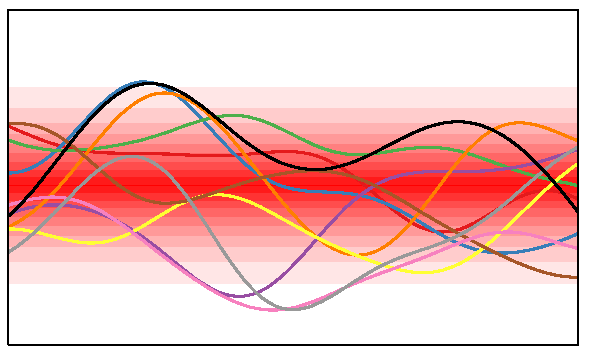
\includegraphics[width=0.48\textwidth]{\introfigsdir/fuzzy-0} & 
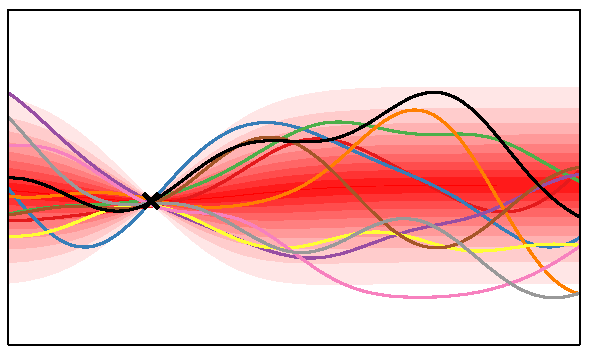
\includegraphics[width=0.48\textwidth]{\introfigsdir/fuzzy-1} \\
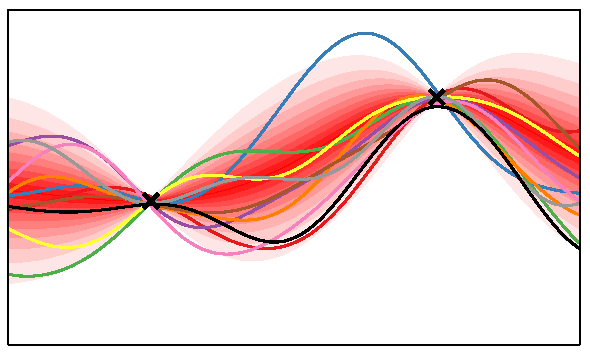
\includegraphics[width=0.48\textwidth]{\introfigsdir/fuzzy-2} & 
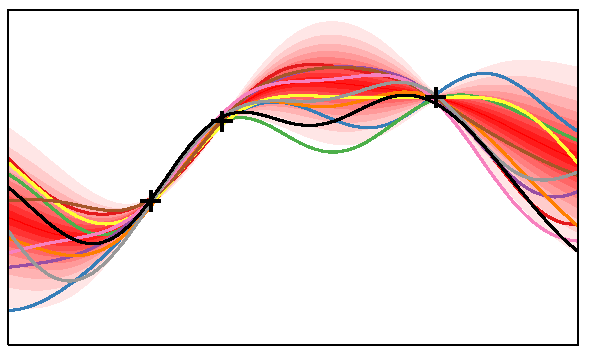
\includegraphics[width=0.48\textwidth]{\introfigsdir/fuzzy-3}
\end{tabular}
\end{centering}
\caption[One-dimensional Gaussian process posterior]{A visual representation of a one-dimensional Gaussian process posterior.
Different shades of red correspond to deciles of the marginal density at each input location.
Coloured lines show samples from the process.
Top left: A \gp{} prior, not conditioned on any datapoints.
Other plots show the posterior as more
}
\label{fig:gp-post}
\end{figure}
%
%Figure \ref{fig:gp-post} shows a Gaussian process distribution, as it is conditioned on more and more observations.
%Typically, it's rendered with the mean and +- 2SD, but there's nothing special about mean.

Gaussian processes are distributions over functions such that any finite subset of function evaluations $f(x_1), f(x_2), \ldots f(x_N)$, have a joint Gaussian distribution \citep{rasmussen38gaussian}.
A \gp{} is completely specified by its mean function,
%
\begin{align}
%\mathbb{E}(f(x)) = \mu(x)
\expectargs{}{f(x)} = \mu(x)
\end{align}
%
and its covariance function, also called the \emph{kernel}:
%
\begin{align}
\Cov(f(x),f(x')) = \kernel(x,x')
\end{align}
%
It is common practice to assume zero mean, since marginalizing over an unknown mean function can be equivalently expressed as a zero-mean \gp{} with a new kernel.

The kinds of structure which can be captured by a \gp{} model is mainly determined by its kernel, which in turn determines how the model generalizes or extrapolates to new data.
One of the main difficulties in using \gp{}s lies in constructing a kernel which can represent the structure present in the data.
%  For small to medium-sized datasets, the kernel has a large impact on modeling efficacy.
%The structure of the kernel captures high-level properties of the unknown function, $f$, 
There are many possible choices of covariance function.
In fact, any symmetric positive-definite function can be used to construct a \gp{} model.
The benefit to this flexibility is that we can specify a wide range of models just by specifying the kernel.
%We can therefore define a language of regression models by specifying a language of kernels.

The class of models that could be called Gaussian processes is extremely broad.
Examples of commonly used models not usually cast as \gp{}s are linear regression, splines, some forms of generalized additive models, and Kalman filters.

Gaussian processes can be seen as a dual representation of Bayesian linear regression. \NA{Cite}
By moving into this dual space, we pay a price in computational complexity, but gain the ability to model functions to any desired level of detail.
Crucially, the marginal likelihood allows us to automatically discover the appropriate amount of detail to use, by Bayesian Occam's razor \citep{rasmussen2001occam,mackay2003information}.

For concreteness, we give the marginal likelihood of the data under a \gp{}:
%
\begin{align}
p(\vy | \vX, \mu(\cdot), k(\cdot, \cdot)) & = \N{\vy}{\mu(\vX)}{k(\vX, \vX)} \nonumber\\
& = (2\pi)^{-\frac{N}{2}}|k(\vX, \vX)|^{-\frac{1}{2}}\, \exp \left\{ -\frac{1}{2} \left( \vy - \boldsymbol\mu(\vX) \right)\tra k(\vX, \vX)\inv \left(\vy - \boldsymbol\mu(\vX) \right) \right\}
\label{eq:gp_marg_lik}
\end{align}
%
The Gaussian likelihood is referred to as the \emph{marginal} likelihood, since it implicitly integrates over all possible functions $\vy$.

Since the marginal likelihood depends on the kernel, we can select the form of the covariance function, or its parameters, by maximum likelihood, or through inference in a Bayesian model.

The predictive distributions also have a simple form:
%
\begin{align}
p( y(\iva^*) | \vy, \vX, \mu(\iva), k(\iva, \iva)) 
= \mathcal{N} \big( y(\iva^*) | & \mu(\iva^*) + k(\iva^*, \vX) k(\vX, \vX)\inv \left( \vy - \mu(\vX) \right)  \nonumber \\
& k(\iva^*, \iva^*) - k(\iva^*, \vX) k(\vX, \vX)\inv k(\vX, \iva^*) \big)
\label{eq:predictive}
\end{align}
%
These equations may look complex, but only require a few matrix operations to evaluate.

Sampling from a \gp{} is also straightforward: a sample from a \gp{} is just a single sample from a single multivariate Normal distribution \eqref{eq:predictive}.
Figure~\ref{fig:gp-post} shows prior and posterior samples from a \gp{}.


%[explain how that works]
% Insert neural net stuff here?

\subsection{Useful properties of Gaussian processes}

\begin{itemize}

\item {\bf Analytic inference}
Given a kernel function and some observations, the predictive posterior distribution can be computed exactly in closed form.  This is a rare property for nonparametric models to have.

\item {\bf Expressivity}
By choosing different covariance functions, we can express a very wide range of modeling assumptions.

\item {\bf Integration over hypotheses}
The fact that a \gp{} posterior lets us exactly integrate over a wide range of hypotheses means that overfitting is less of an issue than in comparable model classes.
It also removes the need for sophisticated optimization schemes.
%
In contrast, much of the neural network literature is devoted to techniques for regularization and optimization.

\item {\bf Marginal likelihood}
A side benefit of being able to integrate over all hyoptheses is that we compute the \emph{marginal likelihood} of the data given the model.
This gives us a principled way of comparing different Gaussian process models.

\item {\bf Closed-form posterior}
The posterior predictive distribution of a \gp{} is another \gp{}.
This means that \gp{}s can easily be composed with other models or decision procedures.
For example, in reinforcement learning applications, 

\item {\bf Easy to Analyze}
%\subsection{Why stick to such a limited model class?}
It may seem unsatisfying to restrict ourselves to a limited model class.
Shouldn't we instead learn to use some more flexible model class, such as the set of all computible functions?
The answer is: simple models can be used as well-understood building blocks for constructing more interesting models in diverse settings.

Consider linear models.
Although they form an extremely limited model class, they are fast, simple, and easy to analyze.
This makes them easy to incorporate into other models or procedures.
Linear models may seem like a hopelessly simple model class, but they're arguably the most useful modeling tools in existence.

\end{itemize}




\subsection{Limitations of Gaussian processes}

\begin{itemize}

\item {\bf Slow inference}
Computing the matrix inverse in \eqref{eq:gp_marg_lik} and \eqref{eq:predictive} takes $\mathcal{O}(N^3)$ time.
%and $\mathcal{O}(N^2)$ memory.  
Fortunately, this problem can be addressed by approximate inference schemes, and most \gp{} software packages implement several of these.

\item {\bf Light tails}
We may wish to use non-Gaussian noise models, for instance in order to be robust to outliers, or to perform classification, or some other form of structured prediction.
Using non-Gaussian noise models requires approximate inference schemes; fortunately, mature software packages exist which can automatically perform approximate inference for a wide variety of likelihoods.
%\item {\bf Symmetric}
%The predictive distribution of a \gp{} is always symmetric about its mean function.
%This means that \gp{} models are inappropriate for modeling non-negative functions, such as likelihoods.
%However, this problem can be addressed by simply exponentiating a \gp{} model, giving rise to a \emph{log-Gaussian process}.

\item {\bf The need to choose a kernel}
In practice, the extreme flexibility of \gp{} models means that we are also faced with the difficult task of choosing a kernel.
In fact, 
%because the model only depends on the inputs through the kernel, 
choosing a useful kernel is equivalent to the problem of learning good features for the data.
Typically, human experts choose from among a small set of standard kernels.
In this thesis, we hope to go some way towards automating the construction and selection of useful kernels.
\end{itemize}





\section{Outline and Contributions of this Thesis}

This thesis presents a set of related results about how the probabilistic nature of Gaussian process models allows them to be easily extended or composed with other models.
Furthermore, the fact that the marginal likelihood is often available (or easily approximable) means that we can evaluate how much evidence the data provides for one structure over another.

\paragraph{Chapter \ref{ch:kernels}} contains a wide-ranging overview of many of the types of structured priors on functions that can be easily expressed by constructing appropriate covariance functions.
%describes, in detail, the ways in which different sorts of structure can be introduced into a \gp{} model through the kernel.
%TODO: Expand this description.
For example, in chapter~\ref{ch:kernels}, we'll see how \gp{}s can be combined with latent variable models to produce models of nonparametric manifolds.
By introducing structure into the kernels of those \gp{}s, we can create manifolds with diverse topological structures, such as cylinders, torii and M\"obius strips.

Given a wide variety of structures, plus the ability to evaluate the suitability of each one, it's straightforward to automatically search over models.
{\bf Chapter \ref{ch:grammar}} shows how to construct a general, open-ended language over kernels - which implies a corresponding language over models.
In chapter~\ref{ch:grammar}, we'll see how the marginal likelihood can guide us into automatically building structured models, and how capturing structure allows us to extrapolate, rather than simply interpolating.

Another benefit of using a relatively simple model class is that the resulting models are easy to understand.
{\bf Chapter~\ref{ch:description}} demonstrates how easy-to-understand the resulting models are, by demonstrating a simple system which automatically describes the structure discovered in a dataset by a search over \gp{} models.
This system automatically generates reports with graphs and english-language descriptions of \gp{} models.
Chapter \ref{ch:description} shows that, for the particular language of models constructed in chapter \ref{ch:grammar}, it's relatively easy to automatically generate english-language descriptions of the models discovered.
Augmented with interpretable plots decomposing the predictive posterior, we demonstrate how to automatically generate useful analyses of time-series.
Combined with the automatic model search developed in chapter \ref{ch:grammar}, this system represents the beginnings of an ``automatic statistician''.
We discuss the advantages and potential pitfalls of automating the modeling process in this way.

{\bf Chapter \ref{ch:additive}} examines the model class obtained by performing dropout in \gp{}s, finding them to have equivalent covariance to \emph{additive Gaussian processes}, a model summing over exponentially-many \gp{} models, each depending on a different subset of the input variables.  An polynomial-time algorithm for doing inference in this model class is given, and the resulting model class is characterized and related to existing model classes.

{\bf Chapter \ref{ch:warped}} develops an extension of the \gplvm{} in which the latent distribution is a mixture of Gaussians.  This model gives rise to a Bayesian clustering model in the clusters have nonparametric shapes.  Like the density manifolds learned by the \gplvm{}, the shapes of the clusters learned by the \iwmm{} follow the contours of the data density.

Besides having a dual representation as linear regression, \gp{}s can also be derived as the limit of an infinitely-wide neural network.
As an example of using \gp{}s as a simple-to-understand building block, {\bf Chapter \ref{ch:deep-limits}} analyzes deep network models by characterizing the prior over functions obtained by composing \gp{} priors to form \emph{deep Gaussian processes}.
%, and relates them to existing neep neural network architecures.
We find that, as the number of layers in such models increases, the amount of information retained about the original input diminshes to a single degree of freedom.
We show that a simple change to the network architecture fixes this pathology.


\section{Attribution}

This thesis was made possible (and enjoyable to produce) by the substantial contributions of the many co-authors I was fortunate to work with.
In this section, I %detail the novel contributions of this thesis, and 
attempt to give proper credit to my tireless co-authors.

\paragraph{Structure through kernels}
%Chapter \ref{ch:kernels} contains a wide-ranging overview of many of the types of structured priors on functions that can be easily expressed by constructing appropriate covariance functions.
Section \ref{sec:deep_kernels} of chapter \ref{ch:kernels}, describing how symmetries in the kernel of a \gplvm{} give rise to priors on manifolds with interesting topologies, is based on a collaboration with David Reshef, Roger Grosse, Josh Tenenbaum, and Zoubin Ghahramani.

\paragraph{Structure Search}
The research upon which Chapter \ref{ch:grammar} is based was done in collaboration with James Robert Lloyd, Roger Grosse, Joshua B. Tenenbaum, and Zoubin Ghahramani, and was published in \citep{DuvLloGroetal13}, where James Lloyd was joint first author.
Myself, James Lloyd and Roger Grosse jointly developed the idea of searching through a grammar-based language of \gp{} models, inspired by \citet{grosse2012exploiting}, and wrote the first versions of the code together.
James Lloyd ran almost all of the experiments.
 Carl Rasmussen, Zoubin Ghahramani and Josh Tenenbaum provided many conceptual insights, as well as suggestions about how the resulting procedure could be most fruitfully applied.

\paragraph{Automatic Statistician} The work appearing in chapter \ref{ch:description} was written in collaboration with James Robert Lloyd, Roger Grosse, Joshua B. Tenenbaum, Zoubin Ghahramani, and was published in \citep{LloDuvGroetal14}.
The idea of the correspondence between kernels and adjectives grew out of discussions between James and myself.
James Lloyd wrote most of the code to automatically generate reports, and ran all of the experiments.
The text was written mainly by myself, James Lloyd, and Zoubin Ghahramani, with many helpful contributions and suggestions from Roger Grosse and Josh Tenenbaum.

\paragraph{Additive Gaussian processes}
The work in chapter \ref{ch:additive} discussing additive \gp{}s was done in collaboration with Hannes Nickisch and Carl Rasmussen, who developed a richly parameterized kernel which efficiently sums all possible products of input dimensions.
My role in the project was to examine the properties of the resulting model, clarify the connections to existing methods, and to create all figures and run all experiments.
This work was previously published in \citep{duvenaud2011additive11}.

\paragraph{Warped Mixtures}
The work comprising the bulk of chapter \ref{ch:warped} was done in collaboration with Tomoharu Iwata and Zoubin Ghahramani, and appeared in \citep{IwaDuvGha12}.
Specifically, the main idea was borne out of a conversation between Tomo and myself, and together we wrote almost all of the code together as well as the paper.
Tomo ran most of the experiments.
Zoubin Ghahramani provided initial guidance, as well as many helpful suggestions throughout the project.


\paragraph{Deep Gaussian Processes}
The ideas contained in chapter \ref{ch:deep-limits} were developed through discussions with Oren Rippel, Ryan Adams and Zoubin Ghahramani, and appear in \citep{DuvRipAdaGha14}.  The derivations, experiments and writing were done mainly by myself, with many helpful suggestions by my co-authors.

\outbpdocument{
\bibliographystyle{plainnat}
\bibliography{references.bib}
}



%
% A header that lets you compile a chapter by itself, or inside a larger document.
% Adapted from http://stackoverflow.com/questions/3655454/conditional-import-in-latex
%
%
%Use \inbpdocument and \outbpdocument in your individual files, in place of \begin{document} and \end{document}. In your main file, put in a \def \ismaindoc {} before including or importing anything.
%
% David Duvenaud
% June 2011
% 
% ======================================
%
%


\ifx\ismaindoc\undefined
	\newcommand{\inbpdocument}{
		\def \ismaindoc {}
		% Use this header if we are compiling by ourselves.
		\documentclass[a4paper,11pt,authoryear,index]{common/PhDThesisPSnPDF}
		
%\usepackage{draftwatermark}
%\SetWatermarkLightness{0.95}

% ******************************************************************************
% ****************************** Custom Margin *********************************

% Add `custommargin' in the document class options to use this section
% Set {innerside margin / outerside margin / topmargin / bottom margin}  and
% other page dimensions

\ifsetMargin
\else
    \RequirePackage[left=37mm,right=30mm,top=35mm,bottom=30mm]{geometry}
    \setFancyHdr % To apply fancy header after geometry package is loaded
\fi


%\chead{Unfinished draft}
%\cfoot{\texttt{Unfinished draft - compiled on \today{} at \currenttime}}

% *****************************************************************************
% ******************* Fonts (like different typewriter fonts etc.)*************

% Add `customfont' in the document class option to use this section

\ifsetFont
\else
    % Set your custom font here and use `customfont' in options. Leave empty to
    % load computer modern font (default LaTeX font).  

    \RequirePackage{libertine} 
\fi

% *****************************************************************************
% *************************** Bibliography  and References ********************

%\usepackage{cleveref} %Referencing without need to explicitly state fig /table

% Add `custombib' in the document class option to use this section
\ifsetBib % True, Bibliography option is chosen in class options
\else % If custom bibliography style chosen then load bibstyle here

   \RequirePackage[square, sort, numbers, authoryear]{natbib} % CustomBib

% If you would like to use biblatex for your reference management, as opposed to the default `natbibpackage` pass the option `custombib` in the document class. Comment out the previous line to make sure you don't load the natbib package. Uncomment the following lines and specify the location of references.bib file

% \RequirePackage[backend=biber, style=numeric-comp, citestyle=numeric, sorting=nty, natbib=true]{biblatex}
% \bibliography{References/references} %Location of references.bib only for biblatex

\fi


% changes the default name `Bibliography` -> `References'
\renewcommand{\bibname}{References}


% *****************************************************************************
% *************** Changing the Visual Style of Chapter Headings ***************
% Uncomment the section below. Requires titlesec package.

%\RequirePackage{titlesec}
%\newcommand{\PreContentTitleFormat}{\titleformat{\chapter}[display]{\scshape\Large}
%{\Large\filleft{\chaptertitlename} \Huge\thechapter}
%{1ex}{}
%[\vspace{1ex}\titlerule]}
%\newcommand{\ContentTitleFormat}{\titleformat{\chapter}[display]{\scshape\huge}
%{\Large\filleft{\chaptertitlename} \Huge\thechapter}{1ex}
%{\titlerule\vspace{1ex}\filright}
%[\vspace{1ex}\titlerule]}
%\newcommand{\PostContentTitleFormat}{\PreContentTitleFormat}
%\PreContentTitleFormat


% *****************************************************************************
% **************************** Custom Packages ********************************
% *****************************************************************************


% ************************* Algorithms and Pseudocode **************************

%\usepackage{algpseudocode} 


% ********************Captions and Hyperreferencing / URL **********************

% Captions: This makes captions of figures use a boldfaced small font. 
%\RequirePackage[small,bf]{caption}

\RequirePackage[labelsep=space,tableposition=top]{caption} 
%\renewcommand{\figurename}{Figure} %to support older versions of captions.sty
\captionsetup{belowskip=12pt,aboveskip=4pt}

% ************************ Formatting / Footnote *******************************

%\usepackage[perpage]{footmisc} %Range of footnote options 


% ****************************** Line Numbers **********************************

%\RequirePackage{lineno}
%\linenumbers

% ************************** Graphics and figures *****************************

%\usepackage{rotating}
%\usepackage{wrapfig}
%\usepackage{float}
\usepackage{subfig} %note: subfig must be included after the `caption` package. 


% ********************************* Table **************************************

%\usepackage{longtable}
%\usepackage{multicol}
%\usepackage{multirow}
%\usepackage{tabularx}


% ***************************** Math and SI Units ******************************

\usepackage{amsfonts}
\usepackage{amsmath}
\usepackage{amssymb}
%\usepackage{siunitx} % use this package module for SI units


% ******************************************************************************
% ************************* User Defined Commands ******************************
% ******************************************************************************

% *********** To change the name of Table of Contents / LOF and LOT ************

%\renewcommand{\contentsname}{My Table of Contents}
%\renewcommand{\listfigurename}{List of figures}
%\renewcommand{\listtablename}{List of tables}


% ********************** TOC depth and numbering depth *************************

\setcounter{secnumdepth}{2}
\setcounter{tocdepth}{2}

% ******************************* Nomenclature *********************************

% To change the name of the Nomenclature section, uncomment the following line

%\renewcommand{\nomname}{Symbols}


% ********************************* Appendix ***********************************

% The default value of both \appendixtocname and \appendixpagename is `Appendices'. These names can all be changed via: 

%\renewcommand{\appendixtocname}{List of appendices}
%\renewcommand{\appendixname}{Appndx}

		% All my custom preamble stuff.  Shouldn't overlap with anything in official-preamble


% Paths to figure and table directories.
\newcommand{\symmetryfigsdir}{figures/symmetries}
\newcommand{\topologyfiguresdir}{figures/topology}
\newcommand{\infinitefiguresdir}{figures/infinite}
\newcommand{\grammarfiguresdir}{figures/grammar}
\newcommand{\introfigsdir}{figures/intro}
\newcommand{\gplvmfiguresdir}{figures/gplvm}
\newcommand{\warpedfiguresdir}{figures/warped-mixtures}
\newcommand{\deeplimitsfiguresdir}{figures/deep-limits}
\newcommand{\quadraturefigsdir}{figures/quadrature}
\newcommand{\additivefigsdir}{figures/additive}
\newcommand{\decompfigsdir}{figures/decomp}
\newcommand{\examplefigsdir}{figures/worked-example}


\usepackage{bm}  % for warped mixtures - is this necessary?
\usepackage{booktabs}
\usepackage{tabularx}
\usepackage{multirow}
\usepackage{datetime}
\renewcommand{\tabularxcolumn}[1]{>{\arraybackslash}m{#1}}
\usepackage{relsize}
\usepackage{graphicx}
\usepackage{amsmath,amssymb,textcomp}
\usepackage{nicefrac}
\usepackage{amsthm}
\usepackage{tikz}
\usetikzlibrary{arrows}
\usetikzlibrary{calc}
\usepackage{nth}
\usepackage{rotating}
\usepackage{array}
\usepackage{fp}
\usepackage[hyperpageref]{backref}
\def\foo{\hspace{\fill}\mbox{}\linebreak[0]\hspace*{\fill}}
\renewcommand*{\backref}[1]{}
\renewcommand*{\backrefalt}[4]{%
\ifcase #1 %
%
\or
\foo(page #2)%
\else
\foo(pages #2)%
\fi
}

\usepackage{cleveref}
\crefname{equation}{equation}{equations}


%% For submission, make all render blank.
\input{common/commenting.tex}
%\renewcommand{\LATER}[1]{}
%\renewcommand{\fLATER}[1]{}
%\renewcommand{\TBD}[1]{}
%\renewcommand{\fTBD}[1]{}
%\renewcommand{\PROBLEM}[1]{}
%\renewcommand{\fPROBLEM}[1]{}
%\renewcommand{\NA}[1]{}


% HUMBLE WORDS: shown slightly smaller when in normal text
% Thanks to Christian Steinruecken!
\input{common/humble.tex}


% TODO: Clean up duplicates
\declareHumble{ANOVA}{ANOVA}
\declareHumble{ARD}{ARD}
\declareHumble{BIC}{BIC}
\declareHumble{BMC}{BMC}
\declareHumble{bq}{BQ}
\declareHumble{CRP}{CRP}
\declareHumble{dirpro}{DP}
\declareHumble{HDMR}{HDMR}
\declareHumble{GAM}{GAM}
\declareHumble{GEM}{GEM}
\declareHumble{GMM}{GMM}
\declareHumble{gplvm}{GP-LVM}
\declareHumble{gpml}{GPML}
\declareHumble{GPML}{GPML}
\declareHumble{gprn}{GPRN}
\declareHumble{gpt}{GP}
\declareHumble{gp}{GP}
\declareHumble{HKL}{HKL}
\declareHumble{HMC}{HMC}
\declareHumble{ibp}{IBP}
\declareHumble{iGMM}{iGMM}
\declareHumble{iwmm}{iWMM}
\declareHumble{kCP}{CP}
\declareHumble{kCW}{CW}
\declareHumble{kC}{C}
\declareHumble{KDE}{KDE}
\declareHumble{kLin}{Lin}
\declareHumble{KPCA}{KPCA}
\declareHumble{kPer}{Per}
\declareHumble{kRQ}{RQ}
\declareHumble{kSE}{SE}
\declareHumble{kWN}{WN}
\declareHumble{Lin}{Lin}
\declareHumble{LBFGS}{L-BFGS}
\declareHumble{mcmc}{MCMC}
\declareHumble{MKL}{MKL}
\declareHumble{MLP}{MLP}
\declareHumble{MSE}{MSE}
\declareHumble{Per}{Per}
\declareHumble{RMSE}{RMSE}
\declareHumble{RQ}{RQ}
\declareHumble{SBQ}{SBQ}
\declareHumble{seard}{SE-ARD}
\declareHumble{sefull}{SE-\textnormal{full}}
\declareHumble{SEGP}{SE-GP}
\declareHumble{SE}{SE}
\declareHumble{SNR}{SNR}
\declareHumble{SSANOVA}{SS-ANOVA}
\declareHumble{SVM}{SVM}

\newcommand{\kSig}{\boldsymbol\sigma}

\def\subexpr{{\cal S}}
\def\baseker{{\cal B}}
\def\numWinners{k}

\def\ie{i.e.\ }
\def\eg{e.g.\ }
\def\etc{etc.\ }
\let\oldemptyset\emptyset
\let\emptyset 0




% Unify notation between neural-net land and GP-land.
\newcommand{\hphi}{h}
\newcommand{\hPhi}{\vh}
\newcommand{\walpha}{w}
\newcommand{\wboldalpha}{\bw}
\newcommand{\wcapalpha}{\vW}
\newcommand{\lengthscale}{w}

\newcommand{\layerindex}{\ell}



\newcommand{\gpdrawbox}[1]{
\setlength\fboxsep{0pt}
\hspace{-0.15in} 
\fbox{
\includegraphics[width=0.464\columnwidth]{\deeplimitsfiguresdir/deep_draws/deep_gp_sample_layer_#1}
}}



\newcommand{\procedurename}{ABCD}
\newcommand{\genText}[1]{{\sf #1}}



\newcommand{\asdf}{$^{\textnormal{th}}$}

\newcommand{\binarysum}{\sum_{\bf{x} \in \{0,1\}^D}}
\newcommand{\expect}{\mathbb{E}}
\newcommand{\expectargs}[2]{\mathbb{E}_{#1} \left[ {#2} \right]}
\newcommand{\var}{\mathbb{V}}
\newcommand{\varianceargs}[2]{\mathbb{V}_{#1} \left[ {#2} \right]}
\newcommand{\cov}{\operatorname{cov}}
\newcommand{\Cov}{\operatorname{Cov}}
\newcommand{\covargs}[2]{\cov \left[ {#1}, {#2} \right]}
\newcommand{\variance}{\mathbb{V}}
\newcommand{\vecop}[1]{\operatorname{vec} \left( {#1} \right)}

\newcommand{\covarianceargs}[2]{\Cov_{#1} \left[ {#2} \right]}
\newcommand{\colvec}[2]{\left[ \begin{array}{c} {#1} \\ {#2} \end{array} \right]}
\newcommand{\tbtmat}[4]{\left[ \begin{array}{cc} {#1} & {#2} \\ {#3} & {#4} \end{array} \right]}

%\newcommand{\covskinny}[2]{\var\!\left(#1\middle\vert#2\right)} 

\newcommand{\acro}[1]{{\humble{#1}}}
%\newcommand{\vect}[1]{\boldsymbol{#1}}
\newcommand{\vect}[1]{{\bf{#1}}}
\newcommand{\mat}[1]{\mathbf{#1}}
\newcommand{\pderiv}[2]{\frac{\partial #1}{\partial #2}}
\newcommand{\npderiv}[2]{\nicefrac{\partial #1}{\partial #2}}

\newcommand{\pha}{^{\phantom{:}}}

\newcommand{\argmin}{\operatornamewithlimits{argmin}}
\newcommand{\argmax}{\operatornamewithlimits{argmax}}

% The following designed for probabilities with long arguments

\newcommand{\Prob}[2]{P\!\left(\,#1\;\middle\vert\;#2\,\right)}
\newcommand{\ProbF}[3]{P\!\left(\,#1\!=\!#2\;\middle\vert\;#3\,\right)}
\newcommand{\p}[2]{p\!\left(#1\middle\vert#2\right)}
\newcommand{\po}[1]{p\!\left(#1\right)}
\newcommand{\pF}[3]{p\!\left(\,#1\!=\!#2\;\middle\vert\;#3\,\right)} 
\newcommand{\mean}[2]{{m}\!\left(#1\middle\vert#2\right)}



\newcommand{\valpha}{\boldsymbol{\alpha}}
\newcommand{\va}{\vect{a}}
\newcommand{\vA}{\vect{A}}
\newcommand{\vB}{\mat{B}}
\newcommand{\vb}{\vect{b}}
\newcommand{\vC}{\mat{C}}
\newcommand{\vc}{\vect{c}}
\newcommand{\vecf}{\boldsymbol{f}}
\newcommand{\vell}{\vect{\ell}}
\newcommand{\vepsilon}{\boldsymbol{\epsilon}}
\newcommand{\veps}{\boldsymbol{\epsilon}}
\newcommand{\ve}{\boldsymbol{\epsilon}}
\newcommand{\vf}{\vecf}
\newcommand{\vg}{\vect{g}}
\newcommand{\vh}{\vect{h}}
\newcommand{\vI}{\mat{I}}
\newcommand{\vK}{\mat{K}}
\newcommand{\vk}{\vect{k}}
\newcommand{\vL}{\mat{L}}
\newcommand{\vl}{\vect{l}}
\newcommand{\vmu}{\boldsymbol{\mu}}
\newcommand{\vone}{\vect{1}}
\newcommand{\vphi}{\boldsymbol{\phi}}
\newcommand{\vpi}{\boldsymbol{\pi}}
\newcommand{\vq}{\vect{q}}
\newcommand{\vR}{\mat{R}}
\newcommand{\vr}{\vect{r}}
\newcommand{\vsigma}{\boldsymbol{\sigma}}
\newcommand{\vSigma}{\mat{\Sigma}}
\newcommand{\vS}{\mat{S}}
\newcommand{\vs}{\vect{s}}
\newcommand{\vtheta}{\boldsymbol{\theta}}
\newcommand{\vu}{\vect{u}}
\newcommand{\vV}{\mat{V}}
\newcommand{\vW}{\mat{W}}
\newcommand{\vw}{\vect{w}}
\newcommand{\vX}{\mat{X}}
\newcommand{\vx}{\vect{x}}
\newcommand{\vY}{\mat{Y}}
\newcommand{\vy}{\vect{y}}
\newcommand{\vzero}{\vect{0}}
\newcommand{\vZ}{\mat{Z}}
\newcommand{\vz}{\vect{z}}


\newcommand{\netweights}{\alpha}
\newcommand{\vnetweights}{\valpha}

\newcommand{\He}{\mathcal{H}}
\newcommand{\normx}[2]{\left\|#1\right\|_{#2}}
\newcommand{\Hnorm}[1]{\normx{#1}{\He}}
\newcommand{\mmd}{{\rm MMD}}


\newcommand{\mf}{\bar{\vf}}

%\newcommand{\mf}{\mu} %{\bar{\ell}}
\newcommand{\lf}{f} % Likelihood function
\newcommand{\st}{_\star}

% from simpler log-bq writeup
\newcommand{\lftwo}{{\log \ell}}
\newcommand{\mftwo}{{\bar \ell}}
\newcommand{\loggp}{{\log\acro{GP}}}%| \bX, \vy )}}
\newcommand{\loggpdist}{{\acro{GP}(\lftwo)}}%| \vX, \vy )}}


\newcommand{\inv}{^{{\mathsmaller{-1}}}}
\newcommand{\tohalf}{^{{\mathsmaller{\nicefrac{1}{2}}}}}

\newcommand{\Normal}{\mathcal{N}}
\newcommand{\N}[3]{\mathcal{N}\!\left(#1 \middle| #2,#3\right)}
\newcommand{\Nt}[2]{\mathcal{N}\!\left(#1,#2\right)}
\newcommand{\NT}[2]{\mathcal{N}\!\left(#1,#2\right)}
\newcommand{\GPdist}[3]{\mathcal{GP}\!\left(#1 \, \middle| \, #2, #3 \right)}
\newcommand{\bN}[3]{\mathcal{N}\big(#1 \middle| #2,#3\big)}
\newcommand{\boldN}[3]{\text{\textbf{\mathcal{N}}}\big(#1;#2,#3\big)}
\newcommand{\ones}[1]{\mat{1}_{#1}}
\newcommand{\eye}[1]{\mat{E}_{#1}}
\newcommand{\tra}{^{\mathsf{T}}}
%\newcommand{\tra}{^{\top}}
%\mathsf{T}
\newcommand{\trace}{\operatorname{tr}}
\newcommand{\shift}{\operatorname{shift}}
\renewcommand{\mod}{\operatorname{mod}}
\newcommand{\deq}{:=}
\newcommand{\oneofk}{\operatorname{one-of-k}}
%\newcommand{\degree}{^\circ}

\newcommand{\GPt}[2]{\mathcal{GP}\!\left(#1,#2\right)}
%\newcommand{\GPt}[2]{\gp\!\left(#1,#2\right)}

\DeclareMathOperator{\tr}{tr}
\DeclareMathOperator{\chol}{chol}
\DeclareMathOperator{\diag}{diag}

\newenvironment{narrow}[2]{%
  \begin{list}{}{%
  \setlength{\topsep}{0pt}%
  \setlength{\leftmargin}{#1}%
  \setlength{\rightmargin}{#2}%
  \setlength{\listparindent}{\parindent}%
  \setlength{\itemindent}{\parindent}%
  \setlength{\parsep}{\parskip}}%
\item[]}{\end{list}}



\newcommand{\dist}{\ \sim\ }
\def\given{\,|\,}

% Table stuff
\newcolumntype{C}[1]{>{\centering\let\newline\\\arraybackslash\hspace{0pt}}m{#1}}
\newcolumntype{L}[1]{>{\raggedright\let\newline\\\arraybackslash\hspace{0pt}}m{#1}}
\newcolumntype{R}[1]{>{\raggedleft\let\newline\\\arraybackslash\hspace{0pt}}m{#1}}


\def\ie{i.e.\ }
\def\eg{e.g.\ }
\def\iid{i.i.d.\ }
%\def\simiid{\sim_{\mbox{\tiny iid}}}
\def\simiid{\overset{\mbox{\tiny iid}}{\sim}}
\def\simind{\overset{\mbox{\tiny \textnormal{ind}}}{\sim}}
\def\eqdist{\stackrel{\mbox{\tiny d}}{=}}
%\newcommand{\distas}[1]{\mathbin{\overset{#1}{\kern \z@ \sim}}}
%TODO: fix this - it worked outside the thesis!
\newcommand{\distas}[1]{\mathbin{\overset{#1}{\sim}}}

\def\Reals{\mathbb{R}}

\def\Uniform{\mbox{\rm Uniform}}
\def\Bernoulli{\mbox{\rm Bernoulli}}
\def\GP{\mathcal{GP}}
\def\GPLVM{\mathcal{GP-LVM}}




% Kernel stuff

\def\iva{\vect{\inputVar}}
\def\ivaone{\inputVar}
\def\inputVar{x}
\def\InputVar{X}
\def\InputSpace{\mathcal{X}}
\def\outputVar{y}
\def\OutputSpace{\mathcal{Y}}
\def\function{f}
\def\kernel{k}
\def\KernelMatrix{K}
\def\SumKernel{\sum}
\def\ProductKernel{\prod}
\def\expression{e}
\def\feat{\vh}

\newcommand{\kerntimes}{ \! \times \!}
\newcommand{\kernplus}{ \, + \,}


% Proof stuff
\theoremstyle{plain}
\newtheorem{theorem}{Theorem}[section]
\newtheorem{lemma}[theorem]{Lemma}
\newtheorem{prop}[theorem]{Proposition}
\newtheorem{proposition}{Proposition}
\newtheorem*{cor}{Corollary}

% For infinite bq
\newcommand{\iv}{\theta}
\newcommand{\viv}{\vtheta}

% For intro chapter
\newcommand{\funcval}{\vf(\vX)}
\newcommand{\testpoint}{{\vx^\star}}

\newcommand{\underwrite}[2]{{\underbrace{#1}_{\textnormal{#2}}}}



% For kernel figures
\newcommand{\fhbig}{2cm}%
\newcommand{\fwbig}{3cm}%
\newcommand{\kernpic}[1]{\includegraphics[height=\fhbig,width=\fwbig]{\grammarfiguresdir/structure_examples/#1}}%
\newcommand{\kernpicr}[1]{\rotatebox{90}{\includegraphics[height=\fwbig,width=\fhbig]{\grammarfiguresdir/structure_examples/#1}}}%
\newcommand{\addkernpic}[1]{{\includegraphics[height=\fhbig,width=\fwbig]{\grammarfiguresdir/additive_multi_d/#1}}}%
\newcommand{\largeplus}{\tabbox{{\Large+}}}%
\newcommand{\largeeq}{\tabbox{{\Large=}}}%
\newcommand{\largetimes}{\tabbox{{\Large$\times$}}}%
\newcommand{\fixedx}{$x$ (with $x' = 1$)}%


		% ************************ Thesis Information & Meta-data **********************

%% The title of the thesis
%\title{Structured Gaussian Process Models} 
%\title{Automatic Model Construction \\ through \\ Structured Gaussian Processes}
%\title{Automatic Model-Building \\ through \\ Structured Gaussian Processes}
%\title{Automatic Modeling \\ with \\ Structured Gaussian Processes}    
\title{Automatic Model Construction \\ with Gaussian Processes}
%\title{Automatic Model Construction}
%\title{Automating Statistical Model Construction}


%\texorpdfstring is used for PDF metadata. Usage:
%\texorpdfstring{LaTeX_Version}{PDF Version (non-latex)} eg.,
%\texorpdfstring{$sigma$}{sigma}

%% The full name of the author
\author{David Kristjanson Duvenaud}

%% Department (eg. Department of Engineering, Maths, Physics)
%\dept{Department of Engineering}

%% University and Crest
\university{University of Cambridge}
\crest{
\includegraphics[width=0.25\textwidth]{University_Crest}}

%% You can redefine the submission text:
% Default as per the University guidelines: This dissertation is submitted for
% the degree of Doctor of Philosophy
%\renewcommand{\submissiontext}{change the default text here if needed}

%% Full title of the Degree 
\degree{Doctor of Philosophy}
 
%% College affiliation (optional)
\college{Pembroke College}

%% Submission date
\degreedate{June 2014} 

%% Meta information
\subject{LaTeX} \keywords{{LaTeX} {PhD Thesis} {Engineering} {University of Cambridge}}



		\begin{document}
	}	
	\newcommand{\outbpdocument}[1]{

		% Fake chapters so references aren't broken
\label{ch:intro}                
\label{ch:kernels}
\label{ch:grammar}
\label{ch:description}
\label{ch:additive}
\label{ch:deeplimits}
\label{ch:discussion}
		%\bibliographystyle{common/CUEDthesis}
		\bibliographystyle{plainnat}
		\bibliography{references.bib}
		\end{document}
	}	
\else
	%If we're inside another document, no need to re-start the document.
	\ifx\inbpdocument\undefined
		\newcommand{\inbpdocument}{}
		\newcommand{\outbpdocument}[1]{}
	\fi
\fi

\inbpdocument

\chapter{Expressing Structure with Kernels}
\label{ch:kernels}

This chapter shows how to use kernels to build models of functions with many different kinds of structure: additivity, symmetry, periodicity, interactions between variables, and changepoints.
We will also show several ways to encode group invariants into kernels.
Combining a few simple kernels through addition and multiplication will give us a rich, open-ended language of models.

The properties of kernels discussed in this chapter are mostly known in the literature.
The original contribution of this chapter is to gather them into a coherent whole and to offer a tutorial showing the implications of different kernel choices, and some of the structures which can be obtained by combining them.
To the best of our knowledge, the different types of structure that could be obtained through sums and products of kernels had not been systematically explored before \citet{DuvLloGroetal13}.
%TODO: Add more about contribution here.


\section{Definition}

%Since we'll be discussing kernels at length, we now give a precise definition.
A kernel (also called a covariance function, kernel function, or covariance kernel), is a positive-definite function of two inputs $\vx, \vx'$. % in some space $\InputSpace$. 
%Formally, we write $\kernel(\vx, \vx'): \InputSpace \times \InputSpace \to \Reals$.
In this chapter, $\vx$ and $\vx'$ are usually vectors in a Euclidean space, but kernels can also be defined on graphs, images, discrete or categorical inputs, or even text.

Gaussian process models use a kernel to define the prior covariance between any two function values:
%
\begin{align}
\textrm{Cov}\left(f(\vx), f(\vx') \right) = \kernel(\vx,\vx')
\end{align}
%
Colloquially, kernels are often said to specify the similarity between two objects.
This is slightly misleading in this context, since what is actually being specified is the similarity between two values of a \emph{function} evaluated on each object.
The kernel specifies which functions are likely under the \gp{} prior, which in turn determines the generalization properties of the model.





\section{A few basic kernels}
\label{sec:basic-kernels}

To begin understanding the types of structures expressible by \gp{}s, we will start by briefly examining the priors on functions encoded by some commonly used kernels:
the squared-exponential (\kSE), periodic (\kPer), and linear (\kLin) kernels.
These kernels are defined in \cref{fig:basic_kernels}.
%
\begin{figure}[h]%
\centering
\begin{tabular}{r|ccc}
Kernel name: & Squared-exp (\kSE) & Periodic (\kPer) & Linear (\kLin) \\[10pt]
$k(x, x') =$ & $\sigma_f^2 \exp\left(-\frac{(\inputVar - \inputVar')^2}{2\ell^2}\right)$ &
$\sigma_f^2 \exp\left(-\frac{2}{\ell^2} \sin^2 \left( \pi \frac{\inputVar - \inputVar'}{p} \right)\right)$ &
$\sigma_f^2 (\inputVar - c)(\inputVar' - c)$ \\[14pt]
\raisebox{1cm}{Plot of kernel:} & \kernpic{se_kernel} & \kernpic{per_kernel} & \kernpic{lin_kernel}\\
& $x -x'$ & $x -x'$ & \fixedx \\
%& & & \\
 & \large $\downarrow$ & \large $\downarrow$ & \large $\downarrow$  \\
\raisebox{1cm}{\parbox{2.5cm}{Samples from \gp{} prior:}} & \kernpic{se_kernel_draws} & \kernpic{per_kernel_draws_s2} & \kernpic{lin_kernel_draws} \\
Type of structure: & local variation & repeating structure & linear functions
\end{tabular}
\vspace{6pt}
\caption[Examples of structures expressible by some basic kernels]
{Examples of structures expressible by some basic kernels.
%Left and third columns: base kernels $k(\cdot,0)$.
%Second and fourth columns: draws from a \sgp{} with each repective kernel.
%The x-axis has the same range on all plots.
}
\label{fig:basic_kernels}
\end{figure}
%
%There is nothing special about these kernels in particular, except that they represent a diverse set.

Each covariance function corresponds to a different set of assumptions made about the function we wish to model.
For example, using a squared-exp ($\kSE$) kernel implies that the function we are modeling has infinitely many derivatives.
There exist many variants of ``local'' kernels similar to the $\kSE$ kernel, each encoding slightly different assumptions about the smoothness of the function being modeled.

\paragraph{Kernel parameters}
Each kernel has a number of parameters which specify the precise shape of the covariance function.
These are sometimes referred to as \emph{hyper-parameters}, since they can be viewed as specifying a distribution over function parameters, instead of being parameters which specify a function directly.


\paragraph{Stationary and Non-stationary}
The $\kSE$ and $\kPer$ kernels are \emph{stationary}, meaning that their value only depends on the difference $x-x'$.  This implies that the probability of observing a particular dataset remains the same even if we move all the $\vx$ values over by some amount.
In contrast, the linear kernel $\kLin$ is non-stationary, meaning that the corresponding \gp{} model will produce different answers if the data is moved around while the kernel parameters are kept fixed.




\section{Combining kernels}

What if the kind of structure we need is not expressed by any existing kernel?
For many types of structure, it is possible to build a ``made to order'' kernel with the desired properties.
The next few sections of this chapter will explore ways in which kernels can be combined to create new ones with different properties.
This will allow us to include as much high-level structure as necessary into our models.
%For an overview, see \cite[Chapter~4]{rasmussen38gaussian}.


\subsection{Notation}

Below, we will focus on two ways of combining kernels: addition and multiplication.
We will often write these operations in shorthand, without arguments:
%
\begin{align}
k_a + k_b =& \,\, k_a(\vx, \vx') + k_b( \vx, \vx')\\
k_a \times k_b =& \,\, k_a(\vx, \vx') \times k_b(\vx, \vx')
\end{align}

All of the basic kernels we considered in \cref{sec:basic-kernels} are one-dimensional, but kernels over multidimensional inputs can be constructed by adding and multiplying between kernels on different dimensions.
The dimension on which a kernel operates is denoted by a subscripted integer.
For example, $\SE_2$ represents an \kSE{} kernel over the second dimension of $\vx$.
To remove clutter, we will usually refer to kernels without specifying their parameters.



\subsection{Combining properties through multiplication}

%Multiplying kernels allows us to account for interactions between different input dimensions, or to combine different notions of similarity.

%Loosely speaking, multip

Multiplying two positive-definite kernels together always results in another positive-definite kernel.
But what properties do these new kernels have?
%
\begin{figure}
\centering
\begin{tabular}{cccc}
$\kLin \times \kLin$ & $\kSE \times \kPer$ & $\kLin \times \kSE$ & $\kLin \times \kPer$ \\
\kernpic{lin_times_lin} & \kernpic{longse_times_per} & \kernpic{se_times_lin} & \kernpic{lin_times_per}\\
\fixedx & $x -x'$ & \fixedx & \fixedx\\
%& & & \\
\large $\downarrow$ & \large $\downarrow$ & \large $\downarrow$ & \large $\downarrow$  \\
\kernpic{lin_times_lin_draws}  & \kernpic{longse_times_per_draws_s2} & \kernpic{se_times_lin_draws_s2} & \kernpic{lin_times_per_draws_s2} \\
quadratic functions & locally \newline periodic & increasing variation  & growing amplitude \\[10pt]
\end{tabular}
\caption[Examples of structures expressible by multiplying kernels]
{ Examples of one-dimensional structures expressible by multiplying kernels.  
%The x-axis has the same scale for all plots.
Plots have same meaning as in figure \ref{fig:basic_kernels}.}
\label{fig:kernels_times}
\end{figure}
%
\Cref{fig:kernels_times} shows some more interesting kernels that one can obtain by multiplying two basic kernels together.

Working with kernels rather than the parametric form of the function itself allows us to express high-level properties of functions that do not necessarily have a simple parametric form.
Here, we discuss a few examples:

\begin{itemize}
\item {\bf Polynomial Regression.}
By multiplying together $T$ linear kernels, we obtain a prior on polynomials of degree $T$.
The first column of \cref{fig:kernels_times} shows a quadratic kernel.

\item {\bf Locally Periodic Functions.}
In univariate data, multiplying a kernel by \kSE{} gives a way of converting global structure to local structure.
For example, $\Per$ corresponds to exactly periodic structure, whereas $\Per \kerntimes \SE$ corresponds to locally periodic structure, as shown in the second column of \cref{fig:kernels_times}.

\item {\bf Functions with Growing Amplitude.}
Multiplying by a linear kernel means that the marginal standard deviation of the function being modeled will grow linearly away from the origin.
The third and fourth columns of \cref{fig:kernels_times} show two examples.
\end{itemize}

We can multiply any number of kernels together in this way to produce kernels combining several high-level properties.
For example, the kernel $\kSE \kerntimes \kLin \kerntimes \kPer$ is a prior on functions which are locally periodic with linearly growing amplitude.
We will see examples of real datasets with this kind of structure in \cref{ch:grammar}.


\subsection{Building flexible multidimensional models}

%For instance, in multidimensional data, the multiplicative kernel $\SE_1 \kerntimes \SE_2$ represents a smoothly varying function of dimensions 1 and 2 which is not constrained to be additive.

We can build flexible models of functions of more than one input simply by multiplying kernels between the different inputs.
For example, a product of $\kSE$ kernels over different dimensions, each having a different lengthscale parameter, is called the $\seard$ kernel:
%
\begin{align}
\seard( \vx, \vx')
 = \prod_{d=1}^D \exp \sigma_d^2 \left( -\frac{1}{2} \frac{\left( x_d - x'_d \right)^2}{\ell_d^2} \right)
 = \sigma_f^2 \exp \left( -\frac{1}{2} \sum_{d=1}^D \frac{\left( x_d - x'_d \right)^2}{\ell_d^2} \right)
\end{align}
%
\Cref{fig:product-of-se-kernels} illustrates the \seard{} kernel in two dimensions.
%
\begin{figure}[ht!]
\centering
\begin{tabular}{ccccccc}
%$\kSE_1$ & \hspace{-0.4cm} $\kerntimes$ & $\kSE_2$ &  $=$ & \hspace{-0.4cm} $\kSE_1 \kerntimes \kSE_2$ & & \hspace{-0.5cm} $f \sim \GPt{\vzero}{\kSE_1 \kerntimes \kSE_2}$ \\
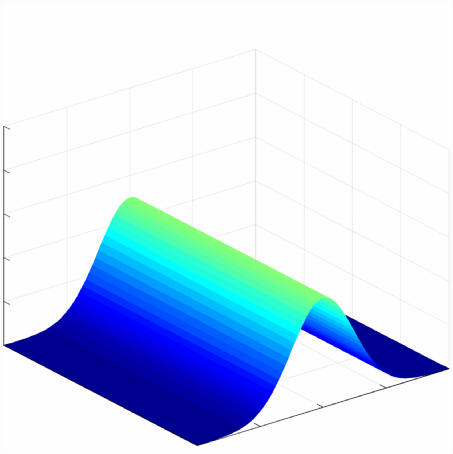
\includegraphics[width=0.2\textwidth]{\additivefigsdir/2d-kernel/additive_kernel_sum_p1} \hspace{-0.3cm}
& \hspace{-0.3cm} \raisebox{1cm}{$\times$} & 
\hspace{-0.3cm}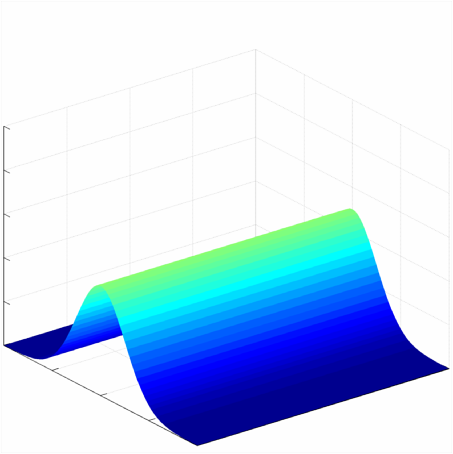
\includegraphics[width=0.2\textwidth]{\additivefigsdir/2d-kernel/additive_kernel_sum_p2} \hspace{-0.3cm}
& \hspace{-0.2cm} \raisebox{1cm}{=} \hspace{-0.2cm} & \hspace{-0.3cm}
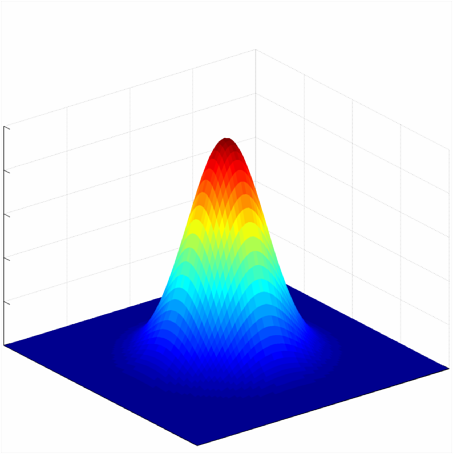
\includegraphics[width=0.2\textwidth]{\additivefigsdir/2d-kernel/sqexp_kernel} 
& \hspace{-0.3cm} \raisebox{1cm}{$\rightarrow$} \hspace{-0.3cm} & \hspace{-0.3cm}
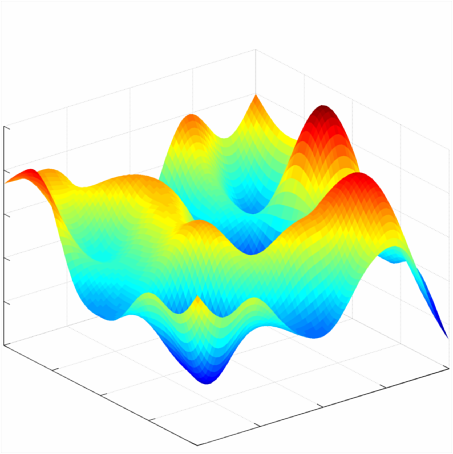
\includegraphics[width=0.2\textwidth]{\additivefigsdir/2d-kernel/sqexp_draw}\\
%$k_1(x_1, x_1')$ & & $k_2(x_2, x_2')$ & & \hspace{-0.4cm}\parbox{4cm}{$k_1(x_1,x_1') \kerntimes k_2(x_2,x_2')$} & & $f(x_1, x_2)$ \\[1em]
$\kSE_1(x_1, x_1')$ &  & $\kSE_2(x_2, x_2')$ &  & \hspace{-0.4cm} $\kSE_1 \kerntimes \kSE_2$ & & \hspace{-0.5cm} \parbox{0.24\columnwidth}{$f(x_1, x_2)$ drawn from $\GPt{0}{\kSE_1 \kerntimes \kSE_2}$} \\
\end{tabular}
\caption[A product of squared-exponential kernels across different dimensions]{
%\emph{Top left:} An additive kernel is a sum of kernels.
%\emph{Bottom left:}  A draw from an additive kernel corresponds to a sum of draws from independent \gp{} priors with the corresponding kernels.
%\emph{Top right:} A product kernel.
%\emph{Right:}  A \gp{} prior with a product of kernels does not correspond to a product of draws from \gp{}s.
%In this example, both kernels are composed of one dimensional squared-exponential kernels, but this need not be the case in general.
A product of two one-dimensional kernels gives rise to a prior on functions which depend on both dimensions.
}
\label{fig:product-of-se-kernels}
\end{figure}

\ARD{} stands for Automatic Relevance Determination, so named because estimating the lengthscale parameters $\ell_1, \ell_2, \dots, \ell_D$, implicitly determines the ``relevance'' of each dimension.
Input dimensions with relatively large lengthscales indicate relatively little variation along those dimensions in the function being modeled.

$\seard$ kernels are the default kernel in most applications of \gp{}s.
This may be partly because they have relatively few parameters to estimate, and those parameters are relatively interpretable.
In addition, there is a theoretical reason to use them: they are \emph{universal} kernels~\citep{micchelli2006universal}, capable of learning any continuous function given enough data, under some conditions.

However, this flexibility means that they can sometimes be relatively slow to learn, due to the \emph{curse of dimensionality} \citep{bellman1956dynamic}.
In general, the more structure we account for, the less data we need - the \emph{blessing of abstraction} \citep{goodman2011learning} counters the curse of dimensionality.
Below, we will investigate ways to encode more structure into kernels.



\section{Modeling sums of functions}

An additive function is one which can be expressed as $f(\vx) = f_a(\vx) + f_b(\vx)$.
%
%TODO: make the se_long + se_short figure a bit more obvious
\begin{figure}
\centering
\begin{tabular}{cccc}
%Composite & Draws from \gp{} & \gp{} posterior \\ \toprule
$\kLin + \kPer$ & $\kSE + \kPer$ & $\kSE + \kLin$ & $\kSE^{(\textnormal{long})} + \kSE^{(\textnormal{short})}$ \\
\kernpic{lin_plus_per} & \kernpic{se_plus_per} & \kernpic{se_plus_lin} & \kernpic{longse_plus_se}\\
\fixedx & $x -x'$ & \fixedx & $x -x'$\\
%& & & \\
\large $\downarrow$ & \large $\downarrow$ & \large $\downarrow$ & \large $\downarrow$  \\
\kernpic{lin_plus_per_draws} & \kernpic{se_plus_per_draws_s7} & \kernpic{se_plus_lin_draws_s5} & \kernpic{longse_plus_se_draws_s7}\\
periodic plus trend & periodic plus noise & linear plus variation & slow \& fast variation \\[10pt]
\end{tabular}
\caption[Examples of structures expressible by adding kernels]
{ Examples of one-dimensional structures expressible by adding kernels.  
%The x-axis has the same scale for all plots.
Rows have the same meaning as in \cref{fig:basic_kernels}.
$\kSE^{(\textnormal{long})}$ denotes a $\kSE$ kernel whose lengthscale is long relative to that of $\kSE^{(\textnormal{short})}$
}
\label{fig:kernels_plus}
\end{figure}
%
Additivity is a very useful modeling assumption in a wide variety of contexts, especially if it allows us to make strong assumptions about the individual components which make up the sum.
Restricting the flexibility of the component functions often aids in building interpretable models, and sometimes enables extrapolation in high dimensions.

Fortunately, it's easy to encode additivity into \gp{} models.
Suppose functions ${\function_a, \function_b}$ are drawn independently from \gp{} priors:
%
\begin{align}
\function_a \dist \GP(\mu_a, \kernel_a)\\
\function_b \dist \GP(\mu_b, \kernel_b)
\end{align}
%
Then the sum of those functions is simply another \gp{}:
%
\begin{align}
%\function := 
\function_a + \function_b \dist \GP(\mu_a + \mu_b, \kernel_a + \kernel_b).
\end{align}
%
Kernels $\kernel_a$ and $\kernel_b$ can be kernels of different types, allowing us to model the data as a sum of independent functions, each possibly representing a different type of structure.
We can also sum any number of components this way.


\subsection{Additivity across multiple dimensions}
\label{sec:additivity-multiple-dimensions}

When modeling functions of multiple dimensions, summing kernels can give rise to additive structure across different dimensions.
To be more precise, if the kernels being added together are functions of only a subset of input dimensions, then the implied prior over functions decomposes in the same way.
%
\begin{figure}
\centering
\begin{tabular}{ccccc}
\hspace{-0.2cm}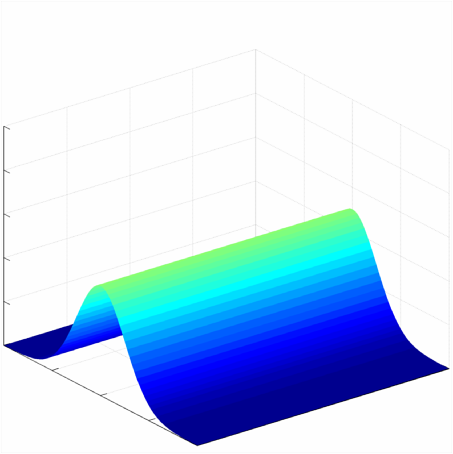
\includegraphics[width=0.2\textwidth]{\additivefigsdir/2d-kernel/additive_kernel_sum_p2} 
& \hspace{-0.4cm} \raisebox{1cm}{+} \hspace{-0.4cm} & 
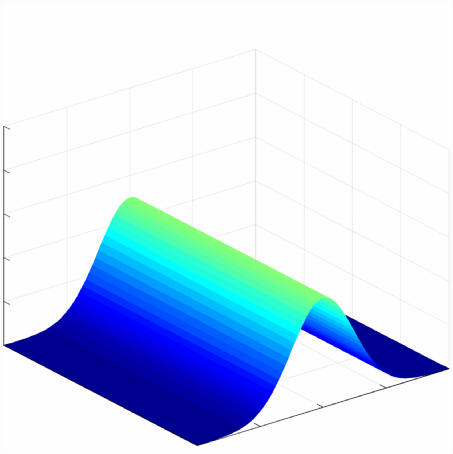
\includegraphics[width=0.2\textwidth]{\additivefigsdir/2d-kernel/additive_kernel_sum_p1} 
& \hspace{-0.4cm} \raisebox{1cm}{=} \hspace{-0.4cm} & 
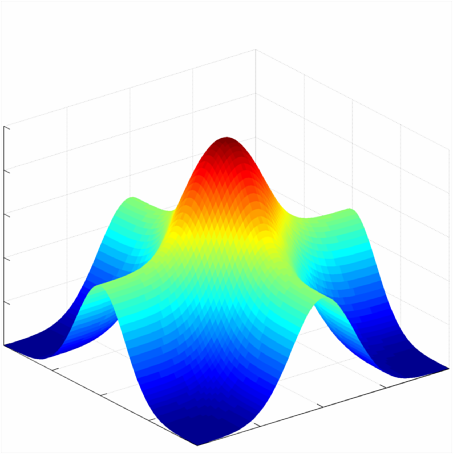
\includegraphics[width=0.2\textwidth]{\additivefigsdir/2d-kernel/additive_kernel} \\
$k_1(x_1, x_1')$ & & $k_2(x_2, x_2')$ & & $k_1(x_1,x_1') + k_2(x_2,x_2')$ \\[1em]
\large $\downarrow$ & & \large $\downarrow$ & & \large $\downarrow$ \\[-0.2em]
\hspace{-0.2cm}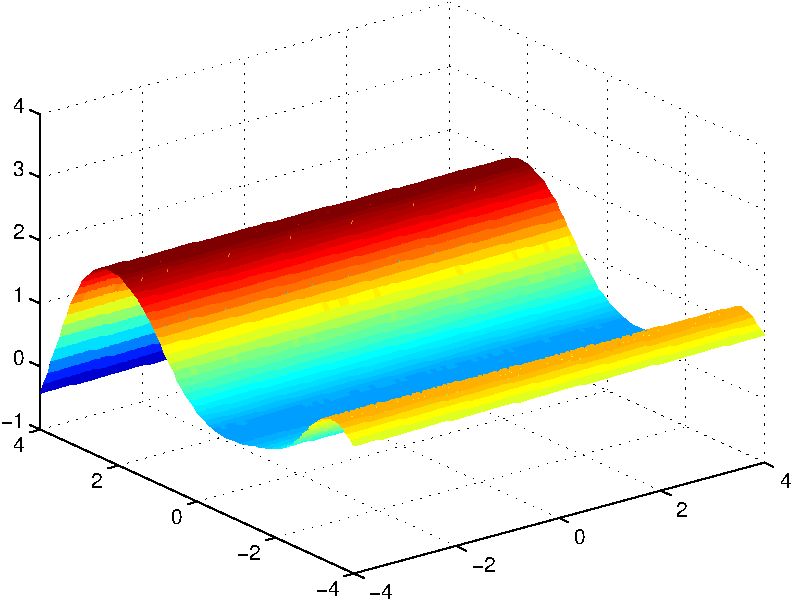
\includegraphics[width=0.2\textwidth]{\additivefigsdir/2d-kernel/additive_kernel_draw_sum_p1}
& \hspace{-0.4cm} \raisebox{1cm}{+} \hspace{-0.4cm} & 
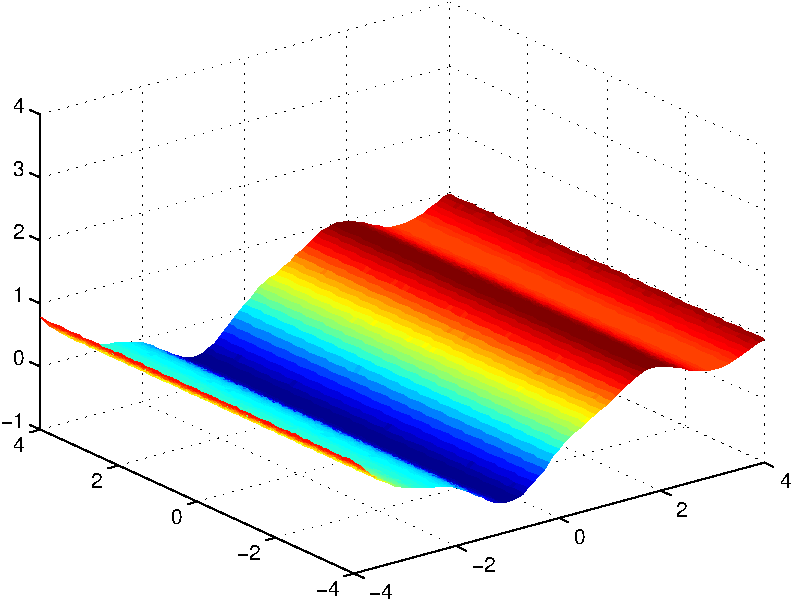
\includegraphics[width=0.2\textwidth]{\additivefigsdir/2d-kernel/additive_kernel_draw_sum_p2}
& \hspace{-0.4cm} \raisebox{1cm}{=} \hspace{-0.4cm} &
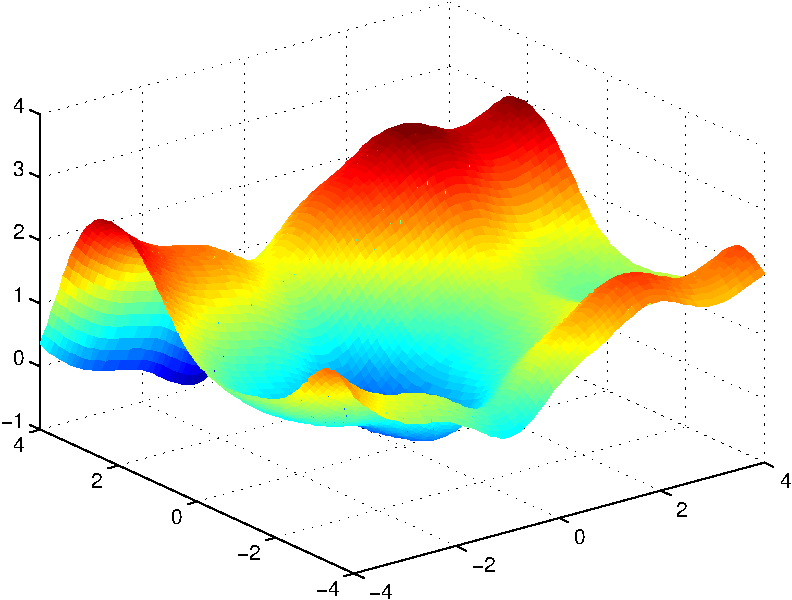
\includegraphics[width=0.2\textwidth]{\additivefigsdir/2d-kernel/additive_kernel_draw_sum} \\
$f_1(x_1) \sim \GP\left(0, k_1\right)$ & & $f_2(x_2) \sim \GP\left(0, k_2\right)$ & & $f_1(x_1) + f_2(x_2)$ \\[1em]
\end{tabular}
\caption[Additive kernels correspond to additive functions]{
A sum of two orthogonal one-dimensional kernels.
\emph{Top row:} An additive kernel is any sum of kernels.
\emph{Bottom row:} A draw from an additive kernel corresponds to a sum of draws from independent \gp{} priors, each having the corresponding kernel.
}
\label{fig:sum-of-kernels}
\end{figure}
%
For example, if
%
\begin{align}
%\function := 
f(x_1, x_2) \dist \GP(0, \kernel_1(x_1, x_1') + \kernel_2(x_2, x_2'))
\end{align}
%
Then this is equivalent to the model
%
\begin{align}
\function_1(x_1) & \dist \GP(0, \kernel_1(x_1, x_1'))\\
\function_2(x_2) & \dist \GP(0, \kernel_2(x_2, x_2'))\\
f(x_1, x_2) & = f_1(x_1) + f_2(x_2)
\end{align}
%
%Then we can model the sum of those functions through another \gp{}:
%

\Cref{fig:sum-of-kernels} illustrates a decomposition of this form.
Note that the product of two kernels does not have an analogous interpretation as the product of two functions.


\subsection{Long-range extrapolation through additivity}
\label{sec:additivity-extrapolation}

Additive structure often allows us to make predictions far from the training data.
%
\begin{figure}
\centering
\begin{tabular}{ccc}
 & \gp{} mean using & \gp{} mean using \\
True function: & sum of $\kSE$ kernels: & product of $\kSE$ kernels: \\
\parbox{0.33\columnwidth}{$f(x_1, x_2) = \sin(x_1) + \sin(x_2)$} & $k_1(x_1, x_1') \kernplus k_2(x_2, x_2')$ &  $k_1(x_1, x_1') \kerntimes k_2(x_2, x_2')$ \\[0.2em]
\hspace{-0.1in}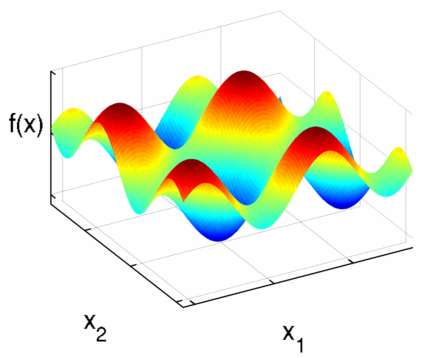
\includegraphics[width=0.32\textwidth]{\additivefigsdir/1st_order_censored_truth} &
\hspace{-0.1in}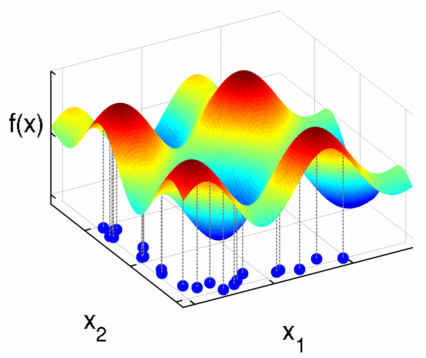
\includegraphics[width=0.32\textwidth]{\additivefigsdir/1st_order_censored_add} & 
\hspace{-0.1in}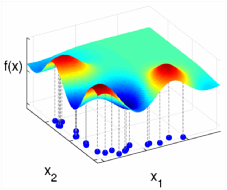
\includegraphics[width=0.32\textwidth]{\additivefigsdir/1st_order_censored_ard}\\[1em]
\end{tabular}
\caption[Long-range inference in functions with additive structure]
{\emph{Left:} A function with additive structure.
%Inference in functions with additive structure.
\emph{Center:} When the function being modeled has additive structure, a \gp{} with an additive kernel can exploit this fact to extrapolate far from the training data.
\emph{Right:} The product kernel allows a different function value for every combination of inputs, and so is uncertain about function values away from the training data.  This causes the predictions to revert to the mean.
%  The additive GP is able to discover the additive pattern, and use it to fill in a distant mode.  The ARD kernel can only interpolate, and thus predicts the mean in locations missing data.
}
\label{fig:synth2d}
\end{figure}
%
\Cref{fig:synth2d} compares the extrapolations made by additive versus product-kernel \gp{} models, conditioned on data from a sum of two axis-aligned sine functions.
The training data is confined to a small, L-shaped area.
In this example, the additive model is able to correctly predict the height of the function at unseen combinations of inputs.
The product-kernel model is more flexible, and so remains uncertain about the function away from the data.
%The ability of additive GPs to discover long-range structure suggests that this model may be well-suited to deal with covariate-shift problems.

These types of additive models have been well-explored in the statistics literature.
For example, generalized additive models~\citep{hastie1990generalized} have seen wide adoption.
In high dimensions, we can also consider sums of functions of more than one dimension.
\Cref{ch:additive} considers this model class in more detail.




\subsection{Example: an additive model of concrete strength}
\label{sec:concrete}

To illustrate how additive kernels give rise to interpretable models, we will build an additive model of the strength of concrete as a function of the amount of seven different ingredients, plus the age of the concrete \citep{yeh1998modeling}.
%We model measurements of the compressive strength of concrete, as a function of the concentration of 7 ingredients, plus the age of the concrete.

Our simple additive model looks like
%
\begin{align}
f(\vx) & = 
f_1(\textnormal{cement}) + f_2(\textnormal{slag}) + f_3(\textnormal{fly ash}) + f_4(\textnormal{water}) \nonumber \\
& \quad + f_5(\textnormal{plasticizer}) + f_6(\textnormal{coarse}) + f_7(\textnormal{fine}) + f_8(\textnormal{age}) + \textnormal{noise}
\label{eq:concrete}
\end{align}
%
where $\textnormal{noise} \simiid \Nt{0}{\sigma^2_n}$.
After learning the kernel parameters by maximizing the marginal likelihood of the data, we can visualize the predictive distribution of each component of the model.
%
%
\newcommand{\concretepic}[1]{\includegraphics[width=0.31\columnwidth]{\decompfigsdir/concrete-component-#1}}
\newcommand{\concretelegend}[0]{\raisebox{5mm}{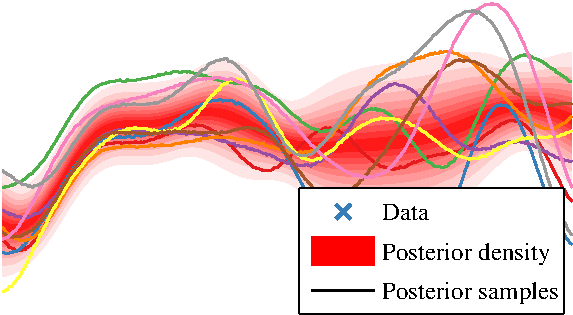
\includegraphics[trim=56mm 1mm 2mm 34.1mm, clip, width=0.24\columnwidth]{\decompfigsdir/concrete-component-8-legend}}}
%
\begin{figure}[h!]
\centering
\begin{tabular}{ccc}
%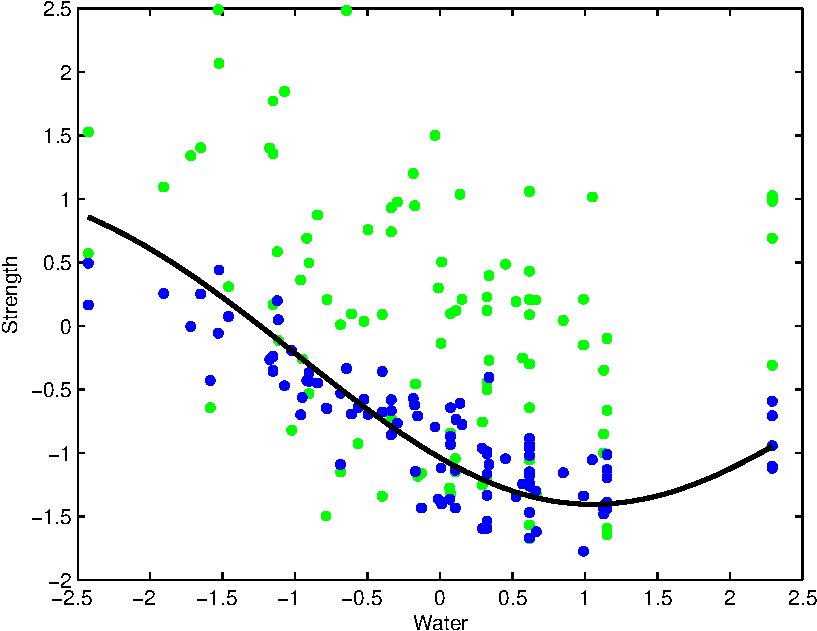
\includegraphics[width=0.3\textwidth]{\additivefigsdir/interpretable_1st_order1.pdf} &
%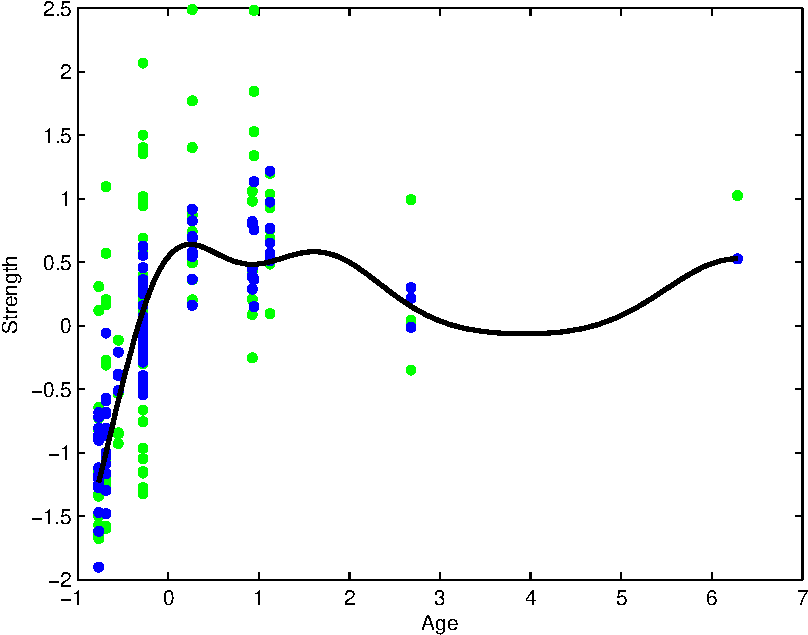
\includegraphics[width=0.3\textwidth]{\additivefigsdir/interpretable_1st_order2.pdf}& 
Cement & Slag & Fly Ash\\
\concretepic{1} & \concretepic{2} & \concretepic{3} \\
 Water & Plasticizer & Coarse\\
\concretepic{4} & \concretepic{5} & \concretepic{6} \\
 Fine & Age \\
 \concretepic{7} & \concretepic{8} & \concretelegend \\
\end{tabular}
\caption[Decomposition of posterior into interpretable one-dimensional functions]
{The predictive distribution of each component of a multidimensional additive model.
Blue crosses indicate the original data projected on to each dimension, red indicates the marginal posterior density, and colored lines are samples from the marginal posterior of each component.
The vertical axis is the same for all plots.
%The black line is the posterior mean of a \sgp{} with only one term in its kernel.
%Right:  the posterior mean of a \sgp{} with only one second-order term in its kernel.
%rs = 1 - var(complete_mean - y)/ var(y)
%R-squared = 0.9094
}
\label{fig:interpretable functions}
\end{figure}
%

\Cref{fig:interpretable functions} shows the marginal posterior distribution of each of the eight components in \cref{eq:concrete}.
We can see that the parameters controlling the variance of two of the components, Coarse and Fine, were set to zero, meaning that the marginal likelihood preferred a parsimonious model which did not depend on these dimensions.
This is an example of the automatic sparsity that arises by maximizing marginal likelihood in \gp{} models, and another example of automatic relevance determination (\ARD) \citep{neal1995bayesian}.

The ability to learn kernel parameters in this way is much more difficult when using non-probabilistic methods such as Support Vector Machines \citep{cortes1995support}, for which cross-validation is often the best method to select kernel parameters.



\subsection{Posterior variance of additive components}
\label{sec:posterior-variance}


%\footnote{Code is available at \url{github.com/duvenaud/phd-thesis/}}
Here we derive the posterior variance and covariance of all of the additive components of a \gp{}.
These formulas allow us to make plots such as \cref{fig:interpretable functions}.
%These formulas let us plot the marginal variance of each component separately.  These formulas can also be used to examine the posterior covariance between pairs of components.

First, we will write down the joint prior over the sum of two functions drawn from \gp{} priors.
We distinguish between $\vecf(\vX)$ (the function values at the training locations) and  $\vecf(\vX^\star)$ (the function values at some set of query locations).
% so that it's clear which matrices to use to extrapolate.

If $f_1$ and $f_2$ are \emph{a priori} independent, and $f_1 \sim \gp( \mu_1, k_1)$ and $f_2 \sim \gp( \mu_2, k_2)$, then
%
\begin{align}
\left[ \begin{array}{l} 
\vf_1(\vX) \\
\vf_1(\vX^\star) \\
\vf_2(\vX) \\
\vf_2(\vX^\star) \\
\vf_1(\vX) + \vf_2(\vX) \\
\vf_1(\vX^\star) + \vf_2(\vX^\star)
\end{array} \right]
\sim
\Nt{
\left[ \begin{array}{c} \vmu_1 \\ \vmu_1^\star \\ \vmu_2 \\ \vmu_2^\star \\ \vmu_1 + \vmu_2 \\ \vmu_1^\star + \vmu_2^\star \end{array} \right]
}
{\left[ \begin{array}{cccccc} 
\vK_1 & \vK_1^\star & 0 & 0 & \vK_1 & \vK_1^\star \\ 
\vK_1^\star & \vK_1^{\star\star} & 0 & 0 & \vK_1^\star & \vK_1^{\star\star} \\
0 & 0 & \vK_2 & \vK_2^\star & \vK_2 & \vK_2^\star \\ 
0 & 0 & \vK_2^\star & \vK_2^{\star\star} & \vK_2^\star & \vK_2^{\star\star} \\
\vK_1 & \vK_1^\star & \vK_2 & \vK_2^\star & \vK_1 + \vK_2 & \vK_1^\star + \vK_2^\star \\ 
\vK_1^\star & \vK_1^{\star\star}  & \vK_2^\star & \vK_2^{\star\star}  & \vK_1^\star + \vK_2^\star & \vK_1^{\star\star} + \vK_2^{\star\star}\\
\end{array} \right]
}
\end{align}
%
where we represent the Gram matrices, evaluated at all pairs of vectors in bold capitals as ${\vK_{i,j} = k(\vx_i, \vx_j)}$.  So 
%
\begin{align}
\vK_1 & = k_1( \vX, \vX ) \\
\vK_1^\star & = k_1( \vX^\star, \vX ) \\
\vK_1^{\star\star} & = k_1( \vX^\star, \vX^\star )
\end{align}

By the formula for Gaussian conditionals, (given by \cref{eq:gauss_conditional}), we get that the conditional distribution of a \gp{}-distributed function conditioned on its sum with another \gp{}-distributed function is given by
%
\begin{align}
\vf_1(\vX^\star) | \vf_1(\vX) + \vf_2(\vX) \sim \Normal \Big( 
& \vmu_1^\star + \vK_1^{\star\tra} (\vK_1 + \vK_2)\inv \left[ \vf_1(\vX) + \vf_2(\vX) - \vmu_1 - \vmu_2 \right] \nonumber \\
& \vK_1^{\star\star} - \vK_1^{\star\tra} (\vK_1 + \vK_2)\inv \vK_1^{\star} \Big)
%\vf_1(\vx^\star) | \vf(\vx) \sim \mathcal{N}\big( 
%& \vmu_1(\vx^\star) + \vk_1(\vx^{\star}, \vx)  \left[ \vK_1(\vx, \vx) + \vK_2(\vx, \vx) \right]\inv \left( \vf(\vx) - \vmu_1(\vx) - \vmu_2(\vx) \right) , \nonumber \\
%& \vk_1(\vx^{\star}, \vx^{\star}) - \vk_1(\vx^{\star}, \vx)  \left[ \vK_1(\vx, \vx) + \vK_2(\vx, \vx) \right] \inv \vk_1(\vx, \vx^{\star}) 
%\big).
\end{align}
%
These formulas express the model's posterior uncertainty about the different components of the signal, integrating over the possible configurations of the other components.
To extend these formulas to a sum of more than two functions, the term $\vK_1 + \vK_2$ can simply be replaced by $\sum_i \vK_i$ everywhere.




\subsubsection{Posterior covariance of additive components}

%One of the advantages of using a generative, model-based approach is that we can examine any aspect of the model we wish to.
We can also compute the posterior covariance between any two components, conditioned on their sum:
if this quantity is negative, it means that there is ambiguity about which of the two components explains the data at that location.
\begin{figure}
\centering
\renewcommand{\tabcolsep}{1mm}
\def\incpic#1{\includegraphics[width=0.1\columnwidth]{../figures/decomp/concrete-#1}}
\begin{tabular}{p{2mm}*{6}{c}}
 & {Cement} & {Slag} & {Fly Ash} & {Water} & \parbox{0.1\columnwidth}{Plasticizer} & {Age} \\ 
 \rotatebox{90}{{Cement}} & \incpic{Cement-Cement} & \incpic{Cement-Slag} & \incpic{Cement-Fly-Ash} & \incpic{Cement-Water} & \incpic{Cement-Plasticizer} & \incpic{Cement-Age} \\ 
 \rotatebox{90}{{Slag}} & \incpic{Slag-Cement} & \incpic{Slag-Slag} & \incpic{Slag-Fly-Ash} & \incpic{Slag-Water} & \incpic{Slag-Plasticizer} & \incpic{Slag-Age} \\ 
 \rotatebox{90}{{Fly Ash}} & \incpic{Fly-Ash-Cement} & \incpic{Fly-Ash-Slag} & \incpic{Fly-Ash-Fly-Ash} & \incpic{Fly-Ash-Water} & \incpic{Fly-Ash-Plasticizer} & \incpic{Fly-Ash-Age} \\ 
 \rotatebox{90}{{$\quad$Water}} & \incpic{Water-Cement} & \incpic{Water-Slag} & \incpic{Water-Fly-Ash} & \incpic{Water-Water} & \incpic{Water-Plasticizer} & \incpic{Water-Age} \\ 
 \rotatebox{90}{\parbox{0.1\columnwidth}{Plasticizer}} & \incpic{Plasticizer-Cement} & \incpic{Plasticizer-Slag} & \incpic{Plasticizer-Fly-Ash} & \incpic{Plasticizer-Water} & \incpic{Plasticizer-Plasticizer} & \incpic{Plasticizer-Age} \\ 
 \rotatebox{90}{{Age}} & \incpic{Age-Cement} & \incpic{Age-Slag} & \incpic{Age-Fly-Ash} & \incpic{Age-Water} & \incpic{Age-Plasticizer} & \incpic{Age-Age} \\
 \end{tabular}
 \fbox{
\begin{tabular}{c}
 Correlation \\[1ex]
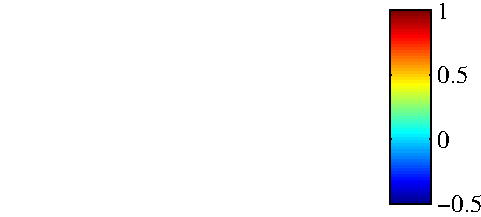
\includegraphics[width=0.1\columnwidth, clip, trim=6.2cm 0cm 0cm 0cm]{../figures/decomp/concrete-colorbar}
\end{tabular}
}
\caption[Visualizing posterior correlations between components]
{Posterior correlations between the components explaining the concrete dataset.
Each plot shows the additive model's posterior correlations between two components, plotted over the domain of the data $\pm 5\%$.
%Color indicates the amount of correlation between the function value of the two components.
Red indicates high correlation, teal indicates no correlation, and blue indicates negative correlation.
Plots on the diagonal show posterior correlations within each component.
%Off-diagonal plots show posterior covariance between each pair of functions, as a function of both inputs.
%Negative correlation means that one function is high and the other low, but which one is uncertain.
Dimensions `Coarse' and `Fine' are not shown, because their variance is zero.
}
\label{fig:interpretable interactions}
\end{figure}
%
%
\begin{align}
\covargs{ \vf_1(\vX^\star)}{\vf_2(\vX^\star) | \vf(\vX) } 
& = - \vK_1^{\star\tra} (\vK_1 + \vK_2)\inv \vK_2^\star
%\covargs{\vf_1(\vx^\star)}{\vf_2(\vx^\star) | \vf(\vx) }
%& = - \vk_1(\vx^{\star}, \vx)  \left[ \vK_1(\vx, \vx) + \vK_2(\vx, \vx) \right] \inv \vk_1(\vx, \vx^{\star}) 
\label{eq:post-component-cov}
\end{align}
%
\Cref{fig:interpretable interactions} shows the posterior correlation between all non-zero components of the concrete model.
Most of the correlation occurs within components, but there is also negative correlation between the ``Cement'' and ``Slag'' variables.
This reflects an ambiguity in the model about which one of these functions is high and the other low.






\section{Changepoints}
\label{sec:changepoint-definition}
A simple example of how combining kernels can give rise to more structured priors is given by changepoint kernels.
Changepoints kernels can be defined through addition and multiplication with sigmoidal functions such as $\sigma(x) = \nicefrac{1}{1 + \exp(-x)}$:
%
\begin{align}
%\kCP(\kernel_1, \kernel_2) = \kernel_1 \kerntimes \boldsymbol\sigma \kernplus \kernel_2 \kerntimes \boldsymbol{\bar\sigma}
%\kCP(\kernel_1, \kernel_2) & = \begin{array}{rl} (1-\sigma(x)) & k_2(x,x')(1-\sigma(x')) \\
%  + \sigma(x) & k_1(x,x')\sigma(x') \end{array} \\
\kCP(\kernel_1, \kernel_2)(x,x') & = \sigma(x) k_1(x,x')\sigma(x') + (1-\sigma(x)) k_2(x,x')(1-\sigma(x'))
\label{eq:cp}
\end{align}
%
which can be written in shorthand as
%
\begin{align}
\kCP(\kernel_1, \kernel_2)& = \kernel_1 \kerntimes \boldsymbol\sigma \kernplus \kernel_2 \kerntimes \boldsymbol{\bar\sigma}
\end{align}
where $\boldsymbol\sigma = \sigma(x)\sigma(x')$ and $\boldsymbol{\bar\sigma} = (1-\sigma(x))(1-\sigma(x'))$.

This compound kernel expresses a change from one kernel to another.
The parameters of the sigmoid determine where, and how rapidly, this change occurs.

\newcommand{\cppic}[1]{\includegraphics[height=2.2cm,width=3.3cm]{\grammarfiguresdir/changepoint/#1}}%
\begin{figure}[h]
\centering
\begin{tabular}{rcccc}
 & $\kCP(\kSE, \kPer)$ & $\kCP(\kSE, \kPer)$ & $\kCP(\kSE, \kSE)$ & $\kCP(\kPer, \kPer)$ \\
\raisebox{1cm}{f(x)} \hspace{-0.4cm} & \cppic{draw_1} & \cppic{draw_2} & \cppic{draw_3} & \cppic{draw_4} \\
& $x$ & $x$ & $x$ & $x$
\end{tabular}
\caption[Draws from changepoint priors]
{Draws from different priors on using changepoint kernels, constructed by adding and multiplying together base kernels with sigmoidal functions.
}
\label{fig:changepoint_examples}
\end{figure}

We can also express a function whose structure changes within some interval -- a \emph{change window} -- by replacing $\sigma(x)$ with a product of two sigmoids, one increasing and one decreasing.

\subsection{Multiplication by a known function}

More generally, we can model an unknown function that's been multiplied by some fixed, known function $a(x)$, by multiplying the kernel by $a(\vx) a(\vx')$.
Formally,
%
\begin{align}
f(\iva) = a(\iva) g(\iva), \quad g \sim \GPdist{g}{\vzero}{k(\iva, \iva')} \quad
\iff
\quad f \sim \GPdist{f}{\vzero}{ a(\iva) k(\iva, \iva') a(\iva')}
\end{align}




\section{Feature representation of kernels}
%
By Mercer's theorem \citep{mercer1909functions},
%Due to \citet{mercer1909functions}, we know that
any positive-definite kernel can be represented as the inner product between a fixed set of features, evaluated at $\vx$ and at $\vx'$:
%
\begin{align}
k(\vx, \vx') = \feat(\vx)\tra \feat(\vx')
\end{align}

As a simple example, the squared-exponential kernel ($\kSE$) on the real line has a representation in terms of infinitely many radial-basis functions of the form ${h_i(x) \propto \exp( -\frac{1}{2} \frac{(x - c_i)^2}{2\ell^2})}$.
More generally, any stationary kernel
% (one which only depends on the distance between its inputs) 
on the real line can be represented by a set of sines and cosines - a Fourier representation \citep{bochner1959lectures}.
In general, any particular feature representation of a kernel is not unique, and depends on which space $\InputSpace$ is being considered \citep{minh2006mercer}.

In some cases, $\InputSpace$ can even be the infinite-dimensional feature mapping of another kernel.  Composing feature maps in this way leads to \emph{deep kernels}, a topic explored in \cref{ch:deep-limits}.



\subsection{Relation to linear regression}

Surprisingly, \gp{} regression is equivalent to Bayesian linear regression on the implicit features $\feat(\vx)$ which give rise to the kernel:
%
\begin{align}
f(\iva) = \vw\tra \feat(\iva), \quad \vw \sim \N{\vw}{\vzero}{\vI} \quad
\iff
\quad f \sim \GPdist{f}{\vzero}{\feat(\iva) \tra \feat(\iva)}
\end{align}
%
The link between Gaussian processes, linear regression, and neural networks is explored further in \cref{ch:deep-limits}.


\subsection{Feature-space view of combining kernels}

\def\feata{\va}
\def\featb{\vb}

%Many architectures for learning complex functions, such as convolutional networks \cite{lecun1989backpropagation} and sum-product networks \cite{poon2011sum}, include units which compute \texttt{and}-like and \texttt{or}-like operations.
%Composite kernels can be viewed in this way too.
%A sum of kernels can be understood as an \texttt{or}-like operation: two points are considered similar if either kernel has a high value.
%Similarly, multiplying kernels is an \texttt{and}-like operation, since two points are considered similar only if both kernels have high values.


We can also view kernel addition and multiplication as a combination of the features of the original kernels.
%Viewing kernel addition from this point of view, if
For example, if we have two kernels
%
\begin{align}
k_a(\iva, \iva') & = \feata(\iva)\tra \feata(\iva')\\
k_b(\iva, \iva') & = \featb(\iva)\tra \featb(\iva')
\end{align}
%
then their addition has the form:
%
\begin{align}
k_a(\iva, \iva') + k_b(\iva, \iva')
& = \feata(\iva)\tra \featb(\iva') + \feata(\iva)\tra \featb(\iva') 
 = \colvec{\feata(\iva)}{\featb(\iva)}\tra \colvec{\feata(\iva')}{\featb(\iva')}
\end{align}
%
meaning that the features of $k_a + k_b$ are the concatenation of the features of each kernel.

We can examine kernel multiplication in a similar way:
%
\begin{align}
k_a(\iva, \iva') \times k_b(\iva, \iva')
& = \left[ \feata(\iva)\tra \feata(\iva') \right] \times \left[ \featb(\iva)\tra \featb(\iva') \right] \\
%& = \left[ \begin{array}{c} \feat_1(\iva) \\ \feat_2(\iva) \end{array} \right]^\tra \left[ \begin{array}{c} \feat_1(\iva') \\ \feat_2(\iva') \end{array} \right]
& = \sum_i a_i(\iva) a_i(\iva') \times \sum_j b_j(\iva) b_j(\iva') \\
%& = \sum_i \sum_j a_i(\iva) a_i(\iva') b_j(\iva) b_j(\iva') \\
& = \sum_{i,j} \big[ a_i(\iva) b_j(\iva) \big] \big[ a_i(\iva') b_j(\iva') \big] \\
& = \vecop{ \feata(\iva) \otimes \featb(\iva') } \tra \vecop{ \feata(\iva) \otimes \featb(\iva')} 
\end{align}
%
In other words, the features of $k_a \times k_b$ are just the Cartesian product (all possible combinations) of the original two sets of features.
For example, the Cartesian product of the features of two one-dimensional $\kSE$ kernels covers the plane with two-dimensional radial-basis functions of the form
%
\begin{align}
h_{ij}(x_1, x_2) \propto \exp \left( -\frac{1}{2} \frac{(x_1 - c_i)^2}{2\ell_1^2} \right) \exp \left( -\frac{1}{2} \frac{(x_2 - c_j)^2}{2\ell_2^2} \right)
\end{align}





\section{Expressing symmetries and invariants}
\label{sec:expressing-symmetries}

\def\gswitch{G_\textnormal{swap}}

When modeling functions, encoding known symmetries can improve predictive accuracy. 
This section looks at different ways to encode symmetries into a prior on functions.
Many types of symmetry can be enforced through operations on the kernel.

We will demonstrate the properties of the resulting models by sampling functions from their priors.
By using these functions to define warpings from $\Reals^2 \to \Reals^3$, we will show how to build a nonparametric prior on an open-ended family of topological manifolds, such as cylinders, toruses, and M\"{o}bius strips.

\subsection{Three recipes for invariant priors}

Consider the scenario where we have a finite set of transformations of the input space $\{g_1, g_2, \ldots \}$ to which we wish our function to remain invariant:
%
\begin{align}
f(\vx) = f(g(\vx))  \quad \forall \vx \in \mathcal{X}, \quad \forall g \in G
\end{align}
%
As an example, imagine we want to build a model of functions invariant to swapping their inputs: $f(x_1, x_2) = f(x_2, x_1)$.
Being invariant to a set of operations is equivalent to being invariant to all compositions of those operations, the set of which form a group. \citep[chapter 21]{armstrong1988groups}.
In our example, the elements of the group $\gswitch$ containing the operations the functions are invariant to has two elements:%, and is an example of the symmetric group $S2$:
%
\begin{align}
g_1([x_1, x_2]) & = [x_2, x_1] \qquad \textnormal{(swap)} \\
g_2([x_1, x_2]) & = [x_1, x_2] \qquad \textnormal{(identity)}
\end{align}
%
How can we construct a prior on functions which respect these symmetries?

\citet{ginsbourger2012argumentwise} and \citet{Invariances13} showed that the only way to construct a \gp{} prior on functions which respect a set of invariants is to construct a kernel which respects the same invariants with respect to each of its two inputs:
%
\begin{align}
k(\vx, \vx') = k( g(\vx), g(\vx')), \quad \forall \vx, \vx' \in \InputSpace, \quad \forall g, g' \in G
\end{align}
%
Formally, given a finite group $G$ whose elements are operations to which we wish our function to remain invariant, and $f \sim \GPt{0}{k(\vx,\vx')}$, then every $f$ is invariant under $G$ (up to a modification) if and only if $k(\cdot, \cdot)$ is argument-wise invariant under $G$.

It might not always be clear how to construct a kernel respecting such argument-wise invariances.
%Fortunately, for finite groups, there are a few simple ways to transform any kernel into one which is argument-wise invariant to actions under any finite group:
Fortunately, there are a few simple ways to do this for any finite group:
%
%
\begin{figure}
\renewcommand{\tabcolsep}{1.5mm}
\begin{tabular}{ccc}
Additive method & Projection method & Product method \\[0.5ex]
\includegraphics[width=0.3\columnwidth]{\symmetryfigsdir/symmetric-xy-naive-sample} &
\includegraphics[width=0.3\columnwidth]{\symmetryfigsdir/symmetric-xy-projection-sample} &
\includegraphics[width=0.3\columnwidth]{\symmetryfigsdir/symmetric-xy-prod-sample}\\
%$k(x, y, x', y') + k(x, y, y', x')$ & $k(x, y, x', y') \times k(x, y, y', x')$ & $k( \min(x, y), \max(x,y),$ \\
% $+ k(y, x, x', y') + k(y, x, y', x')$ & $\times k(y, x, x', y') \times k(y, x, y', x')$ & $\min(x', y'), \max(x',y') )$
$\begin{array}{r@{}l@{}}
& \kSE(x_1, x_2, x_1', x_2') \\ + \,\, & \kSE(x_1, x_2, x_2', x_1')
\end{array}$
&
$\begin{array}{r@{}l@{}}
\kSE( \!\! &{}\min(x_1, x_2), \max(x_1, x_2), \\
           &{}\min(x_1', x_2'), \max(x_1',x_2') )
\end{array}$
&
$\begin{array}{r@{}l@{}}
& \kSE(x_1, x_2, x_1', x_2') \\ \times \,\, & \kSE(x_1, x_2, x_2', x_1')
\end{array}$
\end{tabular}
\caption[Three ways to introduce symmetry]{Three methods of introducing symmetry, illustrated through draws from the corresponding priors.
%Left:  The additive method.
%Center: The product method.
%Right: The projection method.
%The additive method has half the marginal variance away from $y = x$, but the min method introduces a non-differentiable seam along $y = x$.
All three methods introduce a different type of nonstationarity.
}
\label{fig:add_vs_min}
\end{figure}
%
\begin{enumerate}

\item {\bf Sum over the orbit.} 
\citet{ginsbourger2012argumentwise} and \citet{kondor2008group} suggest enforcing invariants through a double sum over the orbits of $\vx$ and $\vx'$ with respect to G:
%
\begin{align}
k_\textnormal{sum}(\vx, \vx') = \sum_{g, \in G} \sum_{g' \in G} k( g( \vx ), g'( \vx') )
\end{align}

For the group $\gswitch$, this operation results in the kernel:
%
\begin{align}
k_\textnormal{switch}(\vx, \vx')
& = \sum_{g \in \gswitch} \sum_{g' \in \gswitch} k( g( \vx ), g'( \vx') ) \\
& = k(x_1, x_2, x_1', x_2') + k(x_1, x_2, x_2', x_1')  \nonumber \\ 
& \quad + k(x_2, x_1, x_1', x_2') + k(x_2, x_1, x_2', x_1')
\end{align}
%
For stationary kernels, some pairs of elements in this sum will be identical, and can be ignored.
\Cref{fig:add_vs_min}(left) shows a draw from a \gp{} prior with an $\kSE$ kernel symmetrized in this way.
This construction has the property that the marginal variance is doubled near $x = y$, which may or may not be desirable.



\item {\bf Project onto a fundamental domain.}
\citet{Invariances13} also explore the possibility of projecting each datapoint into a fundamental domain of the group, using a mapping $A_G$:
%
\begin{align}
k_\textnormal{proj}(\vx, \vx') = k( A_G(\vx), A_G( \vx') )
\end{align}
%
For the group $\gswitch$, a fundamental domain is $\{x_1, x_2 : x_1 < x_2\}$, which can be mapped to using $A_{\gswitch}( x_1, x_2 ) = \big[ \min(x_1, x_2), \max(x_1, x_2) \big]$.
Constructing a kernel using this method introduces a non-differentiable  ``seam'' along $x_1 = x_2$, as shown in \cref{fig:add_vs_min}(center).
%The projection method also works for infinite groups, as we shall see below.

\item {\bf Multiply over the orbit.}
%\citet{adams2013product}
Ryan Adams (personal communication) suggested a construction enforcing invariants through products over the orbits:
%
\begin{align}
k_\textnormal{sum}(\vx, \vx') = \prod_{g \in G} \prod_{g' \in G} k( g( \vx ), g'( \vx') )
\end{align}
%
This method can sometimes produce \gp{} priors with zero variance in some regions of the space, as in \cref{fig:add_vs_min}(right).
%We include it here to show that each of these methods for enforcing symmetries modifies the resulting model in other ways as well.
\end{enumerate}
%
There are many possible ways to achieve a given symmetry, but we must be careful to do so without compromising other qualities of the model we are constructing.
For example, simply setting $k(\vx, \vx') = 0$ gives rise to a \gp{} prior which obeys \emph{all possible} symmetries, but this is presumably not a model we wish to use.




%In this section, we give recipes for expressing several classes of symmetries.  Later, we will show how these can be combined to produce more interesting structures.


\subsection{Example: periodicity}

%We can enforce periodicity on any subset of the dimensions:
Periodicity in a one-dimensional function corresponds to the invariance
%
\begin{align}
f(x) = f( x + \tau)
\label{eq:periodic_invariance}
\end{align}
%
where $\tau$ is the period.

The most popular method for building a periodic kernel is due to \citet{mackay1998introduction}, who used the projection method in combination with an $\kSE$ kernel.
A fundamental domain of the symmetry group is a circle, so the kernel
%
%The representer transformation for periodicity is simply $A(x) = [\sin(x), \cos(x)]$:
%
\begin{align}
\kPer(x, x') = \kSE \left( \big[ \sin(x), \cos(x) \big], \big[ \sin(x'), \cos(x') \big] \right)
\end{align}
%
%We can also apply rotational symmetry repeatedy to a single dimension.
achieves the invariance in \cref{eq:periodic_invariance}.
Simple algebra reduces this kernel to the form shown in \cref{fig:basic_kernels}.

We could also build a periodic kernel with period $\tau$ by the mapping $A(x) = \mod(x, \tau)$.
However, samples from this prior would be discontinuous at every integer multiple of $\tau$.

\subsection{Example: symmetry about zero}

Another simple example of an easily-enforceable symmetry is symmetry about zero:
%
\begin{align}
f(x) = f( -x)
\end{align}
%
using the sum over orbits method, by the transform
%
\begin{align}
k_{\textnormal{reflect}}(x, x') & = k(x, x') + k(x, -x') + k(-x, x') + k(-x, -x')
\end{align}

%This transformation can be applied to any subset of dimensions

%\paragraph{Spherical Symmetry}

%We can also enforce that a function expresses the symmetries obeyed by $n-spheres$ by simply transforming a set of $n - 1$ coordinates by:
%
%\begin{align}
%x_1 & = \cos(\phi_1) \nonumber \\
%x_2 & = \sin(\phi_1) \cos(\phi_2) \nonumber \\
%x_3 & = \sin(\phi_1) \sin(\phi_2) \cos(\phi_3) \nonumber \\
%& \vdots \nonumber \\
%x_{n-1} & = \sin(\phi_1) \cdots \sin(\phi_{n-2}) \cos(\phi_{n-1}) \nonumber \\
%x_n & = \sin(\phi_1) \cdots \sin(\phi_{n-2}) \sin(\phi_{n-1})
%\end{align}

%\cite{flanders1989}



\subsection{Example: translation invariance in images}

Most models of images are invariant to spatial translations \citep{lecun1995convolutional}.
Similarly, most models of sounds are also invariant to translation through time.

This sort of translation invariance is completely distinct from the stationarity of kernels such as $\kSE$ or $\kPer$.
A stationary kernel implies that the prior is invariant to translations of the entire training and test set.
In contrast, we use translation invariance to refer to the situation where the signal has been discretized, and each pixel (or the audio equivalent) corresponds to a different input dimension.
We are interested in creating priors on functions that are invariant to swapping pixels in a manner that corresponds to shifting in some direction:
%
\begin{align}
f \Bigg( \raisebox{-2.5ex}{ \includegraphics[width=1cm]{\topologyfiguresdir/grid2} } \Bigg) 
= f \Bigg( \raisebox{-2.5ex}{ \includegraphics[width=1cm]{\topologyfiguresdir/grid3} } \Bigg)
\end{align}
%
%In this setting, translation is equivalent to swapping dimensions of the input vector $\vx$.
For example, in a one-dimensional image or audio signal, translation of an input vector by $i$ pixels can be defined as
%
\begin{align}
\shift(\vx, i) = \big[ x_{\mod( i + 1, D )}, x_{\mod( i + 2, D )}, \dots, x_{\mod( i + D, D )} \big]\tra
\end{align}
%
As above, translation invariance in one dimension can be achieved by the transformation
%
\begin{align}
%k \left( (x_1, x_2, \dots, x_D ), (x_1', x_2', \dots, x_D' ) \right) & = %\nonumber \\
%\sum_{i=1}^D \prod_{j=1}^D k( x_j, x_{ i + j \textnormal{mod $D$} }' )
k_\textnormal{invariant} \left( \vx, \vx' \right) = %\nonumber \\
\sum_{i=1}^D \sum_{j=1}^D k( \shift(\vx, i), \shift(\vx, j) ) \,,
\end{align}
%
simply defining the covariance between two signals to be the sum of all covariances between all translations of those two signals.

The extension to two dimensions, $\shift(\vx, i, j)$, is straightforward, but notationally cumbersome.
\citet{kondor2008group} built a more elaborate kernel between images, approximately invariant to both translation and rotation by using the projection method.

%Is there a pathology of the additive construction that appears in the limit?

%\subsection{Max-pooling}
%What we'd really like to do is a max-pooling operation.  However, in general, a kernel which is the max of other kernels is not PSD [put counterexample here?].  Is the max over co-ordinate switching PSD?





\section{Generating topological manifolds}
\label{sec:topological-manifolds}

In this section we give a geometric illustration of the symmetries encoded by different compositions of kernels.
The work presented in this section is based on a collaboration with David Reshef, Roger Grosse, Joshua B. Tenenbaum, and Zoubin Ghahramani.
The derivation of the M\"obius kernel was an original contribution by myself.

Priors on functions exhibiting symmetries can be used to create a prior on topological manifolds, by warping a simply-connected surface into a higher-dimensional space using a mapping expressing symmetries. %from a latent space to an observed space.%surface $f(\vx)$.
%The distribution on $\vf$ allows us to put mass on 
%If we set the input $\vx$ to be a 2-dimensional plane, intro 3 dimensions using a \gp{} encoding certain symmetries, the resulting surfaces will correspon
To build a prior on 2-dimensional manifolds embedded in 3-dimensional space, we simply need a prior on mappings from $\mathbb{R}^2$ to $\mathbb{R}^3$, which we can construct using three independent functions $[f_1(\vx), f_2(\vx), f_3(\vx)]$, each mapping from $\mathbb{R}^2$ to $\mathbb{R}$.
\gp{} priors on the mapping functions implictly give rise to a prior on warped surfaces.
Symmetries in $[f_1, f_2, f_3]$ will connect different parts of the manifolds, giving rise to non-trivial topologies on the sampled surfaces.
%
\begin{figure}
\renewcommand{\tabcolsep}{1mm}
\begin{tabular}{ccc}
Euclidian $( \SE_1 \times \SE_2 )$  & Cylinder $( \SE_1 \times \Per_2 )$ & Toroid $( \Per_1 \times \Per_2 )$\\
\hspace{-0.5cm}\includegraphics[width=0.33\columnwidth,clip=true,trim=10mm 10mm 1mm 1mm]{\topologyfiguresdir/manifold} &
\includegraphics[width=0.33\columnwidth,clip=true,trim=10mm 10mm 10mm 10mm]{\topologyfiguresdir/cylinder} &
\includegraphics[width=0.33\columnwidth,clip=true,trim=1mm 1mm 1mm 1mm]{\topologyfiguresdir/torus} \\
\end{tabular}
\caption[Generating 2D manifolds with different topological structures]{
Generating 2D manifolds with different topologies.
By enforcing that the functions mapping from $\mathbb{R}^2$ to $\mathbb{R}^3$ obey the appropriate symmetries, the surfaces created have the corresponding topologies, ignoring self-intersections.
}
\label{fig:gen_surf}
\end{figure}
%
\Cref{fig:gen_surf} shows 2D meshes warped into 3D by functions drawn from \gp{} priors with different kernels, giving rise to a variety of different topologies.
%
Higher-dimensional analogues of these shapes can be constructed by increasing the latent dimension and including corresponding terms in the kernel.
For example, an $N$-dimensional space with kernel $\kPer_1 \kerntimes \kPer_2 \kerntimes \ldots \kerntimes \kPer_N$ will give rise to a prior on $N$-dimensional toruses.

This construction is similar in spirit to the \gp{} latent variable model (\gplvm{}) of \citet{lawrence2005probabilistic}, which learns a latent embedding of the data into a low-dimensional space, using a \gp{} prior on the mapping from the latent space to the observed space.



\subsection{M\"{o}bius strips}

A prior on functions on M\"{o}bius strips can be constructed by enforcing the symmetries:
%
\begin{align}
f(x_1, x_2) & = f( x_1 + \tau, x_2) \qquad \textnormal{(periodic in $x_1$)} \nonumber \\
f(x_1, x_2) & = f( x_1, x_2 + \tau) \qquad \textnormal{(periodic in $x_1$)} \nonumber \\
f(x_1, x_2) & = f( x_2, x_1)  \quad \,\,\,\;     \qquad \textnormal{(symmetric about $x_1 = x_2$)} \nonumber 
\end{align}
%
We'll call a kernel which enforces these symmetries a \emph{M\"{o}bius kernel}:
%
\begin{align}
k(x_1, x_2, x_1', x_2') = 
\Per(x_1, x_1') \kerntimes \Per(x_2, x_2') \kernplus
\Per(x_1, x_2') \kerntimes \Per(x_2, x_1')
\end{align}
%
Moving along the diagonal $x_1 = x_2$ of a function drawn from the corresponding \gp{} prior is equivalent to moving along the edge of a notional M\"{o}bius strip which has had the function mapped on to its surface.
\Cref{fig:mobius}(a) shows an example of a function drawn from such a prior.
%
\begin{figure}
\begin{tabular}[t]{ccc}
%\begin{columns}
\centering
Draw from \gp{} with kernel: &  &  \\
%$( \Per_1 \times \Per_2 )$ and $f(x,y) = f(y,x)$ & generated parametrically\\
$\begin{array}{l@{}l@{}}
&            \Per(x_1, x_1') \kerntimes \Per(x_2, x_2') \\
 \kernplus & \Per(x_1, x_2') \kerntimes \Per(x_2, x_1')
\end{array}$
& $\begin{array}{c} \textnormal{ M\"{o}bius strip drawn from}  \\ \textnormal{$\mathbb{R}^2 \to \mathbb{R}^3$ \gp{} prior}  \end{array}$
 & $\begin{array}{c} \textnormal{Sudanese M\"{o}bius strip}  \\ \textnormal{generated parametrically}  \end{array}$\\
%$ + \Per(x_1, x_2') \times \Per(x_2, x_1')$ & \\
%\includegraphics[width=0.45\columnwidth, height=0.45\columnwidth, clip=true,trim=2cm 2cm 2cm 1cm]{\topologyfiguresdir/mobius_regression} \\
\null\hspace{-5mm}\raisebox{2.75cm}{
\begin{tabular}{cc}
\raisebox{1.65cm}{$x_2$\hspace{-1.5mm}} &
\includegraphics[width=0.235\columnwidth, height=0.235\columnwidth, clip=true,trim=3cm 2cm 2cm 2cm]{\topologyfiguresdir/mobius_field} \\
 & $x_1$ \\[-3em]
\end{tabular}}
& 
\raisebox{0.3cm}{\includegraphics[width=0.3\columnwidth,clip=true,trim=1cm 1.3cm 1mm 1mm]{\topologyfiguresdir/mobius}} &
%\includegraphics[width=0.33\columnwidth]{\topologyfiguresdir/mobius} 
%\begin{minipage}{0.33\columnwidth}
%{\begin{tabular}[t]{p{.3\columnwidth}}
%\includegraphics[width=0.3\columnwidth,clip=true,trim=0cm 0cm 10cm 0cm]{\topologyfiguresdir/sudanese-wikipedia}
%\\
%\includegraphics[width=0.3\columnwidth,clip=true,trim=10.55cm 0cm 0cm 0cm]{\topologyfiguresdir/sudanese-wikipedia}
%\end{tabular}}
%\end{minipage}
\raisebox{1cm}{\includegraphics[width=0.25\columnwidth,clip=true,trim=0cm 0cm 14.6cm 0cm]{\topologyfiguresdir/sudanese-wikipedia}} \\[-0.5em]
\end{tabular}
\caption[Generating M\"{o}bius strips]{Generating M\"{o}bius strips.
\emph{Left:} A function drawn from a \sgp{} prior obeying the same symmetries as a M\"{o}bius strip.
\emph{Center:} By enforcing that the function mapping from $\mathbb{R}^2$ to $\mathbb{R}^3$ obeys the appropriate symmetries, surfaces sampled from the prior have topology corresponding to a M\"{o}bius strip.
Surfaces generated this way do not have the familiar shape of a flat surface connected to itself with a half-twist.
Instead, they tend to look like \emph{Sudanese} M\"{o}bius strips \citep{sudanese1984}, whose edge has a circular shape.
\emph{Right:} A Sudanese projection of a M\"{o}bius strip.
Image adapted from \citet{sudanesepict}.
}
\label{fig:mobius}
\end{figure}
%
\Cref{fig:mobius}(b) shows an example of a 2D mesh mapped to 3D by functions drawn from such a prior.
This surface doesn't resemble the typical representation of a M\"{o}bius strip,
%, because the edge of the M\"{o}bius strip is in roughly circular shape, as opposed to the double-loop that one obtains by gluing a strip of paper with a single twist.
but instead resembles an embedding known as the Sudanese M\"{o}bius strip \citep{sudanese1984}, shown in \cref{fig:mobius}(c).

%Another classic example of a function living on a Mobius strip is the auditory quality of 2-note intervals.  The harmony of a pair of notes is periodic (over octaves) for each note, and the 



\section{Kernels on categorical variables}

%Kernels can be defined over all types of data structures: Text, images, matrices, and even kernels . Coming up with a kernel on a new type of data used to be an easy way to get a NIPS paper.

%\subsection{}

%There is a simple way to do \gp{} regression over categorical variables:
Categorical variables are variables which can take values only from a discrete, unordered set, such as $\{\texttt{blue}, \texttt{green}, \texttt{red}\}$.
A flexible way to construct a kernel over categorical variables is to represent that variable by a set of binary variables, using a one-of-k encoding.
For example, if $\vx$ can take one of four values, $x \in \{ \texttt{A}, \texttt{B}, \texttt{C}, \texttt{D}\}$, then a one-of-k encoding of $x$ will correspond to four binary inputs, and $\oneofk(\texttt{C}) = [0, 0, 1, 0]$.
Given a one-of-k encoding, we can place any multidimensional kernel on that space, such as the \seard{}:
%
\begin{align}
k_{\textnormal{categorical}}( x, x') = \seard( \oneofk(x), \oneofk(x') )
\end{align}
%
Short lengthscales on any particular dimension in the $\seard$ kernel indicate that the function value corresponding to that category is uncorrelated with the others.

A more flexible parameterization suggested by 
%\citet{swersky2013categorical}
Kevin Swersky (personal communication) allows complete flexibility about which pairs of categories are similar to one another, replacing the $\seard$ kernel with a fully-parameterized kernel, $\sefull$:
%
\begin{align}
\sefull( \vx, \vx') = \exp \left( -\frac{1}{2} \vx\tra \vL \vx' \right)
\end{align}
%
where $L$ is a symmetric matrix, individually parameterizing the covariance between each pair of function values of categories.

%Then, simply put a product of kernels on those dimensions.
%This is the same as putting one SE ARD kernel on all of them.
%Learning the lengthscale on each dimension of the $\kSE$ kernel will now encode how similar the value of the different categories are to one another.
%The lengthscale hyperparameter will now encode whether, when that coding is active, the rest of the function changes.
%If you notice that the estimated lengthscales for your categorical variables is short, your model is saying that it's not sharing any information between data of different categories. 









\iffalse

\section{Worked example: building a structured kernel for a time-series}

%\subsection{Modeling multiple periodicities}

\begin{figure}[h]
\begin{tabular}{ccc}
Long-term trend & Weekly periodicity &Yearly periodicity \\
\includegraphics[width=0.31\columnwidth]{\examplefigsdir/births-component-1} &
\includegraphics[width=0.31\columnwidth]{\examplefigsdir/births-component-3} & 
\includegraphics[width=0.31\columnwidth]{\examplefigsdir/births-component-2-zoom} 
\end{tabular}
\caption[Composite model of births data]{A composite \gp{} model of births data. (blue)}
\label{fig:quebec-decomp}
\end{figure}





\iffalse
\begin{figure}
\renewcommand{\tabcolsep}{1mm}
\def \incpic#1{\includegraphics[width=0.200\columnwidth]{../figures/worked-example/births-#1}}
\begin{tabular}{*{5}{c}}
 & {Long-term} & {Weekly} & {Yearly} & {Short-term} \\ 
 \rotatebox{90}{{Long-term}} & \incpic{Long-term-Long-term} & \incpic{Long-term-Weekly} & \incpic{Long-term-Yearly} & \incpic{Long-term-Short-term} \\ 
 \rotatebox{90}{{Weekly}} & \incpic{Weekly-Long-term} & \incpic{Weekly-Weekly} & \incpic{Weekly-Yearly} & \incpic{Weekly-Short-term} \\ 
 \rotatebox{90}{{Yearly}} & \incpic{Yearly-Long-term} & \incpic{Yearly-Weekly} & \incpic{Yearly-Yearly} & \incpic{Yearly-Short-term} \\ 
 \rotatebox{90}{{Short-term}} & \incpic{Short-term-Long-term} & \incpic{Short-term-Weekly} & \incpic{Short-term-Yearly} & \incpic{Short-term-Short-term} \\ 
 \end{tabular}
\caption[Two-way interactions in births data]{Two-way interactions in births data}
\label{fig:quebec-decomp}
\end{figure}
\fi
%\subsection{Incoportating discrete covariates}

%\subsection{Breaking down the predictions, examining different parts of the model}
\fi





\section{Building a kernel in practice}

%\subsection{Learning Kernel Parameters}

One difficulty in building \gp{} models is choosing, or integrating over, the kernel parameters.
%Fortunately, typical kernels only have $\mathcal{O}(D)$ parameters, meaning that if $N$ is reasonably large, these parameters can be estimated by maximum marginal likelihood.
If the kernel we construct has relatively few parameters, these parameters can be estimated by maximum marginal likelihood, using gradient-based optimizers.
The kernel parameters estimated in the examples above were optimized using the \GPML{} toolbox, available at \url{gaussianprocess.org/gpml/code}.

%\subsection{Choosing the Kernel Form}
%The marginal likelihood of a model is useful for choosing among parameters.
%The marginal likelihood can also be used to selecting which type of kernel to use.
% the form of the kernel.
%For example, we might not know whether a particular structure or symmetry is present in the function we are trying to model.
%Again, the fact that we can compare marginal likelihoods in \gp{}s means that we can 
%Because \gp{}s let us build models both with and without certain symmetries, 
%By building kernels with and without such structure, we can compute the marginal likelihoods of the corresponding \gp{} models.
%The quantities represent the relative amount of evidence that the data provide for each of these possibilities, providing the assumptions of the model are correct.
%To do so, we simple need to compare the marginal likelihood of the data
%We demonstrate that marginal likeihood an be used to automatically search over such structures.
The next chapter will show how to perform such a search not just over the kernel parameters, but also over the open-ended space of kernel expressions.

\subsubsection{Source code}
Source code to produce all figures is available at \url{github.com/duvenaud/phd-thesis}.

%\section{Conclusion}

%We've seen that kernels are a flexible and powerful language for building models of different types of functions.
%However, for a given problem, it can difficult to specify an appropriate kernel, even after looking at the data.
%A better procedure would be to compare the predictive performance, or marginal likelihood, of a few different kernels.
%However, it might be difficult to enumerate all plausible kernels, and tedious to search over them.
%In fact, choosing the kernel can be considered one of the main difficulties in doing inference.

%Analogously, we usually don't expect to simply guess the best value of some parameter.
%Rather, we specify a search space and an objective, and ask the computer to the search this space for us. 



\outbpdocument{
\bibliographystyle{plainnat}
\bibliography{references.bib}
}



\iffalse


\subsection{Example: Computing Molecular Energies}

\begin{figure}
\begin{center}
\begin{tabular}{cc}
Function on M\"{o}bius strip & \\
\includegraphics[width=0.3\columnwidth, height=0.3\columnwidth, clip=true,trim=3cm 2cm 2cm 2cm]{\topologyfiguresdir/mobius_field} & 
  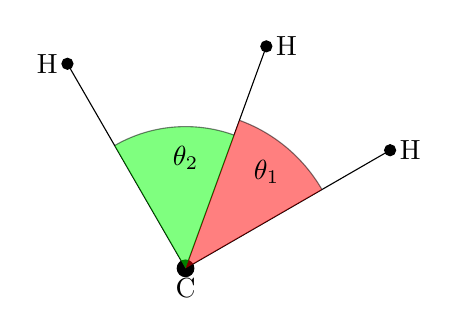
\begin{tikzpicture}

%\pgfmathsetmacro{\r}{3cm}
%\pgfmathsetmacro{\ho}{70}
%\pgfmathsetmacro{\ht}{30}
\newcommand{\radius}{3}
\newcommand{\hone}{120}
\newcommand{\htwo}{70}
\newcommand{\hthree}{30}

	\coordinate (O) at (0, 0);
	\coordinate (left) at ({\radius*cos(\hone)}, {\radius*sin(\hone)});
	\coordinate (right) at ({\radius*cos(\htwo)}, {\radius*sin(\htwo)});
	\coordinate (zero) at ({\radius*cos(\hthree)}, {\radius*sin(\hthree)});

	\draw[fill] (left) circle (2pt);
	\draw (left) node[below, left] {H};
	
	\draw[fill] (right) circle (2pt);
	\draw (right) node[right] {H};

	\draw[fill] (zero) circle (2pt);
	\draw (zero) node[right] {H};

	\draw[fill] (O) circle (3pt);
	\draw (O) node[below] {C};

	\draw (left) -- (O);
	\draw (right) -- (O);
	\draw (zero) -- (O);

	\begin{scope}
	\path[clip] (O) -- (right) -- (zero);
	\fill[red, opacity=0.5, draw=black] (O) circle (2);
	\node at ($(O)+(50:1.6)$) {$\theta_1$};	
	\end{scope}
	
	\begin{scope}
	\path[clip] (O) -- (left) -- (right);
	\fill[green, opacity=0.5, draw=black] (O) circle (1.8);
	\node at ($(O)+(90:1.4)$) {$\theta_2$};	
	\end{scope}	
  \end{tikzpicture}
\end{tabular}
\end{center}
\caption[The energy of a molecular configuration obeys the same symmetries as a M\"{o}bius strip]{An example of a function expressing the same symmetries as a M\"{o}bius strip in two of its arguments.  The energy of a molecular configuration $f(\theta_1, \theta_2)$ depends only on the relative angles between atoms, and because each atom is indistinguishable, is invariant to permuting the atoms. }
\label{fig:molecule}
\end{figure}

Figure \ref{fig:molecule} gives one example of a function which obeys the same symmetries as a M\"{o}bius strip, in some subsets of its arguments.

\fi

%
% A header that lets you compile a chapter by itself, or inside a larger document.
% Adapted from http://stackoverflow.com/questions/3655454/conditional-import-in-latex
%
%
%Use \inbpdocument and \outbpdocument in your individual files, in place of \begin{document} and \end{document}. In your main file, put in a \def \ismaindoc {} before including or importing anything.
%
% David Duvenaud
% June 2011
% 
% ======================================
%
%


\ifx\ismaindoc\undefined
	\newcommand{\inbpdocument}{
		\def \ismaindoc {}
		% Use this header if we are compiling by ourselves.
		\documentclass[a4paper,11pt,authoryear,index]{common/PhDThesisPSnPDF}
		
%\usepackage{draftwatermark}
%\SetWatermarkLightness{0.95}

% ******************************************************************************
% ****************************** Custom Margin *********************************

% Add `custommargin' in the document class options to use this section
% Set {innerside margin / outerside margin / topmargin / bottom margin}  and
% other page dimensions

\ifsetMargin
\else
    \RequirePackage[left=37mm,right=30mm,top=35mm,bottom=30mm]{geometry}
    \setFancyHdr % To apply fancy header after geometry package is loaded
\fi


%\chead{Unfinished draft}
%\cfoot{\texttt{Unfinished draft - compiled on \today{} at \currenttime}}

% *****************************************************************************
% ******************* Fonts (like different typewriter fonts etc.)*************

% Add `customfont' in the document class option to use this section

\ifsetFont
\else
    % Set your custom font here and use `customfont' in options. Leave empty to
    % load computer modern font (default LaTeX font).  

    \RequirePackage{libertine} 
\fi

% *****************************************************************************
% *************************** Bibliography  and References ********************

%\usepackage{cleveref} %Referencing without need to explicitly state fig /table

% Add `custombib' in the document class option to use this section
\ifsetBib % True, Bibliography option is chosen in class options
\else % If custom bibliography style chosen then load bibstyle here

   \RequirePackage[square, sort, numbers, authoryear]{natbib} % CustomBib

% If you would like to use biblatex for your reference management, as opposed to the default `natbibpackage` pass the option `custombib` in the document class. Comment out the previous line to make sure you don't load the natbib package. Uncomment the following lines and specify the location of references.bib file

% \RequirePackage[backend=biber, style=numeric-comp, citestyle=numeric, sorting=nty, natbib=true]{biblatex}
% \bibliography{References/references} %Location of references.bib only for biblatex

\fi


% changes the default name `Bibliography` -> `References'
\renewcommand{\bibname}{References}


% *****************************************************************************
% *************** Changing the Visual Style of Chapter Headings ***************
% Uncomment the section below. Requires titlesec package.

%\RequirePackage{titlesec}
%\newcommand{\PreContentTitleFormat}{\titleformat{\chapter}[display]{\scshape\Large}
%{\Large\filleft{\chaptertitlename} \Huge\thechapter}
%{1ex}{}
%[\vspace{1ex}\titlerule]}
%\newcommand{\ContentTitleFormat}{\titleformat{\chapter}[display]{\scshape\huge}
%{\Large\filleft{\chaptertitlename} \Huge\thechapter}{1ex}
%{\titlerule\vspace{1ex}\filright}
%[\vspace{1ex}\titlerule]}
%\newcommand{\PostContentTitleFormat}{\PreContentTitleFormat}
%\PreContentTitleFormat


% *****************************************************************************
% **************************** Custom Packages ********************************
% *****************************************************************************


% ************************* Algorithms and Pseudocode **************************

%\usepackage{algpseudocode} 


% ********************Captions and Hyperreferencing / URL **********************

% Captions: This makes captions of figures use a boldfaced small font. 
%\RequirePackage[small,bf]{caption}

\RequirePackage[labelsep=space,tableposition=top]{caption} 
%\renewcommand{\figurename}{Figure} %to support older versions of captions.sty
\captionsetup{belowskip=12pt,aboveskip=4pt}

% ************************ Formatting / Footnote *******************************

%\usepackage[perpage]{footmisc} %Range of footnote options 


% ****************************** Line Numbers **********************************

%\RequirePackage{lineno}
%\linenumbers

% ************************** Graphics and figures *****************************

%\usepackage{rotating}
%\usepackage{wrapfig}
%\usepackage{float}
\usepackage{subfig} %note: subfig must be included after the `caption` package. 


% ********************************* Table **************************************

%\usepackage{longtable}
%\usepackage{multicol}
%\usepackage{multirow}
%\usepackage{tabularx}


% ***************************** Math and SI Units ******************************

\usepackage{amsfonts}
\usepackage{amsmath}
\usepackage{amssymb}
%\usepackage{siunitx} % use this package module for SI units


% ******************************************************************************
% ************************* User Defined Commands ******************************
% ******************************************************************************

% *********** To change the name of Table of Contents / LOF and LOT ************

%\renewcommand{\contentsname}{My Table of Contents}
%\renewcommand{\listfigurename}{List of figures}
%\renewcommand{\listtablename}{List of tables}


% ********************** TOC depth and numbering depth *************************

\setcounter{secnumdepth}{2}
\setcounter{tocdepth}{2}

% ******************************* Nomenclature *********************************

% To change the name of the Nomenclature section, uncomment the following line

%\renewcommand{\nomname}{Symbols}


% ********************************* Appendix ***********************************

% The default value of both \appendixtocname and \appendixpagename is `Appendices'. These names can all be changed via: 

%\renewcommand{\appendixtocname}{List of appendices}
%\renewcommand{\appendixname}{Appndx}

		% All my custom preamble stuff.  Shouldn't overlap with anything in official-preamble


% Paths to figure and table directories.
\newcommand{\symmetryfigsdir}{figures/symmetries}
\newcommand{\topologyfiguresdir}{figures/topology}
\newcommand{\infinitefiguresdir}{figures/infinite}
\newcommand{\grammarfiguresdir}{figures/grammar}
\newcommand{\introfigsdir}{figures/intro}
\newcommand{\gplvmfiguresdir}{figures/gplvm}
\newcommand{\warpedfiguresdir}{figures/warped-mixtures}
\newcommand{\deeplimitsfiguresdir}{figures/deep-limits}
\newcommand{\quadraturefigsdir}{figures/quadrature}
\newcommand{\additivefigsdir}{figures/additive}
\newcommand{\decompfigsdir}{figures/decomp}
\newcommand{\examplefigsdir}{figures/worked-example}


\usepackage{bm}  % for warped mixtures - is this necessary?
\usepackage{booktabs}
\usepackage{tabularx}
\usepackage{multirow}
\usepackage{datetime}
\renewcommand{\tabularxcolumn}[1]{>{\arraybackslash}m{#1}}
\usepackage{relsize}
\usepackage{graphicx}
\usepackage{amsmath,amssymb,textcomp}
\usepackage{nicefrac}
\usepackage{amsthm}
\usepackage{tikz}
\usetikzlibrary{arrows}
\usetikzlibrary{calc}
\usepackage{nth}
\usepackage{rotating}
\usepackage{array}
\usepackage{fp}
\usepackage[hyperpageref]{backref}
\def\foo{\hspace{\fill}\mbox{}\linebreak[0]\hspace*{\fill}}
\renewcommand*{\backref}[1]{}
\renewcommand*{\backrefalt}[4]{%
\ifcase #1 %
%
\or
\foo(page #2)%
\else
\foo(pages #2)%
\fi
}

\usepackage{cleveref}
\crefname{equation}{equation}{equations}


%% For submission, make all render blank.
\input{common/commenting.tex}
%\renewcommand{\LATER}[1]{}
%\renewcommand{\fLATER}[1]{}
%\renewcommand{\TBD}[1]{}
%\renewcommand{\fTBD}[1]{}
%\renewcommand{\PROBLEM}[1]{}
%\renewcommand{\fPROBLEM}[1]{}
%\renewcommand{\NA}[1]{}


% HUMBLE WORDS: shown slightly smaller when in normal text
% Thanks to Christian Steinruecken!
\input{common/humble.tex}


% TODO: Clean up duplicates
\declareHumble{ANOVA}{ANOVA}
\declareHumble{ARD}{ARD}
\declareHumble{BIC}{BIC}
\declareHumble{BMC}{BMC}
\declareHumble{bq}{BQ}
\declareHumble{CRP}{CRP}
\declareHumble{dirpro}{DP}
\declareHumble{HDMR}{HDMR}
\declareHumble{GAM}{GAM}
\declareHumble{GEM}{GEM}
\declareHumble{GMM}{GMM}
\declareHumble{gplvm}{GP-LVM}
\declareHumble{gpml}{GPML}
\declareHumble{GPML}{GPML}
\declareHumble{gprn}{GPRN}
\declareHumble{gpt}{GP}
\declareHumble{gp}{GP}
\declareHumble{HKL}{HKL}
\declareHumble{HMC}{HMC}
\declareHumble{ibp}{IBP}
\declareHumble{iGMM}{iGMM}
\declareHumble{iwmm}{iWMM}
\declareHumble{kCP}{CP}
\declareHumble{kCW}{CW}
\declareHumble{kC}{C}
\declareHumble{KDE}{KDE}
\declareHumble{kLin}{Lin}
\declareHumble{KPCA}{KPCA}
\declareHumble{kPer}{Per}
\declareHumble{kRQ}{RQ}
\declareHumble{kSE}{SE}
\declareHumble{kWN}{WN}
\declareHumble{Lin}{Lin}
\declareHumble{LBFGS}{L-BFGS}
\declareHumble{mcmc}{MCMC}
\declareHumble{MKL}{MKL}
\declareHumble{MLP}{MLP}
\declareHumble{MSE}{MSE}
\declareHumble{Per}{Per}
\declareHumble{RMSE}{RMSE}
\declareHumble{RQ}{RQ}
\declareHumble{SBQ}{SBQ}
\declareHumble{seard}{SE-ARD}
\declareHumble{sefull}{SE-\textnormal{full}}
\declareHumble{SEGP}{SE-GP}
\declareHumble{SE}{SE}
\declareHumble{SNR}{SNR}
\declareHumble{SSANOVA}{SS-ANOVA}
\declareHumble{SVM}{SVM}

\newcommand{\kSig}{\boldsymbol\sigma}

\def\subexpr{{\cal S}}
\def\baseker{{\cal B}}
\def\numWinners{k}

\def\ie{i.e.\ }
\def\eg{e.g.\ }
\def\etc{etc.\ }
\let\oldemptyset\emptyset
\let\emptyset 0




% Unify notation between neural-net land and GP-land.
\newcommand{\hphi}{h}
\newcommand{\hPhi}{\vh}
\newcommand{\walpha}{w}
\newcommand{\wboldalpha}{\bw}
\newcommand{\wcapalpha}{\vW}
\newcommand{\lengthscale}{w}

\newcommand{\layerindex}{\ell}



\newcommand{\gpdrawbox}[1]{
\setlength\fboxsep{0pt}
\hspace{-0.15in} 
\fbox{
\includegraphics[width=0.464\columnwidth]{\deeplimitsfiguresdir/deep_draws/deep_gp_sample_layer_#1}
}}



\newcommand{\procedurename}{ABCD}
\newcommand{\genText}[1]{{\sf #1}}



\newcommand{\asdf}{$^{\textnormal{th}}$}

\newcommand{\binarysum}{\sum_{\bf{x} \in \{0,1\}^D}}
\newcommand{\expect}{\mathbb{E}}
\newcommand{\expectargs}[2]{\mathbb{E}_{#1} \left[ {#2} \right]}
\newcommand{\var}{\mathbb{V}}
\newcommand{\varianceargs}[2]{\mathbb{V}_{#1} \left[ {#2} \right]}
\newcommand{\cov}{\operatorname{cov}}
\newcommand{\Cov}{\operatorname{Cov}}
\newcommand{\covargs}[2]{\cov \left[ {#1}, {#2} \right]}
\newcommand{\variance}{\mathbb{V}}
\newcommand{\vecop}[1]{\operatorname{vec} \left( {#1} \right)}

\newcommand{\covarianceargs}[2]{\Cov_{#1} \left[ {#2} \right]}
\newcommand{\colvec}[2]{\left[ \begin{array}{c} {#1} \\ {#2} \end{array} \right]}
\newcommand{\tbtmat}[4]{\left[ \begin{array}{cc} {#1} & {#2} \\ {#3} & {#4} \end{array} \right]}

%\newcommand{\covskinny}[2]{\var\!\left(#1\middle\vert#2\right)} 

\newcommand{\acro}[1]{{\humble{#1}}}
%\newcommand{\vect}[1]{\boldsymbol{#1}}
\newcommand{\vect}[1]{{\bf{#1}}}
\newcommand{\mat}[1]{\mathbf{#1}}
\newcommand{\pderiv}[2]{\frac{\partial #1}{\partial #2}}
\newcommand{\npderiv}[2]{\nicefrac{\partial #1}{\partial #2}}

\newcommand{\pha}{^{\phantom{:}}}

\newcommand{\argmin}{\operatornamewithlimits{argmin}}
\newcommand{\argmax}{\operatornamewithlimits{argmax}}

% The following designed for probabilities with long arguments

\newcommand{\Prob}[2]{P\!\left(\,#1\;\middle\vert\;#2\,\right)}
\newcommand{\ProbF}[3]{P\!\left(\,#1\!=\!#2\;\middle\vert\;#3\,\right)}
\newcommand{\p}[2]{p\!\left(#1\middle\vert#2\right)}
\newcommand{\po}[1]{p\!\left(#1\right)}
\newcommand{\pF}[3]{p\!\left(\,#1\!=\!#2\;\middle\vert\;#3\,\right)} 
\newcommand{\mean}[2]{{m}\!\left(#1\middle\vert#2\right)}



\newcommand{\valpha}{\boldsymbol{\alpha}}
\newcommand{\va}{\vect{a}}
\newcommand{\vA}{\vect{A}}
\newcommand{\vB}{\mat{B}}
\newcommand{\vb}{\vect{b}}
\newcommand{\vC}{\mat{C}}
\newcommand{\vc}{\vect{c}}
\newcommand{\vecf}{\boldsymbol{f}}
\newcommand{\vell}{\vect{\ell}}
\newcommand{\vepsilon}{\boldsymbol{\epsilon}}
\newcommand{\veps}{\boldsymbol{\epsilon}}
\newcommand{\ve}{\boldsymbol{\epsilon}}
\newcommand{\vf}{\vecf}
\newcommand{\vg}{\vect{g}}
\newcommand{\vh}{\vect{h}}
\newcommand{\vI}{\mat{I}}
\newcommand{\vK}{\mat{K}}
\newcommand{\vk}{\vect{k}}
\newcommand{\vL}{\mat{L}}
\newcommand{\vl}{\vect{l}}
\newcommand{\vmu}{\boldsymbol{\mu}}
\newcommand{\vone}{\vect{1}}
\newcommand{\vphi}{\boldsymbol{\phi}}
\newcommand{\vpi}{\boldsymbol{\pi}}
\newcommand{\vq}{\vect{q}}
\newcommand{\vR}{\mat{R}}
\newcommand{\vr}{\vect{r}}
\newcommand{\vsigma}{\boldsymbol{\sigma}}
\newcommand{\vSigma}{\mat{\Sigma}}
\newcommand{\vS}{\mat{S}}
\newcommand{\vs}{\vect{s}}
\newcommand{\vtheta}{\boldsymbol{\theta}}
\newcommand{\vu}{\vect{u}}
\newcommand{\vV}{\mat{V}}
\newcommand{\vW}{\mat{W}}
\newcommand{\vw}{\vect{w}}
\newcommand{\vX}{\mat{X}}
\newcommand{\vx}{\vect{x}}
\newcommand{\vY}{\mat{Y}}
\newcommand{\vy}{\vect{y}}
\newcommand{\vzero}{\vect{0}}
\newcommand{\vZ}{\mat{Z}}
\newcommand{\vz}{\vect{z}}


\newcommand{\netweights}{\alpha}
\newcommand{\vnetweights}{\valpha}

\newcommand{\He}{\mathcal{H}}
\newcommand{\normx}[2]{\left\|#1\right\|_{#2}}
\newcommand{\Hnorm}[1]{\normx{#1}{\He}}
\newcommand{\mmd}{{\rm MMD}}


\newcommand{\mf}{\bar{\vf}}

%\newcommand{\mf}{\mu} %{\bar{\ell}}
\newcommand{\lf}{f} % Likelihood function
\newcommand{\st}{_\star}

% from simpler log-bq writeup
\newcommand{\lftwo}{{\log \ell}}
\newcommand{\mftwo}{{\bar \ell}}
\newcommand{\loggp}{{\log\acro{GP}}}%| \bX, \vy )}}
\newcommand{\loggpdist}{{\acro{GP}(\lftwo)}}%| \vX, \vy )}}


\newcommand{\inv}{^{{\mathsmaller{-1}}}}
\newcommand{\tohalf}{^{{\mathsmaller{\nicefrac{1}{2}}}}}

\newcommand{\Normal}{\mathcal{N}}
\newcommand{\N}[3]{\mathcal{N}\!\left(#1 \middle| #2,#3\right)}
\newcommand{\Nt}[2]{\mathcal{N}\!\left(#1,#2\right)}
\newcommand{\NT}[2]{\mathcal{N}\!\left(#1,#2\right)}
\newcommand{\GPdist}[3]{\mathcal{GP}\!\left(#1 \, \middle| \, #2, #3 \right)}
\newcommand{\bN}[3]{\mathcal{N}\big(#1 \middle| #2,#3\big)}
\newcommand{\boldN}[3]{\text{\textbf{\mathcal{N}}}\big(#1;#2,#3\big)}
\newcommand{\ones}[1]{\mat{1}_{#1}}
\newcommand{\eye}[1]{\mat{E}_{#1}}
\newcommand{\tra}{^{\mathsf{T}}}
%\newcommand{\tra}{^{\top}}
%\mathsf{T}
\newcommand{\trace}{\operatorname{tr}}
\newcommand{\shift}{\operatorname{shift}}
\renewcommand{\mod}{\operatorname{mod}}
\newcommand{\deq}{:=}
\newcommand{\oneofk}{\operatorname{one-of-k}}
%\newcommand{\degree}{^\circ}

\newcommand{\GPt}[2]{\mathcal{GP}\!\left(#1,#2\right)}
%\newcommand{\GPt}[2]{\gp\!\left(#1,#2\right)}

\DeclareMathOperator{\tr}{tr}
\DeclareMathOperator{\chol}{chol}
\DeclareMathOperator{\diag}{diag}

\newenvironment{narrow}[2]{%
  \begin{list}{}{%
  \setlength{\topsep}{0pt}%
  \setlength{\leftmargin}{#1}%
  \setlength{\rightmargin}{#2}%
  \setlength{\listparindent}{\parindent}%
  \setlength{\itemindent}{\parindent}%
  \setlength{\parsep}{\parskip}}%
\item[]}{\end{list}}



\newcommand{\dist}{\ \sim\ }
\def\given{\,|\,}

% Table stuff
\newcolumntype{C}[1]{>{\centering\let\newline\\\arraybackslash\hspace{0pt}}m{#1}}
\newcolumntype{L}[1]{>{\raggedright\let\newline\\\arraybackslash\hspace{0pt}}m{#1}}
\newcolumntype{R}[1]{>{\raggedleft\let\newline\\\arraybackslash\hspace{0pt}}m{#1}}


\def\ie{i.e.\ }
\def\eg{e.g.\ }
\def\iid{i.i.d.\ }
%\def\simiid{\sim_{\mbox{\tiny iid}}}
\def\simiid{\overset{\mbox{\tiny iid}}{\sim}}
\def\simind{\overset{\mbox{\tiny \textnormal{ind}}}{\sim}}
\def\eqdist{\stackrel{\mbox{\tiny d}}{=}}
%\newcommand{\distas}[1]{\mathbin{\overset{#1}{\kern \z@ \sim}}}
%TODO: fix this - it worked outside the thesis!
\newcommand{\distas}[1]{\mathbin{\overset{#1}{\sim}}}

\def\Reals{\mathbb{R}}

\def\Uniform{\mbox{\rm Uniform}}
\def\Bernoulli{\mbox{\rm Bernoulli}}
\def\GP{\mathcal{GP}}
\def\GPLVM{\mathcal{GP-LVM}}




% Kernel stuff

\def\iva{\vect{\inputVar}}
\def\ivaone{\inputVar}
\def\inputVar{x}
\def\InputVar{X}
\def\InputSpace{\mathcal{X}}
\def\outputVar{y}
\def\OutputSpace{\mathcal{Y}}
\def\function{f}
\def\kernel{k}
\def\KernelMatrix{K}
\def\SumKernel{\sum}
\def\ProductKernel{\prod}
\def\expression{e}
\def\feat{\vh}

\newcommand{\kerntimes}{ \! \times \!}
\newcommand{\kernplus}{ \, + \,}


% Proof stuff
\theoremstyle{plain}
\newtheorem{theorem}{Theorem}[section]
\newtheorem{lemma}[theorem]{Lemma}
\newtheorem{prop}[theorem]{Proposition}
\newtheorem{proposition}{Proposition}
\newtheorem*{cor}{Corollary}

% For infinite bq
\newcommand{\iv}{\theta}
\newcommand{\viv}{\vtheta}

% For intro chapter
\newcommand{\funcval}{\vf(\vX)}
\newcommand{\testpoint}{{\vx^\star}}

\newcommand{\underwrite}[2]{{\underbrace{#1}_{\textnormal{#2}}}}



% For kernel figures
\newcommand{\fhbig}{2cm}%
\newcommand{\fwbig}{3cm}%
\newcommand{\kernpic}[1]{\includegraphics[height=\fhbig,width=\fwbig]{\grammarfiguresdir/structure_examples/#1}}%
\newcommand{\kernpicr}[1]{\rotatebox{90}{\includegraphics[height=\fwbig,width=\fhbig]{\grammarfiguresdir/structure_examples/#1}}}%
\newcommand{\addkernpic}[1]{{\includegraphics[height=\fhbig,width=\fwbig]{\grammarfiguresdir/additive_multi_d/#1}}}%
\newcommand{\largeplus}{\tabbox{{\Large+}}}%
\newcommand{\largeeq}{\tabbox{{\Large=}}}%
\newcommand{\largetimes}{\tabbox{{\Large$\times$}}}%
\newcommand{\fixedx}{$x$ (with $x' = 1$)}%


		% ************************ Thesis Information & Meta-data **********************

%% The title of the thesis
%\title{Structured Gaussian Process Models} 
%\title{Automatic Model Construction \\ through \\ Structured Gaussian Processes}
%\title{Automatic Model-Building \\ through \\ Structured Gaussian Processes}
%\title{Automatic Modeling \\ with \\ Structured Gaussian Processes}    
\title{Automatic Model Construction \\ with Gaussian Processes}
%\title{Automatic Model Construction}
%\title{Automating Statistical Model Construction}


%\texorpdfstring is used for PDF metadata. Usage:
%\texorpdfstring{LaTeX_Version}{PDF Version (non-latex)} eg.,
%\texorpdfstring{$sigma$}{sigma}

%% The full name of the author
\author{David Kristjanson Duvenaud}

%% Department (eg. Department of Engineering, Maths, Physics)
%\dept{Department of Engineering}

%% University and Crest
\university{University of Cambridge}
\crest{\includegraphics[width=0.25\textwidth]{University_Crest}}

%% You can redefine the submission text:
% Default as per the University guidelines: This dissertation is submitted for
% the degree of Doctor of Philosophy
%\renewcommand{\submissiontext}{change the default text here if needed}

%% Full title of the Degree 
\degree{Doctor of Philosophy}
 
%% College affiliation (optional)
\college{Pembroke College}

%% Submission date
\degreedate{June 2014} 

%% Meta information
\subject{LaTeX} \keywords{{LaTeX} {PhD Thesis} {Engineering} {University of Cambridge}}



		\begin{document}
	}	
	\newcommand{\outbpdocument}[1]{

		% Fake chapters so references aren't broken
\label{ch:intro}                
\label{ch:kernels}
\label{ch:grammar}
\label{ch:description}
\label{ch:additive}
\label{ch:deeplimits}
\label{ch:discussion}
		%\bibliographystyle{common/CUEDthesis}
		\bibliographystyle{plainnat}
		\bibliography{references.bib}
		\end{document}
	}	
\else
	%If we're inside another document, no need to re-start the document.
	\ifx\inbpdocument\undefined
		\newcommand{\inbpdocument}{}
		\newcommand{\outbpdocument}[1]{}
	\fi
\fi

\inbpdocument


\chapter{Automatic Model Construction}
\label{ch:grammar}

\begin{quotation}
``It would be very nice to have a formal apparatus that gives us some `optimal' way of recognizing unusual phenomena and inventing new classes of hypotheses that are most likely to contain the true one; but this remains an art for the creative human mind.''
%``It would be very nice to have a formal apparatus that gives us some `optimal' way of recognizing unusual phenomena and inventing new classes of hypotheses \dots but this remains an art for the creative human mind.''
% In trying to practice this art, the Bayesian has the advantage because his formal apparatus already developed gives him a clearer picture of what to expect, and therefore a sharper perception for recognizing the unexpected.

\defcitealias{Jaynes85highlyinformative}{ -- E. T.  Jaynes (1985)}
\hspace*{\fill}\citetalias{Jaynes85highlyinformative}
\end{quotation}


In \cref{ch:kernels}, we saw that the choice of kernel determines the type of structure that can be learned by a \gp{} model, and that a wide variety of models could be constructed through simply adding and multiplying a few base kernels together.
However, we did not answer the difficult question of which kernel to use for a given problem.
Even for experts, choosing the kernel in \gp{} regression remains something of a black art.

The contribution of this chapter is to show how to automate the process of building kernels for \gp{} models.
To do so, we define an open-ended space of kernels, by adding and multiplying together kernels from a fixed set.
We then search over this space to find a kernel which captures as much structure in the data as possible.

Searching over such a large, structured model class has two main benefits.
First, this procedure has very good predictive accuracy, since it tries out a large number of different regression models.
Second, this procedure can discover interpretable structure in datasets.
Because \gp{} posteriors can be decomposed (as in \cref{sec:concrete}), we can also examine the resulting structures visually.
In \cref{ch:description}, we also show how to automatically generate English-language descriptions of the resulting models.

%\paragraph{Attribution}

This chapter is based on work done in collaboration with James Robert Lloyd, Roger Grosse, Joshua B. Tenenbaum, and Zoubin Ghahramani.
It was published in \citet{DuvLloGroetal13} and \citet{LloDuvGroetal14}.
Myself, James Lloyd and Roger Grosse jointly developed the idea of searching through a grammar-based language of \gp{} models, inspired by \citet{grosse2012exploiting}, and wrote the first versions of the code together.
James Lloyd ran most of the experiments, while I constructed most of the figures.
%I produced all of the figures.
%Zoubin Ghahramani and Josh Tenenbaum provided many conceptual insights, as well as suggestions about how the resulting procedure could be most fruitfully applied.

%\paragraph{Automatic statistician:} The work appearing in chapter \ref{ch:description} was written in collaboration with James Robert Lloyd, Roger Grosse, Joshua B. Tenenbaum, Zoubin Ghahramani, and was published in .
%The procedure translating kernels into adjectives grew out of discussions between James and myself.
%James Lloyd wrote the code to automatically generate reports, and ran all of the experiments.
%The text was written mainly by myself, James Lloyd, and Zoubin Ghahramani, with many helpful contributions and suggestions from Roger Grosse and Josh Tenenbaum.


%Section \ref{sec:Structure} outlines some commonly used kernel families as well as ways in which they can be composed. 
%Our grammar over kernels and our proposed structure discovery algorithm are described in Section \ref{sec:Search}. 
%Section \ref{sec:related_work} situates our work in the context of other nonparametric regression, kernel learning, and structure discovery methods.
%We evaluate our methods on synthetic datasets, time series analysis, and high-dimensional prediction problems in Sections \ref{sec:synthetic} through \ref{sec:quantitative}, respectively.




\section{Ingredients of an automatic statistician}
\label{sec:ingredients}
\citet{gelman2013philblogpost} asks, ``How can an artificial intelligence do statistics? ... It needs not just an inference engine, but also a way to construct new models and a way to check models. Currently, those steps are performed by humans, but the AI would have to do it itself.''.
%
This section will discuss the different parts we think are required to build an artificial intelligence that can do statistics.

\paragraph{1. An open-ended language of models.}
Many learning algorithms consider all models in a class of fixed size.
For example, graphical model learning algorithms \citep{Friedman03,Eaton07_uai} search over different connectivity graphs for a given set of nodes.
While such methods can be powerful, human statisticians are capable of deriving novel model classes when required.
An automatic search through an open-ended class of models can achieve some of this flexibility, growing the complexity of the model as needed, possibly combining existing structures in novel ways.

\paragraph{2. A search through model space.}
An open-ended space of models cannot be searched exhaustively.
Just as human researchers iteratively refine their models, search procedures can propose new search directions based on the results of previous model fits.
Because any search in an open-ended space must start with relatively simple models before moving on to more complex ones, any search strategy is likely to resemble an iterative model-building procedure.

\paragraph{3. A model comparison procedure.}
A search strategy requires an objective to optimize.
In this work, we use approximate marginal likelihood to compare models, penalizing complexity using the Bayesian Information Criterion as a heuristic.
More generally, an automatic statistician should be able to question the models it has constructed.
%, and formal procedures from model checking provide a way for it to do this.
\citet{gelman2012philosophy} review the literature on model checking.

\paragraph{4. A model description procedure.}
Part of the value of statistical models comes from helping humans to understand a dataset or a phenomenon.
Furthermore, a clear description of the statistical structure found in a dataset helps a user to notice when the dataset has errors, the wrong question was asked, the model-building procedure failed to capture known structure, a relevant piece of data or constraint is missing, or when a novel statistical structure has been found.

In this chapter, we introduce a system containing all the above ingredients.
We call this system the automatic Bayesian covariance discovery (\procedurename{}) system.
The next four sections of this chapter describe the mechanisms we use to produce these four ingredients, for this particular example of an artificial intelligence which does statistics.



\section{A language of regression models}
\label{sec:improvements}

As shown in \cref{ch:kernels}, we can construct a wide variety of kernel structures compositionally by adding and multiplying a small number of base kernels.
We can therefore define a language of \gp{} regression models simply by specifying a language of kernels.

\begin{figure}[ht!]%
\centering
\begin{tabular}{r|ccc}
Kernel name: & Rational quadratic (\kRQ) & Cosine ($\cos$) & White noise (\kLin) \\[10pt]
$k(x, x') =$ & $ \left( 1 + \frac{(\inputVar - \inputVar')^2}{2\alpha\ell^2}\right)^{-\alpha}$ &
$\cos\left(2 \pi \frac{ (x - x')}{p}\right)$ &
$\delta(\inputVar - \inputVar')$ \\[14pt]
\raisebox{1cm}{Plot of kernel:} & \kernpic{rq_kernel} & \kernpic{cos_kernel} & \kernpic{wn_kernel}\\
& $x -x'$ & $x -x'$ & \fixedx \\
%& & & \\
 & \large $\downarrow$ & \large $\downarrow$ & \large $\downarrow$  \\
\raisebox{1cm}{\parbox{2.5cm}{Samples from \gp{} prior:}} & \kernpic{rq_kernel_draws_s4} & \kernpic{cos_kernel_draws_s1} & \kernpic{wn_kernel_draws_s1} \\
Type of structure: & multiscale variation & sine waves & uncorrelated noise
\end{tabular}
\vspace{6pt}
\caption[Another set of basic kernels]
{New base kernels introduced in this chapter, and the types of structure they encode.
More interesting kernels can be constructed by adding and multiplying base kernels together.
%Left and third columns: base kernels $k(\cdot,0)$.
%Second and fourth columns: draws from a \sgp{} with each repective kernel.
%The x-axis has the same range on all plots.
}
\label{fig:basic_kernels_two}
\end{figure}
%
To specify an open-ended language of structured kernels, we will consider the set of all kernels that can be built by adding and multiplying these base kernels together:
\begin{align}
k_1 + k_2 =      & \,\, k_1(\vx, \vx') + k_2(\vx, \vx') \\
k_1 \times k_2 = & \,\, k_1(\vx, \vx') \times k_2(\vx, \vx')
%(k_1 + k_2)(\vx, \vx') =& \,\, k_1(\vx, \vx') + k_2(\vx, \vx')\\
%(k_1 \times k_2)(\vx, \vx') =& \,\, k_1(\vx, \vx') \times k_2(\vx, \vx')
\end{align}
%
This language of models is made out of a set of base kernels which capture different properties of functions, and a set of composition rules which combine kernels to yield other valid kernels.
In this chapter, we will use such base kernels as white noise ($\kWN$), constant ($\kC$), linear ($\kLin$), squared-exponential ($\kSE$), rational-quadratic ($\kRQ$), sigmoidal ($\kSig$) and periodic ($\kPer$).
We use a form of $\kPer$ due to James Lloyd (personal communication) which has its constant component removed, and $\cos(x - x')$ as a special case.
\Cref{fig:basic_kernels_two} shows the new kernels introduced in this chapter.
For precise definitions of all kernels, see appendix~\ref{sec:kernel-definitions}.

The space of kernels produced by adding and multiplying the above set of kernels contains many existing regression models.
\Cref{table:motifs} lists some of these, which are discussed in more detail in \cref{sec:gpss-related-work}. % regression models that can be expressed by this language.

\begin{table}[ht]
\centering
\begin{tabular}{l|l|l}
Regression model & Kernel & Related work\\
\midrule
Linear regression & $\kC \kernplus \kLin \kernplus \kWN$ & \\
Polynomial regression & $\kC \kernplus \prod \kLin \kernplus \kWN$ & \\
%Kernel ridge regression & $\kSE \kernplus \kWN$ & \\
Semi-parametric & $\kLin \kernplus \kSE \kernplus \kWN$ & \citet{ruppert2003semiparametric} \\
Multiple kernel learning & $\sum \kSE \kernplus \kWN$ & \citet{gonen2011multiple} \\
Trend, cyclical, irregular   & $\sum \kSE \kernplus \sum \kPer \kernplus \kWN$ & \citet{lind2006basic}\\
Fourier decomposition & $\kC \kernplus \sum \cos \kernplus \kWN$ & \\
Sparse spectrum \gp{}s & $\sum \cos \kernplus \kWN$ & \citet{lazaro2010sparse} \\
Spectral mixture & $\sum \SE \kerntimes \cos \kernplus \kWN$ & \citet{WilAda13} \\
Changepoints & \eg $\kCP(\kSE, \kSE) \kernplus \kWN$ & \citet{garnett2010sequential} \\
Time-changing variance & \eg $\kSE \kernplus \kLin \kerntimes \kWN$ & \\
Interpretable + flexible & $ \sum_d \kSE_d \kernplus \prod_d \kSE_d$ & \citet{plate1999accuracy} \\
Additive \gp{}s & $ \sum_{\vr \in \{0,1\}^D} \prod_{d \in \vr} \kSE_d$ & \cref{ch:additive}
\end{tabular}
\caption[Common regression models expressible in the kernel language]
{Common regression models expressible by sums and products of base kernels.
$\cos(\cdot, \cdot)$ is a special case of our reparametrised $\kPer(\cdot, \cdot)$.
}
\label{table:motifs}
\end{table}





\section{A model search procedure}

We explore the space of regression models using a simple greedy search.
At each stage, we choose the highest scoring kernel, and propose modifying it by applying an operation to one of its parts, combining or replacing that part with another base kernel.
The basic operations we can perform on any part $k$ of a kernel are:
%
\begin{center}
\begin{tabular}{rccc}
\textnormal{Replacement:}    & $\kernel$ & $\to$ & $\kernel'$\\
\textnormal{Addition:}       & $\kernel$ & $\to$ & $\kernel + \kernel'$\\
\textnormal{Multiplication:} & $\kernel$ &  $\to$ & $\kernel \times \kernel'$\\
\end{tabular}
\end{center}
%
where $k'$ is a new base kernel.
These operators can generate all possible algebraic expressions involving addition and multiplication of base kernels.
To see this, observe that if we restricted the addition and multiplication rules to only apply to base kernels, we would obtain a context-free grammar which generates the set of algebraic expressions.

\begin{figure}
\centering
%\begin{tabular}{cc}
%\begin{minipage}[t][14cm][t]{0.65\columnwidth}
\newcommand{\treescale}{*1.5\columnwidth}
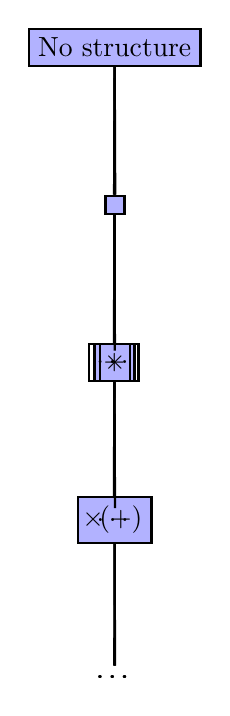
\begin{tikzpicture}
[sibling distance=0.15\treescale,-,thick, level distance=2cm]
%\footnotesize
\node[shape=rectangle,draw,thick,fill=blue!30] {No structure}
  child {node[shape=rectangle,draw,thick] {$\SE$}
  }
  child {node[shape=rectangle,draw,thick,fill=blue!30] {$\RQ$}
    [sibling distance=0.1\treescale]
    child {node[shape=rectangle,draw,thick] {$\SE$ + \RQ}}
    child {node {\ldots}}
    child {node[shape=rectangle,draw,thick,fill=blue!30] {$\Per + \RQ$}
      [sibling distance=0.15\treescale]
      child {node[shape=rectangle,draw,thick] {$\SE + \Per + \RQ$}}
      child {node {\ldots}}
      child {node[shape=rectangle,draw,thick,fill=blue!30] {$\SE \kerntimes (\Per + \RQ)$}
        [sibling distance=0.14\treescale]
        child {node {\ldots}}
        child {node {\ldots}}
        child {node {\ldots}}
      }
      child {node {\ldots}}
    }
    child {node {\ldots}}
    child {node[shape=rectangle,draw,thick] {$\Per \kerntimes \RQ$}}
  }
  child {node[shape=rectangle,draw,thick] {$\Lin$}
  }
  child {node[shape=rectangle,draw,thick] {$\Per$}
  };
\end{tikzpicture}
\caption[A search tree over kernels]{An example of a search tree over kernel expressions.
\Cref{fig:mauna_grow} shows the corresponding model increasing in sophistication as the kernel expression grows.
}
\label{fig:mauna_search_tree}
\end{figure}

\begin{figure}
\centering
\newcommand{\wmg}{0.31\columnwidth}  % width maunu growth
\newcommand{\hmg}{3.2cm}  % height maunu growth
\newcommand{\maunadecomp}[1]{\hspace{-0.15cm}
\includegraphics[width=\wmg,height=\hmg, clip,trim=0mm 0mm 0mm 7mm]{\grammarfiguresdir/decomposition/11-Feb-v4-03-mauna2003-s_max_level_#1/03-mauna2003-s_all_small}}
\begin{tabular}{ccc}
Level 1: & Level 2: & Level 3: \\
\RQ & $\Per + \RQ$ & $\SE \kerntimes (\Per + \RQ )$ \\[0.5em]
%Level 1: \RQ & Level 2: $\Per + \RQ$ & Level 3: $\SE \kerntimes (\Per + \RQ )$ \\[0.5em]
\maunadecomp{0} & \maunadecomp{1} & \maunadecomp{2} \\[0.5em]
\end{tabular}
\caption[Progression of models as the search depth increases]
{Posterior mean and variance for different depths of kernel search on the Mauna Loa dataset.
The dashed line marks the end of the dataset.
\emph{Left:} the function is only modeled as a locally smooth function, and the extrapolation is poor.
\emph{Middle:} a periodic component is added, and the extrapolation improves.
\emph{Right:} at depth 3, the kernel can capture most of the relevant structure, and is able to extrapolate reasonably.
}
\label{fig:mauna_grow}
\end{figure}

\Cref{fig:mauna_search_tree} shows an example search tree followed by our algorithm.
\Cref{fig:mauna_grow} shows how the resulting model changes as the search is followed.
In practice, we also include extra operators which propose commonly-occuring structures, such as changepoints.
A complete list is contained in appendix~\ref{sec:search-operators}.

Our search operators are motivated by strategies that human researchers often use to construct kernels.
In particular,
\begin{itemize}
\item One can look for structure, such as periodicity, in the residuals of a model, and then extend the model to capture that structure.
This corresponds to adding a new kernel to the existing structure.
\item One can start with structure, such as linearity, which is assumed to hold globally, but find that it only holds locally.
This corresponds to multiplying a kernel structure by a local kernel, such as $\kSE$.
\item One can add features incrementally, analogous to algorithms like boosting, back-fitting, or forward selection.
This corresponds to adding or multiplying with kernels on dimensions not yet included in the model.
\end{itemize}

%We stop the procedure at a fixed depth (typically 10), and return the best-scoring kernel over all depths.
%The fixed depth was enforcing solely for convencience - because the 




\subsubsection{Hyperparameter initialization}

Unfortunately, optimizing the marginal likelihood over parameters is not a convex optimization problem, and the space can have many local optima.
For example, in data with periodic structure, integer multiples of the true period (harmonics) are often local optima. 
We take advantage of our search procedure to provide reasonable initializations: all of the parameters which were part of the previous kernel are initialized to their previous values, while randomly initializing any newly introduced parameters.
In the newly proposed kernel, all parameters are then optimized using conjugate gradients.
This procedure is not guaranteed to find the global optimum, but it implements the commonly used heuristic of iteratively modeling residuals.






\section{A model comparison procedure}

Choosing a kernel requires a method for comparing models.
We choose marginal likelihood as our criterion, since it balances the fit and complexity of a model \citep{rasmussen2001occam}.
Conditioned on kernel parameters, the marginal likelihood of a \gp{} can be computed analytically.
Given a parametric form of a kernel, we can also choose its parameters using marginal likelihood.
However, choosing kernel parameters by maximum likelihood (as opposed to integrating them out) raises the possibility of overfitting.
In addition, if we compare two classes of kernels by the maximum likelihood found by optimizing over the kernel parameters, then all else being equal, the kernel class having more free parameters will be chosen.
This introduces a bias for more complex models.

We could avoid overfitting by integrating the marginal likelihood over all free parameters, but this integral is difficult to do in general.
Instead, we approximate this integral using the Bayesian information criterion (\BIC{}) \citep{schwarz1978estimating}:
%
\begin{equation}
\textrm{BIC}(M) = \log p(D \given M) - \frac{1}{2} |M| \log N
\end{equation}
%
where $p(D|M)$ is the marginal likelihood of the data (given by \cref{eq:gp_marg_lik}), $|M|$ is the number of kernel parameters, and $N$ is the number of data points.
\BIC{} simply penalizes the marginal likelihood in proportion to how many parameters the model has.
%BIC trades off model fit against model complexity and implements what is known as ``Bayesian Occam's Razor'' \citep{rasmussen2001occam,mackay2003information}.
Because BIC is a function of the number of parameters in a model, we did not count kernel parameters known to not affect the model.
For example, when two kernels are multiplied, one of their output variance parameters becomes redundant, and can be ignored.

Other more sophisticated approximations are possible, such as Laplace's approximation.
We chose to try \BIC{} first because of its simplicity, and it performed resonably in our experiments.




\section{A model description procedure}

As discussed in \Cref{ch:kernels}, a \gp{} whose kernel is a sum of kernels can be viewed as a sum of functions drawn from different \gp{}s.
We can always express any kernel structure as a sum of products of kernels, by distributing all products of sums.
For example,
%
\begin{align}
\SE \kerntimes (\RQ \kernplus \Lin) = \SE \kerntimes  \RQ \kernplus \SE \kerntimes \Lin
\end{align}
%
This decomposition into additive components provides a method of visualizing the learned model, breaking down the different types of structure discovered in the data.

For products of kernels which all apply to the same dimension, we can use the formulas in \cref{sec:posterior-variance} to visualize the marginal posterior distribution of each component.
The following section shows examples of such decomposition plots.
In \cref{ch:description}, we extend this model visualization method to include automatically generated English text explaining the meaning of each type of structure discovered.



\section{Structure discovery in time series}
\label{sec:time_series}

To investigate our method's ability to discover structure, we ran the kernel search on several time-series.
In the following examples, the search was run to depth 10, using \kSE{}, \kRQ{}, \kLin{}, \kPer{} and \kWN{} as base kernels.

\label{sec:extrapolation}
\subsection{Mauna Loa atmospheric CO$\mathbf{_{2}}$}

Using our method, we analyzed records of carbon dioxide levels recorded at the Mauna Loa observatory.
Since this dataset was analyzed in detail by \citet{rasmussen38gaussian}, we can compare the kernel chosen by our method to a kernel constructed by human experts.


\begin{figure}[ht!]
\newcommand{\wmgd}{0.5\columnwidth}  % width mauna decomp
\newcommand{\hmgd}{3.51cm}  % height mauna decomp
\newcommand{\mdrd}{\grammarfiguresdir/decomposition/11-Feb-03-mauna2003-s}  % mauna decomp results dir
\newcommand{\mbm}{\hspace{-0.2cm}}  % move back
\newcommand{\maunadgfx}[1]{\mbm \includegraphics[width=\wmgd,height=\hmgd, clip, trim=0mm 0mm 0mm 6mm]{\mdrd/03-mauna2003-s_#1}}
\begin{tabular}{cc}
\multicolumn{2}{c}{
\begin{tabular}{c}
Complete model: 
$\kLin \kerntimes \kSE + \kSE \kerntimes ( \kPer + \RQ ) \kernplus \kWN$ \\
\maunadgfx{all}
\end{tabular}
} \\\\
%\multicolumn{2}{c}{Decomposition} \\
Long-term trend: $\Lin \kerntimes \SE$ & Yearly periodic: $\SE \kerntimes \Per$ \\
\maunadgfx{1} & \maunadgfx{2_zoom} \\[1em]
Medium-term deviation: $\SE \kerntimes \RQ$ & Noise: \kWN \\
\maunadgfx{3} & \maunadgfx{resid}
\end{tabular}
\caption[Decomposition of the Mauna Loa model]
{\emph{First row:} The full posterior on the Mauna Loa dataset, after a search of depth 10.
\emph{Subsequent rows:} The automatic decomposition of the time series.
The model is a sum of long-term, yearly periodic, medium-term components, and residual noise, respectively.
The yearly periodic component has been rescaled for clarity.}
\label{fig:mauna_decomp}
\end{figure}



\Cref{fig:mauna_grow} shows the posterior mean and variance on this dataset as the search depth increases.
While the data can be smoothly interpolated by a model with only a single base kernel, the extrapolations improve dramatically as the increased search depth allows more structure to be included.

\Cref{fig:mauna_decomp} shows the final model chosen by our method, together with its decomposition into additive components.
The final model exhibits both plausible extrapolation and interpretable components: a long-term trend, annual periodicity, and medium-term deviations.
These are the same components chosen in the kernel hand-constructed by \citet[Chapter 5]{rasmussen38gaussian}.

We also plot the residuals modeled by a white noise ($\kWN$) component, showing that there is little obvious structure left in the data.
More generally, some components capture slowly-changing structure while others capture quickly-varying struture, but there is no hard distinction between ``signal'' components and ``noise'' components.





\subsection{Airline passenger counts}

\begin{figure}[h!]
\centering
\newcommand{\wagd}{0.48\columnwidth}  % width airline decomp
\newcommand{\hagd}{4cm}  % height airline decomp
\newcommand{\mb}{\hspace{-0.2cm}}  % move back
%\newcommand{\ard}{../figures/decomposition/11-Feb-01-airline-s}  % airline results dir
%\newcommand{\ard}{\grammarfiguresdir/decomposition/31-Jan-v301-airline-months}  % airline results dir
%
% Level 5 of 
% https://github.com/jamesrobertlloyd/gpss-research/blob/master/results/2014-01-14-GPSS-add/01-airline_result.txt
%SumKernel(SqExp, Product[NoiseKernel LinearKernel], ProductKernel[SqExp, PeriodicKernel, LinearKernel, ProductKernel[SqExpKernel, LinearKernel])])
\newcommand{\ard}{\grammarfiguresdir/decomposition/19-Jan-2014-airline-months}  % airline results dir
\newcommand{\airdgfx}[1]{\mb \includegraphics[width=\wagd,height=\hagd, clip, trim=10mm 0mm 14mm 8mm]{\ard/#1} }
%
\begin{tabular}{cc}
\multicolumn{2}{c}{
\begin{tabular}{c}
Complete Model: $\kSE \kerntimes \Lin \kernplus \kPer \kerntimes \kLin \kerntimes \kSE \kernplus \kSE \kernplus \kWN \kerntimes \kLin$ \\
\airdgfx{01-airline_all}
\end{tabular}
} \\
Long-term trend: $\kSE \kerntimes \Lin$ & Yearly periodic: $\kPer \kerntimes \Lin \kerntimes \kSE$ \\
\airdgfx{01-airline_1_extrap} & \airdgfx{01-airline_2_extrap} \\
Medium-term deviation: $\kSE$ & Growing noise: $\kWN \kerntimes \Lin$ \\
\airdgfx{01-airline_3_extrap} & \airdgfx{01-airline_4_extrap}
\end{tabular}
\caption[Decomposition of airline dataset model]
{\emph{First row:} The airline dataset and posterior after a search of depth 10.
\emph{Subsequent rows:} Additive decomposition of posterior into long-term smooth trend, yearly variation, and short-term deviations.
Due to the linear kernel, the marginal variance grows over time, making this a heteroskedastic model. 
}
\label{fig:airline_decomp}
\end{figure}

\Cref{fig:airline_decomp} shows the decomposition produced by applying our method to monthly totals of international airline passengers~\citep{box2013time}.
We observe similar components to those in the Mauna Loa dataset: a long term trend, annual periodicity, and medium-term deviations.
In addition, the composite kernel captures the near-linearity of the long-term trend, and the linearly growing amplitude of the annual oscillations.

% Created by the command:
% postprocessing.make_all_1d_figures(folder='../results/31-Jan-1d/', prefix='31-Jan-v3', rescale=False)





\section{Related work}
\label{sec:gpss-related-work}

\def\rwsheader{\subsubsection}

\rwsheader{Building kernel functions by hand}
\citet[chapter 5]{rasmussen38gaussian} devoted 4 pages to manually constructing a composite kernel to model the Mauna Loa dataset.
%In the supplementary material, we include a report automatically generated by \procedurename{} for this dataset; our procedure chose a model similar to the one they constructed by hand.
Other examples of papers whose main contribution is to manually construct and fit a composite \gp{} kernel are \citet{textperiodic13}, \citet{lloydgefcom2012}, and \citet{EdgarTelescope}.


\rwsheader{Nonparametric regression in high dimensions}
Nonparametric regression methods such as splines, locally-weighted regression, and \gp{} regression are popular because they are capable of learning arbitrary smooth functions of the data.
Unfortunately, they suffer from the curse of dimensionality: it is very difficult for these models to generalize well in more than a few dimensions.

Applying nonparametric methods in high-dimensional spaces can require imposing additional structure on the model.
One such structure is additivity.
Generalized additive models~\citep{hastie1990generalized} assume the regression function is a transformed sum of functions defined on the individual dimensions: $\expect[f(\vx)] = g\inv(\sum_{d=1}^D f_d(x_d))$.
These models have a limited compositional form, but one which is interpretable and often generalizes well.
In our grammar, we can capture such structure through sums of base kernels along different dimensions, although we have not yet tried incorporating a warping function $g(\cdot)$.

It is possible to add more flexibility to additive models by considering higher-order interactions between different dimensions. 
\Cref{ch:additive} considers \gp{} models whose kernel implicitly sums over all possible interactions of input variables.
\citet{plate1999accuracy} constructs a special case of this model class, summing an \kSE{} kernel along each dimension, plus a single \seard{} kernel (a product of \kSE{} over all dimensions).
Both of these models can be expressed in our grammar.

A closely related procedure is smoothing-splines \ANOVA{} \citep{wahba1990spline, gu2002smoothing}.
This model is a linear combinations of splines along each dimension, all pairs of dimensions, and possibly higher-order combinations.
Because the number of terms to consider grows exponentially in the order, in practice, only terms of first and second order are usually considered.

Semi-parametric regression \citep[e.g.][]{ruppert2003semiparametric} attempts to combine interpretability with flexibility by building a composite model out of an interpretable, parametric part (such as linear regression) and a `catch-all' nonparametric part (such as a \gp{} with an \kSE{} kernel).
This model class can be represented through the kernel ${\kSE \kernplus \kLin}$.


\rwsheader{Kernel learning}
There is a large body of work attempting to construct a rich kernel through a weighted sum of many base kernels \citep[e.g.][]{gonen2011multiple, Bach_HKL}.
These approaches usually admit a convex objective function.
However the component kernels, as well as their parameters, must be specified in advance.

%Another approach to kernel learning is to learn an embedding of the data points. 
%\citet{lawrence2005probabilistic} learns an embedding of the data into a low-dimensional space, using a fixed kernel structure over that space.
%This model is typically used in unsupervised tasks and requires an expensive integration or optimisation over potential embeddings when generalizing to test points.

\citet{salakhutdinov2008using} use a deep neural network with unsupervised pre-training to learn an embedding $g(\vx)$ onto which a \gp{} with an $\kSE$ kernel is placed: ${\Cov{[f(\vx), f(\vx')]} = k(g(\vx), g(\vx'))}$.
This is a flexible approach to kernel learning, but relies upon finding structure in the input density $p(\vx)$.
Instead, we focus on domains where most of the interesting structure is in $f(\vx)$.

Sparse spectrum \gp{}s \citep{lazaro2010sparse} approximate the spectral density of a stationary kernel function using delta functions which corresponds to kernels of the form $\sum \cos$.
Similarly, \citet{WilAda13} introduce spectral mixture kernels, which approximate the spectral density using a mixture of Gaussians -- corresponding to kernels of the form $\sum \kSE \times \cos$.
Both groups demonstrate, using Bochner's theorem \citep{bochner1959lectures}, that these kernels can approximate any stationary covariance function.
Our language of kernels includes both of these kernel classes (see \cref{table:motifs}).

There is a large body of work attempting to construct rich kernels through a weighted sum of base kernels called multiple kernel learning (\MKL{}) \citep[e.g.][]{bach2004multiple}.
These approaches find the optimal solution in polynomial time, but only if the component kernels and parameters are pre-specified.
We compare to a Bayesian variant of \MKL{} in \cref{sec:numerical}, expressed as a restriction of our language of kernels.


\rwsheader{Equation learning}
\cite{todorovski1997declarative}, \cite{washio1999discovering} and \cite{Schmidt2009b} learn parametric forms of functions specifying time series, or relations between quantities.
In contrast, \procedurename{} learns a parametric form for the covariance, allowing it to model functions which do not have a simple parametric form but still have high-level structure.
An examination of the structure discovered by the automatic equation-learning software Eureqa \citep{Eureqa} on the airline and Mauna Loa datasets can be found in \citet{LloDuvGroetal14}.
%\Cref{sec:eqn-learning-comp}.



\rwsheader{Structure discovery through grammars}


\citet{kemp2008discovery} learned the structural form of a graph used to model human similarity judgements.
Their grammar on graph structures includes planes, trees, and cylinders.
Some of their discrete graph structures have continuous analogues in our own space.
For example, $\SE_1 \kerntimes \SE_2$ and $\SE_1 \kerntimes \Per_2$ can be seen as mapping the data to a plane and a cylinder, respectively.
\Cref{sec:topological-manifolds} examines these structures in more detail.

\citet{diosan2007evolving} and \citet{bing2010gp} learn composite kernels for support vector machines and relevance vector machines, respectively, using genetic search algorithms to optimize cross-validation error.
Similarly, \citet{kronberger2013evolution} search over composite kernels for \gp{}s using genetic programming, optimizing the unpenalized marginal likelihood.
These methods explore similar languages of kernels to the one explored in this chapter.
%However, each of these methods suffer either from a model selection criterion which is not differentiable with respect to kernel parameters (cross-validation of classification accuracy), or from one which does not penalize complexity of the resulting kernel expressions.
It is not clear whether the complex genetic searches used by these methods offer advantages over the straightforward but na\"{i}ve greedy search used in this chapter.
%However, \citet{kronberger2013evolution} observed overfitting
%Our work goes beyond ths prior work by demonstrating the structure implied by composite kernels, employing a Bayesian search criterion, and allowing for the automatic discovery of interpretable structure from data.
Our search criterion has the advantages of being both differentiable with respect to kernel parameters, and trading off model fit and complexity automatically.
This prior work also did not explore the automatic model decomposition, summarization and description made possible by the use of \gp{} models.
% and goes beyond this prior work by demonstrating the interpretability of the structure implied by composite kernels, and how such structure allows for extrapolation.


\citet{grosse2012exploiting} performed a greedy search over a compositional model class for unsupervised learning, using a grammar of matrix decomposition models, and a greedy search procedure based on held-out likelihood.
This model class contains many existing unsupervised models as special cases, and was able to discover such structure automatically from data.
Our framework takes a similar approach, but in a supervised setting.

Similarly, \citet{christian-thesis} showed to automatically perform inference in arbitrary compositions of discrete sequence models.
More generally, \citet{dechter2013bootstrap} and \citet{liang2010learning} constructed grammars over programs, and automatically searched the resulting spaces.




\section{Experiments}
\label{sec:numerical}

\subsection{Interpretability versus accuracy}

BIC trades off model fit and complexity by penalizing the number of parameters in a kernel expression.
This can result in \procedurename{} favoring kernel expressions with nested products of sums, producing descriptions involving many additive components when expressions are expanded.
While these models typically have good predictive performance, the large number of components can make them less interpretable.
We experimented with not allowing parentheses during the search, discouraging nested expressions.
This was achieved by distributing all products immediately after each search operator was applied.
We call this procedure \procedurename{}-interpretability, in contrast to the unrestricted version of the search, \procedurename{}-accuracy.


\subsection{Predictive accuracy on time series}


%\subsubsection{Datasets}

We evaluate the performance of the algorithms listed below on 13 real time-series from various domains from the time series data library \citep{TSDL}.
% plots of the data can be found at the beginning of the reports in the supplementary material.



\subsubsection{Algorithms}

We compare \procedurename{} to equation learning using Eureqa \citep{Eureqa}, as well as six other regression algorithms:
linear regression,
\gp{} regression with a single $\kSE$ kernel (squared exponential),
a Bayesian variant of multiple kernel learning (\MKL{}) \citep[e.g.][]{gonen2011multiple, bach2004multiple},
changepoint modeling \citep[e.g.][]{garnett2010sequential, saatcci2010gaussian, FoxDunson:NIPS2012},
spectral mixture kernels \citep{WilAda13} (spectral kernels),
and trend-cyclical-irregular models \citep[e.g.][]{lind2006basic}.

We set Eureqa's search objective to the default mean-absolute-error.
All algorithms besides Eureqa can be expressed as restrictions of our modeling language (see \cref{table:motifs}), so we perform inference using the same search and objective function, with appropriate restrictions to the language.
For \MKL{}, trend-cyclical-irregular, and spectral kernels, the greedy search procedure of \procedurename{} corresponds to a forward-selection algorithm.
For squared-exponential and linear regression, the procedure corresponds to standard marginal likelihood optimization.
%More advanced inference methods are sometimes used for changepoint modeling, but we use the same inference method for all algorithms for comparability.

We restricted to regression algorithms for comparability; we did not include models which regress on previous values of times series, such as auto-regressive or moving-average models \citep[e.g.][]{box2013time}.
Constructing a language of autoregressive time-series models would be an interesting area for future research.



\subsubsection{Extrapolation experiments}

To test extrapolation, we trained all algorithms on the first 90\% of the data, predicted the remaining 10\% and then computed the root mean squared error (\RMSE{}).
The \RMSE{}s are then standardised by dividing by the smallest \RMSE{} for each data set, so the best performance on each data set will have a value of 1.

\begin{figure}[h!]
\includegraphics[width=1.02\textwidth]{\grammarfiguresdir/comparison/box_extrap_wide}
\caption[Extrapolation error of all methods on 13 time-series datasets]
{Box plot (showing median and quartiles) of standardised extrapolation \RMSE{} (best performance = 1) on 13 time-series.
The methods are ordered by median.
}
\label{fig:box_extrap_dist}
\end{figure}


\Cref{fig:box_extrap_dist} shows the standardised \RMSE{}s across algorithms.
\procedurename{}-accuracy outperforms \procedurename{}-interpretability.
Both algorithms have lower quartiles than all other methods.

Overall, the model construction methods with greater capacity perform better: \procedurename{} outperforms trend-cyclical-irregular, which outperforms Bayesian \MKL{}, which outperforms squared-exponential.
Despite searching over a rich model class, Eureqa performs relatively poorly, since very few datasets are parsimoniously explained by a parametric equation.

Not shown on the plot are large outliers for spectral kernels, Eureqa, squared exponential and linear regression with normalized \RMSE{}s of 11, 493, 22 and 29 respectively.
%All of these outliers occurred on a data set with a large discontinuity (see the call centre data in the supplementary material).

%\subsubsection{Interpolation}
%To test the ability of the methods to interpolate, we randomly divided each data set into equal amounts of training data and testing data.
%The results are similar to those for extrapolation, and are included in \cref{sec:interpolation-appendix}.

%\fTBD{Josh: Can you write about the Blessing of abstraction, and doing lots with a small amount of data?  This might become apparent from plotting the extraplolations.}
%\fTBD{RBG: We could make this point as part of the learning curves for extrapolation by marking the points at which each additional aspect of the structure is found.}





\subsection{High-dimensional prediction}

\procedurename{} can also be applied to multidimensional regression problems without modification.
An experimental comparison with other methods can be found in \cref{sec:additive-experiments}, where it outperforms a wide variety of multidimensional regression methods.



\subsection{Structure recovery on synthetic data}
\label{sec:synthetic}

The structure found in the examples above may seem reasonable, but we may wonder to what extent \procedurename{} is consistent - that is, when do we recover all the structure in any given dataset?
It is difficult to tell from predictive accuracy alone if the search procedure is finding the correct structure, especially in multiple dimensions.
To address this question, we tested our method's ability to recover known structure on a set of synthetic datasets.

For several composite kernel expressions, we constructed synthetic data by first sampling 300 points uniformly at random, then sampling function values at those points from a \gp{} prior.
We then added \iid Gaussian noise to the functions at various signal-to-noise ratios (\SNR{}).


\begin{table}[ht!]
\caption[Kernels recovered on synthetic data]
{
Kernels chosen by our method on synthetic data generated using known kernel structures. $D$ denotes the dimension of the functions being modeled.
\SNR{} indicates the signal-to-noise ratio.
Dashes (--) indicate no structure was found.
Each kernel implicitly has a \kWN{} kernel included.
}
\label{tbl:synthetic}
\addtolength{\tabcolsep}{1pt}
\setlength\extrarowheight{2pt}
\begin{center}
{\small
\begin{tabular}{c c | c c c}
True kernel & $D$ & \SNR{} = 10 & \SNR{} = 1 & \hspace{-1cm} \SNR{} = 0.1 \\
\hline
$\SE \kernplus \RQ$        & 1 & $\SE$ & $\SE \kerntimes \Per$ & $\SE$ \\
$\Lin \kerntimes \Per$ & 1 & $\Lin \kerntimes \Per$ & $\Lin \kerntimes \Per$ & $\SE$ \\
$\SE_1 \kernplus \RQ_2$    & 2 & $\SE_1 \kernplus \SE_2$ & $\Lin_1 \kernplus \SE_2$ & $\Lin_1$ \\
$\SE_1 \kernplus \SE_2 \kerntimes \Per_1 \kernplus \SE_3$ & 3 & $\SE_1 \kernplus \SE_2 \kerntimes \Per_1 \kernplus \SE_3$ & $\SE_2 \kerntimes \Per_1 \kernplus \SE_3$ & -- \\
$\SE_1 \kerntimes \SE_2$ & 4 & $\SE_1 \kerntimes \SE_2$ & $\Lin_1 \kerntimes \SE_2$ & $\Lin_2$ \\
$\SE_1 \kerntimes \SE_2 \kernplus \SE_2 \kerntimes \SE_3$ & 4 & $\SE_1 \kerntimes \SE_2 \kernplus \SE_2 \kerntimes \SE_3$ & $\SE_1 \kernplus \SE_2 \kerntimes \SE_3$ & $\SE_1$ \\
\multirow{2}{*}{ $(\SE_1 \kernplus \SE_2) \kerntimes (\SE_3 \kernplus \SE_4)$ } & \multirow{2}{*}{4} & $(\SE_1 \kernplus \SE_2) \, \kerntimes$ \dots & $(\SE_1 \kernplus \SE_2) \, \kerntimes$ \dots & \multirow{2}{*}{--} \\
 & & $(\SE_3\kerntimes\Lin_3\kerntimes\Lin_1 \kernplus \SE_4)$ & $\SE_3 \kerntimes \SE_4$ &
\end{tabular}
}
\end{center}
\end{table}


\Cref{tbl:synthetic} shows the results.
For the highest \SNR{}, the method finds all relevant structure except in one case.
The reported additional linear structure in the last row is explainable by the fact that functions sampled from \kSE{} kernels with long length-scales occasionally have near-linear trends.
As the noise increases, our method generally backs off to simpler structures, rather than over-fitting.

\subsubsection{Source code}
Source code to perform all experiments is available at \url{github.com/jamesrobertlloyd/gpss-research}. 
All \gp{} parameter optimisation was performed by automated calls to the \GPML{} toolbox, available at \url{gaussianprocess.org/gpml/code}.


\section{Discussion}

This chapter presented a system which constructs an appropriate model from an open-ended language, and automatically generates plots decomposing the different types of structure present in the model.

This was done by introducing a space of kernels defined by sums and products of a small number of base kernels.  
The set of models in this space includes many standard regression models.
We proposed a search procedure for this space of kernels, and argued that this search process parallels the process of model-building by statisticians.

We found that the learned structures are often capable of accurate extrapolation in time-series datasets, and are competitive with widely used kernel classes and kernel combination methods on a variety of prediction tasks.
The learned kernels often yield decompositions of a signal into diverse and interpretable components, enabling model-checking by humans.
We hope that this procedure has the potential to make powerful statistical model-building techniques accessible to non-experts.

The next chapter will show how the model components found by this procedure can be automatically described using English-language text.

\iffalse
\section{Future Work}

\subsubsection{Structure search in classification}
While we focus on Gaussian process regression, the kernel search method could be applied to other supervised learning problems such as classification or ordinal regression.
%, or to other kinds of kernel architectures such as kernel \SVM{}s.
However, it might be more difficult to discover structure from class labels alone, since they usually contain less information about the underlying process than regression targets.
%However, whether or not such modularity and interpretability is present in other model classes is an open question.

\subsubsection{Improving the search}
The search procedure used in this chapter leaves much room for improvement.
Presumably, some sort of model-based search would be worthwhile, since evaluating each kernel expression is relatively expensive.
This raises the question of how to build an open-ended model of the relative marginal likelihood of \gp{} models.
In order to use a \gp{} for this task, one would need to create a kernel over kernels, as in \citet{ong2002hyperkernels}.

One interesting possibility is that the model of model performance could generate its own data offline.
The system could generate synthetic regression datasets, then score many kernel structures on those datasets in order to improve its model of kernel performance.

%\subsubsection{Building languages of other model classes}
%The compositionality of diverse types of kernels is what allowed a rich language of \gp{} models.
%Can we build similar languages of other model classes?

%As noted in \cref{sec:gpss-related-work}, languages have already been constructed on several powerful model classes: matrix decompositions, sequence models, graphical models, and functional programs.
%Building languages of models that support efficient search as well as interpretable decompositions could be a fruitful direction.
%\citet{roger-grosse-thesis} demonstrated a very rich class of unsupervised models by composing matrix decompositions.
%\citet{kemp2008discovery} and \citet{ellislearning} built grammars on graphical models.

\subsubsection{Use in model-based optimization}
The automatic model-building procedure described in this chapter could also be used in the inner loop of \gp{}-based Bayesian optimization routines, such as \citet{snoek2012practical}.
Discovering structure such as additivity in a problem could be expected to decrease the number of samples needed.


\subsubsection{Incroporating uncertainty in the structure}
\fi


\outbpdocument{
\bibliographystyle{plainnat}
\bibliography{references.bib}
}

%
% A header that lets you compile a chapter by itself, or inside a larger document.
% Adapted from http://stackoverflow.com/questions/3655454/conditional-import-in-latex
%
%
%Use \inbpdocument and \outbpdocument in your individual files, in place of \begin{document} and \end{document}. In your main file, put in a \def \ismaindoc {} before including or importing anything.
%
% David Duvenaud
% June 2011
% 
% ======================================
%
%


\ifx\ismaindoc\undefined
	\newcommand{\inbpdocument}{
		\def \ismaindoc {}
		% Use this header if we are compiling by ourselves.
		\documentclass[a4paper,11pt,authoryear,index]{common/PhDThesisPSnPDF}
		
%\usepackage{draftwatermark}
%\SetWatermarkLightness{0.95}

% ******************************************************************************
% ****************************** Custom Margin *********************************

% Add `custommargin' in the document class options to use this section
% Set {innerside margin / outerside margin / topmargin / bottom margin}  and
% other page dimensions

\ifsetMargin
\else
    \RequirePackage[left=37mm,right=30mm,top=35mm,bottom=30mm]{geometry}
    \setFancyHdr % To apply fancy header after geometry package is loaded
\fi


%\chead{Unfinished draft}
%\cfoot{\texttt{Unfinished draft - compiled on \today{} at \currenttime}}

% *****************************************************************************
% ******************* Fonts (like different typewriter fonts etc.)*************

% Add `customfont' in the document class option to use this section

\ifsetFont
\else
    % Set your custom font here and use `customfont' in options. Leave empty to
    % load computer modern font (default LaTeX font).  

    \RequirePackage{libertine} 
\fi

% *****************************************************************************
% *************************** Bibliography  and References ********************

%\usepackage{cleveref} %Referencing without need to explicitly state fig /table

% Add `custombib' in the document class option to use this section
\ifsetBib % True, Bibliography option is chosen in class options
\else % If custom bibliography style chosen then load bibstyle here

   \RequirePackage[square, sort, numbers, authoryear]{natbib} % CustomBib

% If you would like to use biblatex for your reference management, as opposed to the default `natbibpackage` pass the option `custombib` in the document class. Comment out the previous line to make sure you don't load the natbib package. Uncomment the following lines and specify the location of references.bib file

% \RequirePackage[backend=biber, style=numeric-comp, citestyle=numeric, sorting=nty, natbib=true]{biblatex}
% \bibliography{References/references} %Location of references.bib only for biblatex

\fi


% changes the default name `Bibliography` -> `References'
\renewcommand{\bibname}{References}


% *****************************************************************************
% *************** Changing the Visual Style of Chapter Headings ***************
% Uncomment the section below. Requires titlesec package.

%\RequirePackage{titlesec}
%\newcommand{\PreContentTitleFormat}{\titleformat{\chapter}[display]{\scshape\Large}
%{\Large\filleft{\chaptertitlename} \Huge\thechapter}
%{1ex}{}
%[\vspace{1ex}\titlerule]}
%\newcommand{\ContentTitleFormat}{\titleformat{\chapter}[display]{\scshape\huge}
%{\Large\filleft{\chaptertitlename} \Huge\thechapter}{1ex}
%{\titlerule\vspace{1ex}\filright}
%[\vspace{1ex}\titlerule]}
%\newcommand{\PostContentTitleFormat}{\PreContentTitleFormat}
%\PreContentTitleFormat


% *****************************************************************************
% **************************** Custom Packages ********************************
% *****************************************************************************


% ************************* Algorithms and Pseudocode **************************

%\usepackage{algpseudocode} 


% ********************Captions and Hyperreferencing / URL **********************

% Captions: This makes captions of figures use a boldfaced small font. 
%\RequirePackage[small,bf]{caption}

\RequirePackage[labelsep=space,tableposition=top]{caption} 
%\renewcommand{\figurename}{Figure} %to support older versions of captions.sty
\captionsetup{belowskip=12pt,aboveskip=4pt}

% ************************ Formatting / Footnote *******************************

%\usepackage[perpage]{footmisc} %Range of footnote options 


% ****************************** Line Numbers **********************************

%\RequirePackage{lineno}
%\linenumbers

% ************************** Graphics and figures *****************************

%\usepackage{rotating}
%\usepackage{wrapfig}
%\usepackage{float}
\usepackage{subfig} %note: subfig must be included after the `caption` package. 


% ********************************* Table **************************************

%\usepackage{longtable}
%\usepackage{multicol}
%\usepackage{multirow}
%\usepackage{tabularx}


% ***************************** Math and SI Units ******************************

\usepackage{amsfonts}
\usepackage{amsmath}
\usepackage{amssymb}
%\usepackage{siunitx} % use this package module for SI units


% ******************************************************************************
% ************************* User Defined Commands ******************************
% ******************************************************************************

% *********** To change the name of Table of Contents / LOF and LOT ************

%\renewcommand{\contentsname}{My Table of Contents}
%\renewcommand{\listfigurename}{List of figures}
%\renewcommand{\listtablename}{List of tables}


% ********************** TOC depth and numbering depth *************************

\setcounter{secnumdepth}{2}
\setcounter{tocdepth}{2}

% ******************************* Nomenclature *********************************

% To change the name of the Nomenclature section, uncomment the following line

%\renewcommand{\nomname}{Symbols}


% ********************************* Appendix ***********************************

% The default value of both \appendixtocname and \appendixpagename is `Appendices'. These names can all be changed via: 

%\renewcommand{\appendixtocname}{List of appendices}
%\renewcommand{\appendixname}{Appndx}

		% All my custom preamble stuff.  Shouldn't overlap with anything in official-preamble


% Paths to figure and table directories.
\newcommand{\symmetryfigsdir}{figures/symmetries}
\newcommand{\topologyfiguresdir}{figures/topology}
\newcommand{\infinitefiguresdir}{figures/infinite}
\newcommand{\grammarfiguresdir}{figures/grammar}
\newcommand{\introfigsdir}{figures/intro}
\newcommand{\gplvmfiguresdir}{figures/gplvm}
\newcommand{\warpedfiguresdir}{figures/warped-mixtures}
\newcommand{\deeplimitsfiguresdir}{figures/deep-limits}
\newcommand{\quadraturefigsdir}{figures/quadrature}
\newcommand{\additivefigsdir}{figures/additive}
\newcommand{\decompfigsdir}{figures/decomp}
\newcommand{\examplefigsdir}{figures/worked-example}


\usepackage{bm}  % for warped mixtures - is this necessary?
\usepackage{booktabs}
\usepackage{tabularx}
\usepackage{multirow}
\usepackage{datetime}
\renewcommand{\tabularxcolumn}[1]{>{\arraybackslash}m{#1}}
\usepackage{relsize}
\usepackage{graphicx}
\usepackage{amsmath,amssymb,textcomp}
\usepackage{nicefrac}
\usepackage{amsthm}
\usepackage{tikz}
\usetikzlibrary{arrows}
\usetikzlibrary{calc}
\usepackage{nth}
\usepackage{rotating}
\usepackage{array}
\usepackage{fp}
\usepackage[hyperpageref]{backref}
\def\foo{\hspace{\fill}\mbox{}\linebreak[0]\hspace*{\fill}}
\renewcommand*{\backref}[1]{}
\renewcommand*{\backrefalt}[4]{%
\ifcase #1 %
%
\or
\foo(page #2)%
\else
\foo(pages #2)%
\fi
}

\usepackage{cleveref}
\crefname{equation}{equation}{equations}


%% For submission, make all render blank.
\input{common/commenting.tex}
%\renewcommand{\LATER}[1]{}
%\renewcommand{\fLATER}[1]{}
%\renewcommand{\TBD}[1]{}
%\renewcommand{\fTBD}[1]{}
%\renewcommand{\PROBLEM}[1]{}
%\renewcommand{\fPROBLEM}[1]{}
%\renewcommand{\NA}[1]{}


% HUMBLE WORDS: shown slightly smaller when in normal text
% Thanks to Christian Steinruecken!
\input{common/humble.tex}


% TODO: Clean up duplicates
\declareHumble{ANOVA}{ANOVA}
\declareHumble{ARD}{ARD}
\declareHumble{BIC}{BIC}
\declareHumble{BMC}{BMC}
\declareHumble{bq}{BQ}
\declareHumble{CRP}{CRP}
\declareHumble{dirpro}{DP}
\declareHumble{HDMR}{HDMR}
\declareHumble{GAM}{GAM}
\declareHumble{GEM}{GEM}
\declareHumble{GMM}{GMM}
\declareHumble{gplvm}{GP-LVM}
\declareHumble{gpml}{GPML}
\declareHumble{GPML}{GPML}
\declareHumble{gprn}{GPRN}
\declareHumble{gpt}{GP}
\declareHumble{gp}{GP}
\declareHumble{HKL}{HKL}
\declareHumble{HMC}{HMC}
\declareHumble{ibp}{IBP}
\declareHumble{iGMM}{iGMM}
\declareHumble{iwmm}{iWMM}
\declareHumble{kCP}{CP}
\declareHumble{kCW}{CW}
\declareHumble{kC}{C}
\declareHumble{KDE}{KDE}
\declareHumble{kLin}{Lin}
\declareHumble{KPCA}{KPCA}
\declareHumble{kPer}{Per}
\declareHumble{kRQ}{RQ}
\declareHumble{kSE}{SE}
\declareHumble{kWN}{WN}
\declareHumble{Lin}{Lin}
\declareHumble{LBFGS}{L-BFGS}
\declareHumble{mcmc}{MCMC}
\declareHumble{MKL}{MKL}
\declareHumble{MLP}{MLP}
\declareHumble{MSE}{MSE}
\declareHumble{Per}{Per}
\declareHumble{RMSE}{RMSE}
\declareHumble{RQ}{RQ}
\declareHumble{SBQ}{SBQ}
\declareHumble{seard}{SE-ARD}
\declareHumble{sefull}{SE-\textnormal{full}}
\declareHumble{SEGP}{SE-GP}
\declareHumble{SE}{SE}
\declareHumble{SNR}{SNR}
\declareHumble{SSANOVA}{SS-ANOVA}
\declareHumble{SVM}{SVM}

\newcommand{\kSig}{\boldsymbol\sigma}

\def\subexpr{{\cal S}}
\def\baseker{{\cal B}}
\def\numWinners{k}

\def\ie{i.e.\ }
\def\eg{e.g.\ }
\def\etc{etc.\ }
\let\oldemptyset\emptyset
\let\emptyset 0




% Unify notation between neural-net land and GP-land.
\newcommand{\hphi}{h}
\newcommand{\hPhi}{\vh}
\newcommand{\walpha}{w}
\newcommand{\wboldalpha}{\bw}
\newcommand{\wcapalpha}{\vW}
\newcommand{\lengthscale}{w}

\newcommand{\layerindex}{\ell}



\newcommand{\gpdrawbox}[1]{
\setlength\fboxsep{0pt}
\hspace{-0.15in} 
\fbox{
\includegraphics[width=0.464\columnwidth]{\deeplimitsfiguresdir/deep_draws/deep_gp_sample_layer_#1}
}}



\newcommand{\procedurename}{ABCD}
\newcommand{\genText}[1]{{\sf #1}}



\newcommand{\asdf}{$^{\textnormal{th}}$}

\newcommand{\binarysum}{\sum_{\bf{x} \in \{0,1\}^D}}
\newcommand{\expect}{\mathbb{E}}
\newcommand{\expectargs}[2]{\mathbb{E}_{#1} \left[ {#2} \right]}
\newcommand{\var}{\mathbb{V}}
\newcommand{\varianceargs}[2]{\mathbb{V}_{#1} \left[ {#2} \right]}
\newcommand{\cov}{\operatorname{cov}}
\newcommand{\Cov}{\operatorname{Cov}}
\newcommand{\covargs}[2]{\cov \left[ {#1}, {#2} \right]}
\newcommand{\variance}{\mathbb{V}}
\newcommand{\vecop}[1]{\operatorname{vec} \left( {#1} \right)}

\newcommand{\covarianceargs}[2]{\Cov_{#1} \left[ {#2} \right]}
\newcommand{\colvec}[2]{\left[ \begin{array}{c} {#1} \\ {#2} \end{array} \right]}
\newcommand{\tbtmat}[4]{\left[ \begin{array}{cc} {#1} & {#2} \\ {#3} & {#4} \end{array} \right]}

%\newcommand{\covskinny}[2]{\var\!\left(#1\middle\vert#2\right)} 

\newcommand{\acro}[1]{{\humble{#1}}}
%\newcommand{\vect}[1]{\boldsymbol{#1}}
\newcommand{\vect}[1]{{\bf{#1}}}
\newcommand{\mat}[1]{\mathbf{#1}}
\newcommand{\pderiv}[2]{\frac{\partial #1}{\partial #2}}
\newcommand{\npderiv}[2]{\nicefrac{\partial #1}{\partial #2}}

\newcommand{\pha}{^{\phantom{:}}}

\newcommand{\argmin}{\operatornamewithlimits{argmin}}
\newcommand{\argmax}{\operatornamewithlimits{argmax}}

% The following designed for probabilities with long arguments

\newcommand{\Prob}[2]{P\!\left(\,#1\;\middle\vert\;#2\,\right)}
\newcommand{\ProbF}[3]{P\!\left(\,#1\!=\!#2\;\middle\vert\;#3\,\right)}
\newcommand{\p}[2]{p\!\left(#1\middle\vert#2\right)}
\newcommand{\po}[1]{p\!\left(#1\right)}
\newcommand{\pF}[3]{p\!\left(\,#1\!=\!#2\;\middle\vert\;#3\,\right)} 
\newcommand{\mean}[2]{{m}\!\left(#1\middle\vert#2\right)}



\newcommand{\valpha}{\boldsymbol{\alpha}}
\newcommand{\va}{\vect{a}}
\newcommand{\vA}{\vect{A}}
\newcommand{\vB}{\mat{B}}
\newcommand{\vb}{\vect{b}}
\newcommand{\vC}{\mat{C}}
\newcommand{\vc}{\vect{c}}
\newcommand{\vecf}{\boldsymbol{f}}
\newcommand{\vell}{\vect{\ell}}
\newcommand{\vepsilon}{\boldsymbol{\epsilon}}
\newcommand{\veps}{\boldsymbol{\epsilon}}
\newcommand{\ve}{\boldsymbol{\epsilon}}
\newcommand{\vf}{\vecf}
\newcommand{\vg}{\vect{g}}
\newcommand{\vh}{\vect{h}}
\newcommand{\vI}{\mat{I}}
\newcommand{\vK}{\mat{K}}
\newcommand{\vk}{\vect{k}}
\newcommand{\vL}{\mat{L}}
\newcommand{\vl}{\vect{l}}
\newcommand{\vmu}{\boldsymbol{\mu}}
\newcommand{\vone}{\vect{1}}
\newcommand{\vphi}{\boldsymbol{\phi}}
\newcommand{\vpi}{\boldsymbol{\pi}}
\newcommand{\vq}{\vect{q}}
\newcommand{\vR}{\mat{R}}
\newcommand{\vr}{\vect{r}}
\newcommand{\vsigma}{\boldsymbol{\sigma}}
\newcommand{\vSigma}{\mat{\Sigma}}
\newcommand{\vS}{\mat{S}}
\newcommand{\vs}{\vect{s}}
\newcommand{\vtheta}{\boldsymbol{\theta}}
\newcommand{\vu}{\vect{u}}
\newcommand{\vV}{\mat{V}}
\newcommand{\vW}{\mat{W}}
\newcommand{\vw}{\vect{w}}
\newcommand{\vX}{\mat{X}}
\newcommand{\vx}{\vect{x}}
\newcommand{\vY}{\mat{Y}}
\newcommand{\vy}{\vect{y}}
\newcommand{\vzero}{\vect{0}}
\newcommand{\vZ}{\mat{Z}}
\newcommand{\vz}{\vect{z}}


\newcommand{\netweights}{\alpha}
\newcommand{\vnetweights}{\valpha}

\newcommand{\He}{\mathcal{H}}
\newcommand{\normx}[2]{\left\|#1\right\|_{#2}}
\newcommand{\Hnorm}[1]{\normx{#1}{\He}}
\newcommand{\mmd}{{\rm MMD}}


\newcommand{\mf}{\bar{\vf}}

%\newcommand{\mf}{\mu} %{\bar{\ell}}
\newcommand{\lf}{f} % Likelihood function
\newcommand{\st}{_\star}

% from simpler log-bq writeup
\newcommand{\lftwo}{{\log \ell}}
\newcommand{\mftwo}{{\bar \ell}}
\newcommand{\loggp}{{\log\acro{GP}}}%| \bX, \vy )}}
\newcommand{\loggpdist}{{\acro{GP}(\lftwo)}}%| \vX, \vy )}}


\newcommand{\inv}{^{{\mathsmaller{-1}}}}
\newcommand{\tohalf}{^{{\mathsmaller{\nicefrac{1}{2}}}}}

\newcommand{\Normal}{\mathcal{N}}
\newcommand{\N}[3]{\mathcal{N}\!\left(#1 \middle| #2,#3\right)}
\newcommand{\Nt}[2]{\mathcal{N}\!\left(#1,#2\right)}
\newcommand{\NT}[2]{\mathcal{N}\!\left(#1,#2\right)}
\newcommand{\GPdist}[3]{\mathcal{GP}\!\left(#1 \, \middle| \, #2, #3 \right)}
\newcommand{\bN}[3]{\mathcal{N}\big(#1 \middle| #2,#3\big)}
\newcommand{\boldN}[3]{\text{\textbf{\mathcal{N}}}\big(#1;#2,#3\big)}
\newcommand{\ones}[1]{\mat{1}_{#1}}
\newcommand{\eye}[1]{\mat{E}_{#1}}
\newcommand{\tra}{^{\mathsf{T}}}
%\newcommand{\tra}{^{\top}}
%\mathsf{T}
\newcommand{\trace}{\operatorname{tr}}
\newcommand{\shift}{\operatorname{shift}}
\renewcommand{\mod}{\operatorname{mod}}
\newcommand{\deq}{:=}
\newcommand{\oneofk}{\operatorname{one-of-k}}
%\newcommand{\degree}{^\circ}

\newcommand{\GPt}[2]{\mathcal{GP}\!\left(#1,#2\right)}
%\newcommand{\GPt}[2]{\gp\!\left(#1,#2\right)}

\DeclareMathOperator{\tr}{tr}
\DeclareMathOperator{\chol}{chol}
\DeclareMathOperator{\diag}{diag}

\newenvironment{narrow}[2]{%
  \begin{list}{}{%
  \setlength{\topsep}{0pt}%
  \setlength{\leftmargin}{#1}%
  \setlength{\rightmargin}{#2}%
  \setlength{\listparindent}{\parindent}%
  \setlength{\itemindent}{\parindent}%
  \setlength{\parsep}{\parskip}}%
\item[]}{\end{list}}



\newcommand{\dist}{\ \sim\ }
\def\given{\,|\,}

% Table stuff
\newcolumntype{C}[1]{>{\centering\let\newline\\\arraybackslash\hspace{0pt}}m{#1}}
\newcolumntype{L}[1]{>{\raggedright\let\newline\\\arraybackslash\hspace{0pt}}m{#1}}
\newcolumntype{R}[1]{>{\raggedleft\let\newline\\\arraybackslash\hspace{0pt}}m{#1}}


\def\ie{i.e.\ }
\def\eg{e.g.\ }
\def\iid{i.i.d.\ }
%\def\simiid{\sim_{\mbox{\tiny iid}}}
\def\simiid{\overset{\mbox{\tiny iid}}{\sim}}
\def\simind{\overset{\mbox{\tiny \textnormal{ind}}}{\sim}}
\def\eqdist{\stackrel{\mbox{\tiny d}}{=}}
%\newcommand{\distas}[1]{\mathbin{\overset{#1}{\kern \z@ \sim}}}
%TODO: fix this - it worked outside the thesis!
\newcommand{\distas}[1]{\mathbin{\overset{#1}{\sim}}}

\def\Reals{\mathbb{R}}

\def\Uniform{\mbox{\rm Uniform}}
\def\Bernoulli{\mbox{\rm Bernoulli}}
\def\GP{\mathcal{GP}}
\def\GPLVM{\mathcal{GP-LVM}}




% Kernel stuff

\def\iva{\vect{\inputVar}}
\def\ivaone{\inputVar}
\def\inputVar{x}
\def\InputVar{X}
\def\InputSpace{\mathcal{X}}
\def\outputVar{y}
\def\OutputSpace{\mathcal{Y}}
\def\function{f}
\def\kernel{k}
\def\KernelMatrix{K}
\def\SumKernel{\sum}
\def\ProductKernel{\prod}
\def\expression{e}
\def\feat{\vh}

\newcommand{\kerntimes}{ \! \times \!}
\newcommand{\kernplus}{ \, + \,}


% Proof stuff
\theoremstyle{plain}
\newtheorem{theorem}{Theorem}[section]
\newtheorem{lemma}[theorem]{Lemma}
\newtheorem{prop}[theorem]{Proposition}
\newtheorem{proposition}{Proposition}
\newtheorem*{cor}{Corollary}

% For infinite bq
\newcommand{\iv}{\theta}
\newcommand{\viv}{\vtheta}

% For intro chapter
\newcommand{\funcval}{\vf(\vX)}
\newcommand{\testpoint}{{\vx^\star}}

\newcommand{\underwrite}[2]{{\underbrace{#1}_{\textnormal{#2}}}}



% For kernel figures
\newcommand{\fhbig}{2cm}%
\newcommand{\fwbig}{3cm}%
\newcommand{\kernpic}[1]{\includegraphics[height=\fhbig,width=\fwbig]{\grammarfiguresdir/structure_examples/#1}}%
\newcommand{\kernpicr}[1]{\rotatebox{90}{\includegraphics[height=\fwbig,width=\fhbig]{\grammarfiguresdir/structure_examples/#1}}}%
\newcommand{\addkernpic}[1]{{\includegraphics[height=\fhbig,width=\fwbig]{\grammarfiguresdir/additive_multi_d/#1}}}%
\newcommand{\largeplus}{\tabbox{{\Large+}}}%
\newcommand{\largeeq}{\tabbox{{\Large=}}}%
\newcommand{\largetimes}{\tabbox{{\Large$\times$}}}%
\newcommand{\fixedx}{$x$ (with $x' = 1$)}%


		% ************************ Thesis Information & Meta-data **********************

%% The title of the thesis
%\title{Structured Gaussian Process Models} 
%\title{Automatic Model Construction \\ through \\ Structured Gaussian Processes}
%\title{Automatic Model-Building \\ through \\ Structured Gaussian Processes}
%\title{Automatic Modeling \\ with \\ Structured Gaussian Processes}    
\title{Automatic Model Construction \\ with Gaussian Processes}
%\title{Automatic Model Construction}
%\title{Automating Statistical Model Construction}


%\texorpdfstring is used for PDF metadata. Usage:
%\texorpdfstring{LaTeX_Version}{PDF Version (non-latex)} eg.,
%\texorpdfstring{$sigma$}{sigma}

%% The full name of the author
\author{David Kristjanson Duvenaud}

%% Department (eg. Department of Engineering, Maths, Physics)
%\dept{Department of Engineering}

%% University and Crest
\university{University of Cambridge}
\crest{\includegraphics[width=0.25\textwidth]{University_Crest}}

%% You can redefine the submission text:
% Default as per the University guidelines: This dissertation is submitted for
% the degree of Doctor of Philosophy
%\renewcommand{\submissiontext}{change the default text here if needed}

%% Full title of the Degree 
\degree{Doctor of Philosophy}
 
%% College affiliation (optional)
\college{Pembroke College}

%% Submission date
\degreedate{June 2014} 

%% Meta information
\subject{LaTeX} \keywords{{LaTeX} {PhD Thesis} {Engineering} {University of Cambridge}}



		\begin{document}
	}	
	\newcommand{\outbpdocument}[1]{

		% Fake chapters so references aren't broken
\label{ch:intro}                
\label{ch:kernels}
\label{ch:grammar}
\label{ch:description}
\label{ch:additive}
\label{ch:deeplimits}
\label{ch:discussion}
		%\bibliographystyle{common/CUEDthesis}
		\bibliographystyle{plainnat}
		\bibliography{references.bib}
		\end{document}
	}	
\else
	%If we're inside another document, no need to re-start the document.
	\ifx\inbpdocument\undefined
		\newcommand{\inbpdocument}{}
		\newcommand{\outbpdocument}[1]{}
	\fi
\fi

\inbpdocument


\chapter{Automatic Model Description}
\label{ch:description}

\begin{quotation}
``When I write, I feel like an armless, legless man with a crayon in his mouth.''

\hspace*{\fill} \emph{ -- Kurt Vonnegut}
\end{quotation}




%The compositional structure of the language described in the previous chapter 
The previous chapter showed how to automatically build structured models through a language of kernels.
It also showed how to decompose the resulting models into the different types of structure present, and how to visually illustrate the type of structure captured by each component.
This chapter will show how automatically describe the resulting model structures with English text.

The model decomposition plots of \cref{ch:grammar}, show that most of the structure present in each component was determined by that component's kernel.
Even across different datasets, the meaning of the individual parts of those kernels is relatively consistent.
For example, $\kPer$ usually indicates some sort of repeating structure, and $\kSE$ usually indicates smooth change over time.
This chapter shows how to take advantage of this modularity to develop a method for automatically describing the structure represented by components of structured \gp{} models through text.
The main idea is to treat every component of a product kernel as an adjective, or as a short phrase which modifies the description of a kernel.

% descriptions of patterns in the data.
%In this chapter, we describe how \procedurename{} can generate natural-language descriptions of the models found by the search procedure.
Combining model search, plots, and text, we present a system which automatically generates reports which highlight interpretable features discovered in a variety of data sets.
An example of a complete automatically-generated report can be found in \cref{ch:example-solar}.
%Other example reports can be found at \url{mlg.eng.cam.ac.uk/Lloyd/abcdoutput/}
% (e.g.\ figure~\ref{fig:periodic}).

The work appearing in this chapter was written in collaboration with James Robert Lloyd, Roger Grosse, Joshua B. Tenenbaum, Zoubin Ghahramani, and was published in \citep{LloDuvGroetal14}.
The procedure translating kernels into adjectives grew out of discussions between James and myself.
James Lloyd wrote the code to automatically generate reports, and ran all of the experiments.
%The text was written mainly by myself, James Lloyd, and Zoubin Ghahramani, with many helpful contributions and suggestions from Roger Grosse and Josh Tenenbaum.


\section{Generating Descriptions of Kernels}

There are two main features of our language of \gp{} models that allow description to be performed automatically.
First, the sometimes complicated kernel expressions found by the model search can always be simplified into a sum of products.
As discussed in \cref{ch:kernels}, a sum of kernels corresponds to a sum of functions, so each product can be described separately.
Second, each kernel in a product modifies the resulting model in a consistent way.
Therefore, to generate a description of a product of kernels, we can describe one kernel using a noun with all others described using adjectives.

For example, we can describe the product of kernels $\kPer \kerntimes \kSE$ by representing $\kPer$ by a noun (``a periodic function'') modified by a phrase representing the effect of the $\kSE$ kernel (``whose shape varies smoothly over time'').
To simplify the system, we restrict the base kernels to $\kC$, $\kLin$, $\kWN$, $\kSE$, $\kPer$, and $\vsigma$ (allowing changepoints and change-windows).


\subsection{Simplification Rules}

In order to be able to use the same adjectives to for each type of kernel in different circumstances, we must convert each kernel expression into a standard, simplified form.

We do this by first distributing all products of sums into a sum of products.
Then, we apply several simplifications to the kernel expression:

\begin{itemize}
\item Products of two or more $\kSE$ kernels can be equivalently represented by a single $\kSE$ with different parameters.
\item Multiplying the white-noise kernel $\kWN$ by any stationary kernel ($\kC$, $\kWN$, $\kSE$, or $\kPer$) gives another $\kWN$ kernel.
\item Multiplying any kernel by $\kC$ only changes the parameters of the original kernel, and so can be factored out of any product in which it appears.
\end{itemize}

After applying these rules, any kernel can be written as a sum of terms of the form:
\begin{align}
K \prod_m \kLin^{(m)} \prod_n \boldsymbol\sigma^{(n)},
\label{eq:sop}
\end{align}
where $K$ is one of $\{\kWN, \kC, \kSE, \prod_k \kPer^{(k)}\}$ or $\{\kSE \prod_k \kPer^{(k)}\}$, 
where $\prod_i\kernel^{(i)}$ denotes a product of kernels, each with different parameters.
We use superscripts to distinguish between different instances of the same kernel appearing in a product: $\SE^{(1)}$ can have different kernel parameters than $\kSE^{(2)}$.


%\subsubsection{Sums of kernels are sums of functions}
%Formally, if $f_1(x) \dist \gp{}(0, \kernel_1)$ and independently $f_2(x) \dist \gp{}(0, \kernel_2)$ then ${f_1(x) + f_2(x) \dist \gp{}(0, \kernel_1 + \kernel_2)}$.
%Because sums of kernels correspond to sums of functions, we can describe each product of kernels separately.

\subsection{Describing Each Kernel in a Product}

Loosely speaking, each kernel in a product modifies the resulting \gp{} model in a consistent way.
This allows us to describe the contribution of each kernel in a product as an adjective, or more generally as a post-modifier of a noun.
We now describe how each of the kernels in our grammar modifies a \gp{} model.
%, and how this effect can be described in natural language:

\begin{itemize}
\item {\bf Multiplication by $\kSE$} removes long range correlations from a model since, $\kSE(x,x')$ decreases monotonically to 0 as $|x - x'|$ increases.
%This can be described as making an existing model's correlation structure `local' or `approximate'.
This will convert any global correlation structure into local correlation only.

\item {\bf Multiplication by $\kLin$} is equivalent to multiplying the function being modeled by a linear function.
If $f(x) \dist \gp{}(0, \kernel)$, then $xf(x) \dist \gp{}\left(0, \kLin \kerntimes k \right)$.
This causes the standard deviation of the model to vary linearly without affecting the correlation.
% and can be described as \eg `with linearly increasing standard deviation'.

\item {\bf Multiplication by $\boldsymbol\sigma$} is equivalent to multiplying the function being modeled by a sigmoid, which means that the function goes to zero before or after some point.
%This can be described as \eg `from [time]' or `until [time]'.

\item {\bf Multiplication by $\kPer$}
modifies the correlation structure in the same way as multiplying the function by an independent periodic function.
This follows from the fact that if ${f_1(x) \dist \gp{}(0, \kernel_1)}$ and ${f_2(x) \dist \gp{}(0, \kernel_2)}$ then
\begin{align}
{\textrm{Cov} \left[f_1(x)f_2(x), f_1(x')f_2(x') \right] = k_1(x,x')k_2(x,x')}.
\end{align}
%This can be loosely described as \eg `modulated by a periodic function with a period of [period] [units]'.
Put more plainly, a \gp{} whose covariance is a product of kernels has the same covariance (but not necessarily the same higher moments) as a product of two functions, each drawn from the corresponding \gp{} prior.
This identity holds for any two kernels, and can be used to generate a cumbersome ``worst-case'' description in cases where a more meaningful description of the effect of a kernel is not obvious.
\end{itemize}

\begin{table}[h!]
\centering
\begin{tabular}{l|l}
Kernel & Postmodifier phrase \\
\midrule
$\kSE$  & whose shape changes smoothly \\
$\kPer$ & modulated by a periodic function \\
$\kLin$ & with linearly varying amplitude \\
$\prod_k \kLin^{(k)}$ & with polynomially varying amplitude \\
$\prod_k \boldsymbol{\sigma}^{(k)}$ & which applies until / from [changepoint] \\
\end{tabular}
\caption[Descriptions of the effect of each kernel, written as a post-modifier]{
Descriptions of the effect of each kernel, written as a post-modifier.
}
\label{table:modifiers}
\end{table}

\Cref{table:modifiers} gives the corresponding description of the effect of adding each type of kernel to a product, written as a post-modifier.
%
\begin{table}[h!]
\centering
\begin{tabular}{l|l}
Kernel & Noun phrase \\
\midrule
$\kWN$  & uncorrelated noise \\
$\kC$   & constant \\
$\kSE$  & smooth function \\
$\kPer$ & periodic function \\
$\kLin$ & linear function \\
$\prod_k \kLin^{(k)}$ & polynomial \\
\end{tabular}
\caption[Noun phrase descriptions of each type of kernel]{
Noun phrase descriptions of each type of kernel
}
\label{table:nouns}
\end{table}
%
\Cref{table:nouns} gives the corresponding description of each kernel before it has been multiplied by any other, written as a noun phrase.

\subsection{Combining Descriptions into Noun Phrases}

In order to build a noun phrase describing a product of kernels, we can choose one kernel to act as a head noun, which is then modified by appending descriptions of the other kernels in the product.
%described by the functions it encodes for when unmodified \eg `smooth function' for $\kSE$.
%Modifiers corresponding to the other kernels in the product are then appended to this description, forming a noun phrase of the form:
%\begin{align*}
%\textnormal{Determiner} + \textnormal{Premodifiers} + \textnormal{Noun} + \textnormal{Postmodifiers}
%\end{align*}

As an example, a kernel of the form $\kPer \kerntimes  \kLin \kerntimes \boldsymbol{\sigma}$ could be described as a
\begin{align*}
\underbrace{\kPer}_{\textnormal{\small periodic function}} \times 
\underbrace{\kLin}_{\textnormal{\small with linearly varying amplitude}} \times 
\underbrace{\boldsymbol{\sigma}}_{\textnormal{\small which applies until 1700.}}
\end{align*}
where $\kPer$ was chosen to be the head noun.
%
The head noun is chosen according to the following ordering:
\begin{align}
\kPer, \kWN, \kSE, \kC, \prod_m \kLin^{(m)}, \prod_n \boldsymbol\sigma^{(n)}
\label{eq:noun-ordering}
\end{align}
%\ie $\kPer$ is always chosen as the head noun when present.
Combining \cref{table:modifiers,table:nouns,eq:noun-ordering} provides a general method to produce descriptions of kernels.

\subsubsection{Extensions}

%\subsubsection{Refinements to the Descriptions}
In practice, we also incorporate a number of other rules which help to make the descriptions shorter, easier to parse, or clearer:
%There are a number of ways in which the descriptions of the kernels can be made more interpretable and informative:
\begin{itemize}
%  \item We incorporate rules for which kernel is chosen as the head noun can change the interpretability of a description.
  \item We add extra adjectives depending on kernel parameters.
        For example, an $\kSE$ with a relatively short lengthscale might be described as ``a rapidly-varying smooth function''.
  \item Descriptions can include kernel parameters.
        For example, we might write that a function is ``repeating with a period of 7 days''.
  \item Descriptions can include extra information about the model not contained in the kernel.
        For example, based on the slope of the posterior mean, we might ``a linearly increasing function''.
  \item Some kernels can be described through pre-modifiers.
        For example, we might write ``an approximately periodic function'' as opposed to ``a periodic function whose shape changes smoothly''.
\end{itemize}

%The reports in the supplementary material and in \cref{sec:example-descriptions} include some of these refinements.
%The parameters and design choices of these refinements have been chosen by our best judgement, but learning these parameters objectively from expert statisticians would be an interesting area for future study.


\subsubsection{Ordering additive components}

The reports generated by \procedurename{} attempt to present the most interesting or important features of a data set first.
As a heuristic, we order components by always adding next the component which most reduces the 10-fold cross-validated mean absolute error.



\subsection{Worked Example}

Suppose we start with a kernel of the form
\begin{align}
\kSE \times (\kWN \kerntimes \kLin \kernplus \kCP(\kC, \kPer)).
\end{align}
This is converted to a sum of products:
\begin{align}
\kSE \kerntimes \kWN \kerntimes \kLin \kernplus \kSE \kerntimes \kC \kerntimes \boldsymbol{\sigma} \kernplus \kSE \kerntimes \kPer \kerntimes \boldsymbol{\bar\sigma}.
\end{align}
which is simplified to
\begin{align}
\kWN \kerntimes \kLin \kernplus \kSE \kerntimes \boldsymbol{\sigma} \kernplus \kSE \kerntimes \kPer \kerntimes \boldsymbol{\bar\sigma}.
\end{align}

To describe the first component, the head noun description for $\kWN$, ``uncorrelated noise'', is concatenated with a modifier for $\kLin$, ``with linearly increasing standard deviation''.
%
The second component is described as ``A smooth function with a lengthscale of [lengthscale] [units]'', corresponding to the $\kSE$, ``which applies until [changepoint]'', which corresponds to the $\boldsymbol{\sigma}$.
%
Finally, the third component is described as ``An approximately periodic function with a period of [period] [units] which applies from [changepoint]''.






\section{Example Descriptions}
\label{sec:example-descriptions}
In this section, we demonstrate the ability of our procedure to write intelligible desciptions of the structure present in two time series.
%Full automatically-generated reports for 13 data sets are provided as supplementary material.
The model descriptions were generated based off of models produced by the automatic search method presented in \cref{ch:grammar}.


\subsection{Summarizing 400 Years of Solar Activity}
\label{sec:solar}

First, we show excerpts from the report automatically generated on annual solar irradiation data from 1610 to 2011.
This dataset is shown in \cref{fig:solar}.
%
\begin{figure}[ht!]
\centering
\includegraphics[trim=0.2cm 18.0cm 8cm 2cm, clip, width=0.7\columnwidth]{\grammarfiguresdir/solarpages/pg_0002-crop}
\caption[Solar irradiance dataset]
{Solar irradiance data.}
\label{fig:solar}
\end{figure}

This time series has two pertinent features: a roughly 11-year cycle of solar activity, and a period lasting from 1645 to 1715 with much smaller variance than the rest of the dataset.
This flat region corresponds to the Maunder minimum, a period in which sunspots were extremely rare \citep{lean1995reconstruction}.
The Maunder minimum is an example of the type of structure which can be captured by changewindows.
\procedurename{} clearly identifies these two features, as discussed below.



\begin{figure}[ht!]
\centering
\fbox{\includegraphics[trim=0cm 10.8cm 0cm 9.3cm, clip, width=0.98\columnwidth]{\grammarfiguresdir/solarpages/pg_0002-crop}}
\caption[Automatically-generated descriptions of the solar irradiance data set]
{Automatically generated descriptions of the first four components discovered by \procedurename{} on the solar irradiance data set.
The dataset has been decomposed into diverse structures with simple descriptions.}
\label{fig:exec}
\end{figure}
\Cref{fig:exec} show plots and natural-language summaries of the top four components discovered by \procedurename{}.
From these short summaries, we can see that the system has identified the Maunder minimum (second component) and 11-year solar cycle (fourth component).
These components are visualized and described in figures~\ref{fig:maunder} and \ref{fig:periodic}, respectively. 
The third component, visualized in \cref{fig:smooth}, captures long-term trends.

\begin{figure}[ht!]
\centering
\fbox{
\begin{tabular}{@{}c@{}}
\includegraphics[trim=0cm 10.5cm 0cm 0.7cm, clip, width=0.98\columnwidth]{\grammarfiguresdir/solarpages/pg_0005-crop} \\
\includegraphics[trim=0cm 4.75cm 0cm 3.12cm, clip, width=0.98\columnwidth]{\grammarfiguresdir/solarpages/pg_0005-crop}
\end{tabular}
}
\caption[A learned component corresponding to the Maunder minimum]
{One of the learned components corresponds to the Maunder minimum.}
\label{fig:maunder}
\end{figure}

\begin{figure}[ht!]
\centering
\fbox{
\begin{tabular}{@{}c@{}}
\includegraphics[trim=0cm 10.5cm 0cm 1cm, clip, width=0.98\columnwidth]{\grammarfiguresdir/solarpages/pg_0006-crop} \\
\includegraphics[trim=0cm 4.75cm 0cm 3.9cm, clip, width=0.98\columnwidth]{\grammarfiguresdir/solarpages/pg_0006-crop}
\end{tabular}
}
\caption[\procedurename{} isolating the part of the signal explained by a slowly-varying trend]
{Characterizing the medium-term smoothness of solar activity levels.
By allowing other components to explain the periodicity, noise, and the Maunder minimum, \procedurename{} can isolate the part of the signal best explained by a slowly-varying trend.}
\label{fig:smooth}
\end{figure}


\begin{figure}[ht!]
\centering
\fbox{
\begin{tabular}{@{}c@{}}
\includegraphics[trim=0cm 10.5cm 0cm 1.0cm, clip, width=0.98\columnwidth]{\grammarfiguresdir/solarpages/pg_0007-crop} \\
\includegraphics[trim=0cm 4.75cm 0cm 4.66cm, clip, width=0.98\columnwidth]{\grammarfiguresdir/solarpages/pg_0007-crop}
\end{tabular}
}
\caption[Automatic description of solar cycle]
{Extract from an automatically-generated report describing the model components discovered by automatic model search.
This part of the report isolates and describes the approximately 11-year sunspot cycle, also noting its disappearance during the 16th century, a time known as the Maunder minimum \citep{lean1995reconstruction}.}
\label{fig:periodic}
\end{figure}

The complete report generated on this dataset can be found in \cref{ch:example-solar}.



\subsection{Describing Changing Noise Levels} % in Air Traffic Data}
\label{sec:airline}

%\begin{figure}[ht!]
%\centering
%\includegraphics[trim=0.4cm 16.8cm 8cm 2cm, clip, width=0.5\columnwidth]{\grammarfiguresdir/airlinepages/pg_0002-crop}
%\caption[International airline passenger monthly volume dataset]
%{International airline passenger monthly volume \citep[e.g.][]{box2013time}.}
%\label{fig:airline}
%\end{figure}

Next, we present excerpts of the description generated by our procedure on international airline passenger data. % (\cref{fig:airline}).
The model being described is the same as that shown in \cref{fig:airline_decomp}.
%constructed by \procedurename{} has four components: $\kLin \kernplus \kSE \kerntimes \kPer \kerntimes \kLin \kernplus \kSE \kernplus \kWN \kerntimes \kLin$, with 

High-level descriptions of the four components discovered are shown in \cref{fig:exec-airline}.

\begin{figure}[ht!]
\centering
\fbox{\includegraphics[trim=0cm 9.5cm 0cm 9.25cm, clip, width=0.98\columnwidth]{\grammarfiguresdir/airlinepages/pg_0002-crop}}
\caption[Short descriptions of the four components of the airline model]
{Short descriptions and summary statistics for the four components of the airline model.}
\label{fig:exec-airline}
\end{figure}
%
The second component, shown in \cref{fig:lin_periodic}, is accurately described as approximately ($\kSE$) periodic ($\kPer$) with linearly growing amplitude ($\kLin$).
%
\begin{figure}[ht!]
\centering
\fbox{
\begin{tabular}{@{}c@{}}
\includegraphics[trim=0cm 10.5cm 0cm 1cm, clip, width=0.98\columnwidth]{\grammarfiguresdir/airlinepages/pg_0004-crop} \\
\includegraphics[trim=0cm 4.7cm 0cm 4.3cm, clip, width=0.98\columnwidth]{\grammarfiguresdir/airlinepages/pg_0004-crop}
\end{tabular}
}
\caption[Capturing non-stationary periodicity in the airline data]
{Capturing non-stationary periodicity in the airline data}
\label{fig:lin_periodic}
\end{figure}
%
By multiplying a white noise kernel by a linear kernel, the model is able to express heteroscedasticity (covariance which changes over time).
This component is described in \cref{fig:heteroscedastic}.
%
\begin{figure}[ht!]
\centering
\fbox{
\begin{tabular}{@{}c@{}}
\includegraphics[trim=0cm 6.7cm 0cm 0.6cm, clip, width=0.98\columnwidth]{\grammarfiguresdir/airlinepages/pg_0006-crop} \\
\includegraphics[trim=0cm 0cm 0cm 3.98cm, clip, width=0.98\columnwidth]{\grammarfiguresdir/airlinepages/pg_0006-crop}
\end{tabular}
}
\caption[Modeling time-changing variance in the airline dataset]
{Modeling time-changing variance in the airline dataset.}
\label{fig:heteroscedastic}
\end{figure}

The complete report generated on this dataset can be found in the supplementary material of \citep{LloDuvGroetal14}.
Other example reports describing a wide variety of time-series can be found at \url{mlg.eng.cam.ac.uk/Lloyd/abcdoutput/}



\section{Related Work}
\label{sec:description-related-work}


%\subsection{Natural-language output}
To the best of our knowledge, our procedure is the first example of automatic description of nonparametric statistical models.
However, systems with natural language output have been built in the areas of video interpretation \citep{barbu2012video} and automated theorem proving \citep{GanesalingamG13}.

%\subsubsection{Assessing Validity}

%Describing an infinite-dimensional object, such as a \gp{} posterior, using only text presents a difficult challenge.

%We do not claim that

\subsubsection{Source Code}
Source code to perform all experiments is available at \url{github.com/jamesrobertlloyd/gpss-research}. 


\section{Conclusion}
Towards the goal of automating statistical modeling we have presented a system which, given a structured \gp{} model, automatically generates detailed reports that describe patterns in the data captured by the model.
This, combined with the automatic model search of \cref{ch:grammar}, gives a procedure which can discover and describe a variety of patterns on several time series.

%\section{Discussion and Future Work}

%Obviously, the rule-based system for generating English text presented in this chapter is limited in scope.


%Automating the process of statistical modeling would have a tremendous impact on fields that currently rely on expert statisticians, machine learning researchers, and data scientists.
%While fitting simple models (such as linear regression) is largely automated by standard software packages, there has been little work on the automatic construction of flexible but interpretable models. 
%What are the ingredients required for an artificial intelligence system to be able to perform statistical modeling automatically? 
%In this paper we conjecture that the following ingredients may be useful for building an AI system for statistics, and we develop a working system which incorporates them:
%\begin{itemize}
%\item {\bf An open-ended language of models} expressive enough to
%  capture many of the modeling assumptions and model composition
%  techniques  applied by human statisticians to capture real-world phenomena
%\item {\bf A search procedure} to efficiently explore the space of
%  models spanned by the language
%\item {\bf A principled method for evaluating models} in terms of their complexity and their degree of fit to the
%  data
%\item {\bf A procedure for automatically generating reports} which
%  explain and visualize different factors underlying the data, make
%  the chosen modeling assumptions explicit, and quantify how each
%  component improves the predictive power of the model 
%\end{itemize}


%\paragraph{Multidimensional decomposition}  Decomposition of multi-dimensional posteriors into sums of one-dimensional functions is possible as well, and was demonstrated in \cite{duvenaud2011additive11}.  \fTBD{Probably citing myself too much...}



%We believe this procedure has the potential to make powerful statistical model-building techniques accessible to non-experts.



\outbpdocument{
\bibliographystyle{plainnat}
\bibliography{references.bib}
}



%
% A header that lets you compile a chapter by itself, or inside a larger document.
% Adapted from http://stackoverflow.com/questions/3655454/conditional-import-in-latex
%
%
%Use \inbpdocument and \outbpdocument in your individual files, in place of \begin{document} and \end{document}. In your main file, put in a \def \ismaindoc {} before including or importing anything.
%
% David Duvenaud
% June 2011
% 
% ======================================
%
%


\ifx\ismaindoc\undefined
	\newcommand{\inbpdocument}{
		\def \ismaindoc {}
		% Use this header if we are compiling by ourselves.
		\documentclass[a4paper,11pt,authoryear,index]{common/PhDThesisPSnPDF}
		
%\usepackage{draftwatermark}
%\SetWatermarkLightness{0.95}

% ******************************************************************************
% ****************************** Custom Margin *********************************

% Add `custommargin' in the document class options to use this section
% Set {innerside margin / outerside margin / topmargin / bottom margin}  and
% other page dimensions

\ifsetMargin
\else
    \RequirePackage[left=37mm,right=30mm,top=35mm,bottom=30mm]{geometry}
    \setFancyHdr % To apply fancy header after geometry package is loaded
\fi


%\chead{Unfinished draft}
%\cfoot{\texttt{Unfinished draft - compiled on \today{} at \currenttime}}

% *****************************************************************************
% ******************* Fonts (like different typewriter fonts etc.)*************

% Add `customfont' in the document class option to use this section

\ifsetFont
\else
    % Set your custom font here and use `customfont' in options. Leave empty to
    % load computer modern font (default LaTeX font).  

    \RequirePackage{libertine} 
\fi

% *****************************************************************************
% *************************** Bibliography  and References ********************

%\usepackage{cleveref} %Referencing without need to explicitly state fig /table

% Add `custombib' in the document class option to use this section
\ifsetBib % True, Bibliography option is chosen in class options
\else % If custom bibliography style chosen then load bibstyle here

   \RequirePackage[square, sort, numbers, authoryear]{natbib} % CustomBib

% If you would like to use biblatex for your reference management, as opposed to the default `natbibpackage` pass the option `custombib` in the document class. Comment out the previous line to make sure you don't load the natbib package. Uncomment the following lines and specify the location of references.bib file

% \RequirePackage[backend=biber, style=numeric-comp, citestyle=numeric, sorting=nty, natbib=true]{biblatex}
% \bibliography{References/references} %Location of references.bib only for biblatex

\fi


% changes the default name `Bibliography` -> `References'
\renewcommand{\bibname}{References}


% *****************************************************************************
% *************** Changing the Visual Style of Chapter Headings ***************
% Uncomment the section below. Requires titlesec package.

%\RequirePackage{titlesec}
%\newcommand{\PreContentTitleFormat}{\titleformat{\chapter}[display]{\scshape\Large}
%{\Large\filleft{\chaptertitlename} \Huge\thechapter}
%{1ex}{}
%[\vspace{1ex}\titlerule]}
%\newcommand{\ContentTitleFormat}{\titleformat{\chapter}[display]{\scshape\huge}
%{\Large\filleft{\chaptertitlename} \Huge\thechapter}{1ex}
%{\titlerule\vspace{1ex}\filright}
%[\vspace{1ex}\titlerule]}
%\newcommand{\PostContentTitleFormat}{\PreContentTitleFormat}
%\PreContentTitleFormat


% *****************************************************************************
% **************************** Custom Packages ********************************
% *****************************************************************************


% ************************* Algorithms and Pseudocode **************************

%\usepackage{algpseudocode} 


% ********************Captions and Hyperreferencing / URL **********************

% Captions: This makes captions of figures use a boldfaced small font. 
%\RequirePackage[small,bf]{caption}

\RequirePackage[labelsep=space,tableposition=top]{caption} 
%\renewcommand{\figurename}{Figure} %to support older versions of captions.sty
\captionsetup{belowskip=12pt,aboveskip=4pt}

% ************************ Formatting / Footnote *******************************

%\usepackage[perpage]{footmisc} %Range of footnote options 


% ****************************** Line Numbers **********************************

%\RequirePackage{lineno}
%\linenumbers

% ************************** Graphics and figures *****************************

%\usepackage{rotating}
%\usepackage{wrapfig}
%\usepackage{float}
\usepackage{subfig} %note: subfig must be included after the `caption` package. 


% ********************************* Table **************************************

%\usepackage{longtable}
%\usepackage{multicol}
%\usepackage{multirow}
%\usepackage{tabularx}


% ***************************** Math and SI Units ******************************

\usepackage{amsfonts}
\usepackage{amsmath}
\usepackage{amssymb}
%\usepackage{siunitx} % use this package module for SI units


% ******************************************************************************
% ************************* User Defined Commands ******************************
% ******************************************************************************

% *********** To change the name of Table of Contents / LOF and LOT ************

%\renewcommand{\contentsname}{My Table of Contents}
%\renewcommand{\listfigurename}{List of figures}
%\renewcommand{\listtablename}{List of tables}


% ********************** TOC depth and numbering depth *************************

\setcounter{secnumdepth}{2}
\setcounter{tocdepth}{2}

% ******************************* Nomenclature *********************************

% To change the name of the Nomenclature section, uncomment the following line

%\renewcommand{\nomname}{Symbols}


% ********************************* Appendix ***********************************

% The default value of both \appendixtocname and \appendixpagename is `Appendices'. These names can all be changed via: 

%\renewcommand{\appendixtocname}{List of appendices}
%\renewcommand{\appendixname}{Appndx}

		% All my custom preamble stuff.  Shouldn't overlap with anything in official-preamble


% Paths to figure and table directories.
\newcommand{\symmetryfigsdir}{figures/symmetries}
\newcommand{\topologyfiguresdir}{figures/topology}
\newcommand{\infinitefiguresdir}{figures/infinite}
\newcommand{\grammarfiguresdir}{figures/grammar}
\newcommand{\introfigsdir}{figures/intro}
\newcommand{\gplvmfiguresdir}{figures/gplvm}
\newcommand{\warpedfiguresdir}{figures/warped-mixtures}
\newcommand{\deeplimitsfiguresdir}{figures/deep-limits}
\newcommand{\quadraturefigsdir}{figures/quadrature}
\newcommand{\additivefigsdir}{figures/additive}
\newcommand{\decompfigsdir}{figures/decomp}
\newcommand{\examplefigsdir}{figures/worked-example}


\usepackage{bm}  % for warped mixtures - is this necessary?
\usepackage{booktabs}
\usepackage{tabularx}
\usepackage{multirow}
\usepackage{datetime}
\renewcommand{\tabularxcolumn}[1]{>{\arraybackslash}m{#1}}
\usepackage{relsize}
\usepackage{graphicx}
\usepackage{amsmath,amssymb,textcomp}
\usepackage{nicefrac}
\usepackage{amsthm}
\usepackage{tikz}
\usetikzlibrary{arrows}
\usetikzlibrary{calc}
\usepackage{nth}
\usepackage{rotating}
\usepackage{array}
\usepackage{fp}
\usepackage[hyperpageref]{backref}
\def\foo{\hspace{\fill}\mbox{}\linebreak[0]\hspace*{\fill}}
\renewcommand*{\backref}[1]{}
\renewcommand*{\backrefalt}[4]{%
\ifcase #1 %
%
\or
\foo(page #2)%
\else
\foo(pages #2)%
\fi
}

\usepackage{cleveref}
\crefname{equation}{equation}{equations}


%% For submission, make all render blank.
\input{common/commenting.tex}
%\renewcommand{\LATER}[1]{}
%\renewcommand{\fLATER}[1]{}
%\renewcommand{\TBD}[1]{}
%\renewcommand{\fTBD}[1]{}
%\renewcommand{\PROBLEM}[1]{}
%\renewcommand{\fPROBLEM}[1]{}
%\renewcommand{\NA}[1]{}


% HUMBLE WORDS: shown slightly smaller when in normal text
% Thanks to Christian Steinruecken!
\input{common/humble.tex}


% TODO: Clean up duplicates
\declareHumble{ANOVA}{ANOVA}
\declareHumble{ARD}{ARD}
\declareHumble{BIC}{BIC}
\declareHumble{BMC}{BMC}
\declareHumble{bq}{BQ}
\declareHumble{CRP}{CRP}
\declareHumble{dirpro}{DP}
\declareHumble{HDMR}{HDMR}
\declareHumble{GAM}{GAM}
\declareHumble{GEM}{GEM}
\declareHumble{GMM}{GMM}
\declareHumble{gplvm}{GP-LVM}
\declareHumble{gpml}{GPML}
\declareHumble{GPML}{GPML}
\declareHumble{gprn}{GPRN}
\declareHumble{gpt}{GP}
\declareHumble{gp}{GP}
\declareHumble{HKL}{HKL}
\declareHumble{HMC}{HMC}
\declareHumble{ibp}{IBP}
\declareHumble{iGMM}{iGMM}
\declareHumble{iwmm}{iWMM}
\declareHumble{kCP}{CP}
\declareHumble{kCW}{CW}
\declareHumble{kC}{C}
\declareHumble{KDE}{KDE}
\declareHumble{kLin}{Lin}
\declareHumble{KPCA}{KPCA}
\declareHumble{kPer}{Per}
\declareHumble{kRQ}{RQ}
\declareHumble{kSE}{SE}
\declareHumble{kWN}{WN}
\declareHumble{Lin}{Lin}
\declareHumble{LBFGS}{L-BFGS}
\declareHumble{mcmc}{MCMC}
\declareHumble{MKL}{MKL}
\declareHumble{MLP}{MLP}
\declareHumble{MSE}{MSE}
\declareHumble{Per}{Per}
\declareHumble{RMSE}{RMSE}
\declareHumble{RQ}{RQ}
\declareHumble{SBQ}{SBQ}
\declareHumble{seard}{SE-ARD}
\declareHumble{sefull}{SE-\textnormal{full}}
\declareHumble{SEGP}{SE-GP}
\declareHumble{SE}{SE}
\declareHumble{SNR}{SNR}
\declareHumble{SSANOVA}{SS-ANOVA}
\declareHumble{SVM}{SVM}

\newcommand{\kSig}{\boldsymbol\sigma}

\def\subexpr{{\cal S}}
\def\baseker{{\cal B}}
\def\numWinners{k}

\def\ie{i.e.\ }
\def\eg{e.g.\ }
\def\etc{etc.\ }
\let\oldemptyset\emptyset
\let\emptyset 0




% Unify notation between neural-net land and GP-land.
\newcommand{\hphi}{h}
\newcommand{\hPhi}{\vh}
\newcommand{\walpha}{w}
\newcommand{\wboldalpha}{\bw}
\newcommand{\wcapalpha}{\vW}
\newcommand{\lengthscale}{w}

\newcommand{\layerindex}{\ell}



\newcommand{\gpdrawbox}[1]{
\setlength\fboxsep{0pt}
\hspace{-0.15in} 
\fbox{
\includegraphics[width=0.464\columnwidth]{\deeplimitsfiguresdir/deep_draws/deep_gp_sample_layer_#1}
}}



\newcommand{\procedurename}{ABCD}
\newcommand{\genText}[1]{{\sf #1}}



\newcommand{\asdf}{$^{\textnormal{th}}$}

\newcommand{\binarysum}{\sum_{\bf{x} \in \{0,1\}^D}}
\newcommand{\expect}{\mathbb{E}}
\newcommand{\expectargs}[2]{\mathbb{E}_{#1} \left[ {#2} \right]}
\newcommand{\var}{\mathbb{V}}
\newcommand{\varianceargs}[2]{\mathbb{V}_{#1} \left[ {#2} \right]}
\newcommand{\cov}{\operatorname{cov}}
\newcommand{\Cov}{\operatorname{Cov}}
\newcommand{\covargs}[2]{\cov \left[ {#1}, {#2} \right]}
\newcommand{\variance}{\mathbb{V}}
\newcommand{\vecop}[1]{\operatorname{vec} \left( {#1} \right)}

\newcommand{\covarianceargs}[2]{\Cov_{#1} \left[ {#2} \right]}
\newcommand{\colvec}[2]{\left[ \begin{array}{c} {#1} \\ {#2} \end{array} \right]}
\newcommand{\tbtmat}[4]{\left[ \begin{array}{cc} {#1} & {#2} \\ {#3} & {#4} \end{array} \right]}

%\newcommand{\covskinny}[2]{\var\!\left(#1\middle\vert#2\right)} 

\newcommand{\acro}[1]{{\humble{#1}}}
%\newcommand{\vect}[1]{\boldsymbol{#1}}
\newcommand{\vect}[1]{{\bf{#1}}}
\newcommand{\mat}[1]{\mathbf{#1}}
\newcommand{\pderiv}[2]{\frac{\partial #1}{\partial #2}}
\newcommand{\npderiv}[2]{\nicefrac{\partial #1}{\partial #2}}

\newcommand{\pha}{^{\phantom{:}}}

\newcommand{\argmin}{\operatornamewithlimits{argmin}}
\newcommand{\argmax}{\operatornamewithlimits{argmax}}

% The following designed for probabilities with long arguments

\newcommand{\Prob}[2]{P\!\left(\,#1\;\middle\vert\;#2\,\right)}
\newcommand{\ProbF}[3]{P\!\left(\,#1\!=\!#2\;\middle\vert\;#3\,\right)}
\newcommand{\p}[2]{p\!\left(#1\middle\vert#2\right)}
\newcommand{\po}[1]{p\!\left(#1\right)}
\newcommand{\pF}[3]{p\!\left(\,#1\!=\!#2\;\middle\vert\;#3\,\right)} 
\newcommand{\mean}[2]{{m}\!\left(#1\middle\vert#2\right)}



\newcommand{\valpha}{\boldsymbol{\alpha}}
\newcommand{\va}{\vect{a}}
\newcommand{\vA}{\vect{A}}
\newcommand{\vB}{\mat{B}}
\newcommand{\vb}{\vect{b}}
\newcommand{\vC}{\mat{C}}
\newcommand{\vc}{\vect{c}}
\newcommand{\vecf}{\boldsymbol{f}}
\newcommand{\vell}{\vect{\ell}}
\newcommand{\vepsilon}{\boldsymbol{\epsilon}}
\newcommand{\veps}{\boldsymbol{\epsilon}}
\newcommand{\ve}{\boldsymbol{\epsilon}}
\newcommand{\vf}{\vecf}
\newcommand{\vg}{\vect{g}}
\newcommand{\vh}{\vect{h}}
\newcommand{\vI}{\mat{I}}
\newcommand{\vK}{\mat{K}}
\newcommand{\vk}{\vect{k}}
\newcommand{\vL}{\mat{L}}
\newcommand{\vl}{\vect{l}}
\newcommand{\vmu}{\boldsymbol{\mu}}
\newcommand{\vone}{\vect{1}}
\newcommand{\vphi}{\boldsymbol{\phi}}
\newcommand{\vpi}{\boldsymbol{\pi}}
\newcommand{\vq}{\vect{q}}
\newcommand{\vR}{\mat{R}}
\newcommand{\vr}{\vect{r}}
\newcommand{\vsigma}{\boldsymbol{\sigma}}
\newcommand{\vSigma}{\mat{\Sigma}}
\newcommand{\vS}{\mat{S}}
\newcommand{\vs}{\vect{s}}
\newcommand{\vtheta}{\boldsymbol{\theta}}
\newcommand{\vu}{\vect{u}}
\newcommand{\vV}{\mat{V}}
\newcommand{\vW}{\mat{W}}
\newcommand{\vw}{\vect{w}}
\newcommand{\vX}{\mat{X}}
\newcommand{\vx}{\vect{x}}
\newcommand{\vY}{\mat{Y}}
\newcommand{\vy}{\vect{y}}
\newcommand{\vzero}{\vect{0}}
\newcommand{\vZ}{\mat{Z}}
\newcommand{\vz}{\vect{z}}


\newcommand{\netweights}{\alpha}
\newcommand{\vnetweights}{\valpha}

\newcommand{\He}{\mathcal{H}}
\newcommand{\normx}[2]{\left\|#1\right\|_{#2}}
\newcommand{\Hnorm}[1]{\normx{#1}{\He}}
\newcommand{\mmd}{{\rm MMD}}


\newcommand{\mf}{\bar{\vf}}

%\newcommand{\mf}{\mu} %{\bar{\ell}}
\newcommand{\lf}{f} % Likelihood function
\newcommand{\st}{_\star}

% from simpler log-bq writeup
\newcommand{\lftwo}{{\log \ell}}
\newcommand{\mftwo}{{\bar \ell}}
\newcommand{\loggp}{{\log\acro{GP}}}%| \bX, \vy )}}
\newcommand{\loggpdist}{{\acro{GP}(\lftwo)}}%| \vX, \vy )}}


\newcommand{\inv}{^{{\mathsmaller{-1}}}}
\newcommand{\tohalf}{^{{\mathsmaller{\nicefrac{1}{2}}}}}

\newcommand{\Normal}{\mathcal{N}}
\newcommand{\N}[3]{\mathcal{N}\!\left(#1 \middle| #2,#3\right)}
\newcommand{\Nt}[2]{\mathcal{N}\!\left(#1,#2\right)}
\newcommand{\NT}[2]{\mathcal{N}\!\left(#1,#2\right)}
\newcommand{\GPdist}[3]{\mathcal{GP}\!\left(#1 \, \middle| \, #2, #3 \right)}
\newcommand{\bN}[3]{\mathcal{N}\big(#1 \middle| #2,#3\big)}
\newcommand{\boldN}[3]{\text{\textbf{\mathcal{N}}}\big(#1;#2,#3\big)}
\newcommand{\ones}[1]{\mat{1}_{#1}}
\newcommand{\eye}[1]{\mat{E}_{#1}}
\newcommand{\tra}{^{\mathsf{T}}}
%\newcommand{\tra}{^{\top}}
%\mathsf{T}
\newcommand{\trace}{\operatorname{tr}}
\newcommand{\shift}{\operatorname{shift}}
\renewcommand{\mod}{\operatorname{mod}}
\newcommand{\deq}{:=}
\newcommand{\oneofk}{\operatorname{one-of-k}}
%\newcommand{\degree}{^\circ}

\newcommand{\GPt}[2]{\mathcal{GP}\!\left(#1,#2\right)}
%\newcommand{\GPt}[2]{\gp\!\left(#1,#2\right)}

\DeclareMathOperator{\tr}{tr}
\DeclareMathOperator{\chol}{chol}
\DeclareMathOperator{\diag}{diag}

\newenvironment{narrow}[2]{%
  \begin{list}{}{%
  \setlength{\topsep}{0pt}%
  \setlength{\leftmargin}{#1}%
  \setlength{\rightmargin}{#2}%
  \setlength{\listparindent}{\parindent}%
  \setlength{\itemindent}{\parindent}%
  \setlength{\parsep}{\parskip}}%
\item[]}{\end{list}}



\newcommand{\dist}{\ \sim\ }
\def\given{\,|\,}

% Table stuff
\newcolumntype{C}[1]{>{\centering\let\newline\\\arraybackslash\hspace{0pt}}m{#1}}
\newcolumntype{L}[1]{>{\raggedright\let\newline\\\arraybackslash\hspace{0pt}}m{#1}}
\newcolumntype{R}[1]{>{\raggedleft\let\newline\\\arraybackslash\hspace{0pt}}m{#1}}


\def\ie{i.e.\ }
\def\eg{e.g.\ }
\def\iid{i.i.d.\ }
%\def\simiid{\sim_{\mbox{\tiny iid}}}
\def\simiid{\overset{\mbox{\tiny iid}}{\sim}}
\def\simind{\overset{\mbox{\tiny \textnormal{ind}}}{\sim}}
\def\eqdist{\stackrel{\mbox{\tiny d}}{=}}
%\newcommand{\distas}[1]{\mathbin{\overset{#1}{\kern \z@ \sim}}}
%TODO: fix this - it worked outside the thesis!
\newcommand{\distas}[1]{\mathbin{\overset{#1}{\sim}}}

\def\Reals{\mathbb{R}}

\def\Uniform{\mbox{\rm Uniform}}
\def\Bernoulli{\mbox{\rm Bernoulli}}
\def\GP{\mathcal{GP}}
\def\GPLVM{\mathcal{GP-LVM}}




% Kernel stuff

\def\iva{\vect{\inputVar}}
\def\ivaone{\inputVar}
\def\inputVar{x}
\def\InputVar{X}
\def\InputSpace{\mathcal{X}}
\def\outputVar{y}
\def\OutputSpace{\mathcal{Y}}
\def\function{f}
\def\kernel{k}
\def\KernelMatrix{K}
\def\SumKernel{\sum}
\def\ProductKernel{\prod}
\def\expression{e}
\def\feat{\vh}

\newcommand{\kerntimes}{ \! \times \!}
\newcommand{\kernplus}{ \, + \,}


% Proof stuff
\theoremstyle{plain}
\newtheorem{theorem}{Theorem}[section]
\newtheorem{lemma}[theorem]{Lemma}
\newtheorem{prop}[theorem]{Proposition}
\newtheorem{proposition}{Proposition}
\newtheorem*{cor}{Corollary}

% For infinite bq
\newcommand{\iv}{\theta}
\newcommand{\viv}{\vtheta}

% For intro chapter
\newcommand{\funcval}{\vf(\vX)}
\newcommand{\testpoint}{{\vx^\star}}

\newcommand{\underwrite}[2]{{\underbrace{#1}_{\textnormal{#2}}}}



% For kernel figures
\newcommand{\fhbig}{2cm}%
\newcommand{\fwbig}{3cm}%
\newcommand{\kernpic}[1]{\includegraphics[height=\fhbig,width=\fwbig]{\grammarfiguresdir/structure_examples/#1}}%
\newcommand{\kernpicr}[1]{\rotatebox{90}{\includegraphics[height=\fwbig,width=\fhbig]{\grammarfiguresdir/structure_examples/#1}}}%
\newcommand{\addkernpic}[1]{{\includegraphics[height=\fhbig,width=\fwbig]{\grammarfiguresdir/additive_multi_d/#1}}}%
\newcommand{\largeplus}{\tabbox{{\Large+}}}%
\newcommand{\largeeq}{\tabbox{{\Large=}}}%
\newcommand{\largetimes}{\tabbox{{\Large$\times$}}}%
\newcommand{\fixedx}{$x$ (with $x' = 1$)}%


		% ************************ Thesis Information & Meta-data **********************

%% The title of the thesis
%\title{Structured Gaussian Process Models} 
%\title{Automatic Model Construction \\ through \\ Structured Gaussian Processes}
%\title{Automatic Model-Building \\ through \\ Structured Gaussian Processes}
%\title{Automatic Modeling \\ with \\ Structured Gaussian Processes}    
\title{Automatic Model Construction \\ with Gaussian Processes}
%\title{Automatic Model Construction}
%\title{Automating Statistical Model Construction}


%\texorpdfstring is used for PDF metadata. Usage:
%\texorpdfstring{LaTeX_Version}{PDF Version (non-latex)} eg.,
%\texorpdfstring{$sigma$}{sigma}

%% The full name of the author
\author{David Kristjanson Duvenaud}

%% Department (eg. Department of Engineering, Maths, Physics)
%\dept{Department of Engineering}

%% University and Crest
\university{University of Cambridge}
\crest{\includegraphics[width=0.25\textwidth]{University_Crest}}

%% You can redefine the submission text:
% Default as per the University guidelines: This dissertation is submitted for
% the degree of Doctor of Philosophy
%\renewcommand{\submissiontext}{change the default text here if needed}

%% Full title of the Degree 
\degree{Doctor of Philosophy}
 
%% College affiliation (optional)
\college{Pembroke College}

%% Submission date
\degreedate{June 2014} 

%% Meta information
\subject{LaTeX} \keywords{{LaTeX} {PhD Thesis} {Engineering} {University of Cambridge}}



		\begin{document}
	}	
	\newcommand{\outbpdocument}[1]{

		% Fake chapters so references aren't broken
\label{ch:intro}                
\label{ch:kernels}
\label{ch:grammar}
\label{ch:description}
\label{ch:additive}
\label{ch:deeplimits}
\label{ch:discussion}
		%\bibliographystyle{common/CUEDthesis}
		\bibliographystyle{plainnat}
		\bibliography{references.bib}
		\end{document}
	}	
\else
	%If we're inside another document, no need to re-start the document.
	\ifx\inbpdocument\undefined
		\newcommand{\inbpdocument}{}
		\newcommand{\outbpdocument}[1]{}
	\fi
\fi

\inbpdocument



%\chapter{Dropout in Gaussian processes}
\chapter{Modeling Additive Interactions}
\label{ch:additive}



In \cref{ch:kernels}, we saw how additive structure in a \gp{} prior enabled long-range extrapolation in multivariate problems.
In general, models of the form
%
\begin{align}
g(y) = f(x_1) + f(x_2) + \dots + f(x_D)
\label{eq:general-additive}
\end{align}
%
are widely used in machine learning and statistics, because they are relatively easy to fit and interpret.
Examples include logistic regression, linear regression, Generalized Linear Models \citep{nelder1972generalized} and Generalized Additive Models (\GAM{}) \citep{hastie1990generalized}.
%, are typically easy to fit and interpret.
%Some extensions of this family, such as smoothing-splines ANOVA \citep{wahba1990spline}, also consider terms depending on more than one variable.
%However, such models often become intractable and difficult to fit as the number of terms increases.

At the other end of the spectrum are models which allow the response to depend on all input variables simultaneously, having the form
%
\begin{align}
y = f(x_1, x_2, \dots, x_D)
\end{align}
%
An example would be a \gp{} with an \seard{} kernel.
Such models are much more flexible than those having the form \eqref{eq:general-additive}, but this flexibility makes it difficult to generalize to new combinations of input variables.

In between these extremes, we can consider function classes depending on pairs or triplets of inputs, such as
%
\begin{align}
g(y) = f(x_1, x_2) + f(x_2, x_3) + f(x_1, x_3)
\label{eq:second-order-additive}
\end{align}
%


%In this chapter, we introduce a Gaussian process model of functions which are $\textit additive$.
%An additive function is one which decomposes into a sum of low-dimensional functions, each depending on only a subset of the input variables.

In this chapter, we'll consider a \gp{} model consisting of a sum of functions of all possible combinations of input variables.
We'll call this model class \emph{Additive Gaussian processes}.
This model can be expressed by specifying a kernel which is a sum of all possible products of one-dimensional kernels.

There are $2^D$ combinations of $D$ kernels, so a na\"{i}ve computation of such a kernel would be intractable.
Furthermore, if each term has different kernel parameters, fitting or integrating over so many parameters would pose severe difficulty.
% In fact, this has been tried...
To get around this problem, we introduce an expressive but tractable parameterization of the kernel function which also allows efficient evaluation of all interaction terms.
Empirically, this kernel results in good predictive power in regression tasks, as well as increased interpretability.

In \cref{ch:grammar}, we showed how to learn the structure of a kernel by building it up piece-by-piece.
This chapter presents an alternative approach, where we start with many different types of structure in the kernel from the beginning, and adjust the kernel parameters to discard whichever types \emph{aren't} present in the current dataset.
The advantage of this approach is that we don't need to run an expensive, mixed discrete-continuous optimization problem in order to build a structured model.
Implementation is also much simpler.

The work in this chapter was done in collaboration with Hannes Nickisch and Carl Rasmussen, who derived and coded up the initial model.
My role in the project was to examine the properties of the resulting model, clarify the connections to existing methods, to create all figures and run all experiments.
This work was published in \citep{duvenaud2011additive11}.
%The connection to dropout regularization was my own contribution.


%To the extent that a set of variables is relevant to the output, this model must be highly uncertain about any novel combination of those variables.

%In this chapter, we introduce a Gaussian process model that generalizes both \GAM{}s and the \SE-\gp{}.
%This is achieved through a kernel which allow additive interactions of all orders, ranging from first order interactions (as in a \GAM{}) all the way to $D$th-order interactions (as in a \SE-\gp{}).
%Although this kernel amounts to a sum over an exponential number of terms, we show how to compute this kernel efficiently, and introduce a parameterization which limits the number of parameters to $\mathcal{O}(D)$.
%A Gaussian process with this kernel function (an additive \gp{}) constitutes a powerful model that allows one to automatically determine which orders of interaction are important.
%We show that this model can significantly improve modeling efficacy, and has major advantages for model interpretability.

  %The only weaknesses with this method are due to over-fitting the kernel parameters, the kernel not being rich enough to capture the structure exhibited by the data, or due to the optimization process not finding the global optima of the parameters.

%\subsection{Additivity in the wild}

%We can expect many natural functions to depend only on sums of low-order interactions.
%For example, the price of a house or car will presumably be well approximated by a sum of prices of individual features, such as a sun-roof.  
%Other features of the object may depend on the size of the object to jointly determine the price.  
%Other parts of the price may depend jointly on a small set of features, such as the size and building materials of a house.
%Capturing these regularities will mean that a model can confidently extrapolate to unseen combinations of features.


%\subsection{Additive Covariance}

%Figure \ref{fig:draws} shows that functions drawn from sqexp prior in high dimensions can have tons of zero crossings, and thus will take alot of data to learn.

%\subsection{Why additive functions can be expected to be a good model}

\section{Additive Kernels}

We now give a precise definition of additive kernels.  % used in this chapter.
We first assign each dimension $i \in \{1 \dots D\}$ a one-dimensional \emph{base kernel} $k_i(x_i, x'_i)$.
We then define the first order, second order and $n$th order additive kernel as:
%
\begin{align}
k_{add_1}({\bf x, x'}) & = \sigma_1^2 \sum_{i=1}^D k_i(x_i, x_i') \\
k_{add_2}({\bf x, x'}) & = \sigma_2^2 \sum_{i=1}^D \sum_{j = i + 1}^D k_i(x_i, x_i') k_j(x_j, x_j') \\
k_{add_n}({\bf x, x'}) & = \sigma_n^2 \sum_{1 \leq i_1 < i_2 < ... < i_n \leq D} \left[ \prod_{d=1}^n k_{i_d}(x_{i_d}, x_{i_d}') \right] \\
k_{add_D}({\bf x, x'}) & = \sigma_n^2 \sum_{1 \leq i_1 < i_2 < ... < i_D \leq D} \left[ \prod_{d=1}^D k_{i_d}(x_{i_d}, x_{i_d}') \right] = \sigma_D^2 \prod_{d=1}^D k_{d}(x_{d}, x_{d}')
\end{align}
%
where $D$ is the dimension of our input space, and $\sigma_n^2$ is the variance assigned to all $n$th order interactions.
The $n$th covariance function is a sum of ${D \choose n}$ terms.
In particular, the $D$th order additive covariance function has ${D \choose D} = 1$ term, a product of each dimension's covariance function:
%
\begin{align}
k_{add_D}({\bf x, x'}) = \sigma_D^2 \prod_{d=1}^D k_{d}(x_{d}, x_{d}')
\end{align}
%
In the case where each base kernel is a one-dimensional squared-exponential kernel, the $D$th-order term corresponds to the multivariate squared-exponential kernel:
%
\begin{align}
%\resizebox{\textwidth}{!}{$
k_{add_D}({\bf x, x'}) = \sigma_D^2 \prod_{d=1}^D k_{d}(x_{d}, x_{d}') = \sigma_D^2 \prod_{d=1}^D \exp \Big( -\frac{ ( x_{d} - x_{d}')^2}{2l^2_d} \Big) = \sigma_D^2  \exp \Big( -\sum_{d=1}^D \frac{ ( x_{d} - x_{d}')^2}{2l^2_d} \Big)
%$}
%
\end{align}
also commonly known as the Gaussian kernel.
The full additive kernel is a sum of the additive kernels of all orders.



\subsection{Parameterization}
The only design choice necessary in specifying an additive kernel is the selection of a one-dimensional base kernel for each input dimension.
Any parameters (such as length-scales) of the base kernels can be learned as usual by maximizing the marginal likelihood of the training data.  

In addition to the parameters of each dimension-wise kernel, additive kernels are equipped with a set of $D$ parameters $\sigma_1^2 \dots \sigma_D^2$ controlling how much variance we assign to each order of interaction.
These ``order variance'' parameters have a useful interpretation:  the $d$th order variance hyperparameter controls how much of the target function's variance comes from interactions of the $d$th order.
%
%% --- Automatically generated by hypers_to_latex.m ---
% Exported at 03-Jun-2011 00:23:44
\begin{table}[h]
\caption{{\small
Hyperparameters for concrete dataset.
}}
\label{tbl:concrete}
\begin{center}
\begin{tabular}{r | r r r r r r r r}
Variable: & cement  & slag  & ash  & water  & plast.  & coarse  & fine  & age  \\ \hline
Sq-exp lengthscale & $3.53$  & $3.90$  & $7.13$  & $1.17$  & $3.94$  & $13.61$  & $2.82$  & $0.54$  \\ 
\hline
Additive lengthscale & $1.42$  & $1.57$  & $3.00$  & $0.08$  & $0.52$  & $298.00$  & $1.46$  & $0.11$  \\
\hline
Order of interaction: & \nth{1} & \nth{2} & \nth{3} & \nth{4} & \nth{5} & \nth{6} & \nth{7} & \nth{8} \\
Additive order variance & $70.6$\% & $13.3$\% & $13.8$\% & $2.3$\% & $0.0$\% & $0.0$\% & $0.0$\% & $0.0$\% \\ \hline
\end{tabular}
\end{center}
\end{table}
% End automatically generated LaTeX

%Table \ref{tbl:concrete} gives an example of parameters learnt by both a SE-GP, and by those learnt by an additive GP whose base kernels are one-dimensional squared exponential kernels.  In this case, the 1st, 2nd and 3rd-order interactions contribute most to the final function.
%
%
Table \ref{tbl:all_orders} shows examples of the variance contributed by the different orders of interaction, learned on real datasets.
% --- Automatically generated by hypers_to_latex.m ---
% Exported at 03-Jun-2011 00:22:23

\begin{table}[h]
\caption[Relative variance contributed by each order of the additive model]
{Percentage of variance contributed by each order of the additive model, on different datasets.
The maximum order of interaction is set to 10, or smaller if the input dimension less than 10.
}
\label{tbl:all_orders}
\begin{center}
\begin{tabular}{r | r r r r r r r r r r}
 \multicolumn{1}{c}{} & \multicolumn{10}{c}{Order of interaction} \\
Dataset & \nth{1} & \nth{2} & \nth{3} & \nth{4} & \nth{5} & \nth{6} & \nth{7} & \nth{8} & \nth{9} & \nth{10} \\ \hline
pima  & $0.1 $ & $0.1 $ & $0.1 $ & $0.3 $ & $1.5 $ & ${\bf 96.4}$ & $1.4 $ & $0.0 $ & & \\
liver  & $0.0 $ & $0.2 $ & ${\bf 99.7 } $ & $0.1 $ & $0.0 $ & $0.0 $ & & & & \\
heart  & ${\bf 77.6} $ & $0.0 $ & $0.0 $ & $0.0 $ & $0.1 $ & $0.1 $ & $0.1 $ & $0.1 $ & $0.1 $ & $22.0 $ \\
concrete  & ${\bf 70.6 } $ & $13.3 $ & $13.8 $ & $2.3 $ & $0.0 $ & $0.0 $ & $0.0 $ & $0.0 $ & & \\
pumadyn-8nh  & $0.0 $ & $0.1 $ & $0.1 $ & $0.1 $ & $0.1 $ & $0.1 $ & $0.1 $ & ${\bf 99.5 } $ & & \\
servo  & ${\bf 58.7 }$ & $27.4 $ & $0.0 $ & $13.9 $ & & & & & & \\
housing  & $0.1 $ & $0.6 $ & ${\bf 80.6 }$ & $1.4 $ & $1.8 $ & $0.8 $ & $0.7 $ & $0.8 $ & $0.6 $ & $12.7 $ \\
\end{tabular}
\end{center}
\end{table}
% End automatically generated LaTeX

On different datasets, the dominant order of interaction estimated by the additive model varies widely.
An additive \gp{} with all of its variance coming from the 1st order is equivalent to a sum of one-dimensional functions; an additive \gp{} with all its variance coming from the $D$th order is equivalent to a \SEGP{}.
%
% We can see that the length-scales learnt are not necessarily the same.  This is because, in a normal ARD-style kernel, the length-scale of a dimension is conflated with the variance of the function along that dimension.  The additive kernel separates these two parameters.
%
%This table lets us examine the relative contribution of each order of interaction to the total function variance.  Again, the ARD kernel is equivalent to an additive kernel in which all the variance is constrained to arise only from the highest-order interactions.

%\subsubsection{Model Selection}

Because the variance parameters can specify which degrees of interaction are important, the additive \gp{} can capture many different types of structure.
%By optimizing these parameters, we are approximately performing weighted model selection over a set of $D$ models.
If the function we are modeling is decomposable into a sum of low-dimensional functions, our model can discover this fact and exploit it.
Discovering such structure allows long-range extrapolation, as we saw in \cref{sec:additivity-extrapolation}.
If low-dimensional additive structure is not present, the kernel parameters can specify a suitably flexible model, with interactions between as many variables as necessary.

%The expected number of zero crossings is $O(k^d)$ for product kernels (sqexp), $O(kd)$ for first-order additive, and $O\left(k  {d \choose r}\right)$ for $r$th order additive functions. [Conjecture]

%To push the analogy, using a product kernel is analogous to performing polynomial regression when we are forced to use a high-degree polynomial, even when the data do not support it.  One could also view the Gaussian kernel as one which makes the pessimistic assumption that the function we are model can vary independently for each new combination of variables observed.



\subsection{Efficient Evaluation of Additive Kernels}
An additive kernel over $D$ inputs with interactions up to order $n$ has $O(2^n)$ terms.
Na\"{i}vely summing over these terms quickly becomes intractable.
In this section, we show how one can evaluate the sum over all terms in $O(D^2)$.

To efficiently compute the additive kernel, we exploit the fact that the $n$th order additive kernel corresponds to the $n$th \textit{elementary symmetric polynomial} \citep{macdonald1998symmetric}
%\citep{stanley2001enumerative}, 
of the base kernels, which we denote $e_n$.
For example:  if $\vx$ has 4 input dimensions ($D = 4$), and if we use the shorthand notation $k_d = k_d(x_d, x_d')$, then
%
\begin{align}
k_{\textnormal{add}_0}({\bf x, x'}) & = e_0( k_1, k_2, k_3, k_4 ) = 1 \\
k_{\textnormal{add}_1}({\bf x, x'}) & = e_1( k_1, k_2, k_3, k_4 ) = k_1 + k_2 + k_3 + k_4 \\
k_{\textnormal{add}_2}({\bf x, x'}) & = e_2( k_1, k_2, k_3, k_4 ) = k_1 k_2 + k_1 k_3 + k_1k_4 + k_2 k_3 + k_2 k_4 + k_3 k_4 \\
k_{\textnormal{add}_3}({\bf x, x'}) & = e_3( k_1, k_2, k_3, k_4 ) = k_1 k_2 k_3 + k_1 k_2 k_4 + k_1 k_3 k_4 + k_2 k_3 k_4 \\
k_{\textnormal{add}_4}({\bf x, x'}) & = e_4( k_1, k_2, k_3, k_4 ) = k_1 k_2 k_3 k_4
\end{align}
%
The Newton-Girard formulae give an efficient recursive form for computing these polynomials:
%If we define $s_k$ to be the $k$th power sum: $s_k(k_1,k_2,\dots,k_D) = \sum_{i=1}^Dk_i^k$, then
%
\begin{align}
k_{\textnormal{add}_n}({\bf x, x'}) = e_n(k_1,\dots,k_D) = \frac{1}{n} \sum_{a=1}^n (-1)^{(a-1)} e_{n-a}(k_1,\dots,k_D)  \sum_{i=1}^Dk_i^a
\end{align}
%
%\begin{equation}
%$s_k(k_1,k_2,\dots,k_n) = k_1^k + k_2^k + \dots + k_D^k = \sum_{i=1}^Dk_i^k$.
%\end{equation}
%Where $e_0 \triangleq 1$.  
The Newton-Girard formulae have time complexity $\mathcal{O}( D^2 )$, while computing a sum over an exponential number of terms.
Note that the same sum can be computed in time 
%\subsection{Evaluation of Derivatives}

Conveniently, we can use the same trick to efficiently compute all of the necessary derivatives of the additive kernel with respect to the base kernels.
We merely need to remove the kernel of interest from each term of the polynomials:
%
\begin{align}
\frac{\partial k_{add_n}}{\partial k_j} & = e_{n-1}(k_1,\dots,k_{j-1},k_{j+1}, \dots k_D)
% & = \frac{1}{n-1} \sum_{k=1}^{n-1} (-1)^{(k-1)} e_{n-k-1}(k_1,\dots,k_{j-1},k_{j+1}, \dots k_D)s_k(k_1,\dots,k_{j-1},k_{j+1}, \dots k_D)
\end{align}
%
This trick allows us to optimize the base kernel parameters with respect to the marginal likelihood.

%  The final derivative is a sum of multilinear terms, so if only one term depends on the hyperparameter under consideration, we can factorise it out and compute the sum with one degree less.


\subsection{Computational Cost}
The computational cost of evaluating the Gram matrix of a product kernel (such as the \kSE{} kernel) is $\mathcal{O}(N^2D)$, while the cost of evaluating the Gram matrix of the additive kernel is $\mathcal{O}(N^2DR)$, where $R$ is the maximum degree of interaction allowed (up to $D$).
In higher dimensions, this can be a significant cost, even relative to the fixed $\mathcal{O}(N^3)$ cost of inverting the Gram matrix.
However, as our experiments show, typically only the first few orders of interaction are important for modeling a given function; hence if one is computationally limited, one can simply limit the maximum degree of interaction without losing much accuracy.



\section{Non-local Interactions}
%In this section we give one motivation for why low-order interactions might help our predictive accuracy.
%
%The SE-GP model relies on local smoothing to make predictions at novel locations.  Recent work by Bengio et. al. discusses the limitations
By far the most popular kernels for regression and classification tasks on continuous data are the $\kSE$ kernel, and the Mat\'{e}rn kernels.
These kernels depend only on the scaled Euclidean distance between two points, both having the form:
\begin{align}
k({\bf x, x'}) = g \!\left( \; \sum_{d=1}^D \left( \frac{  x_{d} - x_{d}' }{ l_d } \right)^2 \right)
\end{align}
%\begin{eqnarray}
%k_{se}({\bf x, x'}) & = & v_D^2  \exp \left( -\frac{r^2}{2} \right) \\
%k_{\nu}({\bf x, x'}) & = & \frac{2^{1-\nu}}{\Gamma(\nu)}\left(\sqrt{2\nu}r\right) K_\nu \left(\sqrt{2\nu}r\right)
%\end{eqnarray}
%Where
%\begin{equation}
%$r = \sqrt{\sum_{d=1}^D \left( x_{d} - x_{d}' \right)^2 / l_d^2 }$.
%\end{equation}
\citet{bengio2006curse} argue that models based on squared-exponential kernels are particularly susceptible to the \textit{curse of dimensionality}.
They emphasize that the locality of the kernels means that these models cannot capture non-local structure. 
They argue that many functions that we care about have such structure.
Methods based solely on local kernels will require training examples at all combinations of relevant inputs.

\begin{figure}[ht!]
\centering
\begin{tabular}{cccc}
\hspace{-0.1in}
 \includegraphics[trim=1em 0em 1em 0em, clip, width=0.25\textwidth]{\additivefigsdir/3d-kernel/3d_add_kernel_1} &
\hspace{-0.2in} \includegraphics[trim=1em 0em 1em 0em, clip, width=0.25\textwidth]{\additivefigsdir/3d-kernel/3d_add_kernel_2} &
\hspace{-0.2in} \includegraphics[trim=1em 0em 1em 0em, clip, width=0.25\textwidth]{\additivefigsdir/3d-kernel/3d_add_kernel_3} & 
\hspace{-0.2in} \includegraphics[trim=1em 0em 1em 0em, clip, width=0.25\textwidth]{\additivefigsdir/3d-kernel/3d_add_kernel_321}\\
1st-order terms &
2nd-order terms & 
3rd-order terms & 
All interactions \\
$k_1 + k_2 + k_3$ & $k_1k_2 + k_2k_3 + k_1k_3$ & $k_1k_2k_3$ & \\
& & Squared-exp kernel & Additive kernel\\
\end{tabular}
\caption[Isocontours of additive kernels in 3 dimensions]
{Isocontours of additive kernels in 3 dimensions.
The third-order kernel only considers nearby points relevant, while the lower-order kernels allow the output to depend on distant points, as long as they share one or more input value.}
\label{fig:kernels3d}
\end{figure}

Additive kernels have a much more complex structure, and allow extrapolation based on distant parts of the input space, without spreading the mass of the kernel over the whole space.  For example, additive kernels of the second order allow strong non-local interactions between any points which are similar in any two input dimensions.
\Cref{fig:kernels3d} provides a geometric comparison between squared-exponential kernels and additive kernels in 3 dimensions.

In \cref{ch:kernels}, \cref{sec:additivity-multiple-dimensions} gives an example of how additive kernels extrapolate differently than local kernels.


\section{Dropout in Gaussian Processes}

Dropout is a method for regularizing neural networks \citep{hinton2012improving, srivastava2013improving}.
Training with dropout entails randomly and independently ``dropping'' (setting to zero) some proportion $p$ of features or inputs, in order to improve the robustness of the resulting network by reducing co-dependence between neurons.
To maintain similar overall activation levels, weights are multiplied by $\nicefrac{1}{p}$ at test time. Alternatively, feature activations are multiplied by $\nicefrac{1}{p}$ during training.
At test time, the set of models defined by all possible ways of dropping-out neurons is averaged over, usually in an approximate way.

\citet{baldi2013understanding} and \citet{wang2013fast} analyzed dropout in terms of the effective prior induced by this procedure in several models, such as linear and logistic regression.
In this section, we examine the priors on functions that result from performing dropout in the one-hidden-layer neural network implicitly defined by a \gp{}.

Recall that \gp{}s can be derived as an infinitely-wide one-layer neural network, with fixed activation functions $\feat(\vx)$, and independent random weights $\valpha$ with finite variance $\sigma^2_{\valpha}$:
%
\begin{align}
& f(\vx) = \frac{1}{K}{\mathbf \vnetweights}\tra \hPhi(\vx) = \frac{1}{K} \sum_{i=1}^K \netweights_i \hphi_i(\vx)
\\
\implies & f(\vx) \distas{K \to \infty} \GPt{\expectargs{}{\valpha\tra \feat(\vx)}}{\sigma^2_{\valpha} \feat(\vx)\tra\feat(\vx')}
\label{eq:one-layer-gp-two}
\end{align}
%
Mercer's theorem implies that we can write any \gp{} prior equivalently in this way.
Now that we've expressed a \gp{} as a neural network, we can examine the prior we get from performing dropout in this network.

\subsection{Dropout on Hidden Units}

First, we'll examine the prior we get from independently dropping features from $\hPhi(\vx)$ by setting some of the weights $\valpha$ to zero with probability $p$.
For simplicity, we'll assume that $\expectargs{}{\valpha} = \vzero$.
If the weights initially have finite variance $\sigma^2_{\alpha}$ before dropout, then after dropout they'll have variance
%$\expectargs{}{ \alpha_i} = \vzero, 
%\varianceargs{}{\alpha_i} = \sigma^2$,
%then the distribution of weights after each one has been dropped out with probability $p$ is:
\begin{align}
r_i \simiid \textnormal{Ber}(p)
\qquad
%\expectargs{}{ r_i \alpha_i} = p\mu, \quad 
\varianceargs{}{r_i \alpha_i} = p \sigma_{\alpha}^2 \;.
\end{align}
%Since only the first two moments of the weight variance matter, the resulting \gp{} remain
Because \cref{eq:one-layer-gp-two} is a result of the central limit theorem, it does not depend on the form of the distribution on $\valpha$, only its mean and variance.
Thus, dropping out features of an infinitely-wide \MLP{} does not change the model at all, except to rescale the output variance, since no individual feature can have more than infinitesimal contribution to the network output.
%If we were to rescale the weights by a factor other than $p^{-1/2}$, we would only rescale the output variance of the model, leaving all other aspects identical.
%Is there a better way to drop out features that would lead to robustness?
Indeed, multiplying all weights by $p^{-1/2}$, the initial variance is restored:
\begin{align}
%\expectargs{}{ \frac{1}{p} r_i \alpha_i } = \frac{p}{p}\mu = \mu, \quad 
\varianceargs{}{ \frac{1}{p^\frac{1}{2}} r_i \alpha_i} = \frac{p}{p} \sigma_{\alpha}^2 = \sigma_{\alpha}^2 \;.
\end{align}
In which case dropout on the hidden units has no effect at all.



\subsection{Dropout on Inputs}

In a \gp{} with kernel ${k(\vx, \vx') = \prod_{d=1}^D k_d(x_d, x_d')}$, exact averaging over all possible ways of dropping out inputs with probability $\nicefrac{1}{2}$ results in a mixture of \gp{}s, each depending on only a subset of the inputs:
\begin{align}
p \left( f(\vx) \right)
= \frac{1}{2^D} \sum_{\vr \in \{0,1\}^D}  \textnormal{\gp} \left(f(\vx) \given 0, \prod_{d=1}^D k_d(x_d, x_d')^{r_d} \right)
\label{eq:dropout-mixture}
\end{align}
We present two results ways to gain intuition about this model.

First, if the kernel on each dimension has the form ${k_d(x_d, x_d') = g \left( \frac{x_d - x_d'}{\lengthscale_d} \right)}$, as does the \kSE{} kernel, then any input dimension can be dropped out by setting its lengthscale $\lengthscale_d$ to $\infty$.
Thus, dropout on the inputs of a \gp{} corresponds to a spike-and-slab prior on lengthscales, with each dimension independently having $w_d = \infty$ with probability $\nicefrac{1}{2}$.

Another way to understand the resulting prior is to note that the dropout mixture \eqref{eq:dropout-mixture} has the same covariance as
\begin{align}
f(\vx) \sim \textnormal{\gp} \left(0, \frac{1}{2^{-2D}} \sum_{\vr \in \{0,1\}^D}  \prod_{d=1}^D k_d(x_d, x_d')^{r_d} \right)
\label{eq:additive-gps}
\end{align}

Therefore, dropout on the inputs to a \gp{} can be approximated by the all-subsets additive kernel.
This suggests an interpretation of additive kernels as an approximation to a mixture of models, each of which depends on only a subset of the input variables.


\section{Related Work}

Since additive models are a relatively natural and easy-to-analyze model class, the literature on similar model classes is extensive.
We try to give a broad overview in this section.

\subsubsection{Additive \sgp{}s}

Since the non-local structure capturable by additive kernels is necessarily axis-aligned, we can naturally consider that an initial transformation of the input space might allow us to recover non-axis aligned additivity in functions.
This avenue was explored by \citet{gilboa2013scaling}, who developed a linearly-transformed first-order additive \gp{} model, called projection-pursuit \gp{} regression.  They further showed that inference in this model was possible in $\mathcal{O}(N)$ time.

\citet{durrande2011additive} also examined the properties of additive \gp{}s, and proposed a layer-wise optimization strategy for kernel hyperparameters in these models.

\citet{plate1999accuracy} constructed an additive \gp{} using only the first-order and $D$th-order terms.
This model is motivated by the desire to trade off the interpretability of first-order models with the flexibility of full-order models.
Our experiments show that often, the intermediate degrees of interaction contribute most of the variance.

A related functional \ANOVA{} \gp{} model \citep{kaufman2010bayesian} decomposes the \emph{mean} function into a weighted sum of \gp{}s.
However, the effect of a particular degree of interaction cannot be quantified by that approach.
Also, computationally, the Gibbs sampling approach used in \citep{kaufman2010bayesian} is disadvantageous.
%[TODO: read and mention \citep{friedman1981projection} from Hannes]

\citet{christoudias2009bayesian} previously showed how mixtures of kernels can be learnt by gradient descent in the Gaussian process framework.
They call this \emph{Bayesian localized multiple kernel learning}.
However, their approach learns a mixture over a small, fixed set of kernels, while our method learns a mixture over all possible products of those kernels.


\subsubsection{Hierarchical Kernel Learning}

A similar model class was recently explored by \citet{DBLP:journals/corr/abs-0909-0844} called Hierarchical Kernel Learning (\HKL{}).
%Finally, on real datasets, HKL is outperformed by the standard \SEGP{} \citep{DBLP:journals/corr/abs-0909-0844}.
\HKL{} uses a regularized optimization framework to learn a weighted sum over an exponential number of kernels which can be computed in polynomial time.
%
\begin{figure}[ht!]
\centering
\begin{tabular}{c|c}
Hierarchical Kernel Learning & All-orders additive \gp{} \\
\includegraphics[height=0.35\textwidth]{\additivefigsdir/compare_models/hkl.pdf} &
\includegraphics[height=0.35\textwidth]{\additivefigsdir/compare_models/additive.pdf}
\\ \hline \\
 Squared-exp GP & First-order additive \gp{} \\
\includegraphics[height=0.35\textwidth]{\additivefigsdir/compare_models/ard.pdf} &
\includegraphics[height=0.35\textwidth]{\additivefigsdir/compare_models/gam.pdf} \\
\end{tabular}
\caption[A comparison of different additive model classes]
{
%A comparison of model flexibility between HKL, additive GPs, the GP-Generalized Additive Model, and the squared-exponential GP model.  
A comparison of different additive model classes.
Nodes represent different interaction terms, ranging from first-order to fourth-order interactions.
Coloured boxes represent the weightings of different terms.
\emph{Top left: }\HKL{} can select a hull of interaction terms, but must use a pre-determined weighting over those terms.
\emph{Top right:} the additive \gp{} model can weight each order of interaction separately.
\emph{Bottom row:} Neither \HKL{} nor the additive model dominate one another in terms of flexibility, however the \SEGP{} and first-order additive \gp{} models are special cases of the all-orders additive \gp{}. }
\label{hulls-figure}
\end{figure}
%
This method chooses among \textit{hull} of kernels, defined as a subset of all terms such that if $\prod_{j \in J} k_j(\bf x, x')$ is included in the subset, then so are all terms $\prod_{j \in J / i} k_j(\bf x, x')$, for all $i \in J$.
%For details, see \citep{DBLP:journals/corr/abs-0909-0844}.
%Given each dimension's kernel, and a pre-defined weighting over all terms, \HKL{} performs model selection by searching over hulls of interaction terms.
% \subsubsection{All-subsets kernel with uniform weightings}
%\citet{DBLP:journals/corr/abs-0909-0844} fixes the relative weighting between orders of interaction with a single term $\alpha$, 
\HKL{} computes the sum over all orders in $\mathcal{O}(D)$ time by the formula:
\begin{equation}
\label{eqn:uniform}
k_{a}({\bf x, x'}) = v^2 \prod_{d=1}^D \left(1 + \alpha k_{d}(x_{d}, x_{d}') \right)
\end{equation}
%which has computational complexity .
%However, this formulation 
which forces the weight of all $n$th order terms to be weighted by $\alpha^n$.


Figure~\ref{hulls-figure} contrasts the \HKL{} model class with the additive \gp{} model.
Neither method is strictly more flexible than the other.
The main difficulty with the approach of \citet{DBLP:journals/corr/abs-0909-0844} is that the kernel parameters are hard to set, other than by cross-validation.
%In contrast, our method optimizes the parameters of each dimension's base kernel, as well as the relative weighting of each order of interaction. 


\subsubsection{Support Vector Machines}

\citet{vapnik1998statistical} introduced the support vector \ANOVA{} decomposition, which has the same form as our additive kernel.
They recommend approximating the sum over all $D$ orders with only one term ``of appropriate order'', presumably because of the difficulty of setting the parameters of an \SVM{}.
\citet{stitson1999support} performed experiments which favourably compared the predictive accuracy of the support vector \ANOVA{} decomposition against polynomial and spline kernels.
They too allowed only one order to be active, and set parameters by cross-validation.
%
%  The order of the kernel, kernel parameters, the allowable regression error $\epsilon$, and the cost hyperparameter $c$ were all set by a lengthy cross-validation process.

%\subsection{Smoothing Splines ANOVA}
\subsubsection{Other Related Models}

A closely related procedure from \citet{wahba1990spline} is smoothing-splines \ANOVA{} (\SSANOVA{}).
An \SSANOVA{} model is a weighted sum of splines along each dimension, plus a sum of splines over all pairs of dimensions, all triplets, etc, with each individual interaction term having a separate weighting parameter.
Because the number of terms to consider grows exponentially in the order, in practice, only terms of first and second order are usually considered.
%Learning in SS-ANOVA is usually done via penalized-maximum likelihood with a fixed sparsity hyperparameter.
%\citep{shawe2004kernel} define ANOVA kernels thusly: "The ANOVA kernel of degree d is like the all-subsets kernel except that it is restricted to subsets of the given cardinality $d$."

% estimated by generalized cross-validation\citep{craven1978smoothing}. 
%MARS\citep{friedman1991multivariate} is another spline-based regression method.

This more general model class, in which each interaction term is estimated separately, is known in the physical sciences as High Dimensional Model Representation (\HDMR{}).
\citet{rabitz1999general} review some properties and applications of this model class.

The main benefits of the model setup and parameterization proposed in this chapter are the ability to include all $D$ orders of interaction with differing weights, and the ability to learn kernel parameters individually per input dimension, allowing automatic relevance determination to operate.



\section{Experiments}
\label{sec:additive-experiments}

\subsubsection{Parameterization}
A $D$-dimensional \kSE-\ARD{} kernel has $D$ lengthscale parameters and the output variance.
An first-order additive $\kSE$ model has $2 \times D$ parameters.
A fully-parametrized model including all orders of interaction, with a separate output variance for each scale will have $3 \times D$ parameters.
Because each additional parameter increases the tendency to overfit, we recommend allowing only one kernel parameter per input dimension. 
%
%Since there always exists a parameterization of the additive function corresponding to the product kernel, we initialize the hyperparameter search for the additive kernel by first learning parameters for the equivalent product kernel.  This ensures that we start our search in a reasonable area of hyperparameter space.
%
In our experiments, we parametrized each one-dimensional kernel with only the lengthscale, fixing the output variance to be 1.

\subsubsection{Methods}

%On a diverse collection of datasets, 
We compare six different methods.
In the results tables below, \gp{} Additive refers to a \gp{} using the additive kernel with squared-exp base kernels.
For speed, we limited the maximum order of interaction in the additive kernels to 10.
\gp{}-1st denotes an additive \gp{} model with only first-order interactions - a sum of one-dimensional kernels.
\gp{} Squared-Exp is a \gp{} model with a squared-exponential \ARD{} kernel.
\HKL{} was run using the all-subsets kernel, which corresponds to the same set of kernels as considered by the additive \gp{} with a squared-exp base kernel.

For all \gp{} models, we fit kernel parameters by the standard method of maximizing training-set marginal likelihood, using \LBFGS{} \citep{nocedal1980updating} for 500 iterations, allowing five random restarts.
In addition to learning kernel parameters, we fit a constant mean function to the data.
In the classification experiments, approximate \gp{} inference was done using Expectation Propagation \citep{minka2001expectation}.

For the regression experiments, we also compared against the structure search method from \cref{ch:grammar}, run up to depth 10, using the \SE{} and \RQ{} base kernel families.

\subsection{Datasets}

We compared these methods on a diverse set of regression and classification datasets from the UCI repository~\citep{UCI}.  Their size and dimension are given in \cref{table:regression-dataset-stats,table:classification-dataset-stats}:

\begin{table}[h]
\caption{Regression Dataset Statistics}
\label{tbl:Regression Dataset Statistics}
\begin{center}
\begin{tabular}{l | lllll}
Method & bach & concrete & pumadyn & servo & housing \\ \hline
Dimension      & 8    & 8        & 8       & 4     & 13 \\
Number of datapoints       & 200  & 500      & 512     & 167   & 506
\end{tabular}
\end{center}
\label{table:regression-dataset-stats}
\end{table}
%
\begin{table}[h]
\caption{Classification Dataset Statistics}
\label{tbl:Classification Dataset Statistics}
\begin{center}
\begin{tabular}{l | llllll}
Method & breast & pima & sonar & ionosphere & liver & heart\\ \hline
Dimension      & 9      & 8    & 60    & 32         & 6     & 13 \\
Number of datapoints      & 449    & 768  & 208   & 351        & 345   & 297
\end{tabular}
\end{center}
\label{table:classification-dataset-stats}
\end{table}

\subsubsection{Bach Synthetic Dataset}
In addition to standard UCI repository datasets, we generated a synthetic dataset following the same recipe as \citet{DBLP:journals/corr/abs-0909-0844}.
This dataset was designed to demonstrate the advantages of \HKL{} over \gp{}-\SE{}.
%From a covariance matrix drawn from a Wishart distribution with 1024 degrees of freedom, we select 8 variables.
It is generated by passing correlated Gaussian-distributed inputs $x_1, x_2, \dots, x_8$ through the quadratic function
%
\begin{align}
f(\vx) = \sum_{i=1}^4 \sum_{j=1+1}^4 x_i x_j + \epsilon \qquad \epsilon \sim \Nt{0}{\sigma_\epsilon}
\end{align}
%
%which sums all 2-way products of the first 4 variables, and adds Gaussian noise $\epsilon$.
This dataset is well-modeled by an additive kernel which includes all two-way interactions over the first 4 variables, but does not depend on the extra 4 irrelevant inputs.%, as well as the higher-order interactions.
%TODO: Move description to grammar experiments?

If the dataset is large enough, \HKL{} can construct a hull around only the 16 cross-terms optimal for predicting the output.
\gp{}-\SE{}, in contrast, can learn to ignore the noisy copy variables, but cannot learn to ignore the higher-order interactions between dimensions.
However, a \gp{} with an additive kernel can learn both to ignore irrelevant variables, and to ignore missing orders of interaction.
With enough data, the marginal likelihood will favour hyperparameters specifying such a model.
%In this example, the additive \gp{} is able to recover the relevant structure.
 
 
\subsection{Results}
\Cref{tbl:Regression Mean Squared Error,tbl:Regression Negative Log Likelihood,tbl:Classification Percent Error,tbl:Classification Negative Log Likelihood} show mean performance across 10 train-test splits.
Because \HKL{} does not specify a noise model, it could not be included in the likelihood comparisons.

% --- Automatically generated by resultsToLatex2.m ---
% Exported at 19-Jan-2012 10:55:19
\begin{table}[h!]
\caption[Comparison of predictive error on regression problems]
{Regression Mean Squared Error}
\label{tbl:Regression Mean Squared Error}
\begin{center}
\begin{tabular}{l | r r r r r}
Method & \rotatebox{0}{ bach  }  & \rotatebox{0}{ concrete  }  & \rotatebox{0}{ pumadyn-8nh }  & \rotatebox{0}{ servo }  & \rotatebox{0}{ housing }  \\ \hline
Linear Regression & $1.031$ & $0.404$ & $0.641$ & $0.523$ & $0.289$ \\
\gp{}-1st & $1.259$ & $0.149$ & $0.598$ & $0.281$ & $0.161$ \\
\HKL{} & $\mathbf{0.199}$ & $0.147$ & $0.346$ & $0.199$ & $0.151$ \\
\gp{} Squared-exp & $\mathbf{0.045}$ & $0.157$ & $0.317$ & $0.126$ & $\mathbf{0.092}$ \\
\gp{} Additive & $\mathbf{0.045}$ & $\mathbf{0.089}$ & $\mathbf{0.316}$ & $\mathbf{0.110}$ & $0.102$ \\
Structure Search & $\mathbf{0.044}$ & $\mathbf{0.087}$ & $\mathbf{0.315}$ & $\mathbf{0.102}$ & $\mathbf{0.082}$
\end{tabular}
\end{center}
\end{table}
% End automatically generated LaTeX
%
% --- Automatically generated by resultsToLatex2.m ---
% Exported at 19-Jan-2012 10:55:19
\begin{table}[h!]
\caption[Comparison of predictive likelihood on regression problems]
{Regression Negative Log Likelihood}
\label{tbl:Regression Negative Log Likelihood}
\begin{center}
\begin{tabular}{l | r r r r r}
Method & \rotatebox{0}{ bach  }  & \rotatebox{0}{ concrete  }  & \rotatebox{0}{ pumadyn-8nh }  & \rotatebox{0}{ servo }  & \rotatebox{0}{ housing }  \\ \hline
Linear Regression & $2.430$ & $1.403$ & $1.881$ & $1.678$ & $1.052$ \\
\gp{}-1st & $1.708$ & $0.467$ & $1.195$ & $0.800$ & $0.457$ \\
GP Squared-exp & $\mathbf{-0.131}$ & $0.398$ & $0.843$ & $0.429$ & $0.207$ \\
GP Additive & $\mathbf{-0.131}$ & $\mathbf{0.114}$ & $\mathbf{0.841}$ & $\mathbf{0.309}$ & $0.194$ \\
Structure Search & $\mathbf{-0.141}$ & $\mathbf{0.065}$ & $\mathbf{0.840}$ & $\mathbf{0.265}$ & $\mathbf{0.059}$
\end{tabular}
\end{center}
\end{table}
% End automatically generated LaTeX
%
% --- Automatically generated by resultsToLatex2.m ---
% Exported at 03-Jun-2011 00:23:25
\begin{table}[h!]
\caption[Comparison of predictive error on classification problems]
{Classification percent error}
\label{tbl:Classification Percent Error}
\begin{center}
\begin{tabular}{l | r r r r r r}
Method & \rotatebox{0}{ breast }  & \rotatebox{0}{ pima }  & \rotatebox{0}{ sonar }  & \rotatebox{0}{ ionosphere }  & \rotatebox{0}{ liver }  & \rotatebox{0}{ heart }  \\ \hline
Logistic Regression & $7.611$ & $24.392$ & $26.786$ & $16.810$ & $45.060$ & $\mathbf{16.082}$ \\
\gp{}-1st & $\mathbf{5.189}$ & $\mathbf{22.419}$ & $\mathbf{15.786}$ & $\mathbf{8.524}$ & $\mathbf{29.842}$ & $\mathbf{16.839}$ \\
\HKL{} & $\mathbf{5.377}$ & $24.261$ & $\mathbf{21.000}$ & $9.119$ & $\mathbf{27.270}$ & $\mathbf{18.975}$ \\
\gp{} Squared-exp & $\mathbf{4.734}$ & $\mathbf{23.722}$ & $\mathbf{16.357}$ & $\mathbf{6.833}$ & $\mathbf{31.237}$ & $\mathbf{20.642}$ \\
\gp{} Additive & $\mathbf{5.566}$ & $\mathbf{23.076}$ & $\mathbf{15.714}$ & $\mathbf{7.976}$ & $\mathbf{30.060}$ & $\mathbf{18.496}$ \\
\end{tabular}
\end{center}
\end{table}
% End automatically generated LaTeX
%
% --- Automatically generated by resultsToLatex2.m ---
% Exported at 03-Jun-2011 00:23:28
\begin{table}[h!]
\caption[Comparison of predictive likelihood on classification problems]
{Classification negative log-likelihood}
\label{tbl:Classification Negative Log Likelihood}
\begin{center}
\begin{tabular}{l | r r r r r r}
Method & \rotatebox{0}{ breast }  & \rotatebox{0}{ pima }  & \rotatebox{0}{ sonar }  & \rotatebox{0}{ ionosphere }  & \rotatebox{0}{ liver }  & \rotatebox{0}{ heart }  \\ \hline
Logistic Regression & $0.247$ & $0.560$ & $4.609$ & $0.878$ & $0.864$ & $0.575$ \\
\gp{}-1st & $\mathbf{0.163}$ & $\mathbf{0.461}$ & $\mathbf{0.377}$ & $\mathbf{0.312}$ & $\mathbf{0.569}$ & $\mathbf{0.393}$ \\
\gp{} Squared-exp & $\mathbf{0.146}$ & $0.478$ & $\mathbf{0.425}$ & $\mathbf{0.236}$ & $\mathbf{0.601}$ & $0.480$ \\
\gp{} Additive & $\mathbf{0.150}$ & $\mathbf{0.466}$ & $\mathbf{0.409}$ & $\mathbf{0.295}$ & $\mathbf{0.588}$ & $\mathbf{0.415}$ \\
\end{tabular}
\end{center}
\end{table}
% End automatically generated LaTeX

The model with best performance on each dataset is in bold, along with all other models that were not significantly different under a paired $t$-test.
%The additive model never performs significantly worse than any other model, and sometimes performs significantly better than all other models.
The additive and structure search methods usually outperformed the other methods, especially on regression problems.
The structure search outperforms the additive \gp{}, but at the cost of a slow search over kernels.

%The difference between all methods is larger in the case of regression experiments.

The additive \gp{} performed best on datasets well-explained by low orders of interaction, and approximately as well as the \SE{}-\gp{} model on datasets which were well explained by high orders of interaction (see \cref{tbl:all_orders}).
Because the additive \gp{} is a superset of both the \gp{}-1st model and the \kSE{}-\gp{} model, instances where the additive \gp{} performs slightly worse are presumably due to over-fitting, or due to the hyperparameter optimization becoming stuck in a local maximum. % Absence of over-fitting may explain the relatively strong performance of GP-GAM on classification tasks.  
Performance could be expected to benefit from approximately integrating over the kernel parameters.

The performance of \HKL{} is consistent with the results in \citep{DBLP:journals/corr/abs-0909-0844}, performing competitively but slightly worse than \SE{}-\gp{}.%  This is especially clear in the case of the regression tasks.


\subsection{Source Code}
Additive Gaussian processes are particularly appealing in practice because their use requires only the specification of the base kernel; all other aspects of \gp{} inference remain the same.
Note that we are also free to choose a different covariance function along each dimension.

All of the experiments in this chapter were performed using the standard \GPML{} toolbox, available at \url{http://www.gaussianprocess.org/gpml/code/}.
Code to perform all experiments is available at \url{http://github.com/duvenaud/additive-gps}





\section{Conclusion}

%We present a simple model which generalizes two widely-used classes of models.  A large increase in modeling power is gained at only modest computational cost.
In this chapter, we presented a parameterization of higher-order additive \gp{}s allowing for tractable inference.
%This a simple family of models which generalizes two widely-used classes of models.
%Additive \gp{}s also introduce a tractable new type of structure into the \gp{} framework.
Our experiments indicate that, to varying degrees, additive structure is present in real datasets.
When it is present, modeling this structure allows our model to perform better than standard \gp{} models.
In the case where no such structure exists, the higher-order interaction terms present in the kernel can recover arbitrarily flexible models, as well.

The additive \gp{} also affords extra interpretability: the variance parameters on each order of interaction indicate which sorts of structure are present the data.

%Compared to \HKL{}, which is the only other tractable procedure able to capture the same types of structure, our method benefits from being able to learn individual kernel parameters, as well as the weightings of different orders of interaction.
%Our experiments show that additive \gp{}s are a state-of-the-art regression model.



\outbpdocument{
\bibliographystyle{plainnat}
\bibliography{references.bib}
}





%\begin{figure}
%\centering
%\begin{tabular}{cc}
%\hspace{-0.1in}\includegraphics[width=0.475\textwidth]{\additivefigsdir/class_graph.pdf} &
%\hspace{-0.1in}\includegraphics[width=0.475\textwidth]{\additivefigsdir/class_graph_ll.pdf}\\
%\hspace{-0.1in}\includegraphics[width=0.475\textwidth]{\additivefigsdir/reg_graph.pdf}& 
%\hspace{-0.1in}\includegraphics[width=0.475\textwidth]{\additivefigsdir/reg_graph_ll.pdf}\\ 
%\end{tabular}
%\label{fig:results}
%\end{figure}


%\section{Discussion}
%% --- Automatically generated by hypers_to_latex.m ---
% Exported at 12-May-2011 16:56:21
\begin{table}[h]
\caption{{\small
Hyperparameters for housing dataset
}}
\label{tbl:housing}
\begin{center}
\begin{tabular}{l | r r r r r r r r r r r r r}
Variable: & $x_1$  & $x_2$  & $x_3$  & $x_4$  & $x_5$  & $x_6$  & $x_7$  & $x_8$  & $x_9$  & $x_10$  & $x_11$  & $x_12$  & $x_13$  \\ \hline
ARD Lengthscale & $1508.26$  & $504.64$  & $296.62$  & $3.91$  & $0.08$  & $2.21$  & $5.77$  & $2.77$  & $424.77$  & $0.74$  & $233.78$  & $605.23$  & $3.75$  \\ 
\hline
ADD Lengthscale & $392.41$  & $147.62$  & $183.48$  & $12.16$  & $0.04$  & $2.33$  & $5.71$  & $0.49$  & $402.78$  & $0.68$  & $322.01$  & $1027.36$  & $1.48$  \\
ADD Variance & $0.29$ & $0.29$ & $0.29$ & $0.44$ & $0.02$ & $19.14$ & $0.25$ & $0.97$ & $0.29$ & $10.77$ & $0.29$ & $0.29$ & $0.37$ \\ \hline
Order of Interaction: & \nth{1} & \nth{2} & \nth{3} & \nth{4} & \nth{5} & \nth{6} & \nth{7} & \nth{8} & \nth{9} & \nth{10} \\
ADD Order Variance & $0.1$\% & $0.1$\% & $0.1$\% & $0.0$\% & $0.0$\% & $0.0$\% & $0.0$\% & $0.0$\% & $0.0$\% & $99.8$\% \\ \hline
\end{tabular}
\end{center}
\end{table}
% End automatically generated LaTeX

%% --- Automatically generated by hypers_to_latex.m ---
% Exported at 12-May-2011 16:56:20
\begin{table}[h]
\caption{{\small
Hyperparameters for pima dataset
}}
\label{tbl:pima}
\begin{center}
\begin{tabular}{l | r r r r r r r r}
Variable: & $x_1$  & $x_2$  & $x_3$  & $x_4$  & $x_5$  & $x_6$  & $x_7$  & $x_8$  \\ \hline
ARD Lengthscale & $0.30$  & $0.05$  & $4.15$  & $3.62$  & $0.26$  & $1.78$  & $326.52$  & $0.76$  \\ 
\hline
ADD Lengthscale & $0.23$  & $0.05$  & $3.75$  & $6.37$  & $0.27$  & $1.81$  & $107.98$  & $0.58$  \\
ADD Variance & $2.47$ & $0.03$ & $0.86$ & $0.75$ & $0.35$ & $1.56$ & $0.71$ & $60.36$ \\ \hline
Order of Interaction: & \nth{1} & \nth{2} & \nth{3} & \nth{4} & \nth{5} & \nth{6} & \nth{7} & \nth{8} \\
ADD Order Variance & $0.0$\% & $0.1$\% & $0.1$\% & $0.3$\% & $0.0$\% & $29.0$\% & $0.1$\% & $70.4$\% \\ \hline
\end{tabular}
\end{center}
\end{table}
% End automatically generated LaTeX



%As a special case, additive kernels with only one degree of interaction can be computed in something like linear time [cite Yunus?]
 % E = elsympol(Kd(:,:,[1:j-1,j+1:D]),max(R)-1);



 
 
%\subsection{Polynomial Kernels}

%A simple variation on the all-subsets kernel would be one which includes repeated terms, of the form
%\begin{equation}
%k_{h_n}({\bf x, x'}) = v_n^2 \sum_{i_1, \dots, i_n} \prod_{d=1}^n k_{i_d}(x_{i_d}, x_{i_d}') = v_n^2 \prod_{d=1}^n \sum_{i_1, \dots, i_n}^n k_{i_d}(x_{i_d}, x_{i_d}')
%\end{equation}
%This formulation allows repeated terms, such as $x_i^2$ and is equivalent to the polynomial kernel\citep{shawe2004kernel}.  However, this formulation cases the length scale of each dimension to vary with the order of interaction considered.




%[Equation for derivatives]





%The fact that our model is additive does not mean that it ignores multiplicative, or higher-order interactions


%
% A header that lets you compile a chapter by itself, or inside a larger document.
% Adapted from http://stackoverflow.com/questions/3655454/conditional-import-in-latex
%
%
%Use \inbpdocument and \outbpdocument in your individual files, in place of \begin{document} and \end{document}. In your main file, put in a \def \ismaindoc {} before including or importing anything.
%
% David Duvenaud
% June 2011
% 
% ======================================
%
%


\ifx\ismaindoc\undefined
	\newcommand{\inbpdocument}{
		\def \ismaindoc {}
		% Use this header if we are compiling by ourselves.
		\documentclass[a4paper,11pt,authoryear,index]{common/PhDThesisPSnPDF}
		
%\usepackage{draftwatermark}
%\SetWatermarkLightness{0.95}

% ******************************************************************************
% ****************************** Custom Margin *********************************

% Add `custommargin' in the document class options to use this section
% Set {innerside margin / outerside margin / topmargin / bottom margin}  and
% other page dimensions

\ifsetMargin
\else
    \RequirePackage[left=37mm,right=30mm,top=35mm,bottom=30mm]{geometry}
    \setFancyHdr % To apply fancy header after geometry package is loaded
\fi


%\chead{Unfinished draft}
%\cfoot{\texttt{Unfinished draft - compiled on \today{} at \currenttime}}

% *****************************************************************************
% ******************* Fonts (like different typewriter fonts etc.)*************

% Add `customfont' in the document class option to use this section

\ifsetFont
\else
    % Set your custom font here and use `customfont' in options. Leave empty to
    % load computer modern font (default LaTeX font).  

    \RequirePackage{libertine} 
\fi

% *****************************************************************************
% *************************** Bibliography  and References ********************

%\usepackage{cleveref} %Referencing without need to explicitly state fig /table

% Add `custombib' in the document class option to use this section
\ifsetBib % True, Bibliography option is chosen in class options
\else % If custom bibliography style chosen then load bibstyle here

   \RequirePackage[square, sort, numbers, authoryear]{natbib} % CustomBib

% If you would like to use biblatex for your reference management, as opposed to the default `natbibpackage` pass the option `custombib` in the document class. Comment out the previous line to make sure you don't load the natbib package. Uncomment the following lines and specify the location of references.bib file

% \RequirePackage[backend=biber, style=numeric-comp, citestyle=numeric, sorting=nty, natbib=true]{biblatex}
% \bibliography{References/references} %Location of references.bib only for biblatex

\fi


% changes the default name `Bibliography` -> `References'
\renewcommand{\bibname}{References}


% *****************************************************************************
% *************** Changing the Visual Style of Chapter Headings ***************
% Uncomment the section below. Requires titlesec package.

%\RequirePackage{titlesec}
%\newcommand{\PreContentTitleFormat}{\titleformat{\chapter}[display]{\scshape\Large}
%{\Large\filleft{\chaptertitlename} \Huge\thechapter}
%{1ex}{}
%[\vspace{1ex}\titlerule]}
%\newcommand{\ContentTitleFormat}{\titleformat{\chapter}[display]{\scshape\huge}
%{\Large\filleft{\chaptertitlename} \Huge\thechapter}{1ex}
%{\titlerule\vspace{1ex}\filright}
%[\vspace{1ex}\titlerule]}
%\newcommand{\PostContentTitleFormat}{\PreContentTitleFormat}
%\PreContentTitleFormat


% *****************************************************************************
% **************************** Custom Packages ********************************
% *****************************************************************************


% ************************* Algorithms and Pseudocode **************************

%\usepackage{algpseudocode} 


% ********************Captions and Hyperreferencing / URL **********************

% Captions: This makes captions of figures use a boldfaced small font. 
%\RequirePackage[small,bf]{caption}

\RequirePackage[labelsep=space,tableposition=top]{caption} 
%\renewcommand{\figurename}{Figure} %to support older versions of captions.sty
\captionsetup{belowskip=12pt,aboveskip=4pt}

% ************************ Formatting / Footnote *******************************

%\usepackage[perpage]{footmisc} %Range of footnote options 


% ****************************** Line Numbers **********************************

%\RequirePackage{lineno}
%\linenumbers

% ************************** Graphics and figures *****************************

%\usepackage{rotating}
%\usepackage{wrapfig}
%\usepackage{float}
\usepackage{subfig} %note: subfig must be included after the `caption` package. 


% ********************************* Table **************************************

%\usepackage{longtable}
%\usepackage{multicol}
%\usepackage{multirow}
%\usepackage{tabularx}


% ***************************** Math and SI Units ******************************

\usepackage{amsfonts}
\usepackage{amsmath}
\usepackage{amssymb}
%\usepackage{siunitx} % use this package module for SI units


% ******************************************************************************
% ************************* User Defined Commands ******************************
% ******************************************************************************

% *********** To change the name of Table of Contents / LOF and LOT ************

%\renewcommand{\contentsname}{My Table of Contents}
%\renewcommand{\listfigurename}{List of figures}
%\renewcommand{\listtablename}{List of tables}


% ********************** TOC depth and numbering depth *************************

\setcounter{secnumdepth}{2}
\setcounter{tocdepth}{2}

% ******************************* Nomenclature *********************************

% To change the name of the Nomenclature section, uncomment the following line

%\renewcommand{\nomname}{Symbols}


% ********************************* Appendix ***********************************

% The default value of both \appendixtocname and \appendixpagename is `Appendices'. These names can all be changed via: 

%\renewcommand{\appendixtocname}{List of appendices}
%\renewcommand{\appendixname}{Appndx}

		% All my custom preamble stuff.  Shouldn't overlap with anything in official-preamble


% Paths to figure and table directories.
\newcommand{\symmetryfigsdir}{figures/symmetries}
\newcommand{\topologyfiguresdir}{figures/topology}
\newcommand{\infinitefiguresdir}{figures/infinite}
\newcommand{\grammarfiguresdir}{figures/grammar}
\newcommand{\introfigsdir}{figures/intro}
\newcommand{\gplvmfiguresdir}{figures/gplvm}
\newcommand{\warpedfiguresdir}{figures/warped-mixtures}
\newcommand{\deeplimitsfiguresdir}{figures/deep-limits}
\newcommand{\quadraturefigsdir}{figures/quadrature}
\newcommand{\additivefigsdir}{figures/additive}
\newcommand{\decompfigsdir}{figures/decomp}
\newcommand{\examplefigsdir}{figures/worked-example}


\usepackage{bm}  % for warped mixtures - is this necessary?
\usepackage{booktabs}
\usepackage{tabularx}
\usepackage{multirow}
\usepackage{datetime}
\renewcommand{\tabularxcolumn}[1]{>{\arraybackslash}m{#1}}
\usepackage{relsize}
\usepackage{graphicx}
\usepackage{amsmath,amssymb,textcomp}
\usepackage{nicefrac}
\usepackage{amsthm}
\usepackage{tikz}
\usetikzlibrary{arrows}
\usetikzlibrary{calc}
\usepackage{nth}
\usepackage{rotating}
\usepackage{array}
\usepackage{fp}
\usepackage[hyperpageref]{backref}
\def\foo{\hspace{\fill}\mbox{}\linebreak[0]\hspace*{\fill}}
\renewcommand*{\backref}[1]{}
\renewcommand*{\backrefalt}[4]{%
\ifcase #1 %
%
\or
\foo(page #2)%
\else
\foo(pages #2)%
\fi
}

\usepackage{cleveref}
\crefname{equation}{equation}{equations}


%% For submission, make all render blank.
\input{common/commenting.tex}
%\renewcommand{\LATER}[1]{}
%\renewcommand{\fLATER}[1]{}
%\renewcommand{\TBD}[1]{}
%\renewcommand{\fTBD}[1]{}
%\renewcommand{\PROBLEM}[1]{}
%\renewcommand{\fPROBLEM}[1]{}
%\renewcommand{\NA}[1]{}


% HUMBLE WORDS: shown slightly smaller when in normal text
% Thanks to Christian Steinruecken!
\input{common/humble.tex}


% TODO: Clean up duplicates
\declareHumble{ANOVA}{ANOVA}
\declareHumble{ARD}{ARD}
\declareHumble{BIC}{BIC}
\declareHumble{BMC}{BMC}
\declareHumble{bq}{BQ}
\declareHumble{CRP}{CRP}
\declareHumble{dirpro}{DP}
\declareHumble{HDMR}{HDMR}
\declareHumble{GAM}{GAM}
\declareHumble{GEM}{GEM}
\declareHumble{GMM}{GMM}
\declareHumble{gplvm}{GP-LVM}
\declareHumble{gpml}{GPML}
\declareHumble{GPML}{GPML}
\declareHumble{gprn}{GPRN}
\declareHumble{gpt}{GP}
\declareHumble{gp}{GP}
\declareHumble{HKL}{HKL}
\declareHumble{HMC}{HMC}
\declareHumble{ibp}{IBP}
\declareHumble{iGMM}{iGMM}
\declareHumble{iwmm}{iWMM}
\declareHumble{kCP}{CP}
\declareHumble{kCW}{CW}
\declareHumble{kC}{C}
\declareHumble{KDE}{KDE}
\declareHumble{kLin}{Lin}
\declareHumble{KPCA}{KPCA}
\declareHumble{kPer}{Per}
\declareHumble{kRQ}{RQ}
\declareHumble{kSE}{SE}
\declareHumble{kWN}{WN}
\declareHumble{Lin}{Lin}
\declareHumble{LBFGS}{L-BFGS}
\declareHumble{mcmc}{MCMC}
\declareHumble{MKL}{MKL}
\declareHumble{MLP}{MLP}
\declareHumble{MSE}{MSE}
\declareHumble{Per}{Per}
\declareHumble{RMSE}{RMSE}
\declareHumble{RQ}{RQ}
\declareHumble{SBQ}{SBQ}
\declareHumble{seard}{SE-ARD}
\declareHumble{sefull}{SE-\textnormal{full}}
\declareHumble{SEGP}{SE-GP}
\declareHumble{SE}{SE}
\declareHumble{SNR}{SNR}
\declareHumble{SSANOVA}{SS-ANOVA}
\declareHumble{SVM}{SVM}

\newcommand{\kSig}{\boldsymbol\sigma}

\def\subexpr{{\cal S}}
\def\baseker{{\cal B}}
\def\numWinners{k}

\def\ie{i.e.\ }
\def\eg{e.g.\ }
\def\etc{etc.\ }
\let\oldemptyset\emptyset
\let\emptyset 0




% Unify notation between neural-net land and GP-land.
\newcommand{\hphi}{h}
\newcommand{\hPhi}{\vh}
\newcommand{\walpha}{w}
\newcommand{\wboldalpha}{\bw}
\newcommand{\wcapalpha}{\vW}
\newcommand{\lengthscale}{w}

\newcommand{\layerindex}{\ell}



\newcommand{\gpdrawbox}[1]{
\setlength\fboxsep{0pt}
\hspace{-0.15in} 
\fbox{
\includegraphics[width=0.464\columnwidth]{\deeplimitsfiguresdir/deep_draws/deep_gp_sample_layer_#1}
}}



\newcommand{\procedurename}{ABCD}
\newcommand{\genText}[1]{{\sf #1}}



\newcommand{\asdf}{$^{\textnormal{th}}$}

\newcommand{\binarysum}{\sum_{\bf{x} \in \{0,1\}^D}}
\newcommand{\expect}{\mathbb{E}}
\newcommand{\expectargs}[2]{\mathbb{E}_{#1} \left[ {#2} \right]}
\newcommand{\var}{\mathbb{V}}
\newcommand{\varianceargs}[2]{\mathbb{V}_{#1} \left[ {#2} \right]}
\newcommand{\cov}{\operatorname{cov}}
\newcommand{\Cov}{\operatorname{Cov}}
\newcommand{\covargs}[2]{\cov \left[ {#1}, {#2} \right]}
\newcommand{\variance}{\mathbb{V}}
\newcommand{\vecop}[1]{\operatorname{vec} \left( {#1} \right)}

\newcommand{\covarianceargs}[2]{\Cov_{#1} \left[ {#2} \right]}
\newcommand{\colvec}[2]{\left[ \begin{array}{c} {#1} \\ {#2} \end{array} \right]}
\newcommand{\tbtmat}[4]{\left[ \begin{array}{cc} {#1} & {#2} \\ {#3} & {#4} \end{array} \right]}

%\newcommand{\covskinny}[2]{\var\!\left(#1\middle\vert#2\right)} 

\newcommand{\acro}[1]{{\humble{#1}}}
%\newcommand{\vect}[1]{\boldsymbol{#1}}
\newcommand{\vect}[1]{{\bf{#1}}}
\newcommand{\mat}[1]{\mathbf{#1}}
\newcommand{\pderiv}[2]{\frac{\partial #1}{\partial #2}}
\newcommand{\npderiv}[2]{\nicefrac{\partial #1}{\partial #2}}

\newcommand{\pha}{^{\phantom{:}}}

\newcommand{\argmin}{\operatornamewithlimits{argmin}}
\newcommand{\argmax}{\operatornamewithlimits{argmax}}

% The following designed for probabilities with long arguments

\newcommand{\Prob}[2]{P\!\left(\,#1\;\middle\vert\;#2\,\right)}
\newcommand{\ProbF}[3]{P\!\left(\,#1\!=\!#2\;\middle\vert\;#3\,\right)}
\newcommand{\p}[2]{p\!\left(#1\middle\vert#2\right)}
\newcommand{\po}[1]{p\!\left(#1\right)}
\newcommand{\pF}[3]{p\!\left(\,#1\!=\!#2\;\middle\vert\;#3\,\right)} 
\newcommand{\mean}[2]{{m}\!\left(#1\middle\vert#2\right)}



\newcommand{\valpha}{\boldsymbol{\alpha}}
\newcommand{\va}{\vect{a}}
\newcommand{\vA}{\vect{A}}
\newcommand{\vB}{\mat{B}}
\newcommand{\vb}{\vect{b}}
\newcommand{\vC}{\mat{C}}
\newcommand{\vc}{\vect{c}}
\newcommand{\vecf}{\boldsymbol{f}}
\newcommand{\vell}{\vect{\ell}}
\newcommand{\vepsilon}{\boldsymbol{\epsilon}}
\newcommand{\veps}{\boldsymbol{\epsilon}}
\newcommand{\ve}{\boldsymbol{\epsilon}}
\newcommand{\vf}{\vecf}
\newcommand{\vg}{\vect{g}}
\newcommand{\vh}{\vect{h}}
\newcommand{\vI}{\mat{I}}
\newcommand{\vK}{\mat{K}}
\newcommand{\vk}{\vect{k}}
\newcommand{\vL}{\mat{L}}
\newcommand{\vl}{\vect{l}}
\newcommand{\vmu}{\boldsymbol{\mu}}
\newcommand{\vone}{\vect{1}}
\newcommand{\vphi}{\boldsymbol{\phi}}
\newcommand{\vpi}{\boldsymbol{\pi}}
\newcommand{\vq}{\vect{q}}
\newcommand{\vR}{\mat{R}}
\newcommand{\vr}{\vect{r}}
\newcommand{\vsigma}{\boldsymbol{\sigma}}
\newcommand{\vSigma}{\mat{\Sigma}}
\newcommand{\vS}{\mat{S}}
\newcommand{\vs}{\vect{s}}
\newcommand{\vtheta}{\boldsymbol{\theta}}
\newcommand{\vu}{\vect{u}}
\newcommand{\vV}{\mat{V}}
\newcommand{\vW}{\mat{W}}
\newcommand{\vw}{\vect{w}}
\newcommand{\vX}{\mat{X}}
\newcommand{\vx}{\vect{x}}
\newcommand{\vY}{\mat{Y}}
\newcommand{\vy}{\vect{y}}
\newcommand{\vzero}{\vect{0}}
\newcommand{\vZ}{\mat{Z}}
\newcommand{\vz}{\vect{z}}


\newcommand{\netweights}{\alpha}
\newcommand{\vnetweights}{\valpha}

\newcommand{\He}{\mathcal{H}}
\newcommand{\normx}[2]{\left\|#1\right\|_{#2}}
\newcommand{\Hnorm}[1]{\normx{#1}{\He}}
\newcommand{\mmd}{{\rm MMD}}


\newcommand{\mf}{\bar{\vf}}

%\newcommand{\mf}{\mu} %{\bar{\ell}}
\newcommand{\lf}{f} % Likelihood function
\newcommand{\st}{_\star}

% from simpler log-bq writeup
\newcommand{\lftwo}{{\log \ell}}
\newcommand{\mftwo}{{\bar \ell}}
\newcommand{\loggp}{{\log\acro{GP}}}%| \bX, \vy )}}
\newcommand{\loggpdist}{{\acro{GP}(\lftwo)}}%| \vX, \vy )}}


\newcommand{\inv}{^{{\mathsmaller{-1}}}}
\newcommand{\tohalf}{^{{\mathsmaller{\nicefrac{1}{2}}}}}

\newcommand{\Normal}{\mathcal{N}}
\newcommand{\N}[3]{\mathcal{N}\!\left(#1 \middle| #2,#3\right)}
\newcommand{\Nt}[2]{\mathcal{N}\!\left(#1,#2\right)}
\newcommand{\NT}[2]{\mathcal{N}\!\left(#1,#2\right)}
\newcommand{\GPdist}[3]{\mathcal{GP}\!\left(#1 \, \middle| \, #2, #3 \right)}
\newcommand{\bN}[3]{\mathcal{N}\big(#1 \middle| #2,#3\big)}
\newcommand{\boldN}[3]{\text{\textbf{\mathcal{N}}}\big(#1;#2,#3\big)}
\newcommand{\ones}[1]{\mat{1}_{#1}}
\newcommand{\eye}[1]{\mat{E}_{#1}}
\newcommand{\tra}{^{\mathsf{T}}}
%\newcommand{\tra}{^{\top}}
%\mathsf{T}
\newcommand{\trace}{\operatorname{tr}}
\newcommand{\shift}{\operatorname{shift}}
\renewcommand{\mod}{\operatorname{mod}}
\newcommand{\deq}{:=}
\newcommand{\oneofk}{\operatorname{one-of-k}}
%\newcommand{\degree}{^\circ}

\newcommand{\GPt}[2]{\mathcal{GP}\!\left(#1,#2\right)}
%\newcommand{\GPt}[2]{\gp\!\left(#1,#2\right)}

\DeclareMathOperator{\tr}{tr}
\DeclareMathOperator{\chol}{chol}
\DeclareMathOperator{\diag}{diag}

\newenvironment{narrow}[2]{%
  \begin{list}{}{%
  \setlength{\topsep}{0pt}%
  \setlength{\leftmargin}{#1}%
  \setlength{\rightmargin}{#2}%
  \setlength{\listparindent}{\parindent}%
  \setlength{\itemindent}{\parindent}%
  \setlength{\parsep}{\parskip}}%
\item[]}{\end{list}}



\newcommand{\dist}{\ \sim\ }
\def\given{\,|\,}

% Table stuff
\newcolumntype{C}[1]{>{\centering\let\newline\\\arraybackslash\hspace{0pt}}m{#1}}
\newcolumntype{L}[1]{>{\raggedright\let\newline\\\arraybackslash\hspace{0pt}}m{#1}}
\newcolumntype{R}[1]{>{\raggedleft\let\newline\\\arraybackslash\hspace{0pt}}m{#1}}


\def\ie{i.e.\ }
\def\eg{e.g.\ }
\def\iid{i.i.d.\ }
%\def\simiid{\sim_{\mbox{\tiny iid}}}
\def\simiid{\overset{\mbox{\tiny iid}}{\sim}}
\def\simind{\overset{\mbox{\tiny \textnormal{ind}}}{\sim}}
\def\eqdist{\stackrel{\mbox{\tiny d}}{=}}
%\newcommand{\distas}[1]{\mathbin{\overset{#1}{\kern \z@ \sim}}}
%TODO: fix this - it worked outside the thesis!
\newcommand{\distas}[1]{\mathbin{\overset{#1}{\sim}}}

\def\Reals{\mathbb{R}}

\def\Uniform{\mbox{\rm Uniform}}
\def\Bernoulli{\mbox{\rm Bernoulli}}
\def\GP{\mathcal{GP}}
\def\GPLVM{\mathcal{GP-LVM}}




% Kernel stuff

\def\iva{\vect{\inputVar}}
\def\ivaone{\inputVar}
\def\inputVar{x}
\def\InputVar{X}
\def\InputSpace{\mathcal{X}}
\def\outputVar{y}
\def\OutputSpace{\mathcal{Y}}
\def\function{f}
\def\kernel{k}
\def\KernelMatrix{K}
\def\SumKernel{\sum}
\def\ProductKernel{\prod}
\def\expression{e}
\def\feat{\vh}

\newcommand{\kerntimes}{ \! \times \!}
\newcommand{\kernplus}{ \, + \,}


% Proof stuff
\theoremstyle{plain}
\newtheorem{theorem}{Theorem}[section]
\newtheorem{lemma}[theorem]{Lemma}
\newtheorem{prop}[theorem]{Proposition}
\newtheorem{proposition}{Proposition}
\newtheorem*{cor}{Corollary}

% For infinite bq
\newcommand{\iv}{\theta}
\newcommand{\viv}{\vtheta}

% For intro chapter
\newcommand{\funcval}{\vf(\vX)}
\newcommand{\testpoint}{{\vx^\star}}

\newcommand{\underwrite}[2]{{\underbrace{#1}_{\textnormal{#2}}}}



% For kernel figures
\newcommand{\fhbig}{2cm}%
\newcommand{\fwbig}{3cm}%
\newcommand{\kernpic}[1]{\includegraphics[height=\fhbig,width=\fwbig]{\grammarfiguresdir/structure_examples/#1}}%
\newcommand{\kernpicr}[1]{\rotatebox{90}{\includegraphics[height=\fwbig,width=\fhbig]{\grammarfiguresdir/structure_examples/#1}}}%
\newcommand{\addkernpic}[1]{{\includegraphics[height=\fhbig,width=\fwbig]{\grammarfiguresdir/additive_multi_d/#1}}}%
\newcommand{\largeplus}{\tabbox{{\Large+}}}%
\newcommand{\largeeq}{\tabbox{{\Large=}}}%
\newcommand{\largetimes}{\tabbox{{\Large$\times$}}}%
\newcommand{\fixedx}{$x$ (with $x' = 1$)}%


		% ************************ Thesis Information & Meta-data **********************

%% The title of the thesis
%\title{Structured Gaussian Process Models} 
%\title{Automatic Model Construction \\ through \\ Structured Gaussian Processes}
%\title{Automatic Model-Building \\ through \\ Structured Gaussian Processes}
%\title{Automatic Modeling \\ with \\ Structured Gaussian Processes}    
\title{Automatic Model Construction \\ with Gaussian Processes}
%\title{Automatic Model Construction}
%\title{Automating Statistical Model Construction}


%\texorpdfstring is used for PDF metadata. Usage:
%\texorpdfstring{LaTeX_Version}{PDF Version (non-latex)} eg.,
%\texorpdfstring{$sigma$}{sigma}

%% The full name of the author
\author{David Kristjanson Duvenaud}

%% Department (eg. Department of Engineering, Maths, Physics)
%\dept{Department of Engineering}

%% University and Crest
\university{University of Cambridge}
\crest{\includegraphics[width=0.25\textwidth]{University_Crest}}

%% You can redefine the submission text:
% Default as per the University guidelines: This dissertation is submitted for
% the degree of Doctor of Philosophy
%\renewcommand{\submissiontext}{change the default text here if needed}

%% Full title of the Degree 
\degree{Doctor of Philosophy}
 
%% College affiliation (optional)
\college{Pembroke College}

%% Submission date
\degreedate{June 2014} 

%% Meta information
\subject{LaTeX} \keywords{{LaTeX} {PhD Thesis} {Engineering} {University of Cambridge}}



		\begin{document}
	}	
	\newcommand{\outbpdocument}[1]{

		% Fake chapters so references aren't broken
\label{ch:intro}                
\label{ch:kernels}
\label{ch:grammar}
\label{ch:description}
\label{ch:additive}
\label{ch:deeplimits}
\label{ch:discussion}
		%\bibliographystyle{common/CUEDthesis}
		\bibliographystyle{plainnat}
		\bibliography{references.bib}
		\end{document}
	}	
\else
	%If we're inside another document, no need to re-start the document.
	\ifx\inbpdocument\undefined
		\newcommand{\inbpdocument}{}
		\newcommand{\outbpdocument}[1]{}
	\fi
\fi

\inbpdocument

\chapter{Warped Mixture Models}  % Or: extensions of the GP-LVM
\label{ch:warped}

\section{abstract}
A mixture of Gaussians fit to a single curved or heavy-tailed cluster will report that the data contains many clusters.  
To produce more appropriate clusterings, we introduce a model which warps a latent mixture of Gaussians to produce nonparametric cluster shapes.  
The possibly low-dimensional latent mixture model allows us to summarize the properties of the high-dimensional clusters (or density manifolds) describing the data.  
The number of manifolds, as well as the shape and dimension of each manifold is automatically inferred.
We derive a simple inference scheme for this model which analytically integrates out both the mixture parameters and the warping function.  
We show that our model is effective for density estimation, performs better than infinite Gaussian mixture models at recovering the true number of clusters, and produces interpretable summaries of high-dimensional datasets.
%We introduce a flexible class of mixture models for clustering and density estimation. Our model 
%describes clusters as nonlinear manifolds, automatically infers the number of clusters, produces a potentially low-dimensional latent representation, and produces a density estimate. Our approach makes use of two tools from Bayesian nonparametrics: a Dirichlet process mixture model to allow an unbounded number of clusters, and a Gaussian process warping function to allow each cluster to have a complex shape. We derive a simple inference scheme for this model 
%which analytically integrates out both the mixture parameters and the warping function.  We show that our model is effective for density estimation, and performs better than infinite Gaussian mixture models at discovering meaningful clusters.

Joint work with Tomoharu Iwata 


\section{Introduction}
Probabilistic mixture models are often used for clustering.
However, if the mixture components are parametric (e.g. Gaussian), then the clustering obtained can be heavily dependent on how well each actual cluster can be modeled by a Gaussian.
For example, a heavy tailed or curved cluster may need many components to model it.
Thus, although mixture models are widely used for probabilistic clustering, their assumptions are generally inappropriate if the primary goal is to discover clusters in data.
Dirichlet process mixture models can alleviate the problem of an unknown number of clusters, but this does not address the problem that real clusters may not be well matched by any parametric density.

\begin{figure}
\centering
\tabcolsep=0.1em
{\begin{tabular}{ccc}
\fbox{\includegraphics[trim=2em 0em 0em 0em, clip, height=10.5em,width=10.5em]{\warpedfiguresdir/iwmm_latent_N200_seed2155_darker}} &
\raisebox{5em}{$\rightarrow$} &
\fbox{\includegraphics[trim=8em 6em 6em 2em, clip, height=10.5em,width=10.5em]{\warpedfiguresdir/iwmm_N200_seed2155_points1000000}}\\
Latent space & & Observed space \\
\end{tabular}}
\caption{
A sample from the iWMM prior.  Left: In the latent space, a mixture distribution is sampled from a Dirichlet process mixture of Gaussians.  Right:  The latent mixture is smoothly warped to produce non-Gaussian manifolds in the observed space.}
\label{fig:generative}
\end{figure}

In this paper, we propose a nonparametric Bayesian model that can find nonlinearly separable clusters with complex shapes.
The proposed model assumes that each observation has coordinates in a latent space, and is generated by warping the latent coordinates via a nonlinear function from the latent space to the observed space.
By this warping, complex shapes in the observed space can be modeled by simpler shapes in the latent space.
In the latent space, we assume an infinite Gaussian mixture model~\cite{rasmussen2000infinite}, which allows us to automatically infer the number of clusters.
%
%By using infinite mixture models 
%based on Dirichlet processes~\cite{ferguson1973bayesian},
%we can automatically infer the number of components from the data.
For the prior on the nonlinear mapping function, we use Gaussian processes~\cite{rasmussen38gaussian}, which enable us to flexibly infer the nonlinear warping function from the data.
We call the proposed model the {\it infinite warped mixture model} (iWMM).
Figure \ref{fig:generative} shows a set of manifolds and datapoints sampled from the prior defined by this model.%, when the observed and latent spaces are both two-dimensional.

%The proposed model is nonparametric Bayesian in two senses: it uses a Dirichlet process to model the number of mixture components, and Gaussian processes to model the shape of each component.
To our knowledge this is the first probabilistic generative model for clustering with flexible nonparametric component densities.
Since the proposed model is generative, it can be used for density estimation as well as clustering. It can also be extended to handle missing data, integrate with other probabilistic models, and use other families of distributions for the latent components.

We derive an inference procedure for the iWMM based on Markov chain Monte Carlo (MCMC).  In particular, we sample the cluster assignments using Gibbs sampling, sample the latent coordinates using hybrid Monte Carlo, and analytically integrate out both the mixture parameters (weights, means and covariance matrices), and the nonlinear warping function. 

%In particular, we iteratively infer the infinite Gaussian mixture model in the latent space by using Gibbs sampling, the latent coordinates and nonlinear function by using the hybrid Monte Carlo.





\section{Gaussian Process Latent Variable Model}

In this section, we give a brief introduction to the GPLVM, which can be viewed as a special case of the iWMM.
%The iWMM can be viewed as an extension of the Gaussian process latent variable model (GPLVM)~\cite{lawrence2004gaussian}.  
The GPLVM is a probabilistic model of nonlinear manifolds.
While not typically thought of as a density model, the GPLVM does in fact define a posterior density over observations~\cite{nickisch2010gaussian}.
It does this by smoothly warping a single, isotropic Gaussian density in the latent space into a more complicated distribution in the observed space.  


Suppose that we have a set of observations
$\vY = (\vy_{1},\cdots,\vy_{N})^{\top}$,
where $\vy_{n}\in{\mathbb R}^{D}$,
and they are associated with a set of latent coordinates
$\vX = (\vx_{1},\cdots,\vx_{N})^{\top}$,
where $\vx_{n}\in{\mathbb R}^{Q}$.
The GPLVM assumes that observations are generated by mapping the latent coordinates through a set of smooth functions, over which Gaussian process priors are placed.
Under the GPLVM, the probability of observations given the latent coordinates, integrating out the mapping functions, is
\begin{align}
p(\vY | \vX,\bm{\theta})  = (2 \pi)^{-\frac{DN}{2}}  |\vK|^{-\frac{D}{2}} \exp \left( -\frac{1}{2} {\rm tr}( \vY^{\top} \vK^{-1} \vY) \right),
\label{eq:py_x}
\end{align}
where $\vK$ is the $N \times N$ covariance matrix defined 
by the kernel function $k(\vx_{n},\vx_{m})$,
and $\bm{\theta}$ is the kernel hyperparameter vector.
In this paper, we use an RBF kernel with an additive noise term:
\begin{align}
k(\vx_{n},\vx_{m}) &= \alpha \exp\left( - \frac{1}{2 \ell^2}(\vx_n - \vx_m)^{\top} (\vx_n - \vx_m) \right) \nonumber \\
&+ \delta_{nm} \beta^{-1}.
\end{align}
%where $\alpha$ is 
%$\ell$ is the length scale,
%and $\beta$ is the variance of the additive noise.
This likelihood is simply the product of $D$ independent Gaussian process likelihoods, one for each output dimension.

Typically, the GPLVM is used for dimensionality reduction or visualization, and the latent coordinates are determined by maximizing the posterior probability of the latent coordinates, while integrating out the warping function.  
In that setting, the Gaussian prior density on $\vx$ is essentially a regularizer which keeps the latent coordinates from spreading arbitrarily far apart.  
In contrast, we instead integrate out the latent coordinates as well as the warping function, and place a more flexible parameterization on $p(\vx)$ than a single isotropic Gaussian.

Just as the GPLVM can be viewed as a manifold learning algorithm, the iWMM can be viewed as learning a set of manifolds, one for each cluster.





\section{Infinite Warped Mixture Model}

In this section, we define in detail the infinite warped mixture model (iWMM).
In the same way as the GPLVM, the iWMM assumes a set of latent coordinates and a smooth, nonlinear mapping from the latent space to the observed space.
In addition, the iWMM assumes that the latent coordinates
are generated from a Dirichlet process mixture model.
In particular, we use the following infinite Gaussian mixture model,
\begin{align}
p(\vx|\{\lambda_{c},\bm{\mu}_{c},\vR_{c}\}) = \sum_{c=1}^{\infty} \lambda_{c} {\cal N}(\vx|\bm{\mu}_{c},\vR_{c}^{-1}),
\end{align}
where $\lambda_{c}$, $\bm{\mu}_{c}$ and $\vR_{c}$ is the mixture weight, 
mean, and precision matrix of the $c^{\text{\tiny th}}$ mixture component.
We place Gaussian-Wishart priors on the Gaussian parameters
$\{\bm{\mu}_{c},\vR_{c}\}$,
\begin{align}
p(\bm{\mu}_{c},\vR_{c})
= {\cal N}(\bm{\mu}_{c}|\vu,(r\vR_{c})^{-1})
{\cal W}(\vR_{c}|\vS^{-1},\nu),
\end{align}
where $\vu$ is the mean of $\bm{\mu}_{c}$, 
$r$ is the relative precision of $\bm{\mu}_{c}$, 
$\vS^{-1}$ is the scale matrix for $\vR_{c}$, 
and $\nu$ is the number of degrees of freedom for $\vR_{c}$.
The Wishart distribution is defined as follows:
\begin{align}
{\cal W}(\vR|\vS^{-1},\nu)
=\frac{1}{G}|\vR|^{\frac{\nu-Q-1}{2}}\exp\left(-\frac{1}{2}{\rm tr}(\vS\vR)\right),
\end{align}
where $G$ is the normalizing constant.
Because we use conjugate Gaussian-Wishart priors 
for the parameters of the Gaussian mixture components, we can analytically integrate out those parameters, given the assignments of points to components.
Let $z_{n}$ be the latent assignment of the $n^{\text{\tiny th}}$ point.
The probability of latent coordinates $\vX$
given latent assignments $\vZ=(z_{1},\cdots,z_{N})$ is obtained 
by integrating out the Gaussian parameters $\{\bm{\mu}_{c},\vR_{c}\}$
as follows:
\begin{align}
p(\vX|\vZ,\vS,\nu,r) &= \prod_{c=1}^{\infty}
\pi^{-\frac{N_{c}Q}{2}}\frac{r^{Q/2}|\vS|^{\nu/2}}{r_{c}^{Q/2}|\vS_{c}|^{\nu_{c}/2}}
\nonumber\\
&\times \prod_{q=1}^{Q}\frac{\Gamma(\frac{\nu_{c}+1-q}{2})}{\Gamma(\frac{\nu+1-q}{2})},
\label{eq:px_z}
\end{align}
where
$N_{c}$ is the number of data points assigned to the $c^{\text{\tiny th}}$ component,
$\Gamma(\cdot)$ is Gamma function,
and
\begin{align}
r_{c}=r+N_{c}, \hspace{2em}
\nu_{c}=\nu+N_{c}, 
\nonumber
\end{align}
\begin{align}
\vu_{c}=\frac{r\vu+\sum_{n:z_{n}=c}\vx_{n}}{r+N_{c}}, 
\nonumber
\end{align}
\begin{align}
\vS_{c}=\vS+\sum_{n:z_{n}=c}\vx_{n}\vx_{n}^{\top}+r\vu\vu^{\top}
-r_{c}\vu_{c}\vu_{c}^{\top},
\end{align}
are the posterior Gaussian-Wishart parameters of the $c^{\text{\tiny th}}$ component.
We use a Dirichlet process with concentration parameter $\eta$
for infinite mixture modeling~\cite{maceachern1998estimating} 
in the latent space.
Then, the probability of $\vZ$ is given as follows:
\begin{align}
p(\vZ|\eta) = 
\frac{\eta^{C}\prod_{c=1}^{C}(N_{c}-1)!}
{\eta(\eta+1)\cdots(\eta+N-1)},
\label{eq:pz}
\end{align}
where $C$ is the number of components for which $N_{c}>0$.
The joint distribution is given by
\begin{align}
\lefteqn{p(\vY,\vX,\vZ|\bm{\theta},\bm{S},\nu,\vu,r,\eta)}
\nonumber \\
& = p(\vY|\vX,\bm{\theta})
p(\vX|\vZ,\bm{S},\nu,\vu,r)p(\vZ|\eta),
\label{eq:joint}
\end{align}
where factors in the right hand side can be calculated by
(\ref{eq:py_x}), (\ref{eq:px_z}) and (\ref{eq:pz}), respectively.

In summary, the infinite warped mixture model generates observations $\vY$ according to the following generative process:
\begin{enumerate}
\item Draw mixture weights $\bm{\lambda} \sim {\rm GEM}(\eta)$
\item For each component $c=1,\cdots,\infty$
\begin{enumerate}
\item Draw precision $\vR_{c} \sim {\cal W}(\vS^{-1},\nu)$
\item Draw mean $\bm{\mu}_{c} \sim {\cal N}(\vu,(r\vR_{c})^{-1})$
\end{enumerate}
\item For each observed dimension $d=1,\cdots,D$
\begin{enumerate}
\item Draw function $f_{d}(\vx) \sim {\rm GP}(m(\vx),k(\vx,\vx'))$
\end{enumerate}
\item For each observation $n=1,\cdots,N$
\begin{enumerate}
\item Draw latent assignment $z_{n} \sim {\rm Mult}(\bm{\lambda})$
\item Draw latent coordinates $\vx_{n} \sim {\cal N}(\bm{\mu}_{z_{n}},\vR_{z_{n}}^{-1})$
\item For each observed dimension $d=1,\cdots,D$
\begin{enumerate}
\item Draw feature $y_{nd} \sim {\cal N}(f_{d}(\vx_{n}),\beta^{-1})$
\end{enumerate}
\end{enumerate}
\end{enumerate}
Here, ${\rm GEM}(\eta)$ is the stick-breaking process \cite{sethuraman94}
that generates mixture weights for a Dirichlet process with parameter $\eta$,
%${\rm Mult}(\cdot)$ represents a multinomial distribution,
${\rm Mult}(\bm{\lambda})$ represents a multinomial distribution with parameter $\bm{\lambda}$,
$m(\vx)$ is the mean function of the Gaussian process,
and $\vx,\vx'\in{\mathbb R}^{Q}$.
%
\begin{figure}[t!]
\centering
\includegraphics[height=12em]{\warpedfiguresdir/iWMM}
\caption{A graphical model representation of the infinite warped mixture model, where the shaded and unshaded nodes indicate observed and latent variables, respectively, and plates indicate repetition.}
\label{fig:graphical}
\end{figure}
%
Figure~\ref{fig:graphical} shows the graphical model representation
of the proposed model.
Here, we assume a Gaussian for the mixture component,
although we could in principle use other distributions
such as Student's t-distribution or the Laplace distribution.

The iWMM can be seen as a generalization of either the GPLVM or the infinite Gaussian mixture model (iGMM).
To be precise, the iWMM with a single fixed spherical Gaussian density on the latent coordinates corresponds to the GPLVM, while the iWMM with fixed direct mapping function $f_{d}(\vx)=x_{d}$ and 
$Q=D$ corresponds to the iGMM.

The iWMM offers attractive properties that do not exist in other probabilistic models; principally, the ability to model clusters with nonparametric densities, and to infer a seperate dimension for manifold.
% todo: move this sentence somewhere else.





\section{Inference}

We infer the posterior distribution of the latent coordinates $\vX$ and cluster assignments $\vZ$ using Markov chain Monte Carlo (MCMC).
In particular, we alternate collapsed Gibbs sampling of $\vZ$, and hybrid Monte Carlo sampling of $\vX$.
Given $\vX$,
%the proposed model is simply a standard infinite mixture model with conjugate priors. Therefore, 
we can efficiently sample $\vZ$ using collapsed Gibbs sampling, integrating out the mixture parameters.
Given $\vZ$, we can calculate the gradient of the unnormalized posterior distribution of $\vX$, integrating over warping functions.
This gradient allows us to sample $\vX$ using hybrid Monte Carlo.

First, we explain collapsed Gibbs sampling for $\vZ$.
Given a sample of $\vX$, $p(\vZ|\vX,\vS,\nu,\vu,r,\eta)$ does not depend on $\vY$.  This lets resample cluster assignments, integrating out the iGMM likelihood in close form.
Given the current state of all but one latent component $z_{n}$, a new value for $z_{n}$ is sampled from the following probability:
\begin{align}
\lefteqn{p(z_{n}=c|\vX,\vZ_{\setminus n},\bm{S},\nu,\vu,r,\eta)}
\nonumber \\
&\propto\!
\left\{
\begin{array}{ll}
\!\!N_{c\setminus n}\cdot p(\vx_{n}|\vX_{c\setminus n},\bm{S},\nu,\vu,r) & \text{{\small existing components}}\\
\!\!\eta\cdot p(\vx_{n}|\bm{S},\nu,\vu,r) & \text{{\small a new component}}
\end{array}
\right.
\label{eq:gibbs}
\end{align}
where $\vX_{c}=\{\vx_{n}|z_{n}=c\}$ 
is the set of latent coordinates assigned to the $c^{\text{\tiny th}}$ component,
and $\setminus n$ represents the value or set
when excluding the $n^{\text{\tiny th}}$ data point.
We can analytically calculate $p(\vx_{n}|\vX_{c\setminus n},\bm{S},\nu,\vu,r)$
as follows:
\begin{align}
\lefteqn{p(\vx_{n}|\vX_{c\setminus n},\bm{S},\nu,\vu,r)}
\nonumber \\
&=\pi^{-\frac{N_{c\setminus n}Q}{2}}\frac{r_{c\setminus n}^{Q/2}|\vS_{c\setminus n}|^{\nu_{c\setminus n}/2}}{r_{c\setminus n}'^{Q/2}|\vS_{c\setminus n}'|^{\nu_{c\setminus n}'/2}}\prod_{d=1}^{Q}\frac{\Gamma(\frac{\nu_{c\setminus n}'+1-d}{2})}{\Gamma(\frac{\nu_{c\setminus n}+1-d}{2})},
\end{align}
where 
$r_{c}'$, $\nu_{c}'$, $\vu_{c}'$ and $\vS_{c}'$
represent the posterior Gaussian-Wishart parameters of the $c^{\text{\tiny th}}$ component
when the $n^{\text{\tiny th}}$ data point is assigned to the $c^{\text{\tiny th}}$ component.
We can efficiently calculate the determinant by using the
rank one Cholesky update.
In the same way, we can analytically calculate 
the likelihood for a new component $p(\vx_{n}|\bm{S},\nu,\vu,r)$.

Hybrid Monte Carlo (HMC) sampling of $\vX$ from posterior 
${p(\vX|\vZ,\vY,\bm{\theta},\bm{S},\nu,\vu,r)}$,
requires computing the gradient of the log of the unnormalized posterior
${\log p(\vY|\vX,\bm{\theta})+\log p(\vX|\vZ,\bm{S},\nu,\vu,r)}$. 
The first term of the gradient can be calculated by
\begin{align}
\pderiv{\log p(\vY | \vX,\bm{\theta})}{\vK} = -\frac{1}{2}D\vK^{-1}+\frac{1}{2}\vK^{-1} \vY \vY^{T} \vK^{-1}, 
\end{align}
and
\begin{align}
\lefteqn{\pderiv{k(\vx_{n},\vx_{m})}{\vx_n}}
\nonumber \\
&= - \frac{\alpha}{\ell^2} \exp \left( - \frac{1}{2 \ell^2} (\vx_n - \vx_m)^{\top} (\vx_n - \vx_m) \right) (\vx_n - \vx_m),
\end{align}
using the chain rule.
The second term can be calculated as follows:
\begin{align}
\frac{\partial \log p(\vX|\vZ,\bm{S},\nu,\vu,r)}{\partial \vx_{n}} 
= -\nu_{z_{n}}\bm{S}_{z_{n}}^{-1}(\vx_{n}-\vu_{z_{n}}).
\end{align}
We also infer kernel hyperparameters $\bm{\theta}=\{\alpha,\beta,\ell\}$ via HMC, using the gradient of the log unnormalized posterior with respect to the kernel hyperparameters.
The complexity of each iteration of HMC is dominated by the $\mathcal{O}(N^3)$ computation of $\vK\inv$
\footnote{This complexity could be improved by making use of an inducing point approximation such as \cite{quinonero2005unifying,snelson2006sparse}}.


In summary, we obtain samples from the posterior $p(\vX,\vZ|\vY,\bm{\theta},\vS,\nu,\vu,r,\eta)$ 
by iterating the following procedures:
\begin{enumerate}
\item For each observation $n=1,\cdots,N$,
%\begin{enumerate}
sample the component assignment $z_{n}$ by collapsed Gibbs sampling (\ref{eq:gibbs}).
%\end{enumerate}
\item Sample latent coordinates $\vX$ and kernel parameters $\bm{\theta}$ using hybrid Monte Carlo.
\end{enumerate}

%scalability
%complexity
%$O(DN^{3})$?

\subsection{Posterior Predictive Density}

In the GP-LVM, the predictive density of at test point $y^\star$ is usually computed by finding the point $x^\star$ which which is most likely to be mapped to $y^\star$, then using the density of $p(x^\star)$ and the Jacobian of the warping at that point to approximately compute the density at $y^\star$.  When inference is done by simply optimizing the location of the latent points, this estimation method simply requires solving a single optimization for each $y^\star$.  

For our model, we use approximate integration to estimate $p(y^\star)$.  This is done for two reasons: First, multiple latent points (possibly from different clusters) can map to the same observed point, meaning the standard method can underestimate $p(y^\star)$.  Second, because we do not optimize the latent coordinates but rather sample them, we would need to perform optimizations for each $p(y^\star)$ seperately for each sample.  Our method gives estimates for all $p(\vy^\star)$ at once, but may not be accurate in very high dimensions.

The posterior density in the observed space given the training data is simply:
\begin{align}
\lefteqn{p(\vy_{*}|\vY)}\nonumber \\
&=\int \!\!\! \int p(\vy_{*},\vx_{*},\vX|\vY)d\vx_{*}d\vX \nonumber\\
&=\int\!\!\! \int p(\vy_{*}|\vx_{*},\vX,\vY)p(\vx_{*}|\vX,\vY)p(\vX|\vY)d\vx_{*}d\vX.
\label{eq:density}
\end{align}
We approximate $p(\vX|\vY)$ using the samples from the Gibbs and hybrid Monte Carlo samplers.
We approximate $p(\vx_{*}|\vX,\vY)$ by sampling points from the latent mixture and warping them, using the following procedure:
\begin{enumerate}
\item Draw latent assignment\\
%$z_{*} \sim {\rm Mult}(N_{1},\cdots,N_{C},\eta)$
$z_{*} \sim {\rm Mult}(\frac{N_{1}}{N+\eta},\cdots,\frac{N_{C}}{N+\eta},\frac{\eta}{N+\eta})$
\item Draw precision matrix\\
$\vR_{*} \sim {\cal W}(\vS^{-1}_{z_{*}},\nu_{z_{*}})$
\item Draw mean\\
$\bm{\mu}_{*} \sim {\cal N}(\vu_{z_{*}},(r_{z_{*}}\vR_{*})^{-1})$
\item Draw latent coordinates\\
$\vx_{*} \sim {\cal N}(\bm{\mu}_{*},\vR_{*}^{-1})$
\end{enumerate}
When a new component $C+1$ is assigned to $z_{*}$, 
the prior Gaussian-Wishart distribution is used for sampling in steps 2 and 3.
The first factor of (\ref{eq:density}) can be calculated by
\begin{align}
\lefteqn{p(\vy_{*}|\vx_{*},\vX,\vY)}\nonumber\\
&= {\cal N}(\vk_{*}^{\top}\vK^{-1}\vY,k(\vx_{*},\vx_{*})-\vk_{*}^{\top}\vK^{-1}\vk_{*}),
\end{align}
where
$\vk_{*}=(k(\vx_{*},\vx_{1}),\cdots,k(\vx_{*},\vx_{N}))^{\top}$.
%We can approximate the posterior density in the observed space
%given the training data by
%$p(y_{*}|\vY) \approx \frac{1}{S}\sum_{s=1}^{S}p(y_{*}|\vY,\vX^{(s)},\vZ^{(s)})%$,
%where $\vX^{(s)}$, $\vZ^{(s)}$ are the $s^{\text{\tiny th}}$ samples from 
%the Gibbs and hybrid Monte Carlo samplers,
%and $S$ is the number of samples.
%Given a sample $\{ \vX^{(s)}, \vZ^{(s)}\}_{s=1}^{S}$,
%we can draw a sample from the posterior $p(y_{*}|\vX,\vY,\vZ)$
%using the following procedure:
%\begin{enumerate}
%\item Draw latent assignment\\
%%$z_{*} \sim {\rm Mult}(N_{1},\cdots,N_{C},\eta)$
%$z_{*} \sim {\rm Mult}(\frac{N_{1}}{N+\eta},\cdots,\frac{N_{C}}{N+\eta},\frac{\%eta}{N+\eta})$
%\item Draw precision matrix\\
%$\vR_{*} \sim {\cal W}(\vS^{-1}_{z_{*}},\nu_{z_{*}})$
%\item Draw mean\\
%$\bm{\mu}_{*} \sim {\cal N}(\vu_{z_{*}},(r_{z_{*}}\vR_{*})^{-1})$
%\item Draw latent coordinates\\
%$\vx_{*} \sim {\cal N}(\bm{\mu}_{*},\vR_{*}^{-1})$
%\item Draw observation\\
%$\vy_{*} \sim {\cal N}(\vk_{*}^{\top}\vK^{-1}\vY,(k(\vx_{*},\vx_{*})-\vk_{*}^{\%top}\vK^{-1}\vk_{*})\bm{I})$
%\end{enumerate}
%Here, 
%$\vk_{*}=(k(\vx_{*},\vx_{1}),\cdots,k(\vx_{*},\vx_{N}))^{\top}$.
%Because our model only depends on exponential family distributions such as multinomial, Wishart and Gaussian, we can draw samples directly from the posterior.  
Each step of this procedure is exact, and since the observations $\vy_{*}$ are conditionally normally distributed, each one adds a smooth contribution to the empirical Monte Carlo estimate of the posterior density, as opposed to a collection of point masses.  This procedure was used to generate the plots of posterior density in figures \ref{fig:generative}, \ref{fig:warping}, and \ref{fig:posterior}.

\section{Related work}

The GPLVM is effective as a nonlinear latent variable model in a wide variety of applications ~\cite{lawrence2004gaussian,salzmann2008local,lawrence2009non}.
The latent positions $\vX$ in the GPLVM are typically obtained by maximum a posteriori estimation or variational Bayesian inference~\cite{titsias2010bayesian}, placing a single fixed spherical Gaussian prior on $\vx$.
A prior which penalizes a high-dimensional latent space is introduced by ~\cite{geiger2009rank}, in which the latent variables and their intrinsic dimensionality are simultaneously optimized.
The iWMM can also infer the intrinsic dimensionality of nonlinear manifolds:
inferring the Gaussian covariance for each latent cluster allows the variance of irrelevant dimensions to become small.  
Because each latent cluster has a different set of parameters, the effective dimension of each cluster can vary, allowing manifolds of different dimension in the observed space.  This ability is demonstrated in figure \ref{fig:warping}b.

The iWMM can also be viewed as a generalization of the mixture of probabilistic principle component analyzers~\cite{tipping1999mixtures}, or mixture of factor analyzers~\cite{ghahramani2000variational}, where the linear mapping of the mixtures is generalized to a nonlinear mapping by Gaussian processes, and number of components is infinite.% infinite number of components by Dirichlet processes.

There exist non-probabilistic clustering methods which can find clusters with complex shapes, such as spectral clustering~\cite{ng2002spectral} and nonlinear manifold clustering~\cite{cao2006nonlinear,elhamifar2011sparse}.
Spectral clustering finds clusters by first forming a similarity graph, then finding a low-dimensional latent representation using the graph, and finally, clustering the latent coordinates via k-means.
The performance of spectral clustering depends on parameters which are usually set manually, such as the number of clusters, the number of neighbors, and the variance parameter used for constructing the similarity graph.
In contrast, the iWMM infers such parameters automatically.  One of the main advantages of the iWMM over these methods is that there is no need to construct a similarity graph.
%The iWMM can be viewed as a probabilistic generative model for spectral clustering, where the both methods find clusters in a nonlinearly mapped low-dimensional space.  

The kernel Gaussian mixture model~\cite{wang2003kernel} can also find non-Gaussian shaped clusters.
This model estimates a GMM in the implicit high-dimensional feature space defined by the kernel mapping of the observed space.
However, the kernel GMM uses a fixed nonlinear mapping function, with no guarantee that the latent points will be well-modeled by a GMM.  
%and the data points mapped by a fixed function are not guaranteed 
%to be distributed according to a GMM.
In contrast, the iWMM infers the mapping function such that the latent co-ordinates will be well-modeled by a mixture of Gaussians.

%The infinite mixtures of Gaussian process experts~\cite{rasmussen2002infinite}
%uses Dirichlet process and Gaussian process priors for regression problems.
%The mixture of ppca
%ppca \cite{tipping1999probabilistic}
%mixture of ppca \cite{tipping1999mixtures}
%one Gaussian process function

\section{Experimental results}


\begin{figure}[t!]
\centering
\includegraphics[width=\columnwidth]{\warpedfiguresdir/faces2}
\caption{A sample from the 2-dimensional latent space when modeling a series of 32x32 face images.  Our model correctly discovers that the data consists of two seperate manifolds, both approximately one-dimensional, which share the same head-turning structure.}
\label{fig:faces}
\end{figure}

\subsection{Clustering Faces}

We first examined our model's ability to model images without pre-processing.  We constructed a dataset consisting of 50 greyscale 32x32 pixel images of two individuals from the UMIST faces dataset \cite{umistfaces}.  Both series of images capture a person turning his head to the right.  Figure \ref{fig:faces} shows a sample from the posterior over the latent coordinates and density model.  The model has recovered three relevant, interpretable features of the dataset.  First, that there are two distinct faces.  Second, that each set of images lies approximately along a smooth one-dimensional manifold.  Third, that the two manifolds share roughly the same structure: the front-facing images of both individuals lie close to one another, as do the side-facing images.

%
\begin{figure*}%[t!]
\centering
{\tabcolsep=0.3em
\begin{tabular}{cccc}
\multicolumn{4}{c}{Observed space} \\
\fbox{\includegraphics[height=11em,width=11em]{\warpedfiguresdir/spiral2_x3_observed_coordinates_epoch5000}}
&
\fbox{\includegraphics[height=11em,width=11em]{\warpedfiguresdir/halfcircles_N100K3_x3_observed_coordinates_epoch5000}}
&
\fbox{\includegraphics[height=11em,width=11em]{\warpedfiguresdir/circles_N50K2_x3_observed_coordinates_epoch5000}}
&
\fbox{\includegraphics[height=11em,width=11em]{\warpedfiguresdir/pinwheel_N50K5_x3_observed_coordinates_epoch5000}}\\
$\uparrow$ & $\uparrow$ & $\uparrow$ & $\uparrow$ \\ 
\fbox{\includegraphics[height=11em,width=11em]{\warpedfiguresdir/spiral2_x_latent_coordinates_epoch5000}}
&
\fbox{\includegraphics[height=11em,width=11em]{\warpedfiguresdir/halfcircles_N100K3_x_latent_coordinates_epoch5000}}
&
\fbox{\includegraphics[height=11em,width=11em]{\warpedfiguresdir/circles_N50K2_x_latent_coordinates_epoch5000}}
&
\fbox{\includegraphics[height=11em,width=11em]{\warpedfiguresdir/pinwheel_N50K5_x_latent_coordinates_epoch5000}}
\\
\multicolumn{4}{c}{Latent space} \\
(a) 2-curve & (b) 3-semi & (c) 2-circle & (d) Pinwheel \\
\end{tabular}}
\caption{
Top row: The observed, unlabeled data points, and the clusters inferred by the iWMM.
Bottom row: Latent coordinates and Gaussian components, shown for a single sample from the posterior.
Each point in the latent space corresponds to a point in the observed space. This figure is best viewed in color.}
\label{fig:warping}
\end{figure*}

\subsection{Synthetic Datasets}
Next, we demonstrate the proposed model on the four synthetic datasets shown in Figure~\ref{fig:warping}.
%The top row of Figure~\ref{fig:warping} shows the two-dimensional observed data points (unlabeled) and the non-Gaussian clusters inferred by the iWMM.
% The bottom row shows the latent coordinates and Gaussian components in the latent space inferred by the iWMM.
% Each plot shows a single sample from the Markov chain.
None of these four datasets can be appropriately clustered by Gaussian mixture models (GMM).
For example, consider the 2-curve data shown in Figure~\ref{fig:warping} (a), where 100 data points lie in one of two curved lines in a two-dimensional observed space.
%as shown at the top row of .
A GMM with two components cannot separate the two curved lines, while a GMM with many components could separate the two lines only by breaking each line into many clusters. 
In contrast, with the iWMM, the two non-Gaussian-shaped clusters in the observed space were represented by two Gaussian-shaped clusters in the latent space, as shown at the bottom row of Figure~\ref{fig:warping} (a).
The iWMM separated the two curved lines by nonlinearly warping two Gaussians from the latent space to the observed space.

Figure \ref{fig:warping} (c) shows an interesting manifold learning challenge: a dataset consisting of two circles.  The outer circle is modeled in the latent space by a Gaussian with effectively one degree of freedom.  This linear topology fits the outer circle in the observed space by bending the two ends until they overlap.  In contrast, the sampler fails to discover the 1D topology of the inner circle, modeling it with a 2D manifold instead.  This example demonstrates that each cluster in the iWMM manifold can have a different effective dimension.

\begin{figure*}[t!]
\centering
{\tabcolsep=0.3em
\begin{tabular}{cccc}
\fbox{\includegraphics[height=11em,width=11em]{\warpedfiguresdir/spiral2all_o_latent_coordinates_epoch1}}&
\fbox{\includegraphics[height=11em,width=11em]{\warpedfiguresdir/spiral2all_o_latent_coordinates_epoch500}} & 
\fbox{\includegraphics[height=11em,width=11em]{\warpedfiguresdir/spiral2all_o_latent_coordinates_epoch1800}}&
\fbox{\includegraphics[height=11em,width=11em]{\warpedfiguresdir/spiral2all_o_latent_coordinates_epoch3000}}\\
(a) 1 & (b) 500 & (c) 1800 & (d) 3000 \\
\end{tabular}}
\caption{The inferred infinite GMMs over iterations in the two-dimensional latent space with the iWMM using the 2-curve data. Labels indicate the number of iterations of the sampler, and the color of each point represents its ordering in the observed coordinates.}
\label{fig:infer}
\end{figure*}

\subsection{Mixing}

An interesting side-effect of learning the number of latent clusters is that this added flexibility can help the sampler escape local minima, helping the sampler to mix properly.
Figure~\ref{fig:infer} shows the samples of the latent coordinates and clusters of the iWMM over time, when modeling the 2-curve data.
\ref{fig:infer}(a) shows the latent coordinates initialized at the observed coordinates, starting with one latent component.
At the 500th iteration \ref{fig:infer}(b), each curved line is modeled by two components.
At the 1800th iteration \ref{fig:infer}(c), the left curved line is modeled by a single component.
At the 3000th iteration \ref{fig:infer}(d), the right curved line is also modeled by a single component, and the dataset is appropriately clustered.
This configuration was relatively stable, and a similar state was found at the 5000th iteration.
%In this way, the iWMM can find latent coordinates
%by flexibly changing the number of components.


\begin{figure}%[t!]
\centering
\begin{tabular}{cc}
\includegraphics[height=10em,width=10em]{\warpedfiguresdir/result_spiral2_ydistribution}&
\includegraphics[height=10em,width=10em]{\warpedfiguresdir/result_spiral2all_gplvm_ydistribution}
\\
(a) iWMM & (b) iWMM ($C=1$) \\
\end{tabular}
\caption{The posterior density in the observed space with the 2-curve data inferred by the iWMM (a), and that inferred by the iWMM with one component (b).}
\label{fig:posterior}
\end{figure}

\subsection{Density Estimation}
Figure~\ref{fig:posterior} (a) shows the posterior density in the observed space inferred by the iWMM on the 2-curve data, computed using 1000 samples from the Markov chain.
The two separate manifolds of high density implied by the two curved lines was recovered by the iWMM.  
Note also that the density along the manifold varies with the density of data shown in Figure \ref{fig:warping} (a).  
%The warped densities output by our model are actually a richer representation than simply a set of manifolds, since they also define a density at each point in the observed space.
%The density computed using multiple samples from MCMC is clearer than the density computed from a single sample shown at the bottom of Figure~\ref{fig:warping} (a).
%
This result can be compared to a special case of our model, which uses only a single Gaussian to model the latent coordinates instead of an infinite GMM.
Figure~\ref{fig:posterior} (b) shows that the result of the iWMM with $C=1$,
where posterior is forced to place significant density 
connecting the two clusters.
%;we simply call this the {\it warped model} (WM).%
Figure~\ref{fig:posterior} (b) shows that the single-cluster variant of the iWMM posterior is forced to place significant density connecting the two clusters.


\begin{figure*}%[t!]
\centering
{\tabcolsep=0.3em
\begin{tabular}{cccc}
\fbox{\includegraphics[height=11em,width=11em]{\warpedfiguresdir/spiral2all_o_latent_coordinates}} &
\fbox{\includegraphics[height=11em,width=11em]{\warpedfiguresdir/spiral2all_wm2_o_latent_coordinates}} &
\fbox{\includegraphics[height=11em,width=11em]{\warpedfiguresdir/spiral2_gplvm2_o_latent_coordinates}} &
\fbox{\includegraphics[height=11em,width=11em]{\warpedfiguresdir/spiral2_fixedgaussgplvm_o_latent_coordinates}}\\
(a) iWMM & (b) iWMM ($C=1$) &
(c) GPLVM & (d) BGPLVM \\
\end{tabular}}
\caption{The estimated latent coordinates of the 2-curve data by
(a) iWMM, (b) iWMM ($C=1$), (c) GPLVM, and (d) Bayesian GPLVM.}
\label{fig:latent}
\end{figure*}

\subsection{Visualization}
Next, we briefly investigate the potential of the iWMM for visualization.  Figure~\ref{fig:latent} (a) shows the latent coordinates obtained by averaging over 1000 samples from the posterior of the iWMM.
Because rotating the latent coordinates does not change their probability, averaging may not be an adequate way to summarize the posterior.
However, we show this result in order to 
show the characteristics of latent coordinates obtained by the iWMM.
The estimated latent coordinates are clearly separated, and they form two straight lines.
This result indicates that in some cases, the iWMM can recover the topology of the data before it has been warped into a manifold.
For comparison, Figure~\ref{fig:latent} (b) shows the latent coordinates 
estimated by the iWMM when forced to use a single cluster: the latent coordinates lie in two sections of a single straight line.
Figure~\ref{fig:latent} (c) and (d) show the latent coordinates 
estimated by the GPLVM when optimizing or integrating out the latent coordinates, respectively.  
Recall that the iWMM ($C=1$) is a more flexible model than the GPLVM, since the GPLVM enforces a spherical covariance in the latent space.
These methods did not unfold the two curved lines, since the effective dimension of their latent representation is fixed beforehand.
%because in these models, no force to favor forming a low-dimensional manifold.
In contrast, the iWMM effectively formed a low-dimensional representation in the latent space. 

Regardless of the dimension of the latent space, the iWMM will tend to model each cluster with as low-dimensional a Gaussian as possible. 
This is because, if the data in a cluster can be made to lie in a low-dimensional plane, a narrowly-shaped Gaussian will assign the latent coordinates much higher likelihood than a spherical Gaussian.

\begin{table*}[ht!]
\centering
\caption{The statistics of datasets used for evaluation.}
\label{tab:statistics}
\begin{tabular}{rrrrrrrrr}
\hline
 & 2-curve & 3-semi & 2-circle & Pinwheel & Iris  & Glass  & Wine  & Vowel  \\
\hline
number of samples: $N$ & 100 & 300 & 100 & 250 & 150 & 214 & 178 & 528 \\
observed dimensionality: $D$ & 2 & 2 & 2 & 2 & 4 & 9 & 13 & 10 \\
number of clusters: $C$ & 2 & 3 & 2 & 5 & 3 & 7 & 3 & 11 \\
\hline
\end{tabular}
\end{table*}

\subsection{Clustering Performance}
We more formally evaluated the density estimation and clustering performance of the proposed model using four real datasets: iris, glass, wine and vowel,
 obtained from LIBSVM multi-class datasets \cite{chang2011libsvm}, in addition to the four synthetic datasets shown above: 2-curve, 3-semi, 2-circle and Pinwheel~\cite{adams2009archipelago}.
The statistics of these datasets are summarized in Table~\ref{tab:statistics}.
In each experiment, we show the results of ten-fold cross-validation.
Results in bold are not significantly different from the best performing method in each column according to a paired t-test.
%In each experiment, 10\% of the data was used for testing.
%
%
%We used two evaluation measurements: test point likelihood and Rand index
%for evaluating in terms of density estimation performance
%and clustering performance, respectively.
% the Gaussian-Wishart prior is quite different in these cases, placing more mass on higher-dimensional manifolds when the dimension of the latent space is high.  Placing a hyper-prior allowing the concentration parameter $\eta$ to vary may shrink these differences.

\begin{table*}[ht!]
\centering
\caption{Average Rand index for evaluating clustering performance.}
\label{tab:rand}
\begin{tabular}{lrrrrrrrr}
\hline
 & 2-curve & 3-semi & 2-circle & Pinwheel & Iris  & Glass  & Wine  & Vowel  \\
\hline
iGMM & $0.52$ & $0.79$ & $0.83$ & $0.81$ & $0.78$ & $0.60$ & $0.72$ & $\mathbf{0.76}$ \\
iWMM(Q=2) & $\mathbf{0.86}$ & $\mathbf{0.99}$ & $\mathbf{0.89}$ & $\mathbf{0.94}$ & $\mathbf{0.81}$ & $\mathbf{0.65}$ & $0.65$ & $0.50$ \\
iWMM(Q=D) & $\mathbf{0.86}$ & $\mathbf{0.99}$ & $\mathbf{0.89}$ & $\mathbf{0.94}$ & $0.77$ & $0.62$ & $\mathbf{0.77}$ & $\mathbf{0.76}$ \\
\hline
\end{tabular}
\end{table*}
%
Table \ref{tab:rand} compares the clustering performance of the iWMM with the iGMM, quantified by the Rand index~\cite{rand1971objective}, which measures the correspondence between inferred clusters and true clusters.
The iGMM is another probabilistic generative model commonly used for clustering, which can be seen as a special case of the iWMM in which the Gaussian clusters are not warped.  
These experiments demonstrate the extent to which nonparametric cluster shapes allow a mixture model to recover more meaningful clusters.
%When the latent dimensionality was set to two ($Q=2$), clustering performance was degraded.% did not work well
%because information was lost by reducing the dimensionality.
%The sometimes large differences between performance in the $D = 2$ case and the $D = Q$ case may be attributed to the fact that when the latent dimension is high, it requires many samples from from the latent distribution to produce an accurate estimate of the posterior density at the test locations.  A potential solution to this difficulty in inference may be to use a warping with back-constraints \cite{Lawrence06localdistance}, allowing us to more directly evaluate the density at a given point in the observed space.
%TODO: cite


Table \ref{tab:likelihood} lists average test log likelihood, comparing the proposed models
with kernel density estimation (KDE),
%the manifold Parzen window (MPW)~\cite{vincent2002manifold} and 
and the infinite Gaussian mixture model (iGMM).
In KDE, the kernel width is estimated by maximizing the leave-one-out log densities.
%With WM and iWMM, we set the dimensionality of the latent space
%at that of the observed space $Q=D$ or $Q=2$.
Since the manifold on which the observed data lies can be at most $D$-dimensional, we set the latent dimension $Q$ equal to the observed dimension $D$ in iWMMs.
We also include the $Q=2$ case in an attempt to characterize how much modeling power is lost by forcing the latent representation to be visualizable. 
%We include the $Q=2$ case in order to attempt to quantify the 
%The proposed models achieved higher test log likelihoods than the KDE, MPW
The proposed models achieved high test log likelihoods compared with the KDE and iGMM.
%The iWMM achieved better performance than WM for each latent dimensionality,
%except on the wine dataset.
% This result indicates that it is important to assume an infinite mixture model in the latent space for density estimation.%, and that even a fully Bayesian version of the GPLVM is not necessarily a good density model.

\begin{table*}[ht!]
\centering
\caption{Average test log likelihood for evaluating density estimation performance.}
\label{tab:likelihood}
\begin{tabular}{lrrrrrrrr}
\hline
& 2-curve & 3-semi & 2-circle & Pinwheel & Iris  & Glass  & Wine  & Vowel  \\
\hline 
KDE & $-2.47$ & $-0.38$ & $-1.92$ & $-1.47$ & $\mathbf{-1.87}$ & $1.26$ & $-2.73$ & $\mathbf{6.06}$ \\
iGMM & $-3.28$ & $-2.26$ & $-2.21$ & $-2.12$ & $-1.91$ & $3.00$ & $\mathbf{-1.87}$ & $-0.67$ \\
iWMM(Q=2) & $\mathbf{-0.90}$ & $\mathbf{-0.18}$ & $\mathbf{-1.02}$ & $\mathbf{-0.79}$ & $\mathbf{-1.88}$ & $\mathbf{5.76}$ & $\mathbf{-1.96}$ & $\mathbf{5.91}$ \\
iWMM(Q=D) & $\mathbf{-0.90}$ & $\mathbf{-0.18}$ & $\mathbf{-1.02}$ & $\mathbf{-0.79}$ & $\mathbf{-1.71}$ & $\mathbf{5.70}$ & $-3.14$ & $-0.35$ \\
\hline
\end{tabular}
\end{table*}

\subsection{Source code}

Code to reproduce all the above experiments is available at \url{http://github.com/duvenaud/warped-mixtures}.

\section{Future work}

%One design decision which may be worth revisiting is the use the same warping for all mixture components.  It would be simple, and typically faster, to use a separate set of GPs to model the warping of each latent cluster.  
The Dirichlet process mixture of Gaussians in the latent space of our model could easily be replaced by a more sophisticated density model, such as a hierarchical Dirichlet process~\cite{teh2006hierarchical}, or a Dirichlet diffusion tree~\cite{neal2003density}.
Another straightforward extension of our model would be making inference more scalable by using sparse Gaussian processes~\cite{quinonero2005unifying,snelson2006sparse} or more advanced hybrid Monte Carlo methods~\cite{zhang2011quasi}.
An interesting but more complex extension of the iWMM would be a semi-supervised version of the model.
The iWMM could allow label propagation along regions of high density in the latent space, even if those regions were stretched along low-dimensional manifolds in the observed space.  Another natural extension would be to allow a separate warping for each cluster, which would also improve inference speed.

% Todo:  Cite paper from Jeff's talk that suggests using DP mixtures to estimate the number of clusters.


%This model is 

%Table \ref{tab:count} shows the inferred number of components
%by the iGMM and iWMM.
%With the synthetic data sets, 
%the number of components inferred by the iWMM was 
%
%\begin{table*}[t!]
%\centering
%\caption{Average inferred number of components.}
%\label{tab:count}
%\begin{tabular}{lrrrrrrrr}
%\hline
% & 2-curve & 3-semi & 2-circle & Pinwheel & Iris  & Glass  & Wine  & Vowel  \\
%\hline
%iGMM & 2.7 & 4.5 & 3.8 & 4.2 & 2.0 & 2.3 & 2.7 & 5.0 \\ 
%iWMM($Q=2$) & 2.2 & 3.0 & 3.2 & 4.6 & 2.6 & 3.7 & 3.1 & 2.8 \\
%iWMM($Q=D$) & 2.2 & 3.0 & 3.2 & 4.6 & 2.0 & 2.8 & 5.9 & 5.1 \\ 
%\hline
%true & 2 & 3 & 2 & 5 & 3 & 7 & 3 & 11 \\
%\hline
%\end{tabular}
%\end{table*}
%

\section{Conclusion}

In this paper, we introduced a simple generative model of non-Gaussian density manifolds which can infer nonlinearly separable clusters, low-dimensional representations of varying dimension per cluster, and density estimates which smoothly follow data contours.  We then introduced an efficient sampler for this model which integrates out both the cluster parameters and the warping function exactly.  We further demonstrated that allowing non-parametric cluster shapes improves clustering performance over the Dirichlet process Mixture of Gaussians.

Many methods have been proposed which can perform some combination of clustering, manifold learning, density estimation and visualization.
We demonstrated that a simple but flexible probabilistic generative model can perform well at all these tasks.

%In contrast to the many somewhat ad-hoc clustering, manifold learning, density estimation, and visualization methods introduced recently, we show that a simple generative model can perform well at all of these tasks.

%We introduced a nonparametric Bayesian clustering method capable of inferring nonlinearly separable clusters.
%In the experiments, we demonstrated that our model is effective for density estimation, and performs much better than infinite Gaussian mixture models at discovering meaningful clusters.


\subsection*{Acknowledgements}
The authors would like to thank Dominique Perrault-Joncas, Carl Edward Rasmussen, and Ryan Prescott Adams for helpful discussions.
%\pagebreak


\outbpdocument{
\bibliographystyle{plainnat}
\bibliography{references.bib}
}



%%
% A header that lets you compile a chapter by itself, or inside a larger document.
% Adapted from http://stackoverflow.com/questions/3655454/conditional-import-in-latex
%
%
%Use \inbpdocument and \outbpdocument in your individual files, in place of \begin{document} and \end{document}. In your main file, put in a \def \ismaindoc {} before including or importing anything.
%
% David Duvenaud
% June 2011
% 
% ======================================
%
%


\ifx\ismaindoc\undefined
	\newcommand{\inbpdocument}{
		\def \ismaindoc {}
		% Use this header if we are compiling by ourselves.
		\documentclass[a4paper,11pt,authoryear,index]{common/PhDThesisPSnPDF}
		
%\usepackage{draftwatermark}
%\SetWatermarkLightness{0.95}

% ******************************************************************************
% ****************************** Custom Margin *********************************

% Add `custommargin' in the document class options to use this section
% Set {innerside margin / outerside margin / topmargin / bottom margin}  and
% other page dimensions

\ifsetMargin
\else
    \RequirePackage[left=37mm,right=30mm,top=35mm,bottom=30mm]{geometry}
    \setFancyHdr % To apply fancy header after geometry package is loaded
\fi


%\chead{Unfinished draft}
%\cfoot{\texttt{Unfinished draft - compiled on \today{} at \currenttime}}

% *****************************************************************************
% ******************* Fonts (like different typewriter fonts etc.)*************

% Add `customfont' in the document class option to use this section

\ifsetFont
\else
    % Set your custom font here and use `customfont' in options. Leave empty to
    % load computer modern font (default LaTeX font).  

    \RequirePackage{libertine} 
\fi

% *****************************************************************************
% *************************** Bibliography  and References ********************

%\usepackage{cleveref} %Referencing without need to explicitly state fig /table

% Add `custombib' in the document class option to use this section
\ifsetBib % True, Bibliography option is chosen in class options
\else % If custom bibliography style chosen then load bibstyle here

   \RequirePackage[square, sort, numbers, authoryear]{natbib} % CustomBib

% If you would like to use biblatex for your reference management, as opposed to the default `natbibpackage` pass the option `custombib` in the document class. Comment out the previous line to make sure you don't load the natbib package. Uncomment the following lines and specify the location of references.bib file

% \RequirePackage[backend=biber, style=numeric-comp, citestyle=numeric, sorting=nty, natbib=true]{biblatex}
% \bibliography{References/references} %Location of references.bib only for biblatex

\fi


% changes the default name `Bibliography` -> `References'
\renewcommand{\bibname}{References}


% *****************************************************************************
% *************** Changing the Visual Style of Chapter Headings ***************
% Uncomment the section below. Requires titlesec package.

%\RequirePackage{titlesec}
%\newcommand{\PreContentTitleFormat}{\titleformat{\chapter}[display]{\scshape\Large}
%{\Large\filleft{\chaptertitlename} \Huge\thechapter}
%{1ex}{}
%[\vspace{1ex}\titlerule]}
%\newcommand{\ContentTitleFormat}{\titleformat{\chapter}[display]{\scshape\huge}
%{\Large\filleft{\chaptertitlename} \Huge\thechapter}{1ex}
%{\titlerule\vspace{1ex}\filright}
%[\vspace{1ex}\titlerule]}
%\newcommand{\PostContentTitleFormat}{\PreContentTitleFormat}
%\PreContentTitleFormat


% *****************************************************************************
% **************************** Custom Packages ********************************
% *****************************************************************************


% ************************* Algorithms and Pseudocode **************************

%\usepackage{algpseudocode} 


% ********************Captions and Hyperreferencing / URL **********************

% Captions: This makes captions of figures use a boldfaced small font. 
%\RequirePackage[small,bf]{caption}

\RequirePackage[labelsep=space,tableposition=top]{caption} 
%\renewcommand{\figurename}{Figure} %to support older versions of captions.sty
\captionsetup{belowskip=12pt,aboveskip=4pt}

% ************************ Formatting / Footnote *******************************

%\usepackage[perpage]{footmisc} %Range of footnote options 


% ****************************** Line Numbers **********************************

%\RequirePackage{lineno}
%\linenumbers

% ************************** Graphics and figures *****************************

%\usepackage{rotating}
%\usepackage{wrapfig}
%\usepackage{float}
\usepackage{subfig} %note: subfig must be included after the `caption` package. 


% ********************************* Table **************************************

%\usepackage{longtable}
%\usepackage{multicol}
%\usepackage{multirow}
%\usepackage{tabularx}


% ***************************** Math and SI Units ******************************

\usepackage{amsfonts}
\usepackage{amsmath}
\usepackage{amssymb}
%\usepackage{siunitx} % use this package module for SI units


% ******************************************************************************
% ************************* User Defined Commands ******************************
% ******************************************************************************

% *********** To change the name of Table of Contents / LOF and LOT ************

%\renewcommand{\contentsname}{My Table of Contents}
%\renewcommand{\listfigurename}{List of figures}
%\renewcommand{\listtablename}{List of tables}


% ********************** TOC depth and numbering depth *************************

\setcounter{secnumdepth}{2}
\setcounter{tocdepth}{2}

% ******************************* Nomenclature *********************************

% To change the name of the Nomenclature section, uncomment the following line

%\renewcommand{\nomname}{Symbols}


% ********************************* Appendix ***********************************

% The default value of both \appendixtocname and \appendixpagename is `Appendices'. These names can all be changed via: 

%\renewcommand{\appendixtocname}{List of appendices}
%\renewcommand{\appendixname}{Appndx}

		% All my custom preamble stuff.  Shouldn't overlap with anything in official-preamble


% Paths to figure and table directories.
\newcommand{\symmetryfigsdir}{figures/symmetries}
\newcommand{\topologyfiguresdir}{figures/topology}
\newcommand{\infinitefiguresdir}{figures/infinite}
\newcommand{\grammarfiguresdir}{figures/grammar}
\newcommand{\introfigsdir}{figures/intro}
\newcommand{\gplvmfiguresdir}{figures/gplvm}
\newcommand{\warpedfiguresdir}{figures/warped-mixtures}
\newcommand{\deeplimitsfiguresdir}{figures/deep-limits}
\newcommand{\quadraturefigsdir}{figures/quadrature}
\newcommand{\additivefigsdir}{figures/additive}
\newcommand{\decompfigsdir}{figures/decomp}
\newcommand{\examplefigsdir}{figures/worked-example}


\usepackage{bm}  % for warped mixtures - is this necessary?
\usepackage{booktabs}
\usepackage{tabularx}
\usepackage{multirow}
\usepackage{datetime}
\renewcommand{\tabularxcolumn}[1]{>{\arraybackslash}m{#1}}
\usepackage{relsize}
\usepackage{graphicx}
\usepackage{amsmath,amssymb,textcomp}
\usepackage{nicefrac}
\usepackage{amsthm}
\usepackage{tikz}
\usetikzlibrary{arrows}
\usetikzlibrary{calc}
\usepackage{nth}
\usepackage{rotating}
\usepackage{array}
\usepackage{fp}
\usepackage[hyperpageref]{backref}
\def\foo{\hspace{\fill}\mbox{}\linebreak[0]\hspace*{\fill}}
\renewcommand*{\backref}[1]{}
\renewcommand*{\backrefalt}[4]{%
\ifcase #1 %
%
\or
\foo(page #2)%
\else
\foo(pages #2)%
\fi
}

\usepackage{cleveref}
\crefname{equation}{equation}{equations}


%% For submission, make all render blank.
\input{common/commenting.tex}
%\renewcommand{\LATER}[1]{}
%\renewcommand{\fLATER}[1]{}
%\renewcommand{\TBD}[1]{}
%\renewcommand{\fTBD}[1]{}
%\renewcommand{\PROBLEM}[1]{}
%\renewcommand{\fPROBLEM}[1]{}
%\renewcommand{\NA}[1]{}


% HUMBLE WORDS: shown slightly smaller when in normal text
% Thanks to Christian Steinruecken!
\input{common/humble.tex}


% TODO: Clean up duplicates
\declareHumble{ANOVA}{ANOVA}
\declareHumble{ARD}{ARD}
\declareHumble{BIC}{BIC}
\declareHumble{BMC}{BMC}
\declareHumble{bq}{BQ}
\declareHumble{CRP}{CRP}
\declareHumble{dirpro}{DP}
\declareHumble{HDMR}{HDMR}
\declareHumble{GAM}{GAM}
\declareHumble{GEM}{GEM}
\declareHumble{GMM}{GMM}
\declareHumble{gplvm}{GP-LVM}
\declareHumble{gpml}{GPML}
\declareHumble{GPML}{GPML}
\declareHumble{gprn}{GPRN}
\declareHumble{gpt}{GP}
\declareHumble{gp}{GP}
\declareHumble{HKL}{HKL}
\declareHumble{HMC}{HMC}
\declareHumble{ibp}{IBP}
\declareHumble{iGMM}{iGMM}
\declareHumble{iwmm}{iWMM}
\declareHumble{kCP}{CP}
\declareHumble{kCW}{CW}
\declareHumble{kC}{C}
\declareHumble{KDE}{KDE}
\declareHumble{kLin}{Lin}
\declareHumble{KPCA}{KPCA}
\declareHumble{kPer}{Per}
\declareHumble{kRQ}{RQ}
\declareHumble{kSE}{SE}
\declareHumble{kWN}{WN}
\declareHumble{Lin}{Lin}
\declareHumble{LBFGS}{L-BFGS}
\declareHumble{mcmc}{MCMC}
\declareHumble{MKL}{MKL}
\declareHumble{MLP}{MLP}
\declareHumble{MSE}{MSE}
\declareHumble{Per}{Per}
\declareHumble{RMSE}{RMSE}
\declareHumble{RQ}{RQ}
\declareHumble{SBQ}{SBQ}
\declareHumble{seard}{SE-ARD}
\declareHumble{sefull}{SE-\textnormal{full}}
\declareHumble{SEGP}{SE-GP}
\declareHumble{SE}{SE}
\declareHumble{SNR}{SNR}
\declareHumble{SSANOVA}{SS-ANOVA}
\declareHumble{SVM}{SVM}

\newcommand{\kSig}{\boldsymbol\sigma}

\def\subexpr{{\cal S}}
\def\baseker{{\cal B}}
\def\numWinners{k}

\def\ie{i.e.\ }
\def\eg{e.g.\ }
\def\etc{etc.\ }
\let\oldemptyset\emptyset
\let\emptyset 0




% Unify notation between neural-net land and GP-land.
\newcommand{\hphi}{h}
\newcommand{\hPhi}{\vh}
\newcommand{\walpha}{w}
\newcommand{\wboldalpha}{\bw}
\newcommand{\wcapalpha}{\vW}
\newcommand{\lengthscale}{w}

\newcommand{\layerindex}{\ell}



\newcommand{\gpdrawbox}[1]{
\setlength\fboxsep{0pt}
\hspace{-0.15in} 
\fbox{
\includegraphics[width=0.464\columnwidth]{\deeplimitsfiguresdir/deep_draws/deep_gp_sample_layer_#1}
}}



\newcommand{\procedurename}{ABCD}
\newcommand{\genText}[1]{{\sf #1}}



\newcommand{\asdf}{$^{\textnormal{th}}$}

\newcommand{\binarysum}{\sum_{\bf{x} \in \{0,1\}^D}}
\newcommand{\expect}{\mathbb{E}}
\newcommand{\expectargs}[2]{\mathbb{E}_{#1} \left[ {#2} \right]}
\newcommand{\var}{\mathbb{V}}
\newcommand{\varianceargs}[2]{\mathbb{V}_{#1} \left[ {#2} \right]}
\newcommand{\cov}{\operatorname{cov}}
\newcommand{\Cov}{\operatorname{Cov}}
\newcommand{\covargs}[2]{\cov \left[ {#1}, {#2} \right]}
\newcommand{\variance}{\mathbb{V}}
\newcommand{\vecop}[1]{\operatorname{vec} \left( {#1} \right)}

\newcommand{\covarianceargs}[2]{\Cov_{#1} \left[ {#2} \right]}
\newcommand{\colvec}[2]{\left[ \begin{array}{c} {#1} \\ {#2} \end{array} \right]}
\newcommand{\tbtmat}[4]{\left[ \begin{array}{cc} {#1} & {#2} \\ {#3} & {#4} \end{array} \right]}

%\newcommand{\covskinny}[2]{\var\!\left(#1\middle\vert#2\right)} 

\newcommand{\acro}[1]{{\humble{#1}}}
%\newcommand{\vect}[1]{\boldsymbol{#1}}
\newcommand{\vect}[1]{{\bf{#1}}}
\newcommand{\mat}[1]{\mathbf{#1}}
\newcommand{\pderiv}[2]{\frac{\partial #1}{\partial #2}}
\newcommand{\npderiv}[2]{\nicefrac{\partial #1}{\partial #2}}

\newcommand{\pha}{^{\phantom{:}}}

\newcommand{\argmin}{\operatornamewithlimits{argmin}}
\newcommand{\argmax}{\operatornamewithlimits{argmax}}

% The following designed for probabilities with long arguments

\newcommand{\Prob}[2]{P\!\left(\,#1\;\middle\vert\;#2\,\right)}
\newcommand{\ProbF}[3]{P\!\left(\,#1\!=\!#2\;\middle\vert\;#3\,\right)}
\newcommand{\p}[2]{p\!\left(#1\middle\vert#2\right)}
\newcommand{\po}[1]{p\!\left(#1\right)}
\newcommand{\pF}[3]{p\!\left(\,#1\!=\!#2\;\middle\vert\;#3\,\right)} 
\newcommand{\mean}[2]{{m}\!\left(#1\middle\vert#2\right)}



\newcommand{\valpha}{\boldsymbol{\alpha}}
\newcommand{\va}{\vect{a}}
\newcommand{\vA}{\vect{A}}
\newcommand{\vB}{\mat{B}}
\newcommand{\vb}{\vect{b}}
\newcommand{\vC}{\mat{C}}
\newcommand{\vc}{\vect{c}}
\newcommand{\vecf}{\boldsymbol{f}}
\newcommand{\vell}{\vect{\ell}}
\newcommand{\vepsilon}{\boldsymbol{\epsilon}}
\newcommand{\veps}{\boldsymbol{\epsilon}}
\newcommand{\ve}{\boldsymbol{\epsilon}}
\newcommand{\vf}{\vecf}
\newcommand{\vg}{\vect{g}}
\newcommand{\vh}{\vect{h}}
\newcommand{\vI}{\mat{I}}
\newcommand{\vK}{\mat{K}}
\newcommand{\vk}{\vect{k}}
\newcommand{\vL}{\mat{L}}
\newcommand{\vl}{\vect{l}}
\newcommand{\vmu}{\boldsymbol{\mu}}
\newcommand{\vone}{\vect{1}}
\newcommand{\vphi}{\boldsymbol{\phi}}
\newcommand{\vpi}{\boldsymbol{\pi}}
\newcommand{\vq}{\vect{q}}
\newcommand{\vR}{\mat{R}}
\newcommand{\vr}{\vect{r}}
\newcommand{\vsigma}{\boldsymbol{\sigma}}
\newcommand{\vSigma}{\mat{\Sigma}}
\newcommand{\vS}{\mat{S}}
\newcommand{\vs}{\vect{s}}
\newcommand{\vtheta}{\boldsymbol{\theta}}
\newcommand{\vu}{\vect{u}}
\newcommand{\vV}{\mat{V}}
\newcommand{\vW}{\mat{W}}
\newcommand{\vw}{\vect{w}}
\newcommand{\vX}{\mat{X}}
\newcommand{\vx}{\vect{x}}
\newcommand{\vY}{\mat{Y}}
\newcommand{\vy}{\vect{y}}
\newcommand{\vzero}{\vect{0}}
\newcommand{\vZ}{\mat{Z}}
\newcommand{\vz}{\vect{z}}


\newcommand{\netweights}{\alpha}
\newcommand{\vnetweights}{\valpha}

\newcommand{\He}{\mathcal{H}}
\newcommand{\normx}[2]{\left\|#1\right\|_{#2}}
\newcommand{\Hnorm}[1]{\normx{#1}{\He}}
\newcommand{\mmd}{{\rm MMD}}


\newcommand{\mf}{\bar{\vf}}

%\newcommand{\mf}{\mu} %{\bar{\ell}}
\newcommand{\lf}{f} % Likelihood function
\newcommand{\st}{_\star}

% from simpler log-bq writeup
\newcommand{\lftwo}{{\log \ell}}
\newcommand{\mftwo}{{\bar \ell}}
\newcommand{\loggp}{{\log\acro{GP}}}%| \bX, \vy )}}
\newcommand{\loggpdist}{{\acro{GP}(\lftwo)}}%| \vX, \vy )}}


\newcommand{\inv}{^{{\mathsmaller{-1}}}}
\newcommand{\tohalf}{^{{\mathsmaller{\nicefrac{1}{2}}}}}

\newcommand{\Normal}{\mathcal{N}}
\newcommand{\N}[3]{\mathcal{N}\!\left(#1 \middle| #2,#3\right)}
\newcommand{\Nt}[2]{\mathcal{N}\!\left(#1,#2\right)}
\newcommand{\NT}[2]{\mathcal{N}\!\left(#1,#2\right)}
\newcommand{\GPdist}[3]{\mathcal{GP}\!\left(#1 \, \middle| \, #2, #3 \right)}
\newcommand{\bN}[3]{\mathcal{N}\big(#1 \middle| #2,#3\big)}
\newcommand{\boldN}[3]{\text{\textbf{\mathcal{N}}}\big(#1;#2,#3\big)}
\newcommand{\ones}[1]{\mat{1}_{#1}}
\newcommand{\eye}[1]{\mat{E}_{#1}}
\newcommand{\tra}{^{\mathsf{T}}}
%\newcommand{\tra}{^{\top}}
%\mathsf{T}
\newcommand{\trace}{\operatorname{tr}}
\newcommand{\shift}{\operatorname{shift}}
\renewcommand{\mod}{\operatorname{mod}}
\newcommand{\deq}{:=}
\newcommand{\oneofk}{\operatorname{one-of-k}}
%\newcommand{\degree}{^\circ}

\newcommand{\GPt}[2]{\mathcal{GP}\!\left(#1,#2\right)}
%\newcommand{\GPt}[2]{\gp\!\left(#1,#2\right)}

\DeclareMathOperator{\tr}{tr}
\DeclareMathOperator{\chol}{chol}
\DeclareMathOperator{\diag}{diag}

\newenvironment{narrow}[2]{%
  \begin{list}{}{%
  \setlength{\topsep}{0pt}%
  \setlength{\leftmargin}{#1}%
  \setlength{\rightmargin}{#2}%
  \setlength{\listparindent}{\parindent}%
  \setlength{\itemindent}{\parindent}%
  \setlength{\parsep}{\parskip}}%
\item[]}{\end{list}}



\newcommand{\dist}{\ \sim\ }
\def\given{\,|\,}

% Table stuff
\newcolumntype{C}[1]{>{\centering\let\newline\\\arraybackslash\hspace{0pt}}m{#1}}
\newcolumntype{L}[1]{>{\raggedright\let\newline\\\arraybackslash\hspace{0pt}}m{#1}}
\newcolumntype{R}[1]{>{\raggedleft\let\newline\\\arraybackslash\hspace{0pt}}m{#1}}


\def\ie{i.e.\ }
\def\eg{e.g.\ }
\def\iid{i.i.d.\ }
%\def\simiid{\sim_{\mbox{\tiny iid}}}
\def\simiid{\overset{\mbox{\tiny iid}}{\sim}}
\def\simind{\overset{\mbox{\tiny \textnormal{ind}}}{\sim}}
\def\eqdist{\stackrel{\mbox{\tiny d}}{=}}
%\newcommand{\distas}[1]{\mathbin{\overset{#1}{\kern \z@ \sim}}}
%TODO: fix this - it worked outside the thesis!
\newcommand{\distas}[1]{\mathbin{\overset{#1}{\sim}}}

\def\Reals{\mathbb{R}}

\def\Uniform{\mbox{\rm Uniform}}
\def\Bernoulli{\mbox{\rm Bernoulli}}
\def\GP{\mathcal{GP}}
\def\GPLVM{\mathcal{GP-LVM}}




% Kernel stuff

\def\iva{\vect{\inputVar}}
\def\ivaone{\inputVar}
\def\inputVar{x}
\def\InputVar{X}
\def\InputSpace{\mathcal{X}}
\def\outputVar{y}
\def\OutputSpace{\mathcal{Y}}
\def\function{f}
\def\kernel{k}
\def\KernelMatrix{K}
\def\SumKernel{\sum}
\def\ProductKernel{\prod}
\def\expression{e}
\def\feat{\vh}

\newcommand{\kerntimes}{ \! \times \!}
\newcommand{\kernplus}{ \, + \,}


% Proof stuff
\theoremstyle{plain}
\newtheorem{theorem}{Theorem}[section]
\newtheorem{lemma}[theorem]{Lemma}
\newtheorem{prop}[theorem]{Proposition}
\newtheorem{proposition}{Proposition}
\newtheorem*{cor}{Corollary}

% For infinite bq
\newcommand{\iv}{\theta}
\newcommand{\viv}{\vtheta}

% For intro chapter
\newcommand{\funcval}{\vf(\vX)}
\newcommand{\testpoint}{{\vx^\star}}

\newcommand{\underwrite}[2]{{\underbrace{#1}_{\textnormal{#2}}}}



% For kernel figures
\newcommand{\fhbig}{2cm}%
\newcommand{\fwbig}{3cm}%
\newcommand{\kernpic}[1]{\includegraphics[height=\fhbig,width=\fwbig]{\grammarfiguresdir/structure_examples/#1}}%
\newcommand{\kernpicr}[1]{\rotatebox{90}{\includegraphics[height=\fwbig,width=\fhbig]{\grammarfiguresdir/structure_examples/#1}}}%
\newcommand{\addkernpic}[1]{{\includegraphics[height=\fhbig,width=\fwbig]{\grammarfiguresdir/additive_multi_d/#1}}}%
\newcommand{\largeplus}{\tabbox{{\Large+}}}%
\newcommand{\largeeq}{\tabbox{{\Large=}}}%
\newcommand{\largetimes}{\tabbox{{\Large$\times$}}}%
\newcommand{\fixedx}{$x$ (with $x' = 1$)}%


		% ************************ Thesis Information & Meta-data **********************

%% The title of the thesis
%\title{Structured Gaussian Process Models} 
%\title{Automatic Model Construction \\ through \\ Structured Gaussian Processes}
%\title{Automatic Model-Building \\ through \\ Structured Gaussian Processes}
%\title{Automatic Modeling \\ with \\ Structured Gaussian Processes}    
\title{Automatic Model Construction \\ with Gaussian Processes}
%\title{Automatic Model Construction}
%\title{Automating Statistical Model Construction}


%\texorpdfstring is used for PDF metadata. Usage:
%\texorpdfstring{LaTeX_Version}{PDF Version (non-latex)} eg.,
%\texorpdfstring{$sigma$}{sigma}

%% The full name of the author
\author{David Kristjanson Duvenaud}

%% Department (eg. Department of Engineering, Maths, Physics)
%\dept{Department of Engineering}

%% University and Crest
\university{University of Cambridge}
\crest{\includegraphics[width=0.25\textwidth]{University_Crest}}

%% You can redefine the submission text:
% Default as per the University guidelines: This dissertation is submitted for
% the degree of Doctor of Philosophy
%\renewcommand{\submissiontext}{change the default text here if needed}

%% Full title of the Degree 
\degree{Doctor of Philosophy}
 
%% College affiliation (optional)
\college{Pembroke College}

%% Submission date
\degreedate{June 2014} 

%% Meta information
\subject{LaTeX} \keywords{{LaTeX} {PhD Thesis} {Engineering} {University of Cambridge}}



		\begin{document}
	}	
	\newcommand{\outbpdocument}[1]{

		% Fake chapters so references aren't broken
\label{ch:intro}                
\label{ch:kernels}
\label{ch:grammar}
\label{ch:description}
\label{ch:additive}
\label{ch:deeplimits}
\label{ch:discussion}
		%\bibliographystyle{common/CUEDthesis}
		\bibliographystyle{plainnat}
		\bibliography{references.bib}
		\end{document}
	}	
\else
	%If we're inside another document, no need to re-start the document.
	\ifx\inbpdocument\undefined
		\newcommand{\inbpdocument}{}
		\newcommand{\outbpdocument}[1]{}
	\fi
\fi

\inbpdocument



\chapter{Bayesian Estimation of Integrals}
\label{ch:quadrature}




\section{Log-Gaussian Process Models}



When integrating
%
\begin{align}
Z & = \int f(\vx) p(\vx) d\vx \\
  & = \expect_{p(\vx)}\left[ f(\vx) \right]
\end{align}
We typically model the function $f(\vx)$ with a Gaussian process prior.  However, for many problems in Bayesian inference, $f(\vx)$ is a likelihood function, typically of the form $f(\vx) = \exp( \lftwo(\vx))$.  This implies that $f(\vx)$ is both positive and that it has a high dynamic range, making a stationary \gp{} a poor model for this function.

A much more believable model would be a \gp{} prior on $\lftwo(\vx)$.  A \gp{} prior on $\lftwo$ induces a $\loggp$ prior on $\ell(\vx)$.  However, this model makes the expectation of the integral over $f$ seemingly intractable:
%
\begin{align}
\expect[ Z] & = \expect_\loggpdist \left[ \int \exp( \lftwo(\vx)) p(\vx) d\vx \right]\\
& = \int \int \exp( \lftwo(\vx)) p(\vx) p(\lftwo) d\vx d\lftwo \\
& = \int \int \exp( \lftwo(\vx)) p(\lftwo(\vx)) d\lftwo(\vx) p(\vx) d\vx  \\
& = \int \expect_\loggpdist \left[ \exp(\lftwo(\vx)) \right] p(\vx) d\vx
\end{align}
%
Where the posterior mean function of $\exp(\log \ell))$ is:
\begin{align}
\expect_\loggpdist \left[ \exp(\log \ell(\vx)) \right] & = \exp \left[ \expect_\loggpdist \left[ \lftwo(\vx) \right] + \frac{1}{2} \variance_\loggpdist \left[ \lftwo(\vx) \right]\right] \\
& = \exp \left[ k(\vx, \vX) K^{-1} \vy + \frac{1}{2} \left( k(x,x) - k(\vx, \vX) K^{-1} k(\vX, \vx) \right) \right] \\
%& = \exp \left( \overline{\lftwo}(\vx) \right) \exp\left( \frac{1}{2} (k(x,x) - k(\vx, \vX) K^{-1} k(\vX, \vx) )\right) \\
& = m_{\exp}(\vx)
\end{align} 
%
Which is not known to have a tractable form for common choices of covariance functions.

However, we can approximate this integral by fitting a \gp{} to points $\vx_c$ along the function $m_{\exp}(\vx)$, and exactly integrating under that integral.  We will call the mean of this \gp{} $\mftwo(\vx)$.  We can then compute a mean estimate, $Z_0$, by exactly integrating under this \gp{}:
%
\begin{align}
Z_0 & = \int \mftwo(\vx) p(\vx) d\vx \\
 & = z^TK\inv \left[ \exp \left(m_{\lftwo}(\vx_c) + \frac{1}{2}V_{\lftwo}(\vx_c \right) \right]
\end{align}
%
Where $z$ is defined below.

The approximation $Z_0$ exactly approaches $\expect_\loggpdist[Z]$ in the limit of infinite candidate points $\vx_c$.  This is important, since we believe that a \gp{} is a much better model of $\lftwo(\vx)$ than of $\ell(\vx)$.

The mean function $\mftwo$ will be inflated in regions of high marginal variance in $\log \ell$.  If we were simply to fit a \gp{} to $\exp(m_\lftwo(\vx_c))$, we would underestimate $\expect_\loggpdist[Z]$ even in the limit of infinite samples.

\begin{figure}
\centering
\includegraphics[width=\textwidth]{\quadraturefigsdir/loggp.pdf}
\caption[Comparing the differing characteristics of \sgp{} ans log-\sgp{} models]
{A GP versus a log-GP}
\label{fig:loggp}
\end{figure}


\section{Linearization}

Note that $Z_0$ is a functional of $\lftwo$:
%
\begin{align}
Z[\lftwo] = \int \mftwo(\vx) p(\vx) d\vx
\end{align}
%
Here we approximately compute $\expect[Z]$ when we have only a sparse set of samples.  We will first linearize $Z$ as a functional of $\lftwo$ around the posterior mean, ${\lftwo_0}$.
%
\begin{align}
Z[\lftwo] = \int \mftwo(\vx) p(\vx) d\vx
\end{align}
%
\begin{align}
\lftwo_0(\vx) = \expect_\loggpdist\left[ \lftwo(\vx) \right]
\end{align}
%
\begin{align}
\hat Z[\log \ell] \deq Z_0 + \varepsilon[\log \ell ]
\end{align}
%
\begin{align}
Z_0 = \int \mftwo(\vx) p(\vx) d\vx
\end{align}
%
\begin{align}
\varepsilon[\log \ell ] & = \int \left( \pderiv{\hat Z}{\lftwo(\vx)} \bigg|_{ \lftwo_0(\vx)} \right) \left[\lftwo(\vx) - \lftwo_0(\vx)\right] d\vx %\\
%\varepsilon[\log \ell ] & = \int \pderiv{Z_0}{\lftwo(\vx)} \left[\lftwo(\vx) - \lftwo_0(\vx)\right] d\vx \\
\end{align}
We do not have a closed-form expression for $\pderiv{\hat Z}{\lftwo(\vx)} \bigg|_{ \lftwo_0(\vx)}$ everywhere, but at the points $\vx_c$, it will be
%
\begin{align}
\pderiv{\hat Z}{\lftwo(\vx_c)} \bigg|_{ \lftwo_0(\vx_c)} & = \pderiv{\hat Z}{\lftwo(\vx_c)} \bigg|_{ \lftwo_0(\vx_c)} \\
 & = \mftwo(\vx)p(\vx)
\end{align}
%
We hope that $\mftwo(\vx)$ is a good approximation everywhere else, and make the approximation:
\begin{align}
\pderiv{Z}{\lftwo(\vx)} \bigg|_{ \lftwo_0(\vx)} \approxeq \mftwo(\vx)p(\vx)
\end{align}
%
so
%
\begin{align}
\varepsilon[\log \ell ] & \approxeq \int \mftwo(\vx) p(\vx)\left[\lftwo(x) - \lftwo_0(\vx)\right] d\vx
\label{eq:eps}
\end{align}

Which is the same as in the SBQ paper, except that $Z_0$ will be higher than it would be in the SBQ setup, because $\mftwo$ will be inflated due to uncertainty in $\lftwo$.

%At this point it's unclear to me whether the $\mftwo$ used in \eqref{eq:eps} should include the inflation due to marginal uncertainty in $\lftwo$, or be the same as $m(\ell(\vx)| \ell_s)$ from the SBQ paper.  If it's the same 


\subsection{Mean of $\hat Z$}

Under this linearization, the mean of $\hat Z$ is simply
\begin{align}
\expect_\loggpdist [\hat Z] & = \expect_\loggpdist \left[Z_0 + \varepsilon[\lftwo ]\right] \\
& = Z_0
\end{align}

Again, $Z_0$ will be higher than it would be in the SBQ setup, because $\mftwo$ will be inflated due to uncertainty in $\lftwo$.

Now we derive a closed-form expression for the case where the prior is $p(\vx) = \N{\vx}{b}{B}$, the kernel function $k_\ell(x\st, \vx') = h_\ell\N{\vx}{\vx'}{A_\ell}$, and the mean function $\mu_\ell(\vx) = \mu_\ell$.
%
\begin{align}
Z_0 & = \int \mftwo(\vx) p(\vx) d\vx \\
& = \expect_{\mathcal{GP}(\ell(\vx))} \left[ \int \ell(\vx) p(\vx) d\vx \right]\\
& = \int \mftwo(\vx) p(\vx) d\vx
\end{align}
where
\begin{align}
\mftwo(\vx\st) & = \mu(\vx\st) + k_\ell(\vx\st, \vx_c) K_\ell(\vx_c, \vx_c)\inv \left( m_{\exp}(\vx_c) - \mu(\vx_c) \right) \\
& = \mu(\vx\st) + \sum_{i \in c} k_\ell(\vx\st, \vx_i) \beta_i \\
& = \mu(\vx\st) + \sum_{i \in c} h_\ell\N{\vx\st}{\vx_i}{A_\ell} \beta_i
\end{align}
where
\begin{align}
\beta_i & = K_\ell(\vx_c, \vx_c)\inv \left( m_{\exp}(\vx_i) - \mu(\vx_i) \right) \\
\end{align}
are simply constants.  So
\begin{align}
Z_0 & = \int \mftwo(\vx) p(\vx) d\vx\\
Z_0 & = \int \left[ \mu_\ell + \sum_{i \in c} h_\ell\N{\vx}{\vx_i}{\vA_\ell} \beta_i \right] \N{\vx}{\vb}{\vB} d\vx\\
Z_0 & = \mu_\ell + h_\ell \int \left[ \sum_{i \in c} \N{\vx}{\vx_i}{\vA_\ell} \beta_i \right] \N{\vx}{\vb}{\vB} d\vx\\
Z_0 & = \mu_\ell + h_\ell \sum_{i \in c} \beta_i \int \N{\vx}{\vx_i}{\vA_\ell} \N{\vx}{\vb}{\vB} d\vx
\end{align}
and the integral
\begin{align}
z_i & = \int \N{\vx}{\vx_i}{\vA_\ell} \N{\vx}{\vb}{\vB} d\vx \\
& = \textrm{ProdNormZ}(\vx_i, \vA_\ell, \vb, \vB) \\
\end{align}
where
\begin{align}
\textrm{ProdNormZ}(a, A, b, B) & = \N{\vx}{B( A + B)\inv a + A(A + B)\inv b}{A(A + B)\inv B} \N{a}{b}{A+B}
\end{align}


\subsection{Variance of $\hat Z$}

\begin{align}
\var[Z\hat ] & = \expect[\hat Z^2] - \left(\expect[\hat Z]\right)^2 \\
\var[\hat Z] & = \expect[\hat Z^2] - Z_0^2 \\
 & = \int\! \left( \hat Z[\lftwo]\right)^2 p(\lftwo) d\lftwo - Z_0^2 \\
 & = \int\! \left[ Z_0 + \varepsilon(\lftwo)\right]^2 p(\lftwo) d\lftwo - Z_0^2 \\
 & = \int\! \left[ Z_0^2 + 2 Z_0\varepsilon(\lftwo) + \left(\varepsilon(\lftwo)\right)^2\right] p(\lftwo) d\lftwo - Z_0^2\\
& = \int\! \left[ 2 Z_0\varepsilon(\lftwo) + \left(\varepsilon(\lftwo)\right)^2\right] p(\lftwo) d\lftwo\\ 
& = \int\!  2 Z_0\varepsilon(\lftwo)p(\lftwo) d\lftwo + \int  \left(\varepsilon(\lftwo)\right)^2 p(\lftwo) d\lftwo\\ 
& = 0 + \int\! \left(\varepsilon(\lftwo)\right)^2 p(\lftwo) d\lftwo\\ 
& = \int\! \left(\int \mftwo(\vx) p(\vx)\left[\lftwo(\vx) - \lftwo_0(\vx)\right] d\vx\right)^2 p(\lftwo) d\lftwo\\ 
& = \int\! \left[\int \mftwo(\vx) p(\vx)\left[\lftwo(\vx) - \lftwo_0(\vx)\right] d\vx\right] \left[\int \mftwo(\vx') p(\vx')\left[\lftwo(\vx') - \lftwo_0(\vx')\right] d\vx'\right] p(\lftwo) d\lftwo \nonumber\\
& = \int\!\!\! \int\!\!\! \int\! \Big( \left[\lftwo(\vx) - \lftwo_0(\vx)\right] \left[\lftwo(\vx') - \lftwo_0(\vx')\right] p(\lftwo) d\lftwo \Big) \mftwo(\vx) \mftwo(\vx') p(\vx) p(\vx') d\vx d\vx' \nonumber\\
& = \int\!\!\! \int\! \expect_{p(\lftwo)} \Big[ \lftwo(\vx) - \expect \left[ \lftwo(\vx ) \right] \Big] \Big[ \lftwo(\vx') - \expect \left[ \lftwo(\vx' ) \right] \Big] \mftwo(\vx) \mftwo(\vx') p(\vx) p(\vx') d\vx d\vx' \nonumber\\
& = \int\!\!\! \int\! \rm{Cov}_{\lftwo}(\vx, \vx') \mftwo(\vx) \mftwo(\vx') p(\vx) p(\vx') d\vx d\vx'
\label{eq:vz}
\end{align}
Which has a nice form:  It is simply the standard BMC variance estimate, but scaled to be proportional to the height of $\mftwo(\vx)$.

If we assume that $k_\lftwo(x\st, \vx') = h_\lftwo\N{\vx\st}{\vx'}{A_\lftwo}$, we can continue the derivation to get a closed-form solution:
\begin{align}
\textrm{Cov}_{\lftwo}(\vx\st, \vx\st') & = k( \vx\st, \vx' ) - k( \vx\st, \vx_s ) K(\vx_s, \vx_s)^{-1} k( \vx_s, \vx_\star' ) \\
& = k( \vx\st, \vx' ) - k( \vx\st, \vx_s ) K_{\lftwo}^{-1} k( \vx_s, \vx\st' )
\end{align}
so
\begin{align}
\var[\hat Z] = {} & \int\!\!\! \int\! \textrm{Cov}_{\lftwo}(\vx, \vx') \mftwo(\vx) \mftwo(\vx') p(\vx) p(\vx') d\vx d\vx' \\
= {} & \int\!\!\! \int\! \left[k( \vx, \vx' ) - k( \vx, \vx_s ) K_{\lftwo}^{-1} k( \vx_s, \vx' ) \right] \\ 
& \times \left[\mu(\vx) + \sum_{i \in c} k_\ell(\vx, \vx_i) \beta_i \right] \left[\mu(\vx') + \sum_{i' \in c} k_\ell(\vx', \vx_{i'}) \beta_{i'} \right] p(\vx) p(\vx') d\vx d\vx' \\
= {} & \int\!\!\! \int\! \left[ h_\lftwo \N{\vx}{\vx'}{A_\lftwo} - h_\lftwo^2 \N{\vx}{\vx_s}{A_\lftwo} K_{\lftwo}^{-1} \N{\vx'}{\vx_s}{A_\lftwo} \right] \\ 
& \times \left[\mu_\ell + h_\ell \sum_{i \in c} \N{\vx}{\vx_i}{A_\ell} \beta_i \right] \left[\mu_\ell + h_\ell \sum_{i' \in c} \N{\vx'}{\vx_{i'}}{A_\ell} \beta_{i'} \right] \\
& \times \N{\vx}{\vb}{\vB} \N{\vx'}{\vb}{\vB} d\vx d\vx'
\end{align}


\subsection{Marginal Variance}

The marginal variance of $\mftwo(\vx)$ when integrating over $\lftwo(\vx)$ can be found by evaluating \eqref{eq:vz} at a single point:
%
\begin{align}
\var[\mftwo(\vx)] & = \var_\lftwo(\vx) \mftwo(\vx)^2
\label{eq:vz}
\end{align}
%
which is again proportional to the height of $\mftwo(\vx)$, a desirable property that can now by handled in closed form.

\begin{figure}
\centering
\includegraphics[width=\textwidth]{\quadraturefigsdir/loggp_var.pdf}
\caption[Comparing the differing characteristics of \sgp{} ans log-\sgp{} models]
{A GP versus a log-GP}
\label{fig:loggp}
\end{figure}




\section{Nonparametric Inference via Bayesian Quadrature}

We extend the approximate integration method of Bayesian Quadrature to infinite structured domains, introducing a new inference method for nonparametric models.% which is potentially exact in the limit.  
This method admits more flexible sampling schemes than Markov chains, for example active learning, and provides natural convergence diagnostics.  We give conditions necessary for consistency, and show how to construct kernels between structures which take advantage of symmetries in the likelihood function.  We demonstrate our inference method on both the Dirichlet process mixture model and the Indian buffet process.



\section{Introduction}

The central problem of probabilistic inference is to compute integrals over probability distributions of the form
\begin{equation}
	Z_{f,p} = \int f(\iv) p(\iv) d\iv
	\label{eqn:integral}
\end{equation}
Examples include computing marginal distributions, making predictions while marginalizing over parameters, or computing the Bayes risk in a decision problem.  Machine learning has produced a rich set of methods for computing these integrals, such as Expectation Propagation[cite], Variational Bayes[cite], and many variations of Markov chain Monte Carlo (\mcmc{} ) [cite Iain Murray].  

In non-parametric models, estimating \eqref{eqn:integral} is especially challending, as the domain of integration in is infinite-dimensional.  A variety of \mcmc{} methods have been developed to tackle this problem.  However, \mcmc{} has known weaknesses, such as difficulty diagnosing convergence, the requirement of a burn-in period, and difficulty obtaining samples from a given subset of possible $\theta$.

%Monte Carlo methods produce random samples from the distribution $p$ and then approximate integral \eqref{eqn:integral} by taking the empirical mean: $\hat{Z} = \frac{1}{N}\sum_{n=1}^{N}f(x_n)$ of the function evaluated at those points.  When exact sampling from $p$ is impossible or impractical, Markov chain Monte Carlo (MCMC) methods are often used. MCMC methods can be applied to almost any problem but convergence of the estimate depends on several factors and is hard to estimate \cite{CowlesCarlin96}. 
%
%For nonparametric models, which have potentially infinite latent structure, MCMC is the de facto standard method for inference.  [talk about EP and VB? For instance, \cite{miller2009variational} implements VB for IBP.  Maybe mention reversible jump MCMC  \cite{green1995reversible}]

%When performing inference in nonparametric models,

Bayesian quadrature (\bq{}) \cite{BZHermiteQuadrature}, also known as Bayesian Monte Carlo \cite{BZMonteCarlo}, is a model-based method of approximate integration.  \bq{} infers a posterior distribution over $f$ conditioned on a set of samples $f(\viv_s)$, and gives a posterior distribution on $Z_{f,p}$.  \bq{} remains a relatively unexplored integration method, and has so far only been used in low-dimensional, continuous spaces \cite{BZMonteCarlo}.

\paragraph{Summary of contributions} In this paper, we extend the \bq{} method to infinite, structured domains, introducing a new family of inference methods for non-parametric models.  We give conditions necessary for consistency.  We introduce kernels for inference problems using the Indian Buffet process and Dirichlet Proces mixture model which encode the many symmetries of the likelihood functions.

We then demonstrate the advantages of model-based inference on synthetic datasets, such as uncertainty estimates, flexibility in sampling methods, and post-hoc sensitivity analysis of prior and likelihood parameters.  We then discuss limitations of the framework as it stands.

\section{Bayesian Quadrature}

In contrast to \mcmc{}, a procedure which computes \eqref{eqn:integral} in the limit of infinite samples, Bayesian quadrature is a \emph{model-based} integration method.  This means that \bq{} puts a prior distribution on $f$, then conditions on some observations $f(\viv_s)$ at some query points $\viv_s$.  The posterior distribution over $f$ then implies a distribution over $Z_{f,p}$, which can be obtained by integrating over all possible $f$.  See Figure \ref{fig:bq_intro} for an illustration of Bayesian Quadrature.

\begin{figure}
\centering
\includegraphics[width=0.8\linewidth]{\infinitefiguresdir/bq_intro5}
\caption[An illustration of Bayesian quadrature]
{An illustration of Bayesian quadrature.  The function $f(x)$ is sampled at a set of input locations.  This induces a Gaussian process posterior distribution on $f$, which is integrated in closed form against the target density, $p(\vx)$.  Since the amount of volume under $f$ is uncertain, this gives rise to a (Gaussian) posterior distribution over $Z_{f,p}$.}
\label{fig:bq_intro}
\end{figure}

It may seem circular to introduce an integral over an uncountable number of functions in order to solve what was originally an integral over a single function.  However, the \gp posterior has a simple form which makes integration possible in closed form in many cases.  If $f$ is assigned a Gaussian process prior with kernel function $k$ and mean $0$, then after conditioning on function evaluations $\vy = f(\iv_1) \dots f(\iv_N)$, we obtain:
%
\begin{align}
p(\vf(\iv\st)|\vy) = \N{\vf(\iv\st)}{\mf(\iv\st)}{\cov(\iv\st,\iv\st')}
\end{align}
where
\begin{align}
\label{eq:gp_mean} \mf(\vx\st) & = k(\iv\st, \iv_s) K^{-1} \vy \\
\label{eq:gp_var}\cov(\vx\st, \vx\st') & = k(\iv\st,\iv\st) - k(\iv\st, \viv_s) \vK^{-1} k(\viv_s, \iv\st)
\end{align} 
%
and $\vK_{mn} = k(\iv_m, \iv_n)$. 
%
Conveniently, the \gp{} posterior implies a closed form for the expectation and variance of \eqref{eqn:integral}:
%
%We now show how to compute the mean and variance of the Gaussian posterior distribution over $Z$, conditioned on the likelihood observations $\ell( \vtheta_s )$.  To do so, we need simply to integrate over possible likelihood functions $\ell(\theta)$.
%
\begin{align}
\expectargs{}{Z_{f,p} | \vy }&  = \expectargs{\gp(\lf | \vy )}{\int \lf(\theta)p(\theta)d\theta} %= \int\!\!\! \int\!\! \lf(\theta) p(\theta) d\theta p\left( \lf(\theta) \right) d \lf(\theta)\\
 %& = \int\! \mf(\theta) p(\theta) d\theta 
 = \left[ \int\!\! k(\theta, \vtheta_s) p(\theta) d\theta \right] \vK^{-1} \vy = \vz\tra \vK^{-1} \vy
\label{eq:gp_mean_symbolic} \\
\varianceargs{}{Z_{f,p}| \vy} & = \varianceargs{\textrm{prior}}{Z_{f,p}} - \vz\tra \vK^{-1} \vz
\label{eq:marg_var_symbolic}
\end{align}
%  \expectargs{\iv, \iv' \sim p}{k(\iv, \iv')}
%\end{align}
where 
\begin{align}
z_n & = \int\!\! k(\theta, \theta_n) p(\theta) d\theta \label{eq:little_z}\\
\varianceargs{\textrm{prior}}{Z_{f,p}} &  = \int\!\!\! \int\!\! k(\theta, \theta') p(\theta) p(\theta') d\theta d\theta' \label{eq:prior_var}.
\end{align}
For longer derivations, see the supplementary material.  This brings us to the one of the main technical constraints of this method:  Choosing a form for the kernel function $k(\theta, \theta')$ such that we can compute \eqref{eq:little_z} and \eqref{eq:prior_var} efficiently.  We must also set or integrate out any parameters of $k$.
%
 %Perhaps surprisingly, the posterior variance of $Z_{f,p}$ does not depend on the observed function values, only on the location of samples.  
%In practice, this method is slightly more complicated since we may wish integrate out parameters of $k$, which we do below.  % exactly for one parameter and numerically for others, by weighting against the likelihood of the \gp{}.


\subsection{BQ as an inference method}

%We might be interested in such quantities as the number of clusters, or the marginal density assigned by the model to some particular location $x$. 
If we assume that in \eqref{eqn:integral}, the form of $p(\theta)$ is such that we can compute $z_n$, then applying \bq{} is straighforward.  For example, in \cite{BZMonteCarlo}, \bq{} was used to solve problems where $p(\theta)$ was a Gaussian prior over parameters, and $f(\theta) = p( x | \theta )$ was a likelihood function, making $Z$ the \emph{model evidence}, a useful quantity when comparing models.

Typically, however, we are also interested in other quantities besides the model evidence, such as marginal distributions of latent parameter.  In that case, we must solve a more difficult integral, where $p(\theta) = p^* ( \theta | x )$ is a possibly unnormalized distribution of unknown form.
%
%If we sampled $\viv_s = \{\theta_1, \dots, \theta_N\}$ from the posterior $p(\theta | \vx)$ using MCMC, then we can estimate these quantities using a simple average:
%
%\begin{align}
%\expectargs{p(\theta | \vx)}{f(\theta)} & = \int f(\theta) p( \theta | x ) d\theta
%& \approx \frac{1}{N} \sum_{n=1}^{N} f( \theta_n )  \qquad \textrm{where}  \qquad \theta \sim p(\theta | \vx)
%\end{align}
%
%Instead [motivation needed], we will assign a \gp{} prior to the likelihood function $\ell(\theta) = p(\vx | \theta)$, then compute our expectations by computing
%
\begin{align}
\expectargs{p(\theta | \vx)}{f(\theta)} & = \int \!\! f(\theta) p(\theta | x ) d\theta 
% = \frac{ \int \! f(\theta) p( x | \theta ) p( \theta ) d\theta}{ \int\! p( x | \theta ) p( \theta ) d\theta} \\
& = \frac{1}{Z} \int \! f(\theta) p( x | \theta ) p( \theta ) d\theta \quad \textrm{where}  \quad  Z = \int \! p( x | \theta ) p( \theta ) d\theta
\label{eq:post_marginal}
\end{align}
%
%If we are only interested in relative expectations, then computing $Z$ is unnecessary.
%
%
%Next, we will show how to compute the unnormalized expectation using Bayesian quadrature: $\int \! f(\theta) p( x | \theta ) p( \theta ) d\theta$
%\begin{align}
%& = \int \!\!\! \int \!\! f(\theta) \ell(\theta) p( \ell( \theta ) ) d \ell( \theta ) d\theta
%\end{align}
%
%
%\section{Inference in Non-parametric Models}
%
%Inference in NP models requires integrating over infinite-dimensional spaces.  Typically, this is done by sampling a set of finite-sized latent structures from the approximate posterior via MCMC, and computing empirical expectations of the quantities of interest.
%
%When using \bq{}, the basic recipe will be to put a kernel between latent structures of arbitrary dimension.  This kernel will encode our model (of the likelihood functions)'s prior covariance between the likelihood function evaluated given each of the latent structures it is comparing.  Then, we analytically integrate the GP posterior over likelihood functions against the prior over different domains to obtain closed-form posterior distributions over those quantities.
%
%In the case that our sampled latent structures don't tell us much about the relative likelihood of different quantities, or we have too few samples, then our estimate will be bad.  However, unless the model is severely misspecified, the posterior variance of our estimator will be high, which will indicate that we are not yet certain about the value of our estimator.
%
%
% or the marginal likelihood of parameters of the prior, or even parameters of the likelihood.  Interestingly, in the latter two cases,  parameters of the likelihood\bq{} allows us to 
%
% If we wish to examine the effect of changing the parameters of the prior, we can simply recompute $\vz$ and examine the effect on the posterior over $Z$.  Similarily, if we wish to examine the effect of changing 
%
Integrals of this form can also be solved using Bayesian quadrature.  For a thorough treatment of this problem, see [Mike's BQR paper].  

This will show that \bq{} can be applied in several ways:  For instance, if we wish to perform inference about an unknown parameter $\tau$, we can include it as a variable to be integrated over by the \gp{}.  However, if for some technical reason this is difficult, we can also simply vary our extra parameter over some range, recomputing $\vy(\tau)$ and obtaining a marginal distribution over $Z_{f,p}$ for each value of $\tau$.  [Reference an experiment?]  This approach is useful for post-hoc sensitivity analysis.


\section{Guidelines for Constructing a Kernel}
\label{sec:kernels}

As pointed out above, one of the most important design decisions in \bq{} is the choice of kernel function $k(\theta, \theta')$, which specifies the prior covariance between the values of the likelihood function $p(\vx | \theta)$ and $p(\vx | \theta')$.  This function is somewhat analogous to the proposal distribution required to construct a Metropolis-Hastings sampler [cite].  In this section, we give guidance on how to construct an appropriate kernel.

The kernel typically should encode as much prior knowledge about the function being modeled as possible.  In regression problems, this usually amounts to specifying the smoothness properties of the function being modeled.  When doing inference, however, we typically know the likelihood function in closed form.  The more properties of the likelihood function we can encode in the kernel, the fewer samples we will need in order to  learn about the value of its integral.  In particular, we should encode any known symmetries:

\paragraph{Symmetry Encoding:} \label{des:pcor1} The prior correlation $\frac{k(\theta, \theta')}{\sqrt{k(\theta, \theta)} \sqrt{k(\theta', \theta')}}$ should equal 1 when $f(\theta) = f(\theta')$. That is to say, if two parameter settings are indistinguishable under the likelihood, our model can converge more quickly if it enforces that those likelihood values are identical.  This is another way of saying that the covariance function should encode all known symmetries. %  However, this is not a requirement for convergence in the limit. 
 % \item (Not sure about this one) More generally, the kernel function should respect any symmetries in the likelihood function.  That is, if $\ell(\theta') = \ell(\theta'')$, then $k(\theta, \theta') = k(\theta, \theta'')$.
%
%\end{enumerate}

The ability to encode symmetries in the kernel is one of the major advantages of \bq{} over Monte Carlo methods.  In unidentifiable models such as mixture models, often it is known that there exist many symmeteric modes in the posterior, which represents a major difficulty when computing model evidence.  By encoding these symmetries in the prior over likelihood functions, \bq{} neatly solves the problem of identifiability when estimating $Z_{f,p}$.


\subsection{Convergence}

In the existing \bq{} literature [cite only 4 papers], the integration problems considered have been low-dimensional, and the kernel function used has always been, to the best of the authors' knowledge, the squared-exponential kernel.  In that case, existing results on the consistency of \gp{} regression [cite consistency] imply that, under some conditions, the \bq{} estimator (a linear transform of the \gp{} posterior) is also consistent.  

For infinite-dimnensional spaces with complex kernels, it is more difficult to prove consistency, although the known structure of the likelihood functions may help.  In this section, we give conditions necessary for convergence.

First, the kernel must be positive-definite \cite{rasmussen38gaussian}.  In addition, in order to ensure convergence, we must have that the following condition holds:

%\subsection{Conditions}
%\begin{enumerate}
%
\paragraph{Identifiability:}  \label{cond:pcor_not1} The prior correlation $\frac{k(\theta, \theta')}{\sqrt{k(\theta, \theta)} \sqrt{k(\theta', \theta')}}$ must be less than 1 if it is possible that $f(\theta) \neq f(\theta')$. That is to say, if two values of the likelihood function can be different, our model must not enforce that those two function values are identical.
%  \item \label{cond:no_noise} (Not sure whether to keep this one)  If we add a diagonal noise term to our inference, it must go to zero as $N \rightarrow \infty$.  Otherwise, the posterior variance will not go to zero.
%\end{enumerate}
%
%
%
%
\begin{proposition}
The above condition is necessary to guarantee convergence of the BQ posterior to the true value of $Z$.
\end{proposition}
%
\begin{proof}[Proof sketch]
Consider a prior $p(\theta) = \frac{1}{2}\delta_{\theta_1}(\theta) + \frac{1}{2}\delta_{\theta_2}(\theta)$ where $\theta_1 \neq \theta_2$.  If the prior correlation between $f(\theta_1)$ and $f(\theta_2)$ is one, then after observing one of those two values, say $f(\theta_1)$ we have that $\expectargs{\gp}{Z} = f(\theta_1)$ and $\varianceargs{\gp}{Z} = 0$.  However if $f(\theta_1) \neq f(\theta_2)$, then $Z_0 = \frac{1}{2} f(\theta_1) + \frac{1}{2} f(\theta_2) \neq f(\theta_1)$.  Thus the estimator will have converged to the wrong hypothesis.
\end{proof}

%Note that if the prior correlation is one between two separate points, then after observing those to points, the Gram matrix becomes singular.  [However, maybe we can carefully cancel terms to avoid this?  Anyways, BMC with active learning will never choose points that would cause a singular matrix, because they would be perfectly uninformative].

For a more detailed proof, see the supplementary materical.  The statements in this section also hold for the problem of \gp{} regression in general, but are specially releveant for the problem of inferring likelihood functions over latent structures.  This is for two reasons:  First, likelihood functions over structures can typically by shown to have many symmetries.  Secondly, in the quadrature setting, we must learn about the function everywhere under the prior, not just in a small region or manifold, as is typical for regression problems.  Exploiting the symmetries of the likelihood function is both possible, and necessary for fast convergence.

%\subsection{Sufficiency}

%Although we give conditions necessary for convergence, and empirical results below indicate that \bq{} is consistent in these examples, we do not know of a proof of the consistency of \bq{} in infinite-dimensional spaces.  Gaussian process regression has been proved consistent in continuous finite spaces for popular kernels.[cite convergence paper].  Proving under which conditions the Bayesian Quadrature estimate is consistent would be a valuable further contribution, however such proofs typically depend on the details of both the functions being estimated, and the kernels being used to model them.



%Conditions \ref{cond:pcor_not1} and \ref{cond:no_noise} is sufficient to gaurantee the convergence of the BQ posterior to the true value of $Z$. 

\section{Inference in the Indian Buffet Process}

In this section, we construct a kernel and demonstrate the use of \bq{} for inference in an infinite latent model, the Indian buffet process.  The Indian buffet process (\ibp{}) \cite{griffiths2005infinite} is a distribution over binary matrices, usually used as a prior over latent features of a set of items.  The \ibp{} is nonparametric in the sense that the number of latent features is unbounded.
%
For example, in \cite{griffiths2005infinite}, a model of images is constructed where the entries of a binary matrix specify which objects appear in which images.  Although the number of objects is unknown beforehand, given a set of images, the flexible \ibp{} prior allows inference on both the number of objects, and their presence over the dataset.

Under an \ibp{} prior, the probability of seeing a matrix $\vZ$ with $K$ columns is
%
\begin{align}
P(\vZ|\alpha) & = \prod_{k=1}^K \frac{ \frac{ \alpha}{K} \Gamma(m_k + \frac{\alpha}{K}) \Gamma(N - m_k + 1)}{ \Gamma( N + 1 + \frac{\alpha}{K} ) }
\label{eq:IBP_prior}
\end{align}
%
where $m_k$ is the number of ones in column k, and $\alpha$ is the concentration parameter.  There is an unfortunate clash of notation here, where $Z_{f,p}$ denotes the model evidence, and $\vZ$ is used to denote a binary matrix.

To fully specify a model, we must also specify the likelihood of a set of observations $\vX$ given the latent structure, $p(\vX|\vZ)$.
For simplicity, we will use as a simple example the linear-Gaussian model from \cite{griffiths2005infinite}.  This model assumes the data is generated as $\vX = \vA \vZ + \ve$, with $A_{ij} \sim \NT{0}{\sigma_A}$ and $\ve_{ij} \sim \NT{0}{\sigma_X}$.  The features in $\vA$ are turned on and off for each row of $\vX$ by the entries of $\vZ$.   Conveniently, we can integrate out the matrix $\vA$ to obtain a collapsed likelihood:
\begin{align}
p(\vX | \vZ, \sigma_X, \sigma_A) = & \frac{\exp \left\{ - \frac{1}{2\sigma^2_X} \tr ( \vX^T ( \vI - \vZ ( \vZ^T \vZ + \frac{\sigma^2_X}{\sigma^2_A} \eye )^{-1} \vZ^T ) \vX ) \right\}}{(2\pi)^{\nicefrac{ND}{2}} \sigma_X^{(N-K)D} \sigma_A^{KD} | \vZ^T \vZ + \frac{\sigma_X^2}{\sigma_A^2} \vI |^\frac{D}{2}}
\label{eq:ibp_likelihood}
\end{align}
%
The goal of inference in the \ibp{} is usually do discover statistics about the matrices $\vZ$ and $\vA$, or to produce a predictive distribution over new rows of $\vX$.  In this paper, we will show how to [...]

\subsection{A kernel between binary matrices}

Here we give a kernel which satisfies the guidelines given in section \ref{sec:kernels}.  %An appropriate choice depends on the exact form of the likelihood function, as well as our expectations about the data.
%First, we will assign a kernel between individual feature vectors (columns of $\vZ$), denoted by $\vZ_{:,c}$:
%
%\begin{align}
%k(\vZ_{:,c_1}, \vZ'_{:,c_2}) = \sum_{n=1}^N \vZ_{n,c1} \vZ'_{n,c2}
%\end{align}
%
Since the likelihood in \eqref{eq:ibp_likelihood} does not depend on the order of columns of $\vZ$, we will construct a kernel function $k(\vZ, \vZ')$ which is also invariant to permutations over columns of both $\vZ$ and $\vZ'$:
%
\begin{align}
k(\vZ, \vZ') 
%& =  \sum_{k=1}^{K} \sum_{k'=1}^{K'} k(\vZ_{:,k}, \vZ'_{:,k'}) 
 =  \sum_{k=1}^{K} \sum_{k'=1}^{K'} \sum_{n=1}^N \vZ_{n,k} \vZ'_{n,k'} 
\label{eq:IBP_kernel1}
\end{align}
%
This kernel has the property that, for a given number of ones in $\vZ$ and $\vZ'$, it attains its maximum value when every element of some permutation of columns of $\vZ$ is equal to $\vZ'$ (i.e., they are in the same equivalence class).  [TODO: show that it achieves identifiability condition]

\subsection{Computing $z_n$ and the prior variance}

Now that we have defined our prior and kernel, we can compute the ``mini-normalization constants'', $z_1, \dots, z_n$, given by \eqref{eq:little_z}.  These quantities represent the expected covariance of the likelihood of a latent structure $\theta'$, with the likelihood of another structure drawn from the prior.

If matrices $\vZ$ and $\vZ'$ have $K$ and $K'$ columns respectively, then combining \eqref{eq:IBP_prior} and \eqref{eq:IBP_kernel1}, we have:
%
\begin{align}
z_n( \vZ ) & = \sum_{\vZ'} k(\vZ, \vZ') p(\vZ' | \alpha)
  = \sum_{\vZ'} \left[ \sum_{n=1}^N \sum_{k=1}^{K} \sum_{k'=1}^{K'} \vZ_{n,k} \vZ'_{n,k'} \right] \left[ \prod_{{k}^*=1}^K P({\vZ'}_{:,k^*} | \alpha ) \right] \\
% = \sigma^2_o \sum_{k'=1}^{K'} \sum_{n=1}^N \vZ'_{n,k'} \sum_{\vZ} \sum_{k=1}^{K} \vZ_{n,k} \prod_{k^*=1}^K P(\vZ_{:,k^*} | \alpha ) \\
% = \sum_{\vZ} \left[ \sum_{n=1}^N \sum_{k=1}^{K} \sum_{k'=1}^{K'} \vZ_{n,k} \vZ'_{n,k'} \right] \left[ \prod_{k^*=1}^K \int_0^1 \left( \prod_{i = 1}^{N} P(\vZ_{i,k^*} | \pi_{k^*} ) \right) p( \pi_{k^*} | \alpha ) d \pi_{k^*} \right]\\
%& = \sigma^2_o\sum_{k'=1}^{K'} \sum_{k=1}^{K} \sum_{n=1}^N \vZ'_{n,k'} \int_{\vzero}^{\vone} \sum_{\vZ} \vZ_{n,k} \prod_{k^*=1}^K \prod_{i = 1}^{N} P(\vZ_{i,k^*} | \pi_{k^*} ) p( \pi_{k^*} | \alpha ) d \pi_{k^*} \\
%& = \sum_{k'=1}^{K'} \sum_{k=1}^{K} \sum_{n=1}^N \vZ'_{n,k'} \int_0^1 \expectargs{ P(\vZ_{n,k} | \pi_{k} )}{ \vZ_{n,k} } p( \pi_{k} | \alpha ) d \pi_{k} 
% & = \sigma^2_o \sum_{k'=1}^{K'} \sum_{k=1}^{K} \sum_{n=1}^N \vZ'_{n,k'} \int_0^1 \pi_{k} p( \pi_{k} | \alpha ) d \pi_{k} \\
% & = \sigma^2_o \sum_{k'=1}^{K'} \sum_{k=1}^{K} \sum_{n=1}^N \vZ'_{n,k'} \frac{\frac{\alpha}{K}}{1 + \frac{\alpha}{K}} \\
& = \sum_{k=1}^{K} \sum_{n=1}^N \vZ_{n,k} \frac{\alpha}{1 + \frac{\alpha}{K'}} 
 = \alpha  \sum_{k=1}^{K} \sum_{n=1}^N \vZ_{n,k} \qquad \textrm{as $K' \rightarrow \infty$}
\label{eq:little_z_ibp}
\end{align}
%
See the supplementary material for longer derivations.
%
We can interpret \eqref{eq:little_z_ibp} as saying that the prior covariance of the likelihood $p(\vX|\vZ)$ with a randomly drawn likelihood $p(\vX|\vZ')$ is proportional to the number of ones in $\vZ$.  %Conveniently, this quantity does not depend on the number of columns of $\vZ$.
%As in \cite{griffiths2005infinite}, we take the infinite limit $K' \rightarrow \infty$.

%\subsection{Computing prior variance}

Next we compute the prior variance \eqref{eq:prior_var}, which follows a similar derivation.  This is the expected variance of $Z$ before we have seen any data.
\begin{align}
V_{\textrm{prior}} 
%= \int\!\!\! \int\! \! p(\theta) k(\theta, \theta') p(\theta') d\theta' d\theta
 = \sum_{\vZ'} \sum_{\vZ} p(\vZ | \alpha) k(\vZ, \vZ') p(\vZ' | \alpha) 
%  & = \sum_{\vZ'} \alpha \sigma^2_o \sum_{k'=1}^{K'} \sum_{n=1}^N \vZ'_{n,k'} p(\vZ' | \alpha) \\
%& = \alpha \sigma^2_o \sum_{k'=1}^{K'} \sum_{n=1}^N \sum_{\vZ'} \vZ'_{n,k'} \prod_{k^*=1}^K \int_0^1 \left( \prod_{i = 1}^{N} P(\vZ_{i,k^*} | \pi_{k^*} ) \right) p( \pi_{k^*} | \alpha ) d \pi_{k^*} \\
%& = \alpha \sigma^2_o \sum_{k'=1}^{K'} \sum_{n=1}^N \int_{\vzero}^{\vone} \sum_{\vZ'} \vZ'_{n,k'} \prod_{k^*=1}^K \prod_{i = 1}^{N} P(\vZ_{i,k^*} | \pi_{k^*} ) p( \pi_{k^*} | \alpha ) d \pi_{k^*} \\
%& = \alpha \sigma^2_o \sum_{k'=1}^{K'} \sum_{n=1}^N \int_0^1 \expectargs{ P(\vZ'_{n,k'} | \pi_{k'} )}{ \vZ'_{n,k'} } p( \pi_{k'} | \alpha ) d \pi_{k'} \\
%& = \alpha \sigma^2_o \sum_{k'=1}^{K'} \sum_{n=1}^N \int_0^1 \pi_{k'} p( \pi_{k'} | \alpha ) d \pi_{k'} \\
 = \frac{\alpha^2 N}{1 + \frac{\alpha}{K}} 
 = \alpha^2 N  \qquad \textrm{as $K \rightarrow \infty$}
\label{eq:prior_variance_ibp}
\end{align}
%
This form is intuitive:  it scales with the expected number of ones per row, $\alpha$.  As $\alpha$ or $N$ approach zero, the likelihood surface can be expected to become less varied, since there will be fewer ways that individual samples of $\vZ$ can differ.

%The posterior variance of $Z$ is simply $V_{\textrm{prior}} - \vz^T K^{-1} \vz$.



\section{Infinite Mixture Models}

In this section we develop a more general example, placing a kernel between mixture distributions.  This will allow us to perform model-based inference in Dirichlet process mixture models.

A finite mixture model with $k$ components gives a distribution over the observations $x$ as follows:
%
%\begin{align}
$p(x | \vpi, \vtheta) = \sum_{i = 1}^k \pi_i \p{x}{\theta_i}$
%\end{align}
%
where $\theta_i$ represents a single set of mixture parameters.  By specifying the form of $\theta$, we can perform inference in a wide variety of infinite mixture models, such as an latent Dirichlet allocation-type model, infinite mixture of regressors, or a mixture of Gaussians.

We will divide our derivation into two parts.  First, we will define a kernel between multinomial distributions, and derive \eqref{eq:little_z} and \eqref{eq:prior_var} for this kernel, leaving unspecified the kernel between individual mixture elements.  Then, we will continue the derivation for an infinite mixture of Gaussians.

\subsection{A Kernel Between Multinomial Distributions} 

Here we define a kernel between multinomial distributions, possibly of different dimension.  Here, $\vpi$ represents weights which sum to one, and $\theta$ the atoms of the multinomial distribution.
%
\begin{align}
k(\vpi, \vtheta, \vpi', \vtheta') = \sum_i^{n_\theta} \sum_j^{n_{\theta'}} \pi_i \pi_j' k_a( \theta_i, \theta_j')
\label{eq:multi_kernel}
\end{align}
%
where $k_a( \theta, \theta')$ specifies the covariance between individual atoms of the distribution.  Changing the order of mixture components, or splitting a given mixture component among two identical atoms, will not affect the value of this covariance function.  If $k_a( \theta_i, \theta_j')$ is a Mercer kernel, then so is \eqref{eq:multi_kernel}.

%\begin{itemize}
  %\item {\bf Finite Discrete Mixture Model}
%If we wish to provide a kernel between mixtures whose atoms are distinct, as in a discrete mixture model, we can set $k( \theta, \theta') = \delta( \theta, \theta' )$, and the kernel simply becomes a product of corresponding mixture weights.  However, this kernel will tend to zero as we increase the values $\theta$ with mass under the base measure.
  %
  %\item {\bf Infinite Mixture of Multinomials}
  %If we wish to provide a kernel between mixtures whose atoms are themselves multinomial distributions, then each $\theta$ is a mixture, and we can re-use the kernel inside of itself.  However, the atoms of the multinomials must be finite and shared, as in a bag-of-words model.
  %
  %\item {\bf Infinite Mixture of Gaussians} which we can also turn into a mixture of $t$, cauchy, etc simply by changing the likelihood function.
  %
%  \item {\bf Latent Dirichlet Allocation}
%  Here, the atoms are mixtures of multinomials???  Getting confused.
  %  
%\end{itemize}

%We stress that the kernel function is a modelling choice, and its form should depend on our expectations of the joint distribution over datasets that we expect to see.  Thus we needn't worry about finding the 'correct' form of kernel function for all datasets.



%\subsection{Computing $z_n$ and the prior variance}

If our mixture $\theta$ has $n_\theta$ components, then
%
\begin{align}
\nonumber  
z(\vpi, \vtheta) & = \int\!\!\! \int\!\! k(\vpi, \vtheta, \vpi', \vtheta') p(\vtheta') p(\vpi') d\vtheta' d\vpi' = \int\!\!\! \int\!\! \left[ \sum_{i=1}^{n_\theta} \sum_{j=1}^{n_{\theta'}} \pi_i \pi_j' k(\theta_i, \theta_j') \right] \left[ \prod_a^{n_{\theta'}} p(\theta'_a ) \right] p(\vpi') d\vtheta' d\vpi' \\
%& = \int \sum_{i=1}^{n_\theta} \sum_{j=1}^{n_{\theta'}} \pi_i \pi_j' \int\! k(\theta_i, \theta_j') \left[ \prod_a^{n_\theta} p(\theta_a) d\theta_a \right] p(\pi) d\pi\\
& = \int \sum_{i=1}^{n_\theta} \sum_{j=1}^{n_{\theta'}} \pi_i \pi_j' \underbrace{\int\! k(\theta_i, \theta_j') p(\theta'_j) d\theta'_j}_{z_a(\theta_i)} p(\vpi') d\vpi'
%& = \int \sum_{i=1}^{n_\theta} \sum_{j=1}^{n_{\theta'}} \pi_i \pi_j' z_k(\theta_j') p(\pi) d\pi \\
% & =  \int \sum_{j=1}^{n_{\theta'}} \pi_j' z_k(\theta_j') \underbrace{\sum_{i=1}^{n_\theta} \pi_i }_{\textrm{sums to one}} p(\pi) d\pi \\
 =  \sum_{i=1}^{n_{\theta}} \pi_i z_a(\theta_i)
\label{eq:little_z_dp} \\
%\end{align}
%
%Next, we compute the prior variance:
%
%\begin{align}
\varianceargs{\textrm{prior}}{Z_{f,p}} & = 
\int\!\!\! \int\! \! z( \pi, \theta) p(\theta) p(\pi) d\theta d\pi
%\int\!\!\! \int\! \! p(\theta) p(\pi) k(\pi, \theta, \pi', \theta') p(\theta') p(\pi')d\theta' d\pi d\theta d\pi'
% & = \int \sum_{j=1}^{n_{\theta'}} z(\theta_j') p(\theta') d\theta' \\
% = \int\!\!\! \int \sum_{j=1}^{n_{\theta'}} \pi_j' z(\theta_j') \left[ \prod_a^{n_\theta} p(\theta_a' ) \right] p(\pi') d\theta' d\pi' \\
 = \underbrace{\int z(\theta_i) p(\theta_i ) d\theta_i}_{V_a} \underbrace{ \int \! p(\pi) \sum_{i=1}^{n_{\theta}} \pi_i d\vpi}_{ \textrm{sums to one} }
% = V_k \int \underbrace{\sum_{j=1}^{n_{\theta'}} \pi_j' }_{\textrm{sums to one}} p(\pi') d\pi' 
%& = \int z_{mm} p(\pi') d\pi' \\
 = V_a
\label{eq:prior_variance_gmm}
\end{align}
%
where $V_a = \int\!\! \int\! p(\theta) k_a( \theta, \theta') p(\theta') d\theta' d\theta$ is the prior variance of $k_a$, which will be defined below.

Perhaps surprisingly, neither $z_n$ nor $V_{\textrm{prior}}$ depend on the number of proposed mixture components.  This means that we are free to take the infinite limit $n_\theta \rightarrow \infty$.
%
Perhaps this makes sense:  The likelihood does not change if we divide up our clusters to give equivalent mixtures but having more components.  
%
These quantities also do not depend on the form of the prior over mixture components $p( \vpi )$, nor the prior over individual components $p( \vtheta )$, as long as it factorizes over components.
%
%The above derivations depend on the prior over component parameters $p(\theta)$ being independent given the number of clusters.


\subsection{Infinite Mixture of Gaussians}

The above kernel between mixtures can be used for inference in a wide variety of infinite mixture models.  For simplicity, in this paper we will use as an example the infinite mixture of Gaussians \cite{rasmussen2000infinite}:
%
\begin{align}
p(x | \vpi, \vtheta) 
= \sum_{i = 1}^k \pi_i p( x | \theta_i )
= \sum_{i = 1}^k \pi_i \N{y}{\mu_i}{\Sigma_i}
\end{align}
%
where $\theta_i = \{ \mu_i, \Sigma_i \}$ represent the parameters of a single Gaussian.
%
%We take the prior on $\theta$ to be the same as in \cite{rasmussen2000infinite}, a normal-inverse-wishart prior:
%
%\begin{align}
%p(\theta) = p(\vmu, \vSigma) = p( n_{\theta} ) \prod_j^{n_\theta} \N{\mu_j}{\lambda}{\Sigma_j} \iwish{\Sigma_j}{\mathbf\Psi_p}{\nu}
%\end{align}
%
%where
%\begin{align}
%\iwish{\Sigma}{\mathbf\Psi}{\nu}  =  \frac{\left|{\mathbf\Psi}\right|^{\frac{\nu}{2}}}{2^{\frac{\nu D}{2}}\Gamma_D(\frac{\nu}{2})} \left| \Sigma \right|^{-\frac{\nu+D+1}{2}}e^{-\frac{1}{2}\operatorname{tr}({\mathbf\Psi} \Sigma^{-1})}
%\end{align}
%
%
%The prior on the component means is written as
%
%\begin{align}
%\mu_j \sim \N{\mu_j}{\lambda}{\Sigma_p}
%\end{align}
%
%In this first derivation, we will assume that the $\Sigma$ are fixed to some value $\Sigma_\Omega$.
%
%Thus
%
%\begin{align}
%p(\theta | n_{\theta}) = \prod_j^{n_\theta} \N{\mu_j}{\lambda}{\Sigma_p}
%\end{align}
%
%where $n_{\theta}$ is the number of components of mixture $\theta$.
%
%\subsubsection{A kernel between Gaussian densities}
%
To complete our example, all that remains is to specify a kernel $k_a$ between individual mixture components, and to compute $z_k$ and $V_a$.  
%
%\begin{align}
%k( \mu, \Sigma, \mu', \Sigma') & = \sigma^2_o k(\mu, \mu')k(\Sigma, \Sigma') \\
%& = \sigma^2_o \N{\mu}{\mu'}{\Sigma + \Sigma'}
%\end{align}
%
%This kernel can be interpreted as convolving the two Gaussians.  This kernel has the property that it attains its maximum only when $\{\mu, \Sigma\} = \{\mu', \Sigma'\}$.  It also has the nice property that it is more invariant to relative differences in $\mu$ and $\mu'$ if the differences are in directions of high covariance of both distributions.
%
%However, we can't use this kernel because we can't integrate it against the prior.
%
For simplicity, we will specify a Gaussian kernel between densities, and assume that the variance of each mixture component is identical:  %Here is a simple kernel between Gaussian densities:
%
\begin{align}
k( \mu, \Sigma, \mu', \Sigma') & = \N{\mu}{\mu'}{\Sigma_k}
\end{align}
%
where the entries of $\Sigma_k$ are kernel parameters.  Next, we give \eqref{eq:little_z} and \eqref{eq:prior_var} for this kernel:
%
\begin{align}
z_k(\mu_i, \Sigma_i) & = \int\!\!\! \int\! k(\mu_i, \Sigma_i, \mu_j', \Sigma_j') p(\mu_j', \Sigma_j') d\mu_j' d\Sigma_j'
%& = \int\!\!\! \int\! \sigma^2_o \N{\mu_i}{\mu'_j}{\Sigma_k} \N{\mu_i}{\lambda}{\Sigma_i} \iwish{\Sigma_i}{\mathbf\Psi_p}{\nu} d\mu_i d\Sigma_i \\
%& = \int \N{\mu_j}{\lambda}{\Sigma_j' + 2\Sigma_i} \iwish{\Sigma_j'}{\Psi_p + (\mu_i - \lambda)(\mu_i - \lambda)^T}{\nu + 1} d\mu_i \\
%& =  \sigma^2_o \int\! \N{\mu_j}{\lambda}{\Sigma_j' + 2\Sigma_k} \iwish{\Sigma_i}{\mathbf\Psi_p}{\nu_p} d\Sigma_i \\
 = \N{\mu_i}{\lambda}{\Sigma_k + \Sigma_p} \label{eq:little_z_gmm} \\
%
%\end{align}
%
%
%
%\subsection{Computing the prior variance}
%
%\begin{align}
V_a & = \int z_k(\mu_i, \Sigma_i) p(\mu_i, \Sigma_i) d\mu_i d\Sigma_i
%& = \int\!\!\! \int\! \sigma^2_o \N{\mu_j'}{\lambda}{\Sigma_k + \Sigma_p} \iwish{\Sigma_i}{\mathbf\Psi_p}{\nu_p} d\mu_j' d\Sigma_l' \\
%& = \sigma^2_o \int \N{\mu_j}{\lambda}{\Sigma_k + \Sigma_p} \N{\mu'}{\lambda}{\Sigma_p} d\vmu' \\
 = \N{0}{0}{\Sigma_k + 2 \Sigma_p}
\label{eq:prior_variance_gmm}
\end{align}
%
Note that the prior variance $V_k$ depends only on the shape of the prior $\Sigma_p$, and not its location.

%The posterior variance is simply $V_{\textrm{prior}} - \vz^T K^{-1} \vz$.

\section{Related Work}

String kernels \cite{lodhi2002text}.   Graph kernels.  Tree-structured kernels.  Sequence kernels.  A review of kernels in structured domains can be found in \cite{gartner2003survey}.

\section{Experiments}

\paragraph{Integrating Kernel Hyperparameters}

%Having written down a closed form for $k(\theta, \theta')$, $z_n$, and $V_{prior}$, we can now compute posterior distributions over any quantity of interest, such as $Z$.  However, these quantities all depend on kernel hyperparameters, which are unknown.  Tpyically, these parameters are estimated by maximizing the marginal likelihood of the \gp{}:
%
%\begin{align}
%h = & \argmax_h \left( \N{y}{\vzero}{K_h} \right)
%\end{align}
%
One complicating issue of inference using \bq{} is how to set kernel hyperparameters.  In \cite{BZMonteCarlo}, these were set by maximum likelihood.  In our experiments, hyperparameters were integrated out numerically, except for the \emph{output variance} ( a scale factor in front of the kernel ) which is possible to integrate out in closed form, giving a final posterior variance of
%in closed form  This hyperparameter does not affect the mean estimate, but does influence the posterior variance.  When the evaluations of the likelihood function are noiseless, this hyperparameter can be integrated out in closed form (against an improper, flat prior) to obtain a $t$-distribution on $Z$, with variance given by 
$\sigma_2 = \frac{1}{N} \left[\vy^t \vK\inv \vy \right] \left[ V_k - \vz_t \vK\inv \vz \right]$.  For a derivation, see the supplementary material.


\subsection{IBP Experiments}
We used collapsed IBP sampling code from \cite{doshi2009accelerated} to obtain samples and likelihood values.   We used data from \cite{wood2007particle}, where the true value of $\sigma_x = 0.5$. We set the number of datapoints to be small (N = 25), since this is a regime where VB is known to perform poorly \cite{miller2009variational}.  %If the number of datapoints is large, then the likelihood function becomes extremely peaked, and the GP becomes a poor model of the likelihood function.  In that case, simpler methods such as MAP inference are likely to perform well.

Figure \ref{fig:ibp_exps} demonstrates the use of \bq{}, showing that a set of samples gathered under one parameter setting can be used to make inferences the likelihood of other parameter settings.  This allows us to use incorrect samplers, use samples from the burn-in period, etc.  For example, the likelihood function \eqref{eq:ibp_likelihood} has two ``nuisance parameters'', $\sigma_X$ and $\sigma_A$.  In [cite Finale], these parameters are simply set in an ad-hoc way.  This may be acceptable, but using MCMC, it is not clear how to tell whether the answer is sensitive to these nuisance parameters without re-running the chain under several different settings.  Figure \ref{fig:ibp_exps} shows that \bq{} allows one to run a post-hoc sensitivity analysis to check whether extra parameters are important to the analysis.  In addition, we recover an estimate of the certainty of our analysis, indicating whether or not the existing samples are sufficient to draw strong conclusions.

\begin{figure}
\centering
\begin{tabular}{ccc}
\includegraphics[width=0.33\textwidth]{\infinitefiguresdir/sxsa.pdf} & 
\includegraphics[width=0.3\textwidth]{\infinitefiguresdir/sx.pdf} &
%\includegraphics[width=0.4\textwidth]{\infinitefiguresdir/ibp_hist_200.pdf} &
\includegraphics[width=0.3\textwidth]{\infinitefiguresdir/samples_vs_Z.pdf}
\end{tabular}
\caption[Computing marginal likelihoods with BQ]
{Computing marginal likelihoods with BQ.  Left: The marginal likelihood as a function of two nuisance parameters.  Center:  A slice of the 2-D marginal likelihood function, at $\sigma_A = 0.4$.  The true value of $\sigma_X$ lies roughly in the center of the likelihood function.  Right: The marginal likelihood as a function of the number of evaluations of the likelihood function.  The shaded error represents uncertainty about the value of the marginal likelihood. }
\label{fig:ibp_exps}
\end{figure}


\subsection{DP Mixture Experiments}

Figure \ref{fig:ibp_exps} demonstrates the use of \bq{} to examine sensitivity to prior parameters.

\begin{figure}
\centering
\begin{tabular}{cc}
\includegraphics[width=0.33\textwidth]{\infinitefiguresdir/gmm_z_vs_lambda.pdf} & 
\includegraphics[width=0.33\textwidth]{\infinitefiguresdir/gmm_z_vs_dof.pdf}
\end{tabular}
\caption[Computing marginal likelihoods with BQ]
{A demonstration of computing marginal likelihoods.  Left: The marginal likelihood versus the prior mean.  Right:  Marginal likelihood versus the degrees of freedom of the mixture components.  dof = 1 is Cauchy, dof = 2 is Student's t, dof = $\infty$ is Gaussian.  The shaded error represents uncertainty about the value of the marginal likelihood. }
\label{fig:gmm_exps}
\end{figure}

Figures \ref{fig:ibp_exps} and \ref{fig:gmm_exps} show not only the marginal likelihood of different parameter settings, but also the marginal variance of the likelihood functions.  We must distinguish between two types of uncertainty represented here.  First, the shape of the likelihood function indicates our posterior uncertainty over its parameter, given the data.  Second, the \gp{} posterior uncertainty in the likelihood function(represented by the shaded areas) represents our uncertainty about this likelihood function.  Our uncertainty about the likelihood function can be made arbitrarily small by continuing to sample the likelihood function.  However, we may still remain uncertain about the value of the latent parameter.


Code to produce all experiments will be made available at the authors' website.



%For small numbers of nuisance parameters, we can integrate numerically over them by re-computing likelihoods at the sample locations, with the likelihoods recalculated as a function of the nuisance parameters.  This operation does not require re-computing the Gram matrix or its inverse, so is only as slow as computing the likelihood function.  It also induces a non-\gp{} posterior on the likelihood function.
 
%\subsection{Levels of uncertainty}

\section{Discussion}

Nuisance parameters such as $\sigma_X$ could also be dealt with in the \bq{} by adding them to the kernel and the domain of integration if desired.


\subsection{Appropriateness of the GP prior}

Placing a \gp{} prior on the likelihood function allows us to take advantage of our knowledge of the smoothness of this function.  However, there is ample reason to be believe that the \gp{} prior is inappropriate for modeling likelihood functions. In \cite{BZMonteCarlo} it is suggested to place the \gp{} on the log-likelihood function, which would presumably make the additive form of the kernels given in the paper much more appropriate. This was done by [cite BQR paper], and resulted in better performance, at the cost of a much more complicated inference procedure.

As is generally true for Bayesian methods, there exist many cases where \bq{} will underestimate its uncertainty.  %We have two responses to this problem:  First, we may expect that more sophisticated sampling schemes, and better models of likelihood functions will provide better-calibrated uncertainty estimates in general.
Our response to this objection is that any uncertainty estimate is better than none at all. In our experiments, we observed cases in which the model's posterior uncertainty is significant, alerting us to the fact that we have not yet observed enough about the likelihood function to be certain about its shape.  In the case of MCMC, this sort of uncertainty estimate is typically unavailable.  That is to say, our model cannot account for `unknown unknowns', but it can at least account for `known unknowns', which is a step up from the point estimates provided by MCMC.


\section{Conclusions}
We have extended Bayesian quadrature to infinite, structured domains, and demonstrated that this method can be used for inference in nonparametric models.  We have given necessary conditions for convergence and examples of how to construct kernels which take advantage of the many symmetries of typical likelihood functions.  We demonstrated some properties of this method, which include uncertainty estimates, flexibility in sampling methods, and the ability to re-use samples from on setting to perform post-hoc sensitivity analysis of nuisance parameters.

%\subsection{Future Work}

%The kernels and modes presented here are simply meant as a proof of concept.  Both the \ibp{} kernel and \dirpro{} kernel could benefit from a richer parameterization.  

%We expect that non-parametric \bq{} will find use in any setting where evaluating the likelihood function is expensive.  One promising application would be in reinforcement learning, where one could place a kernel between policies, or between agent trajectories when attempting to estimate expected reward.  Another application may be defining kernels between programs or functions when attempting sequence induction.

%Practical use of \bq{} still faces many issues regarding sampling, model choice, sparsifying approximations and hyperparameter integration.  The situation may be analogous to the usefulness of MCMC around the time when the Metropolis-Hastings sampler was invented.  However, because of its potential to provide an alternative to the \mcmc{} family of inference methods which have been the focus of intense research, we believe that \bq{} is worthy of further development.




\section{Gaussian Process Posteriors}

Imagine we have a \gp{} posterior distribution over functions, after having conditioned on data points ${\vX, \vf(\vX)}$.

\begin{figure}[h!]
\centering
\includegraphics[width=\textwidth]{\quadraturefigsdir/2d_marginals.pdf}
\caption[A 2D \sgp{} posterior, and its 1D marginals]
{A 2D GP posterior, and its 1D marginals.}
\label{fig:marginals}
\end{figure}

Our posterior distribution is given by:

\begin{align}
p(\vf(\vx\st)|\vX, \vf(\vX)) = \N{\vf(\vx\st)}{\mf(\vx\st)}{\cov(\vx\st,\vx\st')}
\end{align} 
where
\begin{align}
\mf(\vx\st) = & \expect_\gp \left[ f(\vx\st))\right] = k(\vx\st, \vX) K^{-1} \vf(\vX) \\
\cov(\vx\st, \vx\st') = & \variance_\gp \left[ f(\vx\st))\right] = k(\vx\st,\vx\st) - k(\vx\st, \vX) K^{-1} k(\vX, \vx\st)
\end{align} 

Often, we are interested in the posterior distribution over this function, integrating over several input dimensions.  Let us redefine our function to be over a set of variables $\vx$, which we are interested in, and nuisance variables $\vy$, which we wish to integrate out.


\begin{align}
p(\vf(\vx\st, \vy\st)|\vX, \vY, \vf(\vX, \vY)) = \N{\vf(\vx\st, \vy\st)}{\mf(\vx\st, \vy\st)}{\cov(\vx\st, \vy\st,\vx\st', \vy\st')}
\end{align} 
where
\begin{align}
\mf(\vx\st, \vy\st) = & \expect_\gp \left[ f(\vx\st, \vy\st))\right] = k(\vx\st, \vy\st, \vX, \vY) K^{-1} \vf(\vX, \vY) \\
\cov(\vx\st, \vx\st) = & \variance_\gp \left[ f(\vx\st, \vy\st))\right] = k(\vx\st, \vy\st, \vx\st, \vy\st) - k(\vx\st, \vy\st, \vX, \vY) K^{-1} k(\vX, \vY, \vx\st, \vy\st)
\end{align} 
We are interested in the marginal
\begin{align}
p(\vf(\vx\st)|\vX, \vY, \vf(\vX, \vY)) & = \int\! p(\vf(\vx\st, \vy)|\vX, \vY, \vf(\vX, \vY)) d\vy \\
& = \int\! \N{\vf(\vx\st, \vy\st)}{\mf(\vx\st, \vy\st)}{\cov(\vx\st, \vy\st,\vx\st', \vy\st')} d\vy
\end{align} 

\subsection{Marginal Mean Function}
Here we work out the posterior marginal mean function $\expectargs{}{\vf(\vx\st)}$:
\begin{align}
\expectargs{ p(f(\vx\st)|\vX, \vY, \vf(\vX, \vY))}{\vf(\vx\st)} & = \int\!\!\! \int\!\! f(\vx\st, \vy) p(f(\vx\st, \vy)|\vX, \vY, \vf(\vX, \vY)) p(\vy | \vx\st) d\vy df\\
& = \int\!\! \expectargs {p(f(\vx\st, \vy)|\vX, \vY, \vf(\vX, \vY))}{ f(\vx\st, \vy)} p(\vy | \vx\st) d\vy \\
& = \int\!\! \mf(\vx\st, \vy) p(\vy) d\vy \\
& = \int\!\! k(\vx\st, \vy, \vX, \vY) \underbrace{K^{-1} \vf(\vX, \vY)}_{\beta} p(\vy | \vx\st) d\vy \\
& = \sum_i \beta_i \int\!\! k(\vx\st, \vy, \vX_i, \vY_i) p(\vy | \vx\st) d\vy
\label{eq:marg_mean_symbolic}
\end{align} 

If we choose the kernel function and prior such that
\begin{align}
k(\vx, \vy, \vx', \vy') & = h \N{ \colvec{\vx}{\vy} }{ \colvec{\vx'}{\vy'} }{  \tbtmat{ {\text I} \vell_\vx }{ 0 }{ 0 }{ {\text I} \vell_\vy} }\\
 p(\vx, \vy) & = \N{ \colvec{\vx}{\vy} }{ \colvec{\mu_\vx}{\mu_\vy} }{ \tbtmat{ \Sigma_{\vx \vx} }{ \Sigma_{\vx \vy} }{ \Sigma_{\vy \vx} }{ \Sigma_{\vy \vy} }}
\end{align}
then the conditional prior on $p(\vy | \vx\st)$ is:
\begin{align}
 p(\vy | \vx\st) & = \N{ \vy }{ \mu_{\vy | \vx\st} }{ \Sigma_{\vy | \vx\st} } \\
 \mu_{\vy | \vx\st} & = \mu_\vy + \Sigma_{\vx \vy} \Sigma_{\vx \vx}\inv ( \vx\st - \mu_\vx)\\
 \Sigma_{\vy | \vx\st} & = \mu_\vy + \Sigma_{\vy \vx} \Sigma_{\vx \vx}\inv \Sigma_{\vx \vy}\
\end{align}
then we can obtain a closed-form solution for Equation \eqref{eq:marg_mean_symbolic}:
\begin{align}
\int\! k(\vx\st, \vy, \vX_i, \vY_i) p(\vy) d\vy & = \int h \N{ \colvec{\vx}{\vy} }{ \colvec{\vx'}{\vy'} }{  \tbtmat{ {\text I} \vell_\vx }{ 0 }{ 0 }{ {\text I} \vell_\vy} } \N{\vy}{\mu_\vy}{\Sigma_\vy} d\vy \\
 & = \int h \N{ \vx } {\vX_i}{ {\text I} \vell_\vx } \N{ \vy } {\vY_i}{ {\text I} \vell_\vy } \N{\vy}{\mu_\vy}{\Sigma_\vy} d\vy \\
 & = h \N{ \vx } {\vX_i}{ {\text I} \vell_\vx } \int \N{ \vy } {\vY_i}{ {\text I} \vell_\vy } \N{\vy}{\mu_\vy}{\Sigma_\vy} d\vy \\
 & = h \N{ \vx } {\vX_i}{ {\text I} \vell_\vx } \N{\vY_i}{\mu_\vy}{{\text I} \vell_\vy + \Sigma_\vy}
\label{eq:mean_double_integral}
\end{align} 

Thus our final form for $\expectargs{}{\vf(\vx\st)}$ is:
\begin{align}
\expectargs{ p(\vf(\vx\st)|\vX, \vY, \vf(\vX, \vY))}{\vf(\vx\st)} & = \sum_i \beta_i \int k(\vx\st, \vy, \vX_i, \vY_i) p(\vy) d\vy \\
 & = \sum_i \beta_i h \N{ \vx\st } {\vX_i}{ {\text I} \vell_\vx } \N{\vY_i}{\mu_\vy}{{\text I} \vell_\vy + \Sigma_\vy}
\label{eq:marg_mean_closed_form}
\end{align} 



\subsection{Marginal Variance Function}

One major advantage of model-based approaches to integration is that they provide a value for the uncertainty in the given estimate.  Here, we derive the marginal covariance function $\varianceargs{}{f(\vx\st), f(\vx\st')}$:

\begin{align}
\covarianceargs{}{f(\vx\st), f(\vx\st')} & = \expectargs{p(f)}{ \left( f(\vx\st) - \mf(\vx\st) \right)\left( f(\vx\st') - \mf(\vx\st') \right)}\\
 & = \expect_{p(f)} \Big[ \left( \int f(\vx\st, \vy) p(\vy) d\vy - \int \mf(\vx\st, \vy') p(\vy') d\vy' \right) \\
   & \qquad \quad \times \left( \int f(\vx\st', \vy) p(\vy) d\vy - \int \mf(\vx\st', \vy') p(\vy') d\vy' \right) \Big]\\
 & = \int \left( \int f(\vx\st, \vy) p(\vy) d\vy - \int \mf(\vx\st, \vy') p(\vy') d\vy' \right) \\
   & \quad \times \left( \int f(\vx\st', \vy) p(\vy) d\vy - \int \mf(\vx\st', \vy') p(\vy') d\vy' \right) p(f) \\
%& = \expectargs{p(f)}{ \left( f((\vx\st, \vy) - \mf(\vx\st, \vy) \right)\left( f((\vx\st', \vy) - \mf(\vx\st', \vy) \right)}\\
%& = \expectargs{p(f)}{ \left( \int\!\! \left[ f((\vx\st, \vy) - \mf(\vx\st, \vy) \right] p(\vy) \right) ^2}\\
%& = \expectargs{p(f)}{ \left( \int\!\! \left[ f((\vx\st, \vy) - \mf(\vx\st, \vy) \right] p(\vy) d\vy \right) \left( \int\!\! \left[ f((\vx\st, \vy') - \mf(\vx\st, \vy') \right] p(\vy') d\vy' \right)}\\
%& = \int\!\!\! \int\!\! \int\!\! \left[ f((\vx\st, \vy) - \mf(\vx\st, \vy) \right] p(\vy) d\vy \left[ f((\vx\st, \vy') - \mf(\vx\st, \vy') \right] p(\vy') d\vy' p(f) df\\
& = \int\!\!\! \int\!\! \int\!\! \left[ f((\vx\st, \vy) - \mf(\vx\st, \vy') \right]  \left[ f((\vx\st', \vy) - \mf(\vx\st', \vy') \right] p(\vy) p(\vy') d\vy d\vy' p(f) df \\
& = \int\!\!\! \int\!\! \int\!\! \left[ f((\vx\st, \vy) - \mf(\vx\st, \vy) \right]  \left[ f((\vx\st', \vy') - \mf(\vx\st', \vy') \right] p(f) df p(\vy) p(\vy') d\vy d\vy' \\
& = \int\!\! \!\int\!\! \Cov \left[ f((\vx\st, \vy), f((\vx\st', \vy') \right] p(\vy) p(\vy') d\vy d\vy' \\
& = \int\!\!\! \int\!\! \left[ k(\vx\st, \vy, \vx\st, \vy') - k(\vx\st, \vy, \vX, \vY) K^{-1} k(\vX, \vY, \vx\st, \vy') \right] p(\vy) p(\vy') d\vy d\vy' \\
& = \int\!\!\! \int\!\! k(\vx\st, \vy, \vx\st, \vy') p(\vy) p(\vy') d\vy d\vy' - \int\!\!\! \int\!\! k(\vx\st, \vy, \vX, \vY) K^{-1} k(\vX, \vY, \vx\st, \vy') p(\vy) p(\vy') d\vy d\vy' \\
& = t_1(\vx\st, \vx\st') - t_2(\vx\st, \vx\st')
%& = \int k(\vx\st, \vy, \vX, \vY) \underbrace{K^{-1} \vf(\vX, \vY)}_{\beta} p(\vy) d\vy \\
%& = \sum_i \beta_i \int k(\vx\st, \vy, \vX_i, \vY_i) p(\vy) d\vy
\label{eq:marg_var_symbolic}
\end{align} 
%
Again, if we choose the kernel function and prior that consist of scaled Normal distributions, then we can obtain a closed-form solution for Equation \eqref{eq:marg_var_symbolic}.  Here we consider the first term, $t_1$:
%
\begin{align}
t_1(\vx\st, \vx\st') & = \int\!\!\! \int\!\! k(\vx\st, \vy, \vx\st, \vy') p(\vy) p(\vy') d\vy d\vy' \\
 & = \int\!\!\! \int\!\! h \N{ \colvec{\vx}{\vy} }{ \colvec{\vx'}{\vy'} }{  \tbtmat{ {\text I} \vell_\vx }{ 0 }{ 0 }{ {\text I} \vell_\vy} } \N{\vy}{\mu_\vy}{\Sigma_\vy} \N{\vy'}{\mu_\vy}{\Sigma_\vy} d\vy  d\vy'\\
& = \int\!\!\! \int\!\! h \N{\vx\st}{\vx\st'}{ {\text I} \vell_\vx } \N{ \vy } {\vy'}{ {\text I} \vell_\vy } \N{\vy}{\mu_\vy}{\Sigma_\vy} \N{\vy'}{\mu_\vy}{\Sigma_\vy} d\vy  d\vy'\\
& = h \N{ \vx\st } {\vx\st'}{ {\text I} \vell_\vx } \int\!\!\! \int\! \N{ \vy } {\vy'}{ {\text I} \vell_\vy } \N{\vy}{\mu_\vy}{\Sigma_\vy} \N{\vy'}{\mu_\vy}{\Sigma_\vy} d\vy  d\vy'\\
& = h \N{\vx\st}{\vx\st'}{ {\text I} \vell_\vx } \int\! \N{\vy'}{\mu_\vy}{\Sigma_\vy} \int\! \N{ \vy } {\vy'}{ {\text I} \vell_\vy } \N{\vy}{\mu_\vy}{\Sigma_\vy} d\vy  d\vy'\\
& = h \N{\vx\st}{\vx\st'}{ {\text I} \vell_\vx } \int\! \N{\vy'}{\mu_\vy}{\Sigma_\vy} \N{ \vy' } {\mu_\vy}{ {\text I} \vell_\vy + \Sigma_\vy}  d\vy'\\
& = h \N{\vx\st}{\vx\st'}{ {\text I} \vell_\vx } \N{\mu_\vy}{\mu_\vy}{ {\text I} \vell_\vy + 2\Sigma_\vy} \\
& = h \N{\vx\st}{\vx\st'}{ {\text I} \vell_\vx } \N{0}{0}{ {\text I} \vell_\vy + 2\Sigma_\vy}
\label{eq:var_double_integral_t1}
\end{align}
$t_1(\vx\st, \vx\st')$ is called the \textit{prior covariance}, and does not depend on the observed function values.


Next, we consider the second term, $t_2$:
%
\begin{align}
 & t_2(\vx\st, \vx\st') = \\
  & =\int\!\!\! \int\!\! k(\vx\st, \vy, \vX, \vY) K^{-1} k(\vX, \vY, \vx\st', \vy') p(\vy) p(\vy') d\vy d\vy' \\
  & = \sum_i \sum_j K^{-1}_{ij} \int\!\!\! \int\!\! k(\vx\st, \vy, \vX_i, \vY_i) k(\vX_j, \vY_j, \vx\st', \vy') p(\vy) p(\vy') d\vy d\vy'\\
  & = \sum_i \sum_j K^{-1}_{ij} \int\!\!\! \int\!\! h \N{ \vx\st } {\vX_i}{ {\text I} \vell_\vx } \N{ \vy } {\vY_i}{ {\text I} \vell_\vy } h \N{ \vx\st' } {\vX_j}{ {\text I} \vell_\vx } \N{ \vy' } {\vY_j}{ {\text I} \vell_\vy } \N{\vy}{\mu_\vy}{\Sigma_\vy} \N{\vy'}{\mu_\vy}{\Sigma_\vy} d\vy d\vy'\\
  & = \sum_i \sum_j K^{-1}_{ij} h \N{ \vx\st } {\vX_i}{ {\text I} \vell_\vx } h \N{ \vx\st' } {\vX_j}{ {\text I} \vell_\vx } \int\!\!\! \int\!\!  \N{ \vy } {\vY_i}{ {\text I} \vell_\vy }  \N{ \vy' } {\vY_j}{ {\text I} \vell_\vy } \N{\vy}{\mu_\vy}{\Sigma_\vy} \N{\vy'}{\mu_\vy}{\Sigma_\vy} d\vy d\vy'\\
  & = \sum_i \sum_j K^{-1}_{ij} h \N{ \vx\st } {\vX_i}{ {\text I} \vell_\vx } h \N{ \vx\st' } {\vX_j}{ {\text I} \vell_\vx } \int\!\! \N{ \vy } {\vY_i}{ {\text I} \vell_\vy } \N{\vy}{\mu_\vy}{\Sigma_\vy} d\vy \int\!\! \N{\vy'}{\mu_\vy}{\Sigma_\vy} \N{ \vy } {\vY_j}{ {\text I} \vell_\vy } d\vy'\\
  & = \sum_i \sum_j K^{-1}_{ij} h \N{ \vx\st } {\vX_i}{ {\text I} \vell_\vx } h \N{ \vx\st' } {\vX_j}{ {\text I} \vell_\vx } \N{\vY_i}{\mu_\vy}{ {\text I} \vell_\vy + \Sigma_\vy} \N{\vY_j}{\mu_\vy}{ {\text I} \vell_\vy + \Sigma_\vy} \\
  & = \sum_i \sum_j K^{-1}_{ij} h \N{ \vx\st } {\vX_i}{ {\text I} \vell_\vx } \N{\vY_i}{\mu_\vy}{ {\text I} \vell_\vy + \Sigma_\vy} h \N{ \vx\st' } {\vX_j}{ {\text I} \vell_\vx } \N{\vY_j}{\mu_\vy}{ {\text I} \vell_\vy + \Sigma_\vy} \\
  & = h \N{ \vx\st } {\vX}{ {\text I} \vell_\vx } \N{\vY}{\mu_\vy}{ {\text I} \vell_\vy + \Sigma_\vy} K^{-1} h \N{ \vx\st' } {\vX}{ {\text I} \vell_\vx } \N{\vY}{\mu_\vy}{ {\text I} \vell_\vy + \Sigma_\vy} \\
  & = \vz(\vx\st) K^{-1} \vz(\vx\st')
\label{eq:var_double_integral_t2}
\end{align}
where
\begin{align}
z_i(\vx) = h \N{ \vx } {\vX_i}{ {\text I} \vell_\vx } \N{\vY_i}{\mu_\vy}{ {\text I} \vell_\vy + \Sigma_\vy}
\end{align}

Thus our final form for $\covarianceargs{}{f(\vx\st), f(\vx\st')}$ is:
\begin{align}
\covarianceargs{ p(\vf(\vx\st)|\vX, \vY, \vf(\vX, \vY))}{f(\vx\st), f(\vx\st')} & = t_1(\vx\st, \vx\st') - t_2(\vx\st, \vx\st') \\
 & = h \N{ \vx\st } {\vx\st'}{ {\text I} \vell_\vx } \N{0}{0}{ {\text I} \vell_\vy + 2\Sigma_\vy} - \vz(\vx\st) K^{-1} \vz(\vx\st')
\label{eq:marg_var_closed_form}
\end{align} 


\section{Objective Function}

When choosing points at which to evaluate $\vf(\vx)$ in order to learn more about the integrand, there is a question about which objective function to minimize.  Standard sampling for BQ attempts to minimize the expected variance in our integral, $Z$.  However, if we are only interested in the marginal distribution over some variable, then we might be afraid that minimizing the variance in $Z$ is only tangentially related to what we care about.

Here, we show that minimizing the variance in $Z$ is equivalent to minimizing the variance of the marginal function, weighted by the prior $p(\vx)$.

.
.
.

Note that since our posterior over $Z$ is a Gaussian, minimizing the variance in $Z$ is equivalent to minimizing the entropy of our distribution over $Z$.


\outbpdocument{
\bibliographystyle{plainnat}
\bibliography{references.bib}
}



%
% A header that lets you compile a chapter by itself, or inside a larger document.
% Adapted from http://stackoverflow.com/questions/3655454/conditional-import-in-latex
%
%
%Use \inbpdocument and \outbpdocument in your individual files, in place of \begin{document} and \end{document}. In your main file, put in a \def \ismaindoc {} before including or importing anything.
%
% David Duvenaud
% June 2011
% 
% ======================================
%
%


\ifx\ismaindoc\undefined
	\newcommand{\inbpdocument}{
		\def \ismaindoc {}
		% Use this header if we are compiling by ourselves.
		\documentclass[a4paper,11pt,authoryear,index]{common/PhDThesisPSnPDF}
		
%\usepackage{draftwatermark}
%\SetWatermarkLightness{0.95}

% ******************************************************************************
% ****************************** Custom Margin *********************************

% Add `custommargin' in the document class options to use this section
% Set {innerside margin / outerside margin / topmargin / bottom margin}  and
% other page dimensions

\ifsetMargin
\else
    \RequirePackage[left=37mm,right=30mm,top=35mm,bottom=30mm]{geometry}
    \setFancyHdr % To apply fancy header after geometry package is loaded
\fi


%\chead{Unfinished draft}
%\cfoot{\texttt{Unfinished draft - compiled on \today{} at \currenttime}}

% *****************************************************************************
% ******************* Fonts (like different typewriter fonts etc.)*************

% Add `customfont' in the document class option to use this section

\ifsetFont
\else
    % Set your custom font here and use `customfont' in options. Leave empty to
    % load computer modern font (default LaTeX font).  

    \RequirePackage{libertine} 
\fi

% *****************************************************************************
% *************************** Bibliography  and References ********************

%\usepackage{cleveref} %Referencing without need to explicitly state fig /table

% Add `custombib' in the document class option to use this section
\ifsetBib % True, Bibliography option is chosen in class options
\else % If custom bibliography style chosen then load bibstyle here

   \RequirePackage[square, sort, numbers, authoryear]{natbib} % CustomBib

% If you would like to use biblatex for your reference management, as opposed to the default `natbibpackage` pass the option `custombib` in the document class. Comment out the previous line to make sure you don't load the natbib package. Uncomment the following lines and specify the location of references.bib file

% \RequirePackage[backend=biber, style=numeric-comp, citestyle=numeric, sorting=nty, natbib=true]{biblatex}
% \bibliography{References/references} %Location of references.bib only for biblatex

\fi


% changes the default name `Bibliography` -> `References'
\renewcommand{\bibname}{References}


% *****************************************************************************
% *************** Changing the Visual Style of Chapter Headings ***************
% Uncomment the section below. Requires titlesec package.

%\RequirePackage{titlesec}
%\newcommand{\PreContentTitleFormat}{\titleformat{\chapter}[display]{\scshape\Large}
%{\Large\filleft{\chaptertitlename} \Huge\thechapter}
%{1ex}{}
%[\vspace{1ex}\titlerule]}
%\newcommand{\ContentTitleFormat}{\titleformat{\chapter}[display]{\scshape\huge}
%{\Large\filleft{\chaptertitlename} \Huge\thechapter}{1ex}
%{\titlerule\vspace{1ex}\filright}
%[\vspace{1ex}\titlerule]}
%\newcommand{\PostContentTitleFormat}{\PreContentTitleFormat}
%\PreContentTitleFormat


% *****************************************************************************
% **************************** Custom Packages ********************************
% *****************************************************************************


% ************************* Algorithms and Pseudocode **************************

%\usepackage{algpseudocode} 


% ********************Captions and Hyperreferencing / URL **********************

% Captions: This makes captions of figures use a boldfaced small font. 
%\RequirePackage[small,bf]{caption}

\RequirePackage[labelsep=space,tableposition=top]{caption} 
%\renewcommand{\figurename}{Figure} %to support older versions of captions.sty
\captionsetup{belowskip=12pt,aboveskip=4pt}

% ************************ Formatting / Footnote *******************************

%\usepackage[perpage]{footmisc} %Range of footnote options 


% ****************************** Line Numbers **********************************

%\RequirePackage{lineno}
%\linenumbers

% ************************** Graphics and figures *****************************

%\usepackage{rotating}
%\usepackage{wrapfig}
%\usepackage{float}
\usepackage{subfig} %note: subfig must be included after the `caption` package. 


% ********************************* Table **************************************

%\usepackage{longtable}
%\usepackage{multicol}
%\usepackage{multirow}
%\usepackage{tabularx}


% ***************************** Math and SI Units ******************************

\usepackage{amsfonts}
\usepackage{amsmath}
\usepackage{amssymb}
%\usepackage{siunitx} % use this package module for SI units


% ******************************************************************************
% ************************* User Defined Commands ******************************
% ******************************************************************************

% *********** To change the name of Table of Contents / LOF and LOT ************

%\renewcommand{\contentsname}{My Table of Contents}
%\renewcommand{\listfigurename}{List of figures}
%\renewcommand{\listtablename}{List of tables}


% ********************** TOC depth and numbering depth *************************

\setcounter{secnumdepth}{2}
\setcounter{tocdepth}{2}

% ******************************* Nomenclature *********************************

% To change the name of the Nomenclature section, uncomment the following line

%\renewcommand{\nomname}{Symbols}


% ********************************* Appendix ***********************************

% The default value of both \appendixtocname and \appendixpagename is `Appendices'. These names can all be changed via: 

%\renewcommand{\appendixtocname}{List of appendices}
%\renewcommand{\appendixname}{Appndx}

		% All my custom preamble stuff.  Shouldn't overlap with anything in official-preamble


% Paths to figure and table directories.
\newcommand{\symmetryfigsdir}{figures/symmetries}
\newcommand{\topologyfiguresdir}{figures/topology}
\newcommand{\infinitefiguresdir}{figures/infinite}
\newcommand{\grammarfiguresdir}{figures/grammar}
\newcommand{\introfigsdir}{figures/intro}
\newcommand{\gplvmfiguresdir}{figures/gplvm}
\newcommand{\warpedfiguresdir}{figures/warped-mixtures}
\newcommand{\deeplimitsfiguresdir}{figures/deep-limits}
\newcommand{\quadraturefigsdir}{figures/quadrature}
\newcommand{\additivefigsdir}{figures/additive}
\newcommand{\decompfigsdir}{figures/decomp}
\newcommand{\examplefigsdir}{figures/worked-example}


\usepackage{bm}  % for warped mixtures - is this necessary?
\usepackage{booktabs}
\usepackage{tabularx}
\usepackage{multirow}
\usepackage{datetime}
\renewcommand{\tabularxcolumn}[1]{>{\arraybackslash}m{#1}}
\usepackage{relsize}
\usepackage{graphicx}
\usepackage{amsmath,amssymb,textcomp}
\usepackage{nicefrac}
\usepackage{amsthm}
\usepackage{tikz}
\usetikzlibrary{arrows}
\usetikzlibrary{calc}
\usepackage{nth}
\usepackage{rotating}
\usepackage{array}
\usepackage{fp}
\usepackage[hyperpageref]{backref}
\def\foo{\hspace{\fill}\mbox{}\linebreak[0]\hspace*{\fill}}
\renewcommand*{\backref}[1]{}
\renewcommand*{\backrefalt}[4]{%
\ifcase #1 %
%
\or
\foo(page #2)%
\else
\foo(pages #2)%
\fi
}

\usepackage{cleveref}
\crefname{equation}{equation}{equations}


%% For submission, make all render blank.
\input{common/commenting.tex}
%\renewcommand{\LATER}[1]{}
%\renewcommand{\fLATER}[1]{}
%\renewcommand{\TBD}[1]{}
%\renewcommand{\fTBD}[1]{}
%\renewcommand{\PROBLEM}[1]{}
%\renewcommand{\fPROBLEM}[1]{}
%\renewcommand{\NA}[1]{}


% HUMBLE WORDS: shown slightly smaller when in normal text
% Thanks to Christian Steinruecken!
\input{common/humble.tex}


% TODO: Clean up duplicates
\declareHumble{ANOVA}{ANOVA}
\declareHumble{ARD}{ARD}
\declareHumble{BIC}{BIC}
\declareHumble{BMC}{BMC}
\declareHumble{bq}{BQ}
\declareHumble{CRP}{CRP}
\declareHumble{dirpro}{DP}
\declareHumble{HDMR}{HDMR}
\declareHumble{GAM}{GAM}
\declareHumble{GEM}{GEM}
\declareHumble{GMM}{GMM}
\declareHumble{gplvm}{GP-LVM}
\declareHumble{gpml}{GPML}
\declareHumble{GPML}{GPML}
\declareHumble{gprn}{GPRN}
\declareHumble{gpt}{GP}
\declareHumble{gp}{GP}
\declareHumble{HKL}{HKL}
\declareHumble{HMC}{HMC}
\declareHumble{ibp}{IBP}
\declareHumble{iGMM}{iGMM}
\declareHumble{iwmm}{iWMM}
\declareHumble{kCP}{CP}
\declareHumble{kCW}{CW}
\declareHumble{kC}{C}
\declareHumble{KDE}{KDE}
\declareHumble{kLin}{Lin}
\declareHumble{KPCA}{KPCA}
\declareHumble{kPer}{Per}
\declareHumble{kRQ}{RQ}
\declareHumble{kSE}{SE}
\declareHumble{kWN}{WN}
\declareHumble{Lin}{Lin}
\declareHumble{LBFGS}{L-BFGS}
\declareHumble{mcmc}{MCMC}
\declareHumble{MKL}{MKL}
\declareHumble{MLP}{MLP}
\declareHumble{MSE}{MSE}
\declareHumble{Per}{Per}
\declareHumble{RMSE}{RMSE}
\declareHumble{RQ}{RQ}
\declareHumble{SBQ}{SBQ}
\declareHumble{seard}{SE-ARD}
\declareHumble{sefull}{SE-\textnormal{full}}
\declareHumble{SEGP}{SE-GP}
\declareHumble{SE}{SE}
\declareHumble{SNR}{SNR}
\declareHumble{SSANOVA}{SS-ANOVA}
\declareHumble{SVM}{SVM}

\newcommand{\kSig}{\boldsymbol\sigma}

\def\subexpr{{\cal S}}
\def\baseker{{\cal B}}
\def\numWinners{k}

\def\ie{i.e.\ }
\def\eg{e.g.\ }
\def\etc{etc.\ }
\let\oldemptyset\emptyset
\let\emptyset 0




% Unify notation between neural-net land and GP-land.
\newcommand{\hphi}{h}
\newcommand{\hPhi}{\vh}
\newcommand{\walpha}{w}
\newcommand{\wboldalpha}{\bw}
\newcommand{\wcapalpha}{\vW}
\newcommand{\lengthscale}{w}

\newcommand{\layerindex}{\ell}



\newcommand{\gpdrawbox}[1]{
\setlength\fboxsep{0pt}
\hspace{-0.15in} 
\fbox{
\includegraphics[width=0.464\columnwidth]{\deeplimitsfiguresdir/deep_draws/deep_gp_sample_layer_#1}
}}



\newcommand{\procedurename}{ABCD}
\newcommand{\genText}[1]{{\sf #1}}



\newcommand{\asdf}{$^{\textnormal{th}}$}

\newcommand{\binarysum}{\sum_{\bf{x} \in \{0,1\}^D}}
\newcommand{\expect}{\mathbb{E}}
\newcommand{\expectargs}[2]{\mathbb{E}_{#1} \left[ {#2} \right]}
\newcommand{\var}{\mathbb{V}}
\newcommand{\varianceargs}[2]{\mathbb{V}_{#1} \left[ {#2} \right]}
\newcommand{\cov}{\operatorname{cov}}
\newcommand{\Cov}{\operatorname{Cov}}
\newcommand{\covargs}[2]{\cov \left[ {#1}, {#2} \right]}
\newcommand{\variance}{\mathbb{V}}
\newcommand{\vecop}[1]{\operatorname{vec} \left( {#1} \right)}

\newcommand{\covarianceargs}[2]{\Cov_{#1} \left[ {#2} \right]}
\newcommand{\colvec}[2]{\left[ \begin{array}{c} {#1} \\ {#2} \end{array} \right]}
\newcommand{\tbtmat}[4]{\left[ \begin{array}{cc} {#1} & {#2} \\ {#3} & {#4} \end{array} \right]}

%\newcommand{\covskinny}[2]{\var\!\left(#1\middle\vert#2\right)} 

\newcommand{\acro}[1]{{\humble{#1}}}
%\newcommand{\vect}[1]{\boldsymbol{#1}}
\newcommand{\vect}[1]{{\bf{#1}}}
\newcommand{\mat}[1]{\mathbf{#1}}
\newcommand{\pderiv}[2]{\frac{\partial #1}{\partial #2}}
\newcommand{\npderiv}[2]{\nicefrac{\partial #1}{\partial #2}}

\newcommand{\pha}{^{\phantom{:}}}

\newcommand{\argmin}{\operatornamewithlimits{argmin}}
\newcommand{\argmax}{\operatornamewithlimits{argmax}}

% The following designed for probabilities with long arguments

\newcommand{\Prob}[2]{P\!\left(\,#1\;\middle\vert\;#2\,\right)}
\newcommand{\ProbF}[3]{P\!\left(\,#1\!=\!#2\;\middle\vert\;#3\,\right)}
\newcommand{\p}[2]{p\!\left(#1\middle\vert#2\right)}
\newcommand{\po}[1]{p\!\left(#1\right)}
\newcommand{\pF}[3]{p\!\left(\,#1\!=\!#2\;\middle\vert\;#3\,\right)} 
\newcommand{\mean}[2]{{m}\!\left(#1\middle\vert#2\right)}



\newcommand{\valpha}{\boldsymbol{\alpha}}
\newcommand{\va}{\vect{a}}
\newcommand{\vA}{\vect{A}}
\newcommand{\vB}{\mat{B}}
\newcommand{\vb}{\vect{b}}
\newcommand{\vC}{\mat{C}}
\newcommand{\vc}{\vect{c}}
\newcommand{\vecf}{\boldsymbol{f}}
\newcommand{\vell}{\vect{\ell}}
\newcommand{\vepsilon}{\boldsymbol{\epsilon}}
\newcommand{\veps}{\boldsymbol{\epsilon}}
\newcommand{\ve}{\boldsymbol{\epsilon}}
\newcommand{\vf}{\vecf}
\newcommand{\vg}{\vect{g}}
\newcommand{\vh}{\vect{h}}
\newcommand{\vI}{\mat{I}}
\newcommand{\vK}{\mat{K}}
\newcommand{\vk}{\vect{k}}
\newcommand{\vL}{\mat{L}}
\newcommand{\vl}{\vect{l}}
\newcommand{\vmu}{\boldsymbol{\mu}}
\newcommand{\vone}{\vect{1}}
\newcommand{\vphi}{\boldsymbol{\phi}}
\newcommand{\vpi}{\boldsymbol{\pi}}
\newcommand{\vq}{\vect{q}}
\newcommand{\vR}{\mat{R}}
\newcommand{\vr}{\vect{r}}
\newcommand{\vsigma}{\boldsymbol{\sigma}}
\newcommand{\vSigma}{\mat{\Sigma}}
\newcommand{\vS}{\mat{S}}
\newcommand{\vs}{\vect{s}}
\newcommand{\vtheta}{\boldsymbol{\theta}}
\newcommand{\vu}{\vect{u}}
\newcommand{\vV}{\mat{V}}
\newcommand{\vW}{\mat{W}}
\newcommand{\vw}{\vect{w}}
\newcommand{\vX}{\mat{X}}
\newcommand{\vx}{\vect{x}}
\newcommand{\vY}{\mat{Y}}
\newcommand{\vy}{\vect{y}}
\newcommand{\vzero}{\vect{0}}
\newcommand{\vZ}{\mat{Z}}
\newcommand{\vz}{\vect{z}}


\newcommand{\netweights}{\alpha}
\newcommand{\vnetweights}{\valpha}

\newcommand{\He}{\mathcal{H}}
\newcommand{\normx}[2]{\left\|#1\right\|_{#2}}
\newcommand{\Hnorm}[1]{\normx{#1}{\He}}
\newcommand{\mmd}{{\rm MMD}}


\newcommand{\mf}{\bar{\vf}}

%\newcommand{\mf}{\mu} %{\bar{\ell}}
\newcommand{\lf}{f} % Likelihood function
\newcommand{\st}{_\star}

% from simpler log-bq writeup
\newcommand{\lftwo}{{\log \ell}}
\newcommand{\mftwo}{{\bar \ell}}
\newcommand{\loggp}{{\log\acro{GP}}}%| \bX, \vy )}}
\newcommand{\loggpdist}{{\acro{GP}(\lftwo)}}%| \vX, \vy )}}


\newcommand{\inv}{^{{\mathsmaller{-1}}}}
\newcommand{\tohalf}{^{{\mathsmaller{\nicefrac{1}{2}}}}}

\newcommand{\Normal}{\mathcal{N}}
\newcommand{\N}[3]{\mathcal{N}\!\left(#1 \middle| #2,#3\right)}
\newcommand{\Nt}[2]{\mathcal{N}\!\left(#1,#2\right)}
\newcommand{\NT}[2]{\mathcal{N}\!\left(#1,#2\right)}
\newcommand{\GPdist}[3]{\mathcal{GP}\!\left(#1 \, \middle| \, #2, #3 \right)}
\newcommand{\bN}[3]{\mathcal{N}\big(#1 \middle| #2,#3\big)}
\newcommand{\boldN}[3]{\text{\textbf{\mathcal{N}}}\big(#1;#2,#3\big)}
\newcommand{\ones}[1]{\mat{1}_{#1}}
\newcommand{\eye}[1]{\mat{E}_{#1}}
\newcommand{\tra}{^{\mathsf{T}}}
%\newcommand{\tra}{^{\top}}
%\mathsf{T}
\newcommand{\trace}{\operatorname{tr}}
\newcommand{\shift}{\operatorname{shift}}
\renewcommand{\mod}{\operatorname{mod}}
\newcommand{\deq}{:=}
\newcommand{\oneofk}{\operatorname{one-of-k}}
%\newcommand{\degree}{^\circ}

\newcommand{\GPt}[2]{\mathcal{GP}\!\left(#1,#2\right)}
%\newcommand{\GPt}[2]{\gp\!\left(#1,#2\right)}

\DeclareMathOperator{\tr}{tr}
\DeclareMathOperator{\chol}{chol}
\DeclareMathOperator{\diag}{diag}

\newenvironment{narrow}[2]{%
  \begin{list}{}{%
  \setlength{\topsep}{0pt}%
  \setlength{\leftmargin}{#1}%
  \setlength{\rightmargin}{#2}%
  \setlength{\listparindent}{\parindent}%
  \setlength{\itemindent}{\parindent}%
  \setlength{\parsep}{\parskip}}%
\item[]}{\end{list}}



\newcommand{\dist}{\ \sim\ }
\def\given{\,|\,}

% Table stuff
\newcolumntype{C}[1]{>{\centering\let\newline\\\arraybackslash\hspace{0pt}}m{#1}}
\newcolumntype{L}[1]{>{\raggedright\let\newline\\\arraybackslash\hspace{0pt}}m{#1}}
\newcolumntype{R}[1]{>{\raggedleft\let\newline\\\arraybackslash\hspace{0pt}}m{#1}}


\def\ie{i.e.\ }
\def\eg{e.g.\ }
\def\iid{i.i.d.\ }
%\def\simiid{\sim_{\mbox{\tiny iid}}}
\def\simiid{\overset{\mbox{\tiny iid}}{\sim}}
\def\simind{\overset{\mbox{\tiny \textnormal{ind}}}{\sim}}
\def\eqdist{\stackrel{\mbox{\tiny d}}{=}}
%\newcommand{\distas}[1]{\mathbin{\overset{#1}{\kern \z@ \sim}}}
%TODO: fix this - it worked outside the thesis!
\newcommand{\distas}[1]{\mathbin{\overset{#1}{\sim}}}

\def\Reals{\mathbb{R}}

\def\Uniform{\mbox{\rm Uniform}}
\def\Bernoulli{\mbox{\rm Bernoulli}}
\def\GP{\mathcal{GP}}
\def\GPLVM{\mathcal{GP-LVM}}




% Kernel stuff

\def\iva{\vect{\inputVar}}
\def\ivaone{\inputVar}
\def\inputVar{x}
\def\InputVar{X}
\def\InputSpace{\mathcal{X}}
\def\outputVar{y}
\def\OutputSpace{\mathcal{Y}}
\def\function{f}
\def\kernel{k}
\def\KernelMatrix{K}
\def\SumKernel{\sum}
\def\ProductKernel{\prod}
\def\expression{e}
\def\feat{\vh}

\newcommand{\kerntimes}{ \! \times \!}
\newcommand{\kernplus}{ \, + \,}


% Proof stuff
\theoremstyle{plain}
\newtheorem{theorem}{Theorem}[section]
\newtheorem{lemma}[theorem]{Lemma}
\newtheorem{prop}[theorem]{Proposition}
\newtheorem{proposition}{Proposition}
\newtheorem*{cor}{Corollary}

% For infinite bq
\newcommand{\iv}{\theta}
\newcommand{\viv}{\vtheta}

% For intro chapter
\newcommand{\funcval}{\vf(\vX)}
\newcommand{\testpoint}{{\vx^\star}}

\newcommand{\underwrite}[2]{{\underbrace{#1}_{\textnormal{#2}}}}



% For kernel figures
\newcommand{\fhbig}{2cm}%
\newcommand{\fwbig}{3cm}%
\newcommand{\kernpic}[1]{\includegraphics[height=\fhbig,width=\fwbig]{\grammarfiguresdir/structure_examples/#1}}%
\newcommand{\kernpicr}[1]{\rotatebox{90}{\includegraphics[height=\fwbig,width=\fhbig]{\grammarfiguresdir/structure_examples/#1}}}%
\newcommand{\addkernpic}[1]{{\includegraphics[height=\fhbig,width=\fwbig]{\grammarfiguresdir/additive_multi_d/#1}}}%
\newcommand{\largeplus}{\tabbox{{\Large+}}}%
\newcommand{\largeeq}{\tabbox{{\Large=}}}%
\newcommand{\largetimes}{\tabbox{{\Large$\times$}}}%
\newcommand{\fixedx}{$x$ (with $x' = 1$)}%


		% ************************ Thesis Information & Meta-data **********************

%% The title of the thesis
%\title{Structured Gaussian Process Models} 
%\title{Automatic Model Construction \\ through \\ Structured Gaussian Processes}
%\title{Automatic Model-Building \\ through \\ Structured Gaussian Processes}
%\title{Automatic Modeling \\ with \\ Structured Gaussian Processes}    
\title{Automatic Model Construction \\ with Gaussian Processes}
%\title{Automatic Model Construction}
%\title{Automating Statistical Model Construction}


%\texorpdfstring is used for PDF metadata. Usage:
%\texorpdfstring{LaTeX_Version}{PDF Version (non-latex)} eg.,
%\texorpdfstring{$sigma$}{sigma}

%% The full name of the author
\author{David Kristjanson Duvenaud}

%% Department (eg. Department of Engineering, Maths, Physics)
%\dept{Department of Engineering}

%% University and Crest
\university{University of Cambridge}
\crest{\includegraphics[width=0.25\textwidth]{University_Crest}}

%% You can redefine the submission text:
% Default as per the University guidelines: This dissertation is submitted for
% the degree of Doctor of Philosophy
%\renewcommand{\submissiontext}{change the default text here if needed}

%% Full title of the Degree 
\degree{Doctor of Philosophy}
 
%% College affiliation (optional)
\college{Pembroke College}

%% Submission date
\degreedate{June 2014} 

%% Meta information
\subject{LaTeX} \keywords{{LaTeX} {PhD Thesis} {Engineering} {University of Cambridge}}



		\begin{document}
	}	
	\newcommand{\outbpdocument}[1]{

		% Fake chapters so references aren't broken
\label{ch:intro}                
\label{ch:kernels}
\label{ch:grammar}
\label{ch:description}
\label{ch:additive}
\label{ch:deeplimits}
\label{ch:discussion}
		%\bibliographystyle{common/CUEDthesis}
		\bibliographystyle{plainnat}
		\bibliography{references.bib}
		\end{document}
	}	
\else
	%If we're inside another document, no need to re-start the document.
	\ifx\inbpdocument\undefined
		\newcommand{\inbpdocument}{}
		\newcommand{\outbpdocument}[1]{}
	\fi
\fi

\inbpdocument


\chapter{Deep Gaussian Processes}
\label{ch:deep-limits}

\begin{quotation}
``I asked myself: On any given day, would I rather be wrestling with a sampler, or proving theorems?''

\hspace*{\fill} \emph{ -- Peter Orbanz}, personal communication
\end{quotation}

%A less structured, but more flexible alternative to the \gp{} models explored in this thesis
For modeling high-dimensional functions, a popular alternative to the Gaussian process models explored earlier in this thesis are deep neural networks.
When training deep neural networks, choosing appropriate architectures and regularization strategies is important for good predictive performance.
In this chapter, we propose to study this problem by viewing deep neural networks as priors on functions.
By viewing neural networks this way, one can analyze their properties without reference to any particular dataset, loss function, or training method.
%Instead, we one ask what sorts of information-processing structures these priors give rise to, and check whether those structures are the same sort which we expect to find in useful models.

%To shed light on this problem, we analyze the analogous problem of constructing useful priors on compositions of functions.
As a starting point, we will relate neural networks to Gaussian processes, and examine a class of infinitely-wide, deep neural networks called \emph{deep Gaussian processes}: compositions of functions drawn from \gp{} priors.
Deep \gp{}s are an attractive model class to study for several reasons.
First, \citet{damianou2012deep} showed that the probabilistic nature of deep \gp{}s guards against overfitting.
Second, \citet{hensman2014deep} showed that stochastic variational inference is possible in deep \gp{}s, allowing mini-batch training on large datasets.
Third, the availability of an approximation to the marginal likelihood allows one to automatically tune the model architecture without the need for cross-validation.
%Together, these results suggest that deep \gp{}s are a promising alternative to neural nets.
%For the analysis in this chapter, 
Finally, deep \gp{}s are attractive from a model-analysis point of view, because they remove some of the details of finite neural networks. %, such as the number of hidden units

Our analysis will show that in standard architectures, the representational capacity of standard deep networks tends to decrease as the number of layers increases, retaining only a single degree of freedom in the limit.
We propose an alternate network architecture that connects the input to each layer that does not suffer from this pathology.
We also examine \emph{deep kernels}, obtained by composing arbitrarily many fixed feature transforms.

The ideas contained in this chapter were developed through discussions with Oren Rippel, Ryan Adams and Zoubin Ghahramani, and appear in \citet{DuvRipAdaGha14}.



%\section{Relations to Neural Networks}
%\section{Relating Neural Networks to Deep Gaussian\\ \mbox{Processes}}

\section{Relating deep neural networks to deep \sgp{}s}
\label{sec:relating}

This section gives a precise definition of deep \gp{}s, reviews the precise relationship between neural networks and Gaussian processes, and gives two equivalent ways of constructing neural networks which give rise to deep \gp{}s.



\subsection{Definition of deep \sgp{}s}

We define a deep \gp{} as a distribution on functions constructed by composing functions drawn from \gp{} priors.
An example of a deep \gp{} is a composition of vector-valued functions, with each function drawn independently from \gp{} priors:
%
\begin{align}
\vf^{(1:L)}(\vx) = \vf^{(L)}(\vf^{(L-1)}(\dots \vf^{(2)}(\vf^{(1)}(\vx)) \dots)) \\
%\nonumber\\
\textnormal{with each} \quad f_d^{(\layerindex)}  \simind \gp{} \left( 0, k^{(\layerindex)}_d(\vx, \vx') \right) \nonumber
\label{eq:deep-gp}
\end{align}
%
%\citet{damianou2012deep} also use the term to refer to deep latent-variable models i

Multilayer neural networks also implement compositions of vector-valued functions, one per layer.
Therefore, understanding general properties of function compositions might helps us to gain insight into deep neural networks.


%\subsection{A neural net with one hidden layer}
%\vspace{-0.05in}
\subsection{Single-hidden-layer models}

First, we relate neural networks to standard ``shallow'' Gaussian processes, using the standard neural network architecture known as the multi-layer perceptron (\MLP{})~\citep{rosenblatt1962principles}.
In the typical definition of an \MLP{} with one hidden layer, the hidden unit activations are defined as:
%
\begin{align}
\vh(\vx) = \sigma \left( \vb + \munitparams \vx \right)
\end{align}
%
where $\vh$ are the hidden unit activations, $\vb$ is a bias vector, $\munitparams$ is a weight matrix and $\sigma$ is a one-dimensional nonlinear function, usually a sigmoid, applied element-wise. The output vector $\vf(\vx)$ is simply a weighted sum of these hidden unit activations:
%
\begin{align}
\vf(\vx) = \mnetweights \sigma \left( \vb + \munitparams \vx \right)  = \mnetweights \vh(\vx)
\label{eq:one-layer-nn}
\end{align}
%
where $\mnetweights$ is another weight matrix.

%There exists a correspondence between one-layer \MLP{}s and \gp{}s 
\citet[chapter 2]{neal1995bayesian} showed that some neural networks with infinitely many hidden units, one hidden layer, and unknown weights correspond to Gaussian processes.
More precisely, for any model of the form
%
\begin{align}
f(\vx) = \frac{1}{K}{\mathbf \vnetweights}\tra \hPhi(\vx) = \frac{1}{K} \sum_{i=1}^K \netweights_i \hphi_i(\vx),
\label{eq:one-layer-gp}
\end{align}
%
with fixed%
\footnote{The above derivation gives the same result if the parameters of the hidden units are random, since in the infinite limit, their distribution on outputs is always the same with probability one.
However, to avoid confusion, we refer to layers with infinitely-many nodes as ``fixed''.
}
 features $\left[ \hphi_1(\vx), \dots, \hphi_K(\vx) \right]\tra = \hPhi(\vx)$ and i.i.d. $\netweights$'s with zero mean and finite variance $\sigma^2$, the central limit theorem implies that as the number of features $K$ grows, any two function values $f(\vx)$ and $f(\vx')$ have a joint distribution approaching a Gaussian:
%
\begin{align}
\lim_{K \to \infty} p\left( \colvec{f(\vx)}{f(\vx')} \right) = \Nt{\colvec{0}{0}}{
\frac{\sigma^2}{K} \left[ \begin{array}{cc}
\sum_{i=1}^K \hphi_i(\vx)\hphi_i(\vx) &
\sum_{i=1}^K \hphi_i(\vx)\hphi_i(\vx') \\
\sum_{i=1}^K \hphi_i(\vx')\hphi_i(\vx) &
\sum_{i=1}^K \hphi_i(\vx')\hphi_i(\vx')
\end{array} \right] }
\end{align}
A joint Gaussian distribution between any set of function values is the definition of a Gaussian process.
%Thus we can say that $f \sim \GPt{0}{

The result is surprisingly general:
it puts no constraints on the features (other than having uniformly bounded activation), nor does it require that the feature weights $\vnetweights$ be Gaussian distributed.  
An \MLP{} with a finite number of nodes also gives rise to a \gp{}, but only if the distribution on $\vnetweights$ is Gaussian.


One can also work backwards to derive a one-layer \MLP{} from any \gp{}:
Mercer's theorem, discussed in \cref{sec:mercer}, implies that any positive-definite kernel function corresponds to an inner product of features: $k(\vx, \vx') = \hPhi(\vx) \tra \hPhi(\vx')$.
%An \MLP{} having a finite number of fixed hidden nodes gives rise to a \gp{} if and only if the weights $\vnetweights$ are jointly Gaussian distributed.

Thus, in the one-hidden-layer case, the correspondence between \MLP{}s and \gp{}s is straightforward:
the implicit features $\hPhi(\vx)$ of the kernel correspond to hidden units of an \MLP{}.


% For tikz figures in deep limits
\newcommand{\numdims}[0]{3}
\newcommand{\numhidden}[0]{3}
\newcommand{\upnodedist}[0]{1cm}
\newcommand{\bardist}[0]{\hspace{-0.2cm}}

\def\layersep{2.3cm}
\def\nodesep{1.3cm}
\def\nodesize{1cm}


\newcommand{\neuronfunc}[2]{
\FPeval{\result}{clip(#1+#2)}
\includegraphics[width=1cm, clip, trim=0mm 0mm 0mm 0mm]{../figures/deep-limits/two-d-draws/sqexp-draw-\result}
}

\tikzstyle{input neuron}=[neuron, fill=green!15]
\tikzstyle{output neuron}=[neuron, fill=red!15]
\tikzstyle{hidden neuron}=[neuron, fill=blue!15]

\newcommand{\indfeat}{h}
%\newcommand{\indfeat}{\phi}

\begin{figure}[t]
\begin{tabular}{c|c}
Neural net corresponding to a \gp{} & Net corresponding to a \gp{} with a deep kernel \\
\\
\null\hspace{-0.25cm}
\begin{tikzpicture}[shorten >=1pt,->,draw=black!50, node distance=\layersep]
    \tikzstyle{every pin edge}=[<-,shorten <=1pt]
    \tikzstyle{neuron}=[circle,fill=black!25,minimum size=17pt,inner sep=0pt]
    \tikzstyle{annot} = [text width=4em, text centered]

    % Draw the input layer nodes
    \foreach \name / \y in {1,...,\numdims}
    % This is the same as writing \foreach \name / \y in {1/1,2/2,3/3,4/4}
        \node[input neuron, minimum size=\nodesize
        %, pin=left:Input \#\y
        ] (I-\name) at (0,-\nodesep*\y) {$x_\y$};

    % Draw the hidden layer nodes
    % Draw the hidden layer nodes
    \foreach \name / \y in {1,2}
        \path[yshift=0.5cm]
            node[hidden neuron, minimum size=\nodesize] (H-\name) at (\layersep,-\nodesep*\y) {$\indfeat_{\y}$};
    
	\foreach \name / \y in {3}
	    \path[yshift=0.5cm]
    	    node[hidden neuron, minimum size=\nodesize] (H-\name) at (\layersep,-\nodesep*4) {$\indfeat_\infty$};

    % Draw the output layer node
    \foreach \name / \y in {1,...,\numdims}
    	\node[output neuron, minimum size=\nodesize] (O-\name) at (2*\layersep,-\nodesep*\y) {$f_{\y}$};

    % Connect every node in the input layer with every node in the hidden layer.
    \foreach \source in {1,...,\numdims}
        \foreach \dest in {1,...,\numhidden}
            \path (I-\source) edge (H-\dest);

    % Connect every node in the hidden layer with the output layer
    \foreach \source in {1,...,\numhidden}
        \foreach \dest in {1,...,\numdims}
    	    \path (H-\source) edge (O-\dest);

    % Annotate the layers
    \node[annot,below of=H-2, node distance=1.15cm] {$\vdots$};
    \node[annot,above of=I-1, node distance=\upnodedist] {Inputs};
    \node[annot,above of=H-1, node distance=\upnodedist] {Fixed};
    \node[annot,above of=O-1, node distance=\upnodedist] {Random};
\end{tikzpicture}
&
\begin{tikzpicture}[shorten >=1pt,->,draw=black!50, node distance=\layersep]
    \tikzstyle{every pin edge}=[<-,shorten <=1pt]
    \tikzstyle{neuron}=[circle,fill=black!25,minimum size=17pt,inner sep=0pt]
    \tikzstyle{annot} = [text width=4em, text centered]

    % Draw the input layer nodes
    \foreach \name / \y in {1,...,\numdims}
    % This is the same as writing \foreach \name / \y in {1/1,2/2,3/3,4/4}
        \node[input neuron, minimum size=\nodesize
        %, pin=left:Input \#\y
        ] (I-\name) at (0,-\nodesep*\y) {$x_\y$};

    % Draw the first hidden layer nodes
    \foreach \name / \y in {1,2}%...,\numhidden}
        \path[yshift=0.5cm]
            node[hidden neuron, minimum size=\nodesize] (H-\name) at (\layersep,-\nodesep*\y) {$\indfeat^{(1)}_{\y}$};
	\foreach \name / \y in {3}
	    \path[yshift=0.5cm]
    	    node[hidden neuron, minimum size=\nodesize] (H-\name) at (\layersep,-\nodesep*4) {$\indfeat^{(1)}_\infty$};
            

    % Draw the secdond hidden layer nodes
    \foreach \name / \y in {1,2}%...,\numhidden}
        \path[yshift=0.5cm]
            node[hidden neuron, minimum size=\nodesize] (H2-\name) at (2*\layersep,-\nodesep*\y) {$\indfeat^{(2)}_{\y}$};
	\foreach \name / \y in {3}
	    \path[yshift=0.5cm]
    	    node[hidden neuron, minimum size=\nodesize] (H2-\name) at (2*\layersep,-\nodesep*4) {$\indfeat^{(2)}_\infty$};

    % Draw the output layer node
    \foreach \name / \y in {1,...,\numdims}
    	\node[output neuron, minimum size=\nodesize
    	%,pin={[pin edge={->}]right:Output }
    	] (O-\name) at (3*\layersep,-\nodesep*\y) {$f_{\y}$};

    % Connect every node in the input layer with every node in the
    % hidden layer.
    \foreach \source in {1,...,\numdims}
        \foreach \dest in {1,...,\numhidden}
            \path (I-\source) edge (H-\dest);
            
    \foreach \source in {1,...,\numhidden}
        \foreach \dest in {1,...,\numhidden}
            \path (H-\source) edge (H2-\dest);            

    % Connect every node in the hidden layer with the output layer
    \foreach \source in {1,...,\numhidden}
        \foreach \dest in {1,...,\numdims}
    	    \path (H2-\source) edge (O-\dest);

    % Annotate the layers
    \node[annot,above of=I-1, node distance=\upnodedist] {Inputs};
    \node[annot,below of=H-2, node distance=1.15cm] {$\vdots$};    
    \node[annot,above of=H-1, node distance=\upnodedist] {Fixed};
    \node[annot,below of=H2-2, node distance=1.15cm] {$\vdots$};
    \node[annot,above of=H2-1, node distance=\upnodedist] {Fixed};
    \node[annot,above of=O-1, node distance=\upnodedist] {Random};
\end{tikzpicture}
\end{tabular}
\caption[Neural network architectures giving rise to \sgp{}s]
{
\emph{Left:} \gp{}s can be derived as a one-hidden-layer \MLP{} with infinitely many fixed hidden units having unknown weights.
\emph{Right:} Multiple layers of fixed hidden units gives rise to a \gp{} with a deep kernel, but not a deep \gp{}.
}
\label{fig:gp-architectures}
\end{figure}



\subsection{Multiple hidden layers}
Next, we examine infinitely-wide \MLP{}s having multiple hidden layers.
There are several ways to construct such networks, giving rise to different priors on functions.

In an \MLP{} with multiple hidden layers, activation of the $\layerindex$th layer units are given by
% the recurrence
%
\begin{align}
\vh^{(\layerindex)}(\vx) = \sigma \left( \vb^{(\layerindex)} + \munitparams^{(\layerindex)} \vh^{(\layerindex-1)}(\vx) \right) \;.
\label{eq:nextlayer}
\end{align}
This architecture is shown on the right of \cref{fig:gp-architectures}.
%In this model, each hidden layer's output feeds directly into the next layer's input, weighted by the corresponding element of $\munitparams^{(\layerindex)}$.  
%
For example, if we extend the model given by \cref{eq:one-layer-nn} to have two layers of feature mappings, the resulting model becomes
%
\begin{align}
f(\vx) = \frac{1}{K}{\mathbf \vnetweights}\tra \hPhi^{(2)}\left( \hPhi^{(1)}(\vx) \right) \;.
% = \frac{1}{K} \sum_{i=1}^K \netweights_i \hphi_i(\vx),
\label{eq:mutli-layer-nn}
\end{align}

If the features $\vh^{(1)}(\vx)$ and $\vh^{(2)}(\vx)$ are fixed with only the last-layer weights ${\vnetweights}$ unknown, this model corresponds to a shallow \gp{} with a \emph{deep kernel}, given by
\begin{align}
k(\vx, \vx') = \left[ \hPhi^{(2)} ( \hPhi^{(1)}(\vx) ) \right] \tra \hPhi^{(2)} (\hPhi^{(1)}(\vx') ) \, .
\end{align}

Deep kernels, explored in \cref{sec:deep_kernels}, imply a fixed representation as opposed to a prior over representations.
Thus, unless we richly parameterize these kernels, their capacity to learn an appropriate representation will be limited in comparison to more flexible models such as deep neural networks or deep \gp{}s. %since only the output weights ${\vnetweights}$ can adapt to the problem  which is what we wish to analyze in this chapter.



 
\subsection{Two network architectures equivalent to deep \sgp{}s}

\def\halfshift{0.0cm}

\begin{figure}[t!]
\centering
\begin{tabular}{c}
%\multicolumn{2}{c}{} \\
%\multicolumn{2}{c}{
A neural net with fixed activation functions corresponding to a 3-layer deep \gp{}\\ %$\vy = \vf^{(2)} \left( \vf^{(1)}(\vx) \right)$ \\
\\
%\multicolumn{2}{c}{
\begin{tikzpicture}[shorten >=1pt,->,draw=black!50, node distance=\layersep]
    \tikzstyle{every pin edge}=[<-,shorten <=1pt]
    \tikzstyle{neuron}=[circle,fill=black!25,minimum size=17pt,inner sep=0pt]
    \tikzstyle{annot} = [text width=4em, text centered]

    % Draw the input layer nodes
    \foreach \name / \y in {1,...,\numdims}
    % This is the same as writing \foreach \name / \y in {1/1,2/2,3/3,4/4}
        \node[input neuron, minimum size=\nodesize
        %, pin=left:Input \#\y
        ] (I-\name) at (0,-\nodesep*\y) {$x_\y$};

    % Draw the hidden layer nodes
    \foreach \name / \y in {1,2}%...,\numhidden}
        \path[yshift=0.5cm]
            node[hidden neuron, minimum size=\nodesize] (H-\name) at (\layersep,-\nodesep*\y) {$\indfeat^{(1)}_{\y}$};
   	\foreach \name / \y in {3}
	    \path[yshift=0.5cm]
    	    node[hidden neuron, minimum size=\nodesize] (H-\name) at (\layersep,-\nodesep*4) {$\indfeat^{(1)}_\infty$};


    % Draw the hidden layer nodes
    \foreach \name / \y in {1,2}%...,\numhidden}
        \path[yshift=0.5cm]
            node[hidden neuron, minimum size=\nodesize] (H2-\name) at (3*\layersep,-\nodesep*\y) {$\indfeat^{(2)}_{\y}$};
   	\foreach \name / \y in {3}
	    \path[yshift=0.5cm]
    	    node[hidden neuron, minimum size=\nodesize] (H2-\name) at (3*\layersep,-\nodesep*4) {$\indfeat^{(2)}_\infty$};
    	    
    % Draw the hidden layer nodes
    \foreach \name / \y in {1,2}%...,\numhidden}
        \path[yshift=0.5cm]
            node[hidden neuron, minimum size=\nodesize] (H3-\name) at (5*\layersep,-\nodesep*\y) {$\indfeat^{(3)}_{\y}$};
   	\foreach \name / \y in {3}
	    \path[yshift=0.5cm]
    	    node[hidden neuron, minimum size=\nodesize] (H3-\name) at (5*\layersep,-\nodesep*4) {$\indfeat^{(3)}_\infty$};    	    

    % Draw the output layer node
    \foreach \name / \y in {1,...,\numdims}
    	\node[output neuron, minimum size=\nodesize
    	%,pin={[pin edge={->}]right:Output }
    	] (O1-\name) at (2*\layersep,-\nodesep*\y) {$f^{(1)}_{\y}$};

    % Draw the output layer node
    \foreach \name / \y in {1,...,\numdims}
    	\node[output neuron, minimum size=\nodesize
    	%,pin={[pin edge={->}]right:Output }
    	] (O2-\name) at (4*\layersep,-\nodesep*\y) {$f^{(2)}_{\y}$};
    	
    % Draw the output layer node
    \foreach \name / \y in {1,...,\numdims}
    	\node[output neuron, minimum size=\nodesize
    	%,pin={[pin edge={->}]right:Output }
    	] (O3-\name) at (6*\layersep,-\nodesep*\y) {$f^{(3)}_{\y}$};    	

    % Connect every node in the input layer with every node in the
    % hidden layer.
    \foreach \source in {1,...,\numdims}
        \foreach \dest in {1,...,\numhidden}
            \path (I-\source) edge (H-\dest);
            
    \foreach \source in {1,...,\numhidden}
        \foreach \dest in {1,...,\numdims}
            \path (H-\source) edge (O1-\dest);         
            
    \foreach \source in {1,...,\numdims}
        \foreach \dest in {1,...,\numhidden}
            \path (O1-\source) edge (H2-\dest);        
            
    \foreach \source in {1,...,\numdims}
        \foreach \dest in {1,...,\numhidden}
            \path (O2-\source) edge (H3-\dest);                      
            
    \foreach \source in {1,...,\numhidden}
        \foreach \dest in {1,...,\numdims}
    	    \path (H3-\source) edge (O3-\dest);            

    % Connect every node in the hidden layer with the output layer
    \foreach \source in {1,...,\numhidden}
        \foreach \dest in {1,...,\numdims}
    	    \path (H2-\source) edge (O2-\dest);

    % Annotate the layers
    \node[annot,above of=I-1, node distance=\upnodedist] {Inputs};
    \node[annot,below of=I-3, node distance=\upnodedist] {$\vx$};
    \node[annot,above of=H-1, node distance=\upnodedist] {Fixed};
    \node[annot,below of=O1-3, node distance=\upnodedist] {$\vf^{(1)}(\vx)$};
    \node[annot,above of=O1-1, node distance=\upnodedist] {Random};
    \node[annot,above of=H2-1, node distance=\upnodedist] {Fixed};
    \node[annot,below of=O2-3, node distance=\upnodedist] {$\vf^{(1:2)}(\vx)$};
    \node[annot,above of=O2-1, node distance=\upnodedist] {Random};
    \node[annot,above of=H3-1, node distance=\upnodedist] {Fixed};
    \node[annot,above of=O3-1, node distance=\upnodedist] {Random};
    \node[annot,below of=O3-3, node distance=\upnodedist] {$\vy$};
    \node[annot,below of=H-2, node distance=1.15cm] {$\vdots$};    
    \node[annot,below of=H2-2, node distance=1.15cm] {$\vdots$};    
    \node[annot,below of=H3-2, node distance=1.15cm] {$\vdots$}; 
\end{tikzpicture}
%}
\\[0.5em]
\hline
\\[-0.5em]
A net with nonparametric activation functions corresponding to a 3-layer deep \gp{}\\
\\
%\begin{tabular}{c}
\begin{tikzpicture}[shorten >=1pt,->,draw=black!50, node distance=\layersep]
%    \tikzstyle{interarrows}=[->, thick, black!50]
    \tikzstyle{every pin edge}=[<-,shorten <=1pt]
%    \tikzstyle{input neuron}=[neuron, minimum size=\nodesize];
    \tikzstyle{neuron}=[circle, draw = black, inner sep=0pt, line width = 1pt]
    \tikzstyle{input neuron}=[circle, minimum size=\nodesize, fill=green!15]
    \tikzstyle{output neuron}=[neuron, minimum size=\nodesize, text width = 1cm];
    \tikzstyle{hidden neuron}=[neuron, minimum size=\nodesize, text width = 1cm];
    \tikzstyle{annot} = [text width=4em, text centered]

    % Draw the input layer nodes
    \foreach \name / \y in {1,...,\numdims}
        \node[input neuron] (I-\name) at (0,-\nodesep*\y) {$x_\y$};

    % Draw the hidden layer nodes
    \foreach \name / \y in {1,...,\numhidden}
        \path[yshift=\halfshift] node[hidden neuron] (H-\name) at (\layersep,-\nodesep*\y) { \neuronfunc{\y}{0}};

    % Draw the hidden layer nodes
    \foreach \name / \y in {1,...,\numhidden}
        \path[yshift=\halfshift] node[hidden neuron] (H2-\name) at (2*\layersep,-\nodesep*\y) {\neuronfunc{\y}{4}};

    % Draw the output layer node
    \foreach \name / \y in {1,...,\numdims}
    	\node[output neuron] (O-\name) at (3*\layersep,-\nodesep*\y) {\neuronfunc{\y}{8}};

    % Connect every node in the input layer with every node in the hidden layer.
    \foreach \source in {1,...,\numdims}
        \foreach \dest in {1,...,\numhidden}
            \path (I-\source) edge (H-\dest);
            
    \foreach \source in {1,...,\numhidden}
        \foreach \dest in {1,...,\numhidden}
            \path (H-\source) edge (H2-\dest);            

    % Connect every node in the hidden layer with the output layer
    \foreach \source in {1,...,\numhidden}
        \foreach \dest in {1,...,\numdims}
    	    \path (H2-\source) edge (O-\dest);
    	    %arrows={-angle 90}

    % Annotate the layers
    \node[annot,above of=I-1, node distance=\upnodedist] {Inputs};
    \node[annot,below of=I-\numdims, node distance=\upnodedist] {$\vx$};    
    \node[annot,above of=H-1, node distance=\upnodedist, text width = 2cm] {\gp{}};
    \node[annot,above of=H2-1, node distance=\upnodedist, text width = 2cm] {\gp{}};
    \node[annot,below of=H-\numhidden, node distance=\upnodedist, text width = 2cm] {$\vf^{(1)}(\vx)$};
    \node[annot,below of=H2-\numhidden, node distance=\upnodedist, text width = 2cm] {$\vf^{(1:2)}(\vx)$};
    \node[annot,above of=O-1, node distance=\upnodedist] {\gp{}};
    \node[annot,below of=O-\numdims, node distance=\upnodedist, text width = 1cm] {$\vy$};
\end{tikzpicture}
%\end{tabular}
\end{tabular}
\caption[Neural network architectures giving rise to deep \sgp{}s]
{
Two equivalent views of deep \gp{}s as neural networks.
\emph{Top:} A neural network whose every other layer is a weighted sum of an infinite number of fixed hidden units, whose weights are initially unknown.
\emph{Bottom:} A neural network with a finite number of hidden units, each with a different unknown non-parametric activation function.
The activation functions are visualized by draws from 2-dimensional \gp{}s, although their input dimension will actually be the same as the output dimension of the previous layer.
}
\label{fig:deep-gp-architectures}
\end{figure}


There are two equivalent neural network architectures that correspond to deep \gp{}s: one having fixed nonlinearities, and another having \gp{}-distributed nonlinearities.

To construct a neural network corresponding to a deep \gp{} using only fixed nonlinearities, 
one can start with the infinitely-wide deep \gp{} shown in \cref{fig:gp-architectures}(right), and introduce a finite set of nodes in between each infinitely-wide set of fixed basis functions.
This architecture is shown in the top of \cref{fig:deep-gp-architectures}.
The $D^{(\layerindex)}$ nodes $\vf^{(\layerindex)}(\vx)$ in between each fixed layer are weighted sums (with random weights) of the fixed hidden units of the layer below, and the next layer's hidden units depend only on these $D^{(\layerindex)}$ nodes.

This alternating-layer architecture has an interpretation as a series of linear information bottlenecks.
To see this, substitute \cref{eq:one-layer-nn} into \cref{eq:nextlayer} to get
%
\begin{align}
\hPhi^{(\layerindex)}(\vx) = \sigma \left( \vb^{(\layerindex)} + \left[ \munitparams^{(\layerindex)} \mnetweights^{(\layerindex-1)} \right] \hPhi^{(\layerindex-1)}(\vx) \right)
\end{align}
%
where $\mnetweights^{(\ell-1)}$ is the weight matrix connecting $\hPhi^{(\ell-1)}$ to $\vf^{(\ell - 1)}$.
Thus, ignoring the intermediate outputs $\vf^{(\layerindex)}(\vx)$, a deep \gp{} is an infinitely-wide, deep \MLP{} with each pair of layers connected by random, rank-$D_\layerindex$ matrices given by $\munitparams^{(\layerindex)} \mnetweights^{(\layerindex-1)}$.

The second, more direct way to construct a network architecture corresponding to a deep \gp{} is to integrate out all $\mnetweights^{(\layerindex)}$, and view deep \gp{}s as a neural network with a finite number of nonparametric, \gp{}-distributed basis functions at each layer, in which $\vf^{(1:\layerindex)}(\vx)$ represent the output of the hidden nodes at the $\layerindex^{th}$ layer.
This second view lets us compare deep \gp{} models to standard neural net architectures more directly.
\Cref{fig:gp-architectures}(bottom) shows an example of this architecture.


%\subsection{Relating initialization strategies, regularization, and priors}

%Traditional training of deep networks requires both an an initialization strategy, and a regularization method.  In a Bayesian model, the prior implicitly defines both of these things.

%For example, one feature of \gp{} models with a clear analogue to initialization strategies in deep networks is automatic relevance determination. 
%\paragraph{The effects of automatic relevance determination}  One feature of Gaussian process models that doesn't have a clear anologue in the neural-net literature is automatic relevance determination (ARD).  Recall that 
%In the ARD procedure, the lengthscales of each dimension are scaled to maximize the marginal likelihood of the GP.  In standard one-layer GP regression, it has the effect of smoothing out the posterior over functions in directions in which the data does not change.

%\paragraph{Sparse Initialization}
%\cite{martens2010deep} used “sparse initialization”, in which each hidden unit had 15 non-zero incoming connections.  %They say ``this allows the units to be both highly differentiated as well as unsaturated, avoiding the problem in dense initializations where the connection weights must all be scaled very small in order to prevent saturation, leading to poor differentiation between units''.
%
%While it is not clear if deep GPs have analogous problems with saturation of connection weights, we note that 
%An anologous initialization strategy would be to put a heavy-tailed prior on the lengthscales in the squared-exp kernel.


%\subsection{What kinds of functions do deep GPs prefer?}
%Isotropic kernels such as the squared-exp encode the assumption that the function varies independently in all directions.  
%This implies that using an isotropic kernel to model a function that does \emph{not} vary in all direction independently is 'wasting marginal likelihood' by not making strong enough assumptions.  
%
%Thus, deep GPs prefer to have hidden layers on whose outputs the higher-layer functions vary independently.  In this way, we can say that the deep GP model prefers independent features.

%Combining these two properties of isotropic kernels, we can say that a deep GP will attempt to transform its input into a representation with as few degrees of freedom as possible, and for which the output function varies independently across each dimension.




\section{Characterizing deep Gaussian process priors}
\label{sec:characterizing-deep-gps}

This section develops several theoretical results characterizing the behavior of deep \gp{}s as a function of their depth.
Specifically, we show that the size of the derivative of a one-dimensional deep \gp{} becomes log-normal distributed as the network becomes deeper.
We also show that the Jacobian of a multivariate deep \gp{} is a product of independent Gaussian matrices having independent entries.
These results will allow us to identify a pathology that emerges in very deep networks in \cref{sec:formalizing-pathology}.


\subsection{One-dimensional asymptotics}
\label{sec:1d}

%One way to understand the properties of functions drawn from deep \gp{}s and deep networks is by looking at the distribution of the derivative of these functions. We first focus on the one-dimensional case.

In this section, we derive the limiting distribution of the derivative of an arbitrarily deep, one-dimensional \gp{} having a squared-exp kernel:  %in order to shed light on the ways in which a deep \gp{}s are non-Gaussian, and the ways in which lower layers affect the computation performed by higher layers.
%
\newcommand{\onedsamplepic}[1]{
\includegraphics[trim=2mm 5mm 7mm 6.4mm, clip, width=0.235\columnwidth]{\deeplimitsfiguresdir/1d_samples/latent_seed_0_1d_large/layer-#1}}%
\newcommand{\onedsamplepiccon}[1]{
\includegraphics[trim=2mm 5mm 7mm 6.4mm, clip, width=0.235\columnwidth]{\deeplimitsfiguresdir/1d_samples/latent_seed_0_1d_large_connected/layer-#1}}%
%
\begin{figure}
\centering
\setlength{\tabcolsep}{1.5pt}
\begin{tabular}{ccccc}
& 1 Layer & 2 Layers & 5 Layers & 10 Layers \\
\raisebox{0.6cm}{\rotatebox{90}{$f^{(1:\ell)}(x)$}} &
\onedsamplepic{1} &
\onedsamplepic{2} &
\onedsamplepic{5} &
\onedsamplepic{10} \\[-3pt]
 & $x$ & $x$ & $x$ & $x$
\end{tabular}
\caption[A one-dimensional draw from a deep \sgp{} prior]
{A function drawn from a one-dimensional deep \gp{} prior, shown at different depths.
The $x$-axis is the same for all plots.
After a few layers, the functions begin to be either nearly flat, or quickly-varying, everywhere.
This is a consequence of the distribution on derivatives becoming heavy-tailed.
As well, the function values at each layer tend to cluster around the same few values as the depth increases.
This happens because once the function values in different regions are mapped to the same value in an intermediate layer, there is no way for them to be mapped to different values in later layers.}
\label{fig:deep_draw_1d}
\end{figure}
%
\begin{align}
\kSE(x, x') = \sigma^2 \exp \left( \frac{-(x - x')^2}{2\lengthscale^2} \right) \;.
\label{eq:se_kernel}
\end{align}
%
The parameter $\sigma^2$ controls the variance of functions drawn from the prior, and the lengthscale parameter $\lengthscale$ controls the smoothness.  
The derivative of a \gp{} with a squared-exp kernel is point-wise distributed as $\Nt{0}{\nicefrac{\sigma^2}{\lengthscale^2}}$.  
Intuitively, a draw from a \gp{} is likely to have large derivatives if the kernel has high variance and small lengthscales.
 
By the chain rule, the derivative of a one-dimensional deep \gp{} is simply a product of the derivatives of each layer, which are drawn independently by construction.
The distribution of the absolute value of this derivative is a product of half-normals, each with mean $\sqrt{\nicefrac{2 \sigma^2}{\pi \lengthscale^2}}$.
%
%\begin{align}
%\frac{\partial f(x)}{\partial x} & \distas{iid} \Nt{0}{\frac{\sigma^2_f}{\lengthscale^2}} \\
%\implies 
%\left| \frac{\partial f(x)}{\partial x} \right| & \distas{iid} \textnormal{half}\Nt{\sqrt{\frac{2 \sigma^2_f}{\pi\lengthscale^2}}}{\frac{\sigma^2_f}{\lengthscale^2} \left( 1 - \frac{2}{\pi} \right)}
%\end{align}
%
If one chooses kernel parameters such that ${\nicefrac{\sigma^2}{\lengthscale^2} = \nicefrac{\pi}{2}}$, then the expected magnitude of the derivative remains constant regardless of the depth.

%then ${\expectargs{}{\left| \nicefrac{\partial f(x)}{\partial x} \right|} = 1}$, and so ${\expectargs{}{\left| \nicefrac{\partial f^{(1:L)}(x)}{\partial x} \right|} = 1}$ for any $L$.
%  If $\nicefrac{\sigma^2_f}{\lengthscale^2}$ is less than $\nicefrac{\pi}{2}$, the expected derivative magnitude goes to zero, and if it is greater, the expected magnitude goes to infinity as a function of $L$.  

The distribution of the log of the magnitude of the derivatives has finite moments:
%
\begin{align}
m_{\log} = \expectargs{}{\log \left| \frac{\partial f(x)}{\partial x} \right|} & = 2 \log \left( \frac{\sigma}{\lengthscale} \right) - \log2 - \gamma \nonumber \\
%\varianceargs{}{\log \left| \frac{\partial f(x)}{\partial x} \right|} & = \frac{1}{4}\left[ \pi^2 + 2 \log^2 2  - 2 \gamma( \gamma + log4 ) + 8 \left( \gamma + \log2 - \log \left(\frac{\sigma_f}{\lengthscale}\right)\right) \log\left(\frac{\sigma_f}{\lengthscale}\right) \right]
v_{\log} = \varianceargs{}{\log \left| \frac{\partial f(x)}{\partial x} \right|} & = \frac{\pi^2}{4} + \frac{\log^2 2}{2}  - \gamma^2 - \gamma \log4 + 2 \log\left(\frac{\sigma}{\lengthscale}\right) \left[ \gamma + \log2 - \log \left(\frac{\sigma}{\lengthscale}\right) \right]
\end{align}
%
where $\gamma \approxeq 0.5772$ is Euler's constant.  Since the second moment is finite, by the central limit theorem, the limiting distribution of the size of the gradient approaches a log-normal as L grows:
%
\begin{align}
\log \left| \frac{\partial f^{(1:L)}(x)}{\partial x} \right| 
 = \log \prod_{\layerindex=1}^L \left| \frac{\partial f^{(\layerindex)}(x)}{\partial x} \right| 
 = \sum_{\layerindex=1}^L \log \left| \frac{\partial f^{(\layerindex)}(x)}{\partial x} \right| 
% \implies
%\log \left| \frac{\partial f^{1:L}(x)}{\partial x} \right| & \distas{L \rightarrow \infty} \Nt{L \sqrt{\frac{2 \sigma^2_f}{\pi\lengthscale^2}}}{L \frac{\sigma^2_f}{\lengthscale^2} \left( 1 - \frac{2}{\pi} \right)}
%\log \left| \frac{\partial f^{(1:L)}(x)}{\partial x} \right| & 
\distas{L \rightarrow \infty} \Nt{ L m_{\log} }{L^2 v_{\log}}
\end{align}
%
Even if the expected magnitude of the derivative remains constant, the variance of the log-normal distribution grows without bound as the depth increases.

Because the log-normal distribution is heavy-tailed and its domain is bounded below by zero, the derivative will become very small almost everywhere, with rare but very large jumps.  
\Cref{fig:deep_draw_1d} shows this behavior in a draw from a 1D deep \gp{} prior.
This figure also shows that once the derivative in one region of the input space becomes very large or very small, it is likely to remain that way in subsequent layers.
%
%Does it convege to some sort of jump process?  
%Note that there is another limit - if $\nicefrac{\sigma^2_f}{\lengthscale_{d_1}^2} < \nicefrac{\pi}{2}$, then the mean of the size of the gradient goes to zero, but the variance approaches a finite constant.







%\subsection{The Jacobian of deep GP is a product of independent normal matrices}
\subsection{Distribution of the Jacobian}
\label{sec:theorem}
Next, we characterize the distribution on Jacobians of multivariate functions drawn from deep \gp{} priors, finding them to be products of independent Gaussian matrices with independent entries.

\begin{lemma}
\label{thm:deriv-ind}
The partial derivatives of a function mapping $\mathbb{R}^D \rightarrow \mathbb{R}$ drawn from a \gp{} prior with a product kernel are independently Gaussian distributed.
\end{lemma}
%
%\vspace{-0.25in}
\begin{proof}
Because differentiation is a linear operator, the derivatives of a function drawn from a \gp{} prior are also jointly Gaussian distributed.
The covariance between partial derivatives with respect to input dimensions $d_1$ and $d_2$ of vector $\vx$ are given by \citet{Solak03derivativeobservations}:
%
\begin{align}
\cov \left( \frac{\partial f(\vx)}{\partial x_{d_1}}, \frac{\partial f(\vx)}{\partial x_{d_2}} \right) 
= \frac{\partial^2 k(\vx, \vx')}{\partial x_{d_1} \partial x_{d_2}'} \bigg|_{\vx=\vx'}
\label{eq:deriv-kernel}
\end{align}
%
If our kernel is a product over individual dimensions $k(\vx, \vx') = \prod_d^D k_d(x_d, x_d')$, 
%as in the case of the squared-exp kernel, 
then the off-diagonal entries are zero, implying that all elements are independent.
\end{proof}

%\vspace{-0.1in}
For example, in the case of the multivariate squared-exp kernel, the covariance between derivatives has the form:
%
\begin{align}
%k_{SE}(\vx, \vx') = 
& f(\vx) \sim \textnormal{GP}\left( 0, 
\sigma^2 \prod_{d=1}^D \exp \left(-\frac{1}{2} \frac{(x_d - x_d')^2}{\lengthscale_d^2} \right) \right) \nonumber \\
& \implies 
\cov \left( \frac{\partial f(\vx)}{\partial x_{d_1}}, \frac{\partial f(\vx)}{\partial x_{d_2}} \right) =
%\frac{\partial^2 k_{SE}(\vx, \vx')}{\partial x_{d_1} \partial x_{d_2}'} \bigg|_{\vx=\vx'} =
\begin{cases} 
\frac{\sigma^2}{\lengthscale_{d_1}^2} & \mbox{if } d_1 = d_2 \\ 
0 & \mbox{if } d_1 \neq d_2 \end{cases}
\end{align}


\begin{lemma}
\label{thm:matrix}
The Jacobian of a set of $D$ functions $\mathbb{R}^D \rightarrow \mathbb{R}$ drawn from independent \gp{} priors, each having product kernel is a $D \times D$ matrix of independent Gaussian R.V.'s
\end{lemma}
%
%\vspace{-0.2in}
\begin{proof}
The Jacobian of the vector-valued function $\vf(\vx)$ is a matrix $J$ with elements ${J_{ij}(\vx) = \frac{ \partial f_i (\vx) }{\partial x_j}}$.
%
%\begin{align}
%J_{ij} = \dfrac{\partial f_i (\vx) }{\partial x_j}
%\end{align}
%\begin{align}
%\Jx^\layerindex(\vx) =\begin{bmatrix} \dfrac{\partial f^\layerindex_1 (\vx) }{\partial x_1} & \cdots & \dfrac{\partial f^\layerindex_1 (\vx)}{\partial x_D} \\ \vdots & \ddots & \vdots \\ \dfrac{\partial f^\layerindex_D (\vx)}{\partial x_1} & \cdots & \dfrac{\partial f^\layerindex_D (\vx)}{\partial x_D}  \end{bmatrix}
%\end{align}
%
%
Because the \gp{}s on each output dimension $f_1(\vx), f_2(\vx), \dots, f_D(\vx)$ are independent by construction, it follows that each row of $J$ is independent.
Lemma \ref{thm:deriv-ind} shows that the elements of each row are independent Gaussian.
Thus all entries in the Jacobian of a \gp{}-distributed transform are independent Gaussian R.V.'s.
\end{proof}



\begin{theorem}
\label{thm:prodjacob}
The Jacobian of a deep \gp{} with a product kernel is a product of independent Gaussian matrices, with each entry in each matrix being drawn independently.
\end{theorem}
%
%\vspace{-0.2in}
\begin{proof}
When composing $L$ different functions, we denote the \emph{immediate} Jacobian of the function mapping from layer $\layerindex -1$ to layer $\layerindex$ as $J^{(\layerindex)}(\vx)$, and the Jacobian of the entire composition of $L$ functions by $J^{(1:L)}(\vx)$.
%
By the multivariate chain rule, the Jacobian of a composition of functions is given by the product of the immediate Jacobian matrices of each function.  
%
Thus the Jacobian of the composed (deep) function $\vf^{(L)}(\vf^{(L-1)}(\dots \vf^{(3)}( \vf^{(2)}( \vf^{(1)}(\vx)))\dots))$ is
%
% $J^L(f^{(L-1)}(\vx) \ldots J^2(f^{(1)}(\vx))J^1(\vx)$
%
\begin{align}
 J^{(1:L)}(\vx) 
% = \frac{\partial \fdeep(x) }{\partial x} 
%= \frac{\partial f^1(x) }{\partial x} \frac{\partial f^{(2)}(x) }{\partial f^{(1)}(x)} \cdots \frac{\partial f^L(x) }{\partial f^({L-1})(x)}
%= \prod_{\layerindex = 1}^{L} J^L (x)
= J^{(L)} J^{(L-1)} \dots J^{(3)} J^{(2)} J^{(1)}.
%= J^{(L)} J^{(L-1)} \dots J^{(3)}(\vf^{(1:2)}(\vx)) J^{(2)}(\vf^{(1)}(\vx)) J^{(1)}(\vx).
\label{eq:jacobian-of-deep-gp}
\end{align}
%
By lemma \ref{thm:matrix}, each ${J^{(\layerindex)}_{i,j} \simind \mathcal{N}}$, so the complete Jacobian is a product of independent Gaussian matrices, with each entry of each matrix drawn independently.
\end{proof}

%\Cref{thm:prodjacob} 
This result allows us to analyze the representational properties of a deep Gaussian process by examining the properties of products of independent Gaussian matrices.






\section{Formalizing a pathology}
\label{sec:formalizing-pathology}

A common use of deep neural networks is building useful representations of data manifolds.
What properties make a representation useful?
\citet{rifai2011higher} argued that good representations of data manifolds are invariant in directions orthogonal to the data manifold.
They also argued that, conversely, a good representation must also change in directions tangent to the data manifold, in order to preserve relevant information.
\Cref{fig:hidden} visualizes a representation having these two properties.

%\newcolumntype{L}[1]{>{\raggedright\let\newline\\\arraybackslash\hspace{0pt}}m{#1}}
\begin{figure}[h]
\centering
%\begin{tabular}{L{\columnwidth}}
%\includegraphics[width=0.45\columnwidth]{\deeplimitsfiguresdir/hidden_good} &
\begin{tikzpicture}[pile/.style={thick, ->, >=stealth'}]
    \node[anchor=south west,inner sep=0] at (0,0) {
    	\includegraphics[clip, trim = 0cm 12cm 0cm 0.0cm, width=0.6\columnwidth]{\deeplimitsfiguresdir/hidden_good}
    };
    \coordinate (D) at (1.6,1.5);
    \coordinate (Do) at (2.5, 0.8);
    \coordinate (Dt) at (3,3);
    
    \draw[pile] (D) -- (Dt) node[above, text width=5em] { tangent };
    \draw[pile] (D) -- (Do) node[right, text width=5em] { orthogonal };
\end{tikzpicture}
%A noise-tolerant representation  of \\ a one-dimensional manifold (white)
%\includegraphics[clip, trim = 0cm 12cm 0cm 0.0cm, width=0.9\columnwidth]{\deeplimitsfiguresdir/hidden_bad} \\
%b) A na\"{i}ve representation (colors) \\ of a one-dimensional manifold (white)
%\end{tabular}
\caption[Desirable properties of representations of manifolds]
{Representing a 1-D data manifold.
%A representation is a function mapping the input space to some set of outputs.
Colors are a function of the computed representation of the input space.
The representation (blue \& green) changes little in directions orthogonal to the manifold (white), making it robust to noise in those directions.
The representation also varies in directions tangent to the data manifold, preserving information for later layers. 

%, and reducing the number of parameters needed to represent a datapoint.
%Representation b) changes in all directions, preserving potentially useless information.}% The representation on the right might be useful if the data were spread out in over plane.
}
\label{fig:hidden}
\end{figure}

As in \citet{rifai2011contractive}, we characterize the representational properties of a function by the singular value spectrum of the Jacobian.
The number of relatively large singular values of the Jacobian indicate the number of directions in data-space in which the representation varies significantly.
%
\newcommand{\spectrumpic}[1]{
\includegraphics[trim=4mm 1mm 4mm 2.5mm, clip, width=0.475\columnwidth]{\deeplimitsfiguresdir/spectrum/layer-#1}}%
\begin{figure}
\centering
\begin{tabular}{ccc}
& 2 Layers & 6 Layers \\
\begin{sideways} { \quad Normalized singular value} \end{sideways} & \hspace{-0.2in} \spectrumpic{2} & \hspace{-0.1in} \spectrumpic{6} \\
 & { Singular value index} & { Singular value index}
\end{tabular}
\caption[Distribution of singular values of the Jacobian of a deep \sgp{}]
{%The normalized singular value spectrum of the Jacobian of a deep \gp{} warping $\Reals^5 \to \Reals^5$.
The distribution of normalized singular values of the Jacobian of a function drawn from a 5-dimensional deep \gp{} prior 25 layers deep~(\emph{Left}) and 50 layers deep~(\emph{Right}).
As nets get deeper, the largest singular value tends to become much larger than the others.
This implies that with high probability, these functions vary little in all directions but one, making them unsuitable for computing representations of manifolds of more than one dimension.
%As depth increases, the distribution on singular values also becomes heavy-tailed.
}
\label{fig:deep_spectrum}
\end{figure}%
%
\begin{figure}%
\centering
\begin{tabular}{cc}
No transformation: $p(\vx)$ & 1 Layer: $p \left( \vf^{(1)}(\vx) \right)$ \\
\gpdrawbox{1} & \gpdrawbox{2} \\
4 Layers: $p \left( \vf^{(1:4)}(\vx) \right)$ & 6 Layers: $p \left( \vf^{(1:6)}(\vx) \right)$ \\
\gpdrawbox{4} & \gpdrawbox{6}
\end{tabular}
\caption[Points warped by a draw from a deep \sgp{}]
{Points warped by a function drawn from a deep \gp{} prior.
\emph{Top left:} Points drawn from a 2-dimensional Gaussian distribution, color-coded by their location.
\emph{Subsequent panels:} Those same points, successively warped by compositions of functions drawn from a \gp{} prior.
As the number of layers increases, the density concentrates along one-dimensional filaments.
Warpings using random finite neural networks exhibit the same pathology, but also tend to concentrate density into 0-dimensional manifolds (points) due to saturation of all of the hidden units.}
\label{fig:filamentation}
\end{figure}%
%
\Cref{fig:deep_spectrum} shows the distribution of the singular value spectrum of draws from 5-dimensional deep \gp{}s of different depths.\footnote{\citet{rifai2011contractive} analyzed the Jacobian at location of the training points, but because the priors we are examining are stationary, the distribution of the Jacobian is identical everywhere.}
As the nets gets deeper, the largest singular value tends to dominate, implying there is usually only one effective degree of freedom in the representations being computed.

\Cref{fig:filamentation} demonstrates a related pathology that arises when composing functions to produce a deep density model.
The density in the observed space eventually becomes locally concentrated onto one-dimensional manifolds, or \emph{filaments}.
This again suggests that, when the width of the network is relatively small, deep compositions of independent functions are unsuitable for modeling manifolds whose underlying dimensionality is greater than one.

%for file in `ls`; do convert $file $file; done
\newcommand{\mappic}[1]{ \includegraphics[width=0.475\columnwidth]{\deeplimitsfiguresdir/map/latent_coord_map_layer_#1} } 
\newcommand{\mappiccon}[1]{ \includegraphics[width=0.475\columnwidth]{\deeplimitsfiguresdir/map_connected/latent_coord_map_layer_#1} }
\begin{figure}
\centering
\begin{tabular}{cc}
\hspace{-0.15in} Identity Map: $\vy = \vx$ &
\hspace{-0.15in} 1 Layer: $\vy = \vf^{(1)}(\vx)$ \\
\hspace{-0.15in} \mappic{0} & \mappic{1} \\
\hspace{-0.15in} 10 Layers: $\vy = \vf^{(1:10)}(\vx)$ &
\hspace{-0.15in} 40 Layers: $\vy = \vf^{(1:40)}(\vx)$ \\
\hspace{-0.15in} \mappic{10} & \mappic{40}
\end{tabular}
\caption[Visualization of a feature map drawn from a deep \sgp{}]
{A visualization of the feature map implied by a function $\vf$ drawn from a deep \gp{}.
Colors are a function of the 2D representation $\vy = \vf(\vx)$ that each point is mapped to. % by the deep function. %that each point is mapped to after being warped by a deep \gp{}.
The number of directions in which the color changes rapidly corresponds to the number of large singular values in the Jacobian.
Just as the densities in \cref{fig:filamentation} became locally one-dimensional, there is usually only one direction that one can move $\vx$ in locally to change $\vy$.
This means that $\vf$ is unlikely to be a suitable representation for decision tasks that depend on more than one aspect of $\vx$.  Also note that the overall shape of the mapping remains the same as the number of layers increase.
For example, a roughly circular shape remains in the top-left corner even after 40 independent warpings.}
\label{fig:deep_map}
\end{figure}
%
To visualize this pathology in another way, \cref{fig:deep_map} illustrates a color-coding of the representation computed by a deep \gp{}, evaluated at each point in the input space.
After 10 layers, we can see that locally, there is usually only one direction that one can move in $\vx$-space in order to change the value of the computed representation, or to cross a decision boundary.
This means that such representations are likely to be unsuitable for decision tasks that depend on more than one property of the input.

To what extent are these pathologies present in the types of neural networks commonly used in practice?
In simulations, we found that for deep functions with a fixed hidden dimension $D$, the singular value spectrum remained relatively flat for hundreds of layers as long as $D > 100$.
Thus, these pathologies are unlikely to severely effect the relatively shallow, wide networks most commonly used in practice.





\section{Fixing the pathology}
\label{sec:fix}

As suggested by \citet[chapter 2]{neal1995bayesian}, we can fix the pathologies exhibited in figures \cref{fig:filamentation} and \ref{fig:deep_map} by simply making each layer depend not only on the output of the previous layer, but also on the original input $\vx$.  
We refer to these models as \emph{input-connected} networks, and denote deep functions having this architecture with the subscript $C$, as in $f_C(\vx)$.
Formally, this functional dependence can be written as
\begin{align}
\vf_C^{(1:L)}(\vx) = \vf^{(L)} \left( \vf_C^{(1:L-1)}(\vx), \vx \right), \quad \forall L
\end{align}
%
\Cref{fig:input-connected} shows a graphical representation of the two connectivity architectures.

\begin{figure}[h]%
\def\nodeseptwo{1.9cm}%
\def\nodesize{.35cm}%
\def\numhiddentwo{3}%
\centering
\begin{tabular}{ccc}
a) Standard \MLP{} connectivity & &
b) Input-connected architecture\\
\hspace{-4mm}
\begin{tikzpicture}[draw=black!80]
    \tikzstyle{neuron}=[circle,minimum size=17pt, draw = black!80, fill = white, thick]
    \tikzstyle{input neuron}=[neuron, fill=green!50];
    \tikzstyle{output neuron}=[neuron, fill=red!50];
    \tikzstyle{hidden neuron}=[neuron, fill=blue!50];
    \tikzstyle{pile} =[thick, ->, >=stealth', shorten <=7pt, shorten >=8pt];

    % Define the input layer node
    \coordinate (I) at (0, 0);

    % Define the hidden layer nodes
    \foreach \name / \y in {1,...,\numhiddentwo} {
        \coordinate (H-\name) at (\nodeseptwo*\y, 0);
    }

    \path[pile] (I) edge (H-1) {};
    % Connect every node            
    \foreach \name in {2,...,\numhiddentwo} {
	 	\pgfmathsetmacro\hindex{\name - 1}
		\path[pile] (H-\hindex) edge (H-\name) {};
    }

    \draw (I) node[neuron] {};
    \draw (I) node[below = 0.5cm]  {$\vx$};

    % Draw the hidden layer nodes
    \foreach \name / \y in {1,...,\numhiddentwo} {
		\draw (H-\name) node[neuron]  {};
        \draw (H-\name) node[below = 0.34cm] {$\vf^{(\y)}(\vx)$};
    }
\end{tikzpicture} &
\hspace{0.5cm} &
\begin{tikzpicture}[draw=black!80]
    \tikzstyle{neuron}=[circle,minimum size=17pt, draw = black!80, fill = white, thick]
    \tikzstyle{input neuron}=[neuron, fill=green!50];
    \tikzstyle{output neuron}=[neuron, fill=red!50];
    \tikzstyle{hidden neuron}=[neuron, fill=blue!50];
    \tikzstyle{pile} =[thick, ->, >=stealth', shorten <=7pt, shorten >=8pt];

    % Define the input layer node
    \coordinate (I) at (0, 0);

    % Define the hidden layer nodes
    \foreach \name / \y in {1,...,\numhiddentwo} {
        \coordinate (H-\name) at (\nodeseptwo*\y, 0);
    }

    % Connect every node            
    \path[pile] (I) edge (H-1) {};
    \foreach \name in {2,...,\numhiddentwo} {
		\pgfmathsetmacro\hindex{\name - 1}
		\path[pile] (H-\hindex) edge (H-\name) {};
        \path[pile] (I) edge [bend left] (H-\name) {};
    }

    \draw (I) node[neuron] {};
    \draw (I) node[below = 0.5cm]  {$\vx$};

    % Draw the hidden layer nodes
    \foreach \name / \y in {1,...,\numhiddentwo} {
		\draw (H-\name) node[neuron]  {};
       	\draw (H-\name) node[below = 0.34cm] {$\vf_C^{(\y)}(\vx)$};
    }
\end{tikzpicture}
\end{tabular}
\caption[Two different architectures for deep neural networks]
{Two different architectures for deep neural networks.
\emph{Left:} The standard architecture connects each layer's outputs to the next layer's inputs.
\emph{Right:} The input-connected architecture also connects the original input $\vx$ to each layer.}
\label{fig:input-connected}
\end{figure}%

Similar connections between non-adjacent layers can also be found the primate visual cortex \citep{maunsell1983connections}.
Visualizations of the resulting prior on functions are shown in \cref{fig:deep_draw_1d_connected,fig:no_filamentation,fig:deep_map_connected}.


\begin{figure}[h]
\centering
\setlength{\tabcolsep}{1.5pt}
\begin{tabular}{ccccc}
& 1 Layer & 2 Layers & 5 Layers & 10 Layers \\
\raisebox{0.6cm}{\rotatebox{90}{$f_C^{(1:L)}(x)$}} &
\onedsamplepiccon{1} &
\onedsamplepiccon{2} &
\onedsamplepiccon{5} &
\onedsamplepiccon{10} \\[-3pt]
 & $x$ & $x$ & $x$ & $x$
\end{tabular}
\caption[A draw from a 1D deep \sgp{} prior with each layer connected to the input]
{A draw from a 1D deep \gp{} prior having each layer also connected to the input.
The $x$-axis is the same for all plots.
Even after many layers, the functions remain relatively smooth in some regions, while varying rapidly in other regions.
Compare to standard-connectivity deep \gp{} draws shown in \cref{fig:deep_draw_1d}.}
\label{fig:deep_draw_1d_connected}
\end{figure}
%
\newcommand{\gpdrawboxcon}[1]{
\setlength\fboxsep{0pt}
\hspace{-0.2in} 
\fbox{
\includegraphics[width=0.464\columnwidth]{\deeplimitsfiguresdir/deep_draws_connected/deep_sample_connected_layer#1}
}}
%
\begin{figure}
\centering
\begin{tabular}{cc}
3 Connected layers: $p \left( \vf_C^{(1:3)}(\vx) \right)$ & 6 Connected layers: $p \left( \vf_C^{(1:6)}(\vx) \right)$ \\
\gpdrawboxcon{3} &
\gpdrawboxcon{6}
\end{tabular}
\caption[Points warped by a draw from an input-connected deep \sgp{}]
{Points warped by a draw from a deep \sgp{} with each layer connected to the input $\vx$.
%\emph{Top left:} Points drawn from a 2-dimensional Gaussian distribution, color-coded by their location.
%\emph{Subsequent panels:} Those same points, successively warped by functions drawn from a \gp{} prior.
As depth increases, the density becomes more complex without concentrating only along one-dimensional filaments.}
\label{fig:no_filamentation}
\end{figure}
%
\begin{figure}
\centering
\newcommand{\spectrumpiccon}[1]{
\includegraphics[trim=4mm 1mm 4mm 2.5mm, clip, width=0.475\columnwidth]{\deeplimitsfiguresdir/spectrum/con-layer-#1}} 
\begin{tabular}{ccc}
 & 25 layers &  50 layers \\
\hspace{-0.5cm} \begin{sideways} {\quad Normalized singular value} \end{sideways} & \hspace{-0.2in} \spectrumpiccon{25} & \hspace{-0.16in} \spectrumpiccon{50} \\
 & {Singular value number} & {Singular value number}
\end{tabular}
\caption[Distribution of singular values of an input-connected deep \sgp{}]
{The distribution of singular values drawn from 5-dimensional input-connected deep \gp{} priors, 25 layers deep (\emph{Left}) and 50 layers deep (\emph{Right}).
Compared to the standard architecture, the singular values are more likely to remain the same size as one another, meaning that the model outputs are more often sensitive to several directions of variation in the input.}
\label{fig:good_spectrum}
\end{figure}
%
%
\begin{figure}
\centering
\begin{tabular}{cc}
\hspace{-0.15in} Identity map: $\vy = \vx$ &
\hspace{-0.15in} 2 Connected layers: $\vy = \vf^{(1:2)}(\vx)$ \\
\hspace{-0.15in} \mappic{0} & \mappiccon{2} \\
\hspace{-0.15in} 10 Connected layers: $\vy = \vf^{(1:10)}(\vx)$ &
\hspace{-0.15in} 20 Connected layers: $\vy = \vf^{(1:20)}(\vx)$ \\
\hspace{-0.15in} \mappiccon{10} & \mappiccon{20}
\end{tabular}
\caption[Feature map of an input-connected deep \sgp{}]
{The feature map implied by a function $\vf$ drawn from a deep \gp{} prior with each layer also connected to the input $\vx$, visualized at various depths.
Compare to the map shown in \cref{fig:deep_map}.
%Just as the densities in \cref{fig:no_filamentation} remained locally two-dimensional even after many warpings, 
In the mapping shown here there are sometimes two directions that one can move locally in $\vx$ to in order to change the value of $\vf(\vx)$.
This means that the input-connected prior puts significant probability mass on a greater variety of types of representations, some of which depend on all aspects of the input.
}
\label{fig:deep_map_connected}
\end{figure}


The Jacobian of an input-connected deep function is defined by the recurrence
%
\newcommand{\sbi}[2]{\left[ \! \begin{array}{c} #1 \\ #2 \end{array} \! \right]} 
%\newcommand{\sbi}[2]{\left[ #1 \quad \!\! #2 \right]} 
\begin{align}
{J_C^{(1:L)} = J^{(L)} \sbi{ J_C^{(1:L-1)}}{I_D}}.
\end{align}
%
%So the entire Jacobian has the form:
%
%\begin{align}
%J^{1:L}(x) = J^L \sbi{ J^{L-1} \sbi{ \dots J^{4} \sbi{ J^{3} \sbi{ J^2 J^1 }{ I_D }}{ I_D } \dots }{ I_D \\ %\vdots }}{ I_D}
%\end{align}
%
where $I_D$ is a $D$-dimensional identity matrix.
Thus the Jacobian of an input-connected deep \gp{} is a product of independent Gaussian matrices each with an identity matrix appended.
\Cref{fig:good_spectrum} shows that with this architecture, even 50-layer deep \gp{}s have well-behaved singular value spectra.

The pathology examined in this section is an example of the sort of analysis made possible by a well-defined prior on functions.
%As explained in \cref{sec:relating}, \gp{}s are examples of a particular limit of Bayesian neural networks.
The figures and analysis done in this section could be done using Bayesian neural networks with finite numbers of nodes, but would be more difficult.
In particular, care would need to be taken to ensure that the networks do not produce degenerate mappings due to saturation of the hidden units.





\section{Deep kernels}
\label{sec:deep_kernels}

\cite{ bengio2006curse} showed that kernel machines have limited generalization ability when they use ``local'' kernels such as the squared-exp.
However, as shown in \cref{ch:kernels,ch:grammar,ch:additive}, structured, non-local kernels can 
%be constructed through addition and multiplication which 
allow extrapolation.
Another way to build non-local kernels is by composing fixed feature maps, creating \emph{deep kernels}.
To return to an example given in \cref{sec:expressing-symmetries}, periodic kernels can be viewed as a 2-layer-deep kernel, in which the first layer maps $x \rightarrow [\sin(x), \cos(x)]$, and the second layer maps through basis functions corresponding to the implicitly feature map giving rise to an \kSE{} kernel.

This section builds on the work of \citet{cho2009kernel}, who derived several kinds of deep kernels by composing multiple layers of feature mappings.

%In addition to analyzing \MLP{}s with random weights, we can also analyze fixed feature mappings with different connectivity architectures.
 
%We can construct other useful kernels by composing fixed feature maps several times, creating deep kernels.


%Given a kernel $k_1(\vx, \vx') = \hPhi(\vx) \tra \hPhi(\vx')$, 
In principle, one can compose the implicit feature maps of any two kernels $k_a$ and $k_b$ to get a new kernel, which we denote by $\left( k_b \circ k_a \right)$:
%
\begin{align}
k_a(\vx, \vx') & = \hPhi_a(\vx) \tra \hPhi_a(\vx') \\
k_b(\vx, \vx') & = \hPhi_b(\vx) \tra \hPhi_b(\vx') \\
\left( k_b \circ k_a \right)(\vx, \vx') & = k_b \big(\hPhi_a(\vx), \hPhi_a(\vx') \big) 
 = \left[ \hPhi_b \left( \hPhi_a(\vx) \right)\right] \tra \hPhi_b \left(\hPhi_a(\vx') \right)
\end{align}
%
However, this composition might not always have a closed form if the number of hidden features of either kernel is infinite.

Fortunately, composing the squared-exp (\kSE{}) kernel with the implicit mapping given by any other kernel has a simple closed form.
If $k(\vx, \vx') = \hPhi(\vx)\tra \hPhi(\vx')$, then
%, this composition operation has a closed form for any starting kernel:% for any set of starting features $\hPhi_n(\vx)$:
%
\begin{align}
%k_1(\vx, \vx') & = \exp \left( -\frac{1}{2} ||\vx - \vx'||_2^2 \right) \\
\left( \kSE \circ k \right) \left( \vx, \vx' \right) & = k_{SE} \big( \hPhi(\vx), \hPhi(\vx') \big) \\
%& = \left( \hPhi^{SE} \left(\hPhi^{1}(\vx) \right) \right) \tra \hPhi^{SE} \left( \hPhi^{1}(\vx') \right) \\
& = \exp \left( -\frac{1}{2} || \hPhi(\vx) - \hPhi(\vx')||_2^2 \right) \\
%k_{n+1}(\vx, \vx') 
%& = \exp \left( -\frac{1}{2} \sum_i \left[ \hphi_n^{(i)}(\vx) - \hphi_n^{(i)}(\vx') \right]^2 \right) \\
& = \exp\left ( -\frac{1}{2} \left[ \hPhi(\vx) \tra \hPhi(\vx) - 2 \hPhi(\vx) \tra \hPhi(\vx') + \hPhi(\vx') \tra \hPhi(\vx') \right] \right)  \\
%k_2(\vx, \vx') & = \exp \left( -\frac{1}{2} \left[ \sum_i \hphi_i(\vx)^2 - 2 \sum_i \hphi_i(\vx) \hphi_i(\vx') + \sum_i \hphi_i(\vx')^2 \right] \right) \\
%k_{n+1}(\vx, \vx') 
& = \exp \left( -\frac{1}{2} \big[ k(\vx, \vx) - 2 k(\vx, \vx') + k(\vx', \vx') \big] \right) \; .
%k_{n+1}(\vx, \vx') 
%& = \exp \left( k_1(\vx, \vx') - 1 \right) \qquad \textnormal{(if $k_1(\vx, \vx) = 1$)} \nonumber
\end{align}
%
%\begin{figure}
%\centering
%\begin{tabular}{ccc}
%\includegraphics[width=0.5\columnwidth, clip, trim = 0cm 0cm 0cm 0.61cm]{\deeplimitsfiguresdir/deep_kernel} &
%\includegraphics[width=0.5\columnwidth, clip, trim = 0cm 0cm 0cm 0.61cm]{\deeplimitsfiguresdir/deep_kernel_draws} \\
%Kernel derived from iterated feature transforms & Draws from the corresponding kernel
%\end{tabular}
%\caption{A degenerate kernel produced by repeatedly applying a feature transform.}
%\label{fig:deep_kernel}
%\end{figure}
%
%Thus, if $k_1(x,y) = e^{-||x - y||2}$, then the two-layer kernel is simply $k_2(x,y) = e^{k_1(x, y) - 1}$.  This formula is true for every layer: $k_{n+1}(x,y) = e^{k_n(x, y) - 1}$.
%
%Note that nothing in this derivation depends on details of $k_n$, except that $k_n( \vx, \vx) = 1$.
%Note that this result holds for any base kernel $k_n$, as long as $k_n( \vx, \vx) = 1$.
%  Because this is true for $k_2$ as well, this recursion holds in general, and we have that $k_{n+1}(x,y) = e^{k_n(x, y) - 1}$.  
This formula expresses the composed kernel $(\kSE \circ k)$ exactly in terms of evaluations of the original kernel $k$.

\subsection{Infinitely deep kernels}
What happens when one repeatedly composes feature maps many times, starting with the squared-exp kernel?
If the output variance of the \kSE{} is normalized to ${k(\vx,\vx) = 1}$, then the infinite limit of composition with \kSE{} converges to ${\left(\kSE \circ \kSE \circ \ldots \circ \kSE\right)(\vx,\vx') = 1}$ for all pairs of inputs.
A constant covariance corresponds to a prior on constant functions ${f(\vx) = c}$.

%Figure \ref{fig:deep_kernel_connected} shows this kernel at different depths, including the degenerate limit.  
%
%One interpretation of why repeated feature transforms lead to this degenerate prior is that each layer can only lose information about the previous set of features.  
%In the limit, the transformed features contain no information about the original input $\vx$.  Since the function doesn't depend on its input, it must be the same everywhere.

%\subsubsection{A non-degenerate construction}

As above, we can overcome this degeneracy by connecting the input $\vx$ to each layer.
To do so, we concatenate the composed feature vector at each layer, $\hPhi^{(1:\ell)}(\vx)$, with the input vector $\vx$ to produce an input-connected deep kernel $k_C^{(1:L)}$, defined by:
%
\begin{align}
%k_1(\vx, \vx') & = \exp \left( -\frac{1}{2} ||\vx - \vx'||_2^2 \right) \\
k_C^{(1:\ell + 1)}(\vx, \vx')
& = \exp \left( -\frac{1}{2} \left|\left| 
\left[ \! \begin{array}{c} \hPhi^{(1:\ell)}(\vx) \\ \vx \end{array} \! \right] - 
\left[ \! \begin{array}{c} \hPhi^{(1:\ell)}(\vx') \\ \vx' \end{array} \! \right] \right| \right|_2^2 \right) \\
%k_{n+1}(\vx, \vx') 
%& = \exp \left( -\frac{1}{2} \sum_i \left[ \hphi_i(\vx) - \hphi_i(\vx') \right]^2 -\frac{1}{2} || \vx - \vx' ||_2^2 \right) \\
%k_{n+1}(\vx, \vx') & = \exp\left ( -\frac{1}{2} \sum_i \left[ \hphi_i(\vx)^2 - 2 \hphi_i(\vx) \hphi_i(\vx') + \hphi_i(\vx')^2 \right]  -\frac{1}{2} || \vx - \vx' ||_2^2 \right) \\
%k_2(\vx, \vx') & = \exp \left( -\frac{1}{2} \left[ \sum_i \hphi_i(\vx)^2 - 2 \sum_i \hphi_i(\vx) \hphi_i(\vx') + \sum_i \hphi_i(\vx')^2 \right] \right) \\
%k_2(\vx, \vx') & = \exp \left( -\frac{1}{2} \left[ k_1(\vx, \vx) - 2 k_1(\vx, \vx') + k_1(\vx', \vx') \right] \right) \\
%k_{n+1}(\vx, \vx') 
%& = \exp \left( k_n(\vx, \vx') - 1 -\frac{1}{2} || \vx - \vx' ||_2^2 \right)
& = \exp \Big( -\frac{1}{2} \big[ k_C^{(1:\ell)}(\vx, \vx) - 2 k_C^{(1:\ell)}(\vx, \vx') 
 + k_C^{(1:\ell)}(\vx', \vx') {\color{black} - || \vx - \vx' ||_2^2} \big] \Big) \nonumber
\end{align}
%
Starting with the squared-exp kernel, this repeated mapping satisfies
\begin{align}
k_C^{(1:\infty)}(\vx, \vx') - \log \left( k_C^{(1:\infty)}(\vx, \vx') \right) = 1 + \frac{1}{2} || \vx - \vx' ||_2^2 \,.
\end{align}
%
\begin{figure}
\centering
\begin{tabular}{cc}
Input-connected deep kernels & Draws from corresponding \gp{}s \\
\hspace{-0.3cm}
\rotatebox{90}{$\qquad \qquad k(x, x')$}
\includegraphics[width=0.465\columnwidth, clip, trim = 1.3cm 0.4cm 0.9cm 0.3cm]{\deeplimitsfiguresdir/deep_kernel_connected} &
\hspace{-0.3cm}
\rotatebox{90}{$\qquad \qquad f(x)$}
\includegraphics[width=0.44\columnwidth, clip, trim = 1.29cm 0.1cm 0.9cm 0.35cm]{\deeplimitsfiguresdir/deep_kernel_connected_draws} \\
$x - x'$ &  $x$
\end{tabular}
\caption[Infinitely deep kernels]{
\emph{Left:} Input-connected deep kernels of different depths.
By connecting the input $\vx$ to each layer, the kernel can still depend on its input even after arbitrarily many layers of composition.
\emph{Right:} Draws from \gp{}s with deep input-connected kernels.}
\label{fig:deep_kernel_connected}
\end{figure}
%
The solution to this recurrence is related to the Lambert W function~\citep{corless1996lambertw} and has no closed form.
In one input dimension, it has a similar shape to the Ornstein-Uhlenbeck covariance ${\OU(x,x') = \exp( -|x - x'| )}$ but with lighter tails.
Samples from a \gp{} prior having this kernel are not differentiable, and are locally fractal.
\Cref{fig:deep_kernel_connected} shows this kernel at different depths, as well as samples from the corresponding \gp{} priors.
%\item This kernel has smaller correlation than the squared-exp everywhere except at $\vx = \vx'$.  
%\item The tails have the same form as the squared-exp.

One can also consider two related connectivity architectures: one in which each layer is connected to the output layer, and another in which every layer is connected to all subsequent layers.
It is easy to show that in the limit of infinite depth of composing \kSE{} kernels, both these architectures converge to $k(\vx, \vx') = \delta( \vx, \vx' )$, the white noise kernel.



%\subsection{A fully-connected kernel}
%However, connecting every layer to every subsequent layer leades to a pathology:
%\begin{align}
%k_1(\vx, \vx') & = \exp \left( -\frac{1}{2} ||\vx - \vx'||_2^2 \right) \\
%k_{n+1}(\vx, \vx') & = \exp \left( -\frac{1}{2} \left|\left| \left[ \! \begin{array}{c} \hPhi_n(\vx) \\ \hPhi_{n-1}(\vx') \end{array} \! \right]  - \left[ \! \begin{array}{c} \hPhi_n(\vx') \\ \hPhi_{n-1}(\vx') \end{array} \! \right] \right| \right|_2^2 \right) \\
%k_{n+1}(\vx, \vx') & = \exp \left( -\frac{1}{2} \sum_i \left[ \hphi^{(i)}_n(\vx) - \hphi^{(i)}_n(\vx') \right]^2 -\frac{1}{2} \sum_i \left[ \hphi^{(i)}_{n-1}(\vx) - \hphi^{(i)}_{n-1}(\vx') \right]^2 \right)\\
%k_{n+1}(\vx, \vx') & = \exp\left ( -\frac{1}{2} \sum_i \left[ \hphi_i(\vx)^2 - 2 \hphi_i(\vx) \hphi_i(\vx') + \hphi_i(\vx')^2 \right]  -\frac{1}{2} || \vx - \vx' ||_2^2 \right) \\
%k_2(\vx, \vx') & = \exp \left( -\frac{1}{2} \left[ \sum_i \hphi_i(\vx)^2 - 2 \sum_i \hphi_i(\vx) \hphi_i(\vx') + \sum_i \hphi_i(\vx')^2 \right] \right) \\
%k_2(\vx, \vx') & = \exp \left( -\frac{1}{2} \left[ k_1(\vx, \vx) - 2 k_1(\vx, \vx') + k_1(\vx', \vx') \right] \right) \\
%k_{n+1}(\vx, \vx') & = \exp \left( k_n(\vx, \vx') - 1 \right) \exp \left( k_{n-1}(\vx, \vx') - 1 \right)
%k_{n+1}(\vx, \vx') & = \prod_{i=1}^n \prod_{j=1}^i \exp \left( k_i(\vx, \vx') - 1 \right)
%\end{align}
%Which has the solution $k_\infty = \delta( \vx = \vx' )$, a white noise kernel.


%\subsection{Connecting every layer to the end}
%There is a fourth possibilty (suggested by Carl), of connecting every layer to the output:
%\begin{align}
%k_n(\vx, \vx') & = \exp \left( -\frac{1}{2} || \hPhi_n(\vx) - \hPhi_n(\vx')||_2^2 \right) \\
%k_{n+1}(\vx, \vx') & = \exp \left( k_n(\vx, \vx') - 1 \right) \\
%k_{L}(\vx, \vx') & = \prod_{i=1}^L \exp \left( k_i(\vx, \vx') - 1 \right)
%\end{align}
%Which also has the solution $k_\infty = \delta( \vx = \vx' )$, a white noise kernel.


\subsection{When are deep kernels useful models?}

Kernels correspond to fixed feature maps, and so kernel learning is an example of implicit representation learning. %can compute %useful representations.
As we saw in \cref{ch:kernels,ch:grammar}, kernels can capture rich structure and can enable many types of generalization.
 %, such as affine invariance in images \citep{kondor2008group}.
%\cite{salakhutdinov2008using} used a deep neural network to learn feature transforms for kernels, which learn invariants in an unsupervised manner.
We believe that the relatively uninteresting properties of the deep kernels derived in this section simply reflect the fact that an arbitrary computation, even if it is ``deep'', is not likely to give rise to a useful representation unless combined with learning.
To put it another way, any fixed representation is unlikely to be useful unless it has been chosen specifically for the problem at hand.






\section{Related work}

\subsubsection{Deep Gaussian processes}
\citet[chapter 2]{neal1995bayesian} explored properties of arbitrarily deep Bayesian neural networks, including those that would give rise to deep \gp{}s.
He noted that infinitely deep random neural networks without extra connections to the input would be equivalent to a Markov chain, and therefore would lead to degenerate priors on functions.
He also suggested connecting the input to each layer in order to fix this problem.
Much of the analysis in this chapter can be seen as a more detailed investigation, and vindication, of these claims.

The first instance of deep \gp{}s being used in practice was \citep{lawrence2007hierarchical}, who presented a model called ``hierarchical \gplvm{}s'', in which time was mapped through a composition of multiple \gp{}s to produce observations.

%The term ``deep Gaussian processes'' first appeared in \citet{damianou2012deep}, where it referred to a latent variable model whose warping function was defined by a composition of \gp{}s.
The term ``deep Gaussian processes'' was first used by \citet{damianou2012deep}, who developed a variational inference method, analyzed the effect of automatic relevance determination, and showed that deep \gp{}S could learn with relatively little data.
%I propose that this model might be more clearly described as a ``deep \gplvm{}'', and that the term ``deep Gaussian process'' should be reserved for describing compositions of functions drawn from \gp{} priors.
%
They used the term ``deep \gp{}'' to refer both to supervised models (compositions of \gp{}s) and to unsupervised models (compositions of \gplvm{}s).
This conflation may be reasonable, since the activations of the hidden layers are themselves latent variables, even in supervised settings:
Depending on kernel parameters, each latent variable may or may not depend on the layer below.

In general, supervised models can also be latent-variable models.
For example, \citet{wang2012gaussian} investigated single-layer \gp{} regression models that had additional latent inputs.

\subsubsection{Nonparametric neural networks}
%Other Bayesian deep neural network models have been proposed by, for example, . % and Sum-product networks \cite{poon2011sum}  
\citet{adams2010learning} proposed a prior on arbitrarily deep Bayesian networks having an unknown and unbounded number of parametric hidden units in each layer.
Their architecture has connections only between adjacent layers, and so may have similar pathologies to the one discussed in the chapter as the number of layers increases.

\citet{wilson2012gaussian} introduced Gaussian process regression networks, which are defined as a matrix product of draws from \gp{}s priors, rather than a composition.
These networks have the form:
%The form of a \gprn{} is
%
\begin{align}
\vy(\vx) & = \vW(\vx) \vf(\vx) \qquad \textnormal{where each} \; f_{d}, W_{d,j} \simiid \GPt{\vzero}{\kSE + \kWN} .
\end{align}
%
We can easily define a ``deep'' Gaussian process regression network:
%
\begin{align}
\vy(\vx) = \vW^{(3)}(\vx) \vW^{(2)}(\vx) \vW^{(1)}(\vx) \vf(\vx)
\end{align}
%
which repeatedly adds and multiplies functions drawn from \gp{}s, in contrast to deep \gp{}s, which repeatedly compose functions.
This prior on functions has a similar form to the Jacobian of a deep \gp{} (\cref{eq:jacobian-of-deep-gp}), and so might be amenable to a similar analysis to that of section \ref{sec:characterizing-deep-gps}.

%
%This model has a similar form to the Jacobian of deep \gp{}, (since each row of the Jacobian is jointly a \gp{} but with with a kernel given by \eqref{eq:deriv-kernel}) except that the Jacobian is evaluated at the output from previous layers:
%
%\begin{align}
%\vy(\vx) = J^3(\vf^2(\vx)) J^2(\vf^1(\vx)) J^1(\vx)
%\end{align}
%

\subsubsection{Information-preserving architectures}
Deep density networks \citep{rippel2013high} are constructed through a series of parametric warpings of fixed dimension, with penalty terms encouraging the preservation of information about lower layers.
This is another promising approach to fixing the pathology discussed in \cref{sec:formalizing-pathology}.

\subsubsection{Recurrent networks}
\citet{bengio1994learning} and \citet{pascanu2012understanding} analyzed a related problem with gradient-based learning in recurrent networks, the ``exploding-gradients'' problem.
They noted that in recurrent neural networks, the size of the training gradient can grow or shrink exponentially as it is back-propagated, making gradient-based training difficult.

\citet{hochreiter1997long} addressed the exploding-gradients problem by introducing hidden units designed to have stable gradients.
This architecture is known as long short-term memory.

\subsubsection{Deep kernels}

The first systematic examination of deep kernels was done by \citet{cho2009kernel}, who derived closed-form composition rules for $\kSE$, polynomial, and arc-cosine kernels, and showed that deep arc-cosine kernels performed competitively in machine-vision applications when used in a \SVM{}.
%\citet{cho2012kernel} 

\citet{hermans2012recurrent} constructed deep kernels in a time-series setting, constructing kernels corresponding to infinite-width \emph{recurrent} neural networks.
They also proposed concatenating the implicit feature vectors from previous time-steps with the current inputs, resulting in an architecture analogous to the input-connected architecture proposed by \citet[chapter 2]{neal1995bayesian}.

\subsubsection{Analyses of deep learning}
\citet{montavon2010layer} performed a layer-wise analysis of deep networks, and noted that the performance of \MLP{}s degrades as the number of layers with random weights increases, a result consistent with the analysis of this chapter.

The experiments of \citet{saxe2011random} suggested that most of the good performance of convolutional neural networks could be attributed to the architecture alone.
Later, \citet{saxedynamics} looked at the dynamics of gradient-based training methods in deep \emph{linear} networks as a tractable approximation to standard deep (nonlinear) neural networks.  




%\section{Discussion}


%\paragraph{Recursive learning method}
%Just as layer-wise unsupervised pre-training encourages the projection of the data into a representation with independent features in the higher layers, so does the procedure outlined here.  This is because the isotropic kernel does not penalize independence between different dimensions, only the number of dimensions.


\subsubsection{Source code}
Source code to produce all figures is available at \url{http://www.github.com/duvenaud/deep-limits}.
This code is also capable of producing visualizations of mappings such as \cref{fig:deep_map,fig:deep_map_connected} using neural nets instead of \gp{}s at each layer.


\section{Conclusions}

%In this work, we established a number of propositions which help us gain insight into the properties of very deep models, and allow making informed choices regarding their architecture.

This chapter demonstrated that well-defined priors allow explicit examination of the assumptions being made about functions being modeled by different neural network architectures.
As an example of the sort of analysis made possible by this approach, we attempted to gain insight into the properties of deep neural networks by characterizing the sorts of functions likely to be obtained under different choices of priors on compositions of functions.
%established a number of propositions which help us gain insight into the properties of very deep models, and allow making informed choices regarding their architecture.

%First, we identified equivalences between multi-layer perceptions and deep \gp{}s --- namely, that a deep \gp{} can be written as an \MLP{}s with a finite number of nonparametric hidden units, or as an \MLP{} with infinitely-many parametric hidden units.
First, we identified deep Gaussian processes as an easy-to-analyze model corresponding to multi-layer preceptrons having nonparametric activation functions.
%  We also showed several other connections between deep \MLP{}s and different Gaussian process models. %equivalences between multi-layer perceptions and deep \gp{}s --- namely, that a deep \gp{} can be written as an \MLP{}s with a finite number of nonparametric hidden units, or as an \MLP{} with infinitely-many parametric hidden units.
%
%Second, we characterized the derivatives and Jacobians of deep \gp{}s through products of independent Gaussian matrices. % can be characterized using random matrix theory, which we applied to establish results regarding the distribution over the Jacobian of the composition transformation. 
We then showed that representations based on repeated composition of independent functions exhibit a pathology where the representations becomes invariant to all but one direction of variation. % This leads to extremely restricted expressiveness of such deep models in the limit of increasing number of layers. 
Finally, we showed that this problem could be alleviated by connecting the input to each layer.
%proposed a way to alleviate this problem: connecting the input to each layer of a deep representation allows us to construct priors on deep functions that do not exhibit the information-capacity pathology.
%
We also examined properties of deep kernels, corresponding to arbitrarily many compositions of fixed feature maps.
%Finally, we derived models obtained by performing dropout on Gaussian processes, finding a tractable approximation to exact dropout in \gp{}s.

Much recent work on deep networks has focused on weight initialization \citep{martens2010deep}, regularization \citep{lee2007sparse} and network architecture \citep{gens2013learning}.
%However, the interactions between these different design decisions can be complex and difficult to characterize.
%We propose to approach the design of deep architectures by examining the problem of assigning priors to nested compositions of functions.
% Although inference in fully Bayesian models is generally challenging, well-defined priors allow us to encode our beliefs into models in a data-independent way. 
If we can identify priors that give our models desirable properties, these might in turn suggest regularization, initialization, and architecture choices that also provide such properties.

Existing neural network practice also requires expensive tuning of model hyperparameters such as the number of layers, the size of each layer, and regularization penalties by cross-validation.
One advantage of deep \gp{}s is that the approximate marginal likelihood allows a principled method for automatically determining such model choices.




\outbpdocument{
%This will be ignored, it's just so that Gummi can find the bibliography.
\bibliographystyle{plainnat}
\bibliography{references.bib}
qwerty
}


%
% A header that lets you compile a chapter by itself, or inside a larger document.
% Adapted from http://stackoverflow.com/questions/3655454/conditional-import-in-latex
%
%
%Use \inbpdocument and \outbpdocument in your individual files, in place of \begin{document} and \end{document}. In your main file, put in a \def \ismaindoc {} before including or importing anything.
%
% David Duvenaud
% June 2011
% 
% ======================================
%
%


\ifx\ismaindoc\undefined
	\newcommand{\inbpdocument}{
		\def \ismaindoc {}
		% Use this header if we are compiling by ourselves.
		\documentclass[a4paper,11pt,authoryear,index]{common/PhDThesisPSnPDF}
		
%\usepackage{draftwatermark}
%\SetWatermarkLightness{0.95}

% ******************************************************************************
% ****************************** Custom Margin *********************************

% Add `custommargin' in the document class options to use this section
% Set {innerside margin / outerside margin / topmargin / bottom margin}  and
% other page dimensions

\ifsetMargin
\else
    \RequirePackage[left=37mm,right=30mm,top=35mm,bottom=30mm]{geometry}
    \setFancyHdr % To apply fancy header after geometry package is loaded
\fi


%\chead{Unfinished draft}
%\cfoot{\texttt{Unfinished draft - compiled on \today{} at \currenttime}}

% *****************************************************************************
% ******************* Fonts (like different typewriter fonts etc.)*************

% Add `customfont' in the document class option to use this section

\ifsetFont
\else
    % Set your custom font here and use `customfont' in options. Leave empty to
    % load computer modern font (default LaTeX font).  

    \RequirePackage{libertine} 
\fi

% *****************************************************************************
% *************************** Bibliography  and References ********************

%\usepackage{cleveref} %Referencing without need to explicitly state fig /table

% Add `custombib' in the document class option to use this section
\ifsetBib % True, Bibliography option is chosen in class options
\else % If custom bibliography style chosen then load bibstyle here

   \RequirePackage[square, sort, numbers, authoryear]{natbib} % CustomBib

% If you would like to use biblatex for your reference management, as opposed to the default `natbibpackage` pass the option `custombib` in the document class. Comment out the previous line to make sure you don't load the natbib package. Uncomment the following lines and specify the location of references.bib file

% \RequirePackage[backend=biber, style=numeric-comp, citestyle=numeric, sorting=nty, natbib=true]{biblatex}
% \bibliography{References/references} %Location of references.bib only for biblatex

\fi


% changes the default name `Bibliography` -> `References'
\renewcommand{\bibname}{References}


% *****************************************************************************
% *************** Changing the Visual Style of Chapter Headings ***************
% Uncomment the section below. Requires titlesec package.

%\RequirePackage{titlesec}
%\newcommand{\PreContentTitleFormat}{\titleformat{\chapter}[display]{\scshape\Large}
%{\Large\filleft{\chaptertitlename} \Huge\thechapter}
%{1ex}{}
%[\vspace{1ex}\titlerule]}
%\newcommand{\ContentTitleFormat}{\titleformat{\chapter}[display]{\scshape\huge}
%{\Large\filleft{\chaptertitlename} \Huge\thechapter}{1ex}
%{\titlerule\vspace{1ex}\filright}
%[\vspace{1ex}\titlerule]}
%\newcommand{\PostContentTitleFormat}{\PreContentTitleFormat}
%\PreContentTitleFormat


% *****************************************************************************
% **************************** Custom Packages ********************************
% *****************************************************************************


% ************************* Algorithms and Pseudocode **************************

%\usepackage{algpseudocode} 


% ********************Captions and Hyperreferencing / URL **********************

% Captions: This makes captions of figures use a boldfaced small font. 
%\RequirePackage[small,bf]{caption}

\RequirePackage[labelsep=space,tableposition=top]{caption} 
%\renewcommand{\figurename}{Figure} %to support older versions of captions.sty
\captionsetup{belowskip=12pt,aboveskip=4pt}

% ************************ Formatting / Footnote *******************************

%\usepackage[perpage]{footmisc} %Range of footnote options 


% ****************************** Line Numbers **********************************

%\RequirePackage{lineno}
%\linenumbers

% ************************** Graphics and figures *****************************

%\usepackage{rotating}
%\usepackage{wrapfig}
%\usepackage{float}
\usepackage{subfig} %note: subfig must be included after the `caption` package. 


% ********************************* Table **************************************

%\usepackage{longtable}
%\usepackage{multicol}
%\usepackage{multirow}
%\usepackage{tabularx}


% ***************************** Math and SI Units ******************************

\usepackage{amsfonts}
\usepackage{amsmath}
\usepackage{amssymb}
%\usepackage{siunitx} % use this package module for SI units


% ******************************************************************************
% ************************* User Defined Commands ******************************
% ******************************************************************************

% *********** To change the name of Table of Contents / LOF and LOT ************

%\renewcommand{\contentsname}{My Table of Contents}
%\renewcommand{\listfigurename}{List of figures}
%\renewcommand{\listtablename}{List of tables}


% ********************** TOC depth and numbering depth *************************

\setcounter{secnumdepth}{2}
\setcounter{tocdepth}{2}

% ******************************* Nomenclature *********************************

% To change the name of the Nomenclature section, uncomment the following line

%\renewcommand{\nomname}{Symbols}


% ********************************* Appendix ***********************************

% The default value of both \appendixtocname and \appendixpagename is `Appendices'. These names can all be changed via: 

%\renewcommand{\appendixtocname}{List of appendices}
%\renewcommand{\appendixname}{Appndx}

		% All my custom preamble stuff.  Shouldn't overlap with anything in official-preamble


% Paths to figure and table directories.
\newcommand{\symmetryfigsdir}{figures/symmetries}
\newcommand{\topologyfiguresdir}{figures/topology}
\newcommand{\infinitefiguresdir}{figures/infinite}
\newcommand{\grammarfiguresdir}{figures/grammar}
\newcommand{\introfigsdir}{figures/intro}
\newcommand{\gplvmfiguresdir}{figures/gplvm}
\newcommand{\warpedfiguresdir}{figures/warped-mixtures}
\newcommand{\deeplimitsfiguresdir}{figures/deep-limits}
\newcommand{\quadraturefigsdir}{figures/quadrature}
\newcommand{\additivefigsdir}{figures/additive}
\newcommand{\decompfigsdir}{figures/decomp}
\newcommand{\examplefigsdir}{figures/worked-example}


\usepackage{bm}  % for warped mixtures - is this necessary?
\usepackage{booktabs}
\usepackage{tabularx}
\usepackage{multirow}
\usepackage{datetime}
\renewcommand{\tabularxcolumn}[1]{>{\arraybackslash}m{#1}}
\usepackage{relsize}
\usepackage{graphicx}
\usepackage{amsmath,amssymb,textcomp}
\usepackage{nicefrac}
\usepackage{amsthm}
\usepackage{tikz}
\usetikzlibrary{arrows}
\usetikzlibrary{calc}
\usepackage{nth}
\usepackage{rotating}
\usepackage{array}
\usepackage{fp}
\usepackage[hyperpageref]{backref}
\def\foo{\hspace{\fill}\mbox{}\linebreak[0]\hspace*{\fill}}
\renewcommand*{\backref}[1]{}
\renewcommand*{\backrefalt}[4]{%
\ifcase #1 %
%
\or
\foo(page #2)%
\else
\foo(pages #2)%
\fi
}

\usepackage{cleveref}
\crefname{equation}{equation}{equations}


%% For submission, make all render blank.
\input{common/commenting.tex}
%\renewcommand{\LATER}[1]{}
%\renewcommand{\fLATER}[1]{}
%\renewcommand{\TBD}[1]{}
%\renewcommand{\fTBD}[1]{}
%\renewcommand{\PROBLEM}[1]{}
%\renewcommand{\fPROBLEM}[1]{}
%\renewcommand{\NA}[1]{}


% HUMBLE WORDS: shown slightly smaller when in normal text
% Thanks to Christian Steinruecken!
\input{common/humble.tex}


% TODO: Clean up duplicates
\declareHumble{ANOVA}{ANOVA}
\declareHumble{ARD}{ARD}
\declareHumble{BIC}{BIC}
\declareHumble{BMC}{BMC}
\declareHumble{bq}{BQ}
\declareHumble{CRP}{CRP}
\declareHumble{dirpro}{DP}
\declareHumble{HDMR}{HDMR}
\declareHumble{GAM}{GAM}
\declareHumble{GEM}{GEM}
\declareHumble{GMM}{GMM}
\declareHumble{gplvm}{GP-LVM}
\declareHumble{gpml}{GPML}
\declareHumble{GPML}{GPML}
\declareHumble{gprn}{GPRN}
\declareHumble{gpt}{GP}
\declareHumble{gp}{GP}
\declareHumble{HKL}{HKL}
\declareHumble{HMC}{HMC}
\declareHumble{ibp}{IBP}
\declareHumble{iGMM}{iGMM}
\declareHumble{iwmm}{iWMM}
\declareHumble{kCP}{CP}
\declareHumble{kCW}{CW}
\declareHumble{kC}{C}
\declareHumble{KDE}{KDE}
\declareHumble{kLin}{Lin}
\declareHumble{KPCA}{KPCA}
\declareHumble{kPer}{Per}
\declareHumble{kRQ}{RQ}
\declareHumble{kSE}{SE}
\declareHumble{kWN}{WN}
\declareHumble{Lin}{Lin}
\declareHumble{LBFGS}{L-BFGS}
\declareHumble{mcmc}{MCMC}
\declareHumble{MKL}{MKL}
\declareHumble{MLP}{MLP}
\declareHumble{MSE}{MSE}
\declareHumble{Per}{Per}
\declareHumble{RMSE}{RMSE}
\declareHumble{RQ}{RQ}
\declareHumble{SBQ}{SBQ}
\declareHumble{seard}{SE-ARD}
\declareHumble{sefull}{SE-\textnormal{full}}
\declareHumble{SEGP}{SE-GP}
\declareHumble{SE}{SE}
\declareHumble{SNR}{SNR}
\declareHumble{SSANOVA}{SS-ANOVA}
\declareHumble{SVM}{SVM}

\newcommand{\kSig}{\boldsymbol\sigma}

\def\subexpr{{\cal S}}
\def\baseker{{\cal B}}
\def\numWinners{k}

\def\ie{i.e.\ }
\def\eg{e.g.\ }
\def\etc{etc.\ }
\let\oldemptyset\emptyset
\let\emptyset 0




% Unify notation between neural-net land and GP-land.
\newcommand{\hphi}{h}
\newcommand{\hPhi}{\vh}
\newcommand{\walpha}{w}
\newcommand{\wboldalpha}{\bw}
\newcommand{\wcapalpha}{\vW}
\newcommand{\lengthscale}{w}

\newcommand{\layerindex}{\ell}



\newcommand{\gpdrawbox}[1]{
\setlength\fboxsep{0pt}
\hspace{-0.15in} 
\fbox{
\includegraphics[width=0.464\columnwidth]{\deeplimitsfiguresdir/deep_draws/deep_gp_sample_layer_#1}
}}



\newcommand{\procedurename}{ABCD}
\newcommand{\genText}[1]{{\sf #1}}



\newcommand{\asdf}{$^{\textnormal{th}}$}

\newcommand{\binarysum}{\sum_{\bf{x} \in \{0,1\}^D}}
\newcommand{\expect}{\mathbb{E}}
\newcommand{\expectargs}[2]{\mathbb{E}_{#1} \left[ {#2} \right]}
\newcommand{\var}{\mathbb{V}}
\newcommand{\varianceargs}[2]{\mathbb{V}_{#1} \left[ {#2} \right]}
\newcommand{\cov}{\operatorname{cov}}
\newcommand{\Cov}{\operatorname{Cov}}
\newcommand{\covargs}[2]{\cov \left[ {#1}, {#2} \right]}
\newcommand{\variance}{\mathbb{V}}
\newcommand{\vecop}[1]{\operatorname{vec} \left( {#1} \right)}

\newcommand{\covarianceargs}[2]{\Cov_{#1} \left[ {#2} \right]}
\newcommand{\colvec}[2]{\left[ \begin{array}{c} {#1} \\ {#2} \end{array} \right]}
\newcommand{\tbtmat}[4]{\left[ \begin{array}{cc} {#1} & {#2} \\ {#3} & {#4} \end{array} \right]}

%\newcommand{\covskinny}[2]{\var\!\left(#1\middle\vert#2\right)} 

\newcommand{\acro}[1]{{\humble{#1}}}
%\newcommand{\vect}[1]{\boldsymbol{#1}}
\newcommand{\vect}[1]{{\bf{#1}}}
\newcommand{\mat}[1]{\mathbf{#1}}
\newcommand{\pderiv}[2]{\frac{\partial #1}{\partial #2}}
\newcommand{\npderiv}[2]{\nicefrac{\partial #1}{\partial #2}}

\newcommand{\pha}{^{\phantom{:}}}

\newcommand{\argmin}{\operatornamewithlimits{argmin}}
\newcommand{\argmax}{\operatornamewithlimits{argmax}}

% The following designed for probabilities with long arguments

\newcommand{\Prob}[2]{P\!\left(\,#1\;\middle\vert\;#2\,\right)}
\newcommand{\ProbF}[3]{P\!\left(\,#1\!=\!#2\;\middle\vert\;#3\,\right)}
\newcommand{\p}[2]{p\!\left(#1\middle\vert#2\right)}
\newcommand{\po}[1]{p\!\left(#1\right)}
\newcommand{\pF}[3]{p\!\left(\,#1\!=\!#2\;\middle\vert\;#3\,\right)} 
\newcommand{\mean}[2]{{m}\!\left(#1\middle\vert#2\right)}



\newcommand{\valpha}{\boldsymbol{\alpha}}
\newcommand{\va}{\vect{a}}
\newcommand{\vA}{\vect{A}}
\newcommand{\vB}{\mat{B}}
\newcommand{\vb}{\vect{b}}
\newcommand{\vC}{\mat{C}}
\newcommand{\vc}{\vect{c}}
\newcommand{\vecf}{\boldsymbol{f}}
\newcommand{\vell}{\vect{\ell}}
\newcommand{\vepsilon}{\boldsymbol{\epsilon}}
\newcommand{\veps}{\boldsymbol{\epsilon}}
\newcommand{\ve}{\boldsymbol{\epsilon}}
\newcommand{\vf}{\vecf}
\newcommand{\vg}{\vect{g}}
\newcommand{\vh}{\vect{h}}
\newcommand{\vI}{\mat{I}}
\newcommand{\vK}{\mat{K}}
\newcommand{\vk}{\vect{k}}
\newcommand{\vL}{\mat{L}}
\newcommand{\vl}{\vect{l}}
\newcommand{\vmu}{\boldsymbol{\mu}}
\newcommand{\vone}{\vect{1}}
\newcommand{\vphi}{\boldsymbol{\phi}}
\newcommand{\vpi}{\boldsymbol{\pi}}
\newcommand{\vq}{\vect{q}}
\newcommand{\vR}{\mat{R}}
\newcommand{\vr}{\vect{r}}
\newcommand{\vsigma}{\boldsymbol{\sigma}}
\newcommand{\vSigma}{\mat{\Sigma}}
\newcommand{\vS}{\mat{S}}
\newcommand{\vs}{\vect{s}}
\newcommand{\vtheta}{\boldsymbol{\theta}}
\newcommand{\vu}{\vect{u}}
\newcommand{\vV}{\mat{V}}
\newcommand{\vW}{\mat{W}}
\newcommand{\vw}{\vect{w}}
\newcommand{\vX}{\mat{X}}
\newcommand{\vx}{\vect{x}}
\newcommand{\vY}{\mat{Y}}
\newcommand{\vy}{\vect{y}}
\newcommand{\vzero}{\vect{0}}
\newcommand{\vZ}{\mat{Z}}
\newcommand{\vz}{\vect{z}}


\newcommand{\netweights}{\alpha}
\newcommand{\vnetweights}{\valpha}

\newcommand{\He}{\mathcal{H}}
\newcommand{\normx}[2]{\left\|#1\right\|_{#2}}
\newcommand{\Hnorm}[1]{\normx{#1}{\He}}
\newcommand{\mmd}{{\rm MMD}}


\newcommand{\mf}{\bar{\vf}}

%\newcommand{\mf}{\mu} %{\bar{\ell}}
\newcommand{\lf}{f} % Likelihood function
\newcommand{\st}{_\star}

% from simpler log-bq writeup
\newcommand{\lftwo}{{\log \ell}}
\newcommand{\mftwo}{{\bar \ell}}
\newcommand{\loggp}{{\log\acro{GP}}}%| \bX, \vy )}}
\newcommand{\loggpdist}{{\acro{GP}(\lftwo)}}%| \vX, \vy )}}


\newcommand{\inv}{^{{\mathsmaller{-1}}}}
\newcommand{\tohalf}{^{{\mathsmaller{\nicefrac{1}{2}}}}}

\newcommand{\Normal}{\mathcal{N}}
\newcommand{\N}[3]{\mathcal{N}\!\left(#1 \middle| #2,#3\right)}
\newcommand{\Nt}[2]{\mathcal{N}\!\left(#1,#2\right)}
\newcommand{\NT}[2]{\mathcal{N}\!\left(#1,#2\right)}
\newcommand{\GPdist}[3]{\mathcal{GP}\!\left(#1 \, \middle| \, #2, #3 \right)}
\newcommand{\bN}[3]{\mathcal{N}\big(#1 \middle| #2,#3\big)}
\newcommand{\boldN}[3]{\text{\textbf{\mathcal{N}}}\big(#1;#2,#3\big)}
\newcommand{\ones}[1]{\mat{1}_{#1}}
\newcommand{\eye}[1]{\mat{E}_{#1}}
\newcommand{\tra}{^{\mathsf{T}}}
%\newcommand{\tra}{^{\top}}
%\mathsf{T}
\newcommand{\trace}{\operatorname{tr}}
\newcommand{\shift}{\operatorname{shift}}
\renewcommand{\mod}{\operatorname{mod}}
\newcommand{\deq}{:=}
\newcommand{\oneofk}{\operatorname{one-of-k}}
%\newcommand{\degree}{^\circ}

\newcommand{\GPt}[2]{\mathcal{GP}\!\left(#1,#2\right)}
%\newcommand{\GPt}[2]{\gp\!\left(#1,#2\right)}

\DeclareMathOperator{\tr}{tr}
\DeclareMathOperator{\chol}{chol}
\DeclareMathOperator{\diag}{diag}

\newenvironment{narrow}[2]{%
  \begin{list}{}{%
  \setlength{\topsep}{0pt}%
  \setlength{\leftmargin}{#1}%
  \setlength{\rightmargin}{#2}%
  \setlength{\listparindent}{\parindent}%
  \setlength{\itemindent}{\parindent}%
  \setlength{\parsep}{\parskip}}%
\item[]}{\end{list}}



\newcommand{\dist}{\ \sim\ }
\def\given{\,|\,}

% Table stuff
\newcolumntype{C}[1]{>{\centering\let\newline\\\arraybackslash\hspace{0pt}}m{#1}}
\newcolumntype{L}[1]{>{\raggedright\let\newline\\\arraybackslash\hspace{0pt}}m{#1}}
\newcolumntype{R}[1]{>{\raggedleft\let\newline\\\arraybackslash\hspace{0pt}}m{#1}}


\def\ie{i.e.\ }
\def\eg{e.g.\ }
\def\iid{i.i.d.\ }
%\def\simiid{\sim_{\mbox{\tiny iid}}}
\def\simiid{\overset{\mbox{\tiny iid}}{\sim}}
\def\simind{\overset{\mbox{\tiny \textnormal{ind}}}{\sim}}
\def\eqdist{\stackrel{\mbox{\tiny d}}{=}}
%\newcommand{\distas}[1]{\mathbin{\overset{#1}{\kern \z@ \sim}}}
%TODO: fix this - it worked outside the thesis!
\newcommand{\distas}[1]{\mathbin{\overset{#1}{\sim}}}

\def\Reals{\mathbb{R}}

\def\Uniform{\mbox{\rm Uniform}}
\def\Bernoulli{\mbox{\rm Bernoulli}}
\def\GP{\mathcal{GP}}
\def\GPLVM{\mathcal{GP-LVM}}




% Kernel stuff

\def\iva{\vect{\inputVar}}
\def\ivaone{\inputVar}
\def\inputVar{x}
\def\InputVar{X}
\def\InputSpace{\mathcal{X}}
\def\outputVar{y}
\def\OutputSpace{\mathcal{Y}}
\def\function{f}
\def\kernel{k}
\def\KernelMatrix{K}
\def\SumKernel{\sum}
\def\ProductKernel{\prod}
\def\expression{e}
\def\feat{\vh}

\newcommand{\kerntimes}{ \! \times \!}
\newcommand{\kernplus}{ \, + \,}


% Proof stuff
\theoremstyle{plain}
\newtheorem{theorem}{Theorem}[section]
\newtheorem{lemma}[theorem]{Lemma}
\newtheorem{prop}[theorem]{Proposition}
\newtheorem{proposition}{Proposition}
\newtheorem*{cor}{Corollary}

% For infinite bq
\newcommand{\iv}{\theta}
\newcommand{\viv}{\vtheta}

% For intro chapter
\newcommand{\funcval}{\vf(\vX)}
\newcommand{\testpoint}{{\vx^\star}}

\newcommand{\underwrite}[2]{{\underbrace{#1}_{\textnormal{#2}}}}



% For kernel figures
\newcommand{\fhbig}{2cm}%
\newcommand{\fwbig}{3cm}%
\newcommand{\kernpic}[1]{\includegraphics[height=\fhbig,width=\fwbig]{\grammarfiguresdir/structure_examples/#1}}%
\newcommand{\kernpicr}[1]{\rotatebox{90}{\includegraphics[height=\fwbig,width=\fhbig]{\grammarfiguresdir/structure_examples/#1}}}%
\newcommand{\addkernpic}[1]{{\includegraphics[height=\fhbig,width=\fwbig]{\grammarfiguresdir/additive_multi_d/#1}}}%
\newcommand{\largeplus}{\tabbox{{\Large+}}}%
\newcommand{\largeeq}{\tabbox{{\Large=}}}%
\newcommand{\largetimes}{\tabbox{{\Large$\times$}}}%
\newcommand{\fixedx}{$x$ (with $x' = 1$)}%


		% ************************ Thesis Information & Meta-data **********************

%% The title of the thesis
%\title{Structured Gaussian Process Models} 
%\title{Automatic Model Construction \\ through \\ Structured Gaussian Processes}
%\title{Automatic Model-Building \\ through \\ Structured Gaussian Processes}
%\title{Automatic Modeling \\ with \\ Structured Gaussian Processes}    
\title{Automatic Model Construction \\ with Gaussian Processes}
%\title{Automatic Model Construction}
%\title{Automating Statistical Model Construction}


%\texorpdfstring is used for PDF metadata. Usage:
%\texorpdfstring{LaTeX_Version}{PDF Version (non-latex)} eg.,
%\texorpdfstring{$sigma$}{sigma}

%% The full name of the author
\author{David Kristjanson Duvenaud}

%% Department (eg. Department of Engineering, Maths, Physics)
%\dept{Department of Engineering}

%% University and Crest
\university{University of Cambridge}
\crest{\includegraphics[width=0.25\textwidth]{University_Crest}}

%% You can redefine the submission text:
% Default as per the University guidelines: This dissertation is submitted for
% the degree of Doctor of Philosophy
%\renewcommand{\submissiontext}{change the default text here if needed}

%% Full title of the Degree 
\degree{Doctor of Philosophy}
 
%% College affiliation (optional)
\college{Pembroke College}

%% Submission date
\degreedate{June 2014} 

%% Meta information
\subject{LaTeX} \keywords{{LaTeX} {PhD Thesis} {Engineering} {University of Cambridge}}



		\begin{document}
	}	
	\newcommand{\outbpdocument}[1]{

		% Fake chapters so references aren't broken
\label{ch:intro}                
\label{ch:kernels}
\label{ch:grammar}
\label{ch:description}
\label{ch:additive}
\label{ch:deeplimits}
\label{ch:discussion}
		%\bibliographystyle{common/CUEDthesis}
		\bibliographystyle{plainnat}
		\bibliography{references.bib}
		\end{document}
	}	
\else
	%If we're inside another document, no need to re-start the document.
	\ifx\inbpdocument\undefined
		\newcommand{\inbpdocument}{}
		\newcommand{\outbpdocument}[1]{}
	\fi
\fi

\inbpdocument

\chapter{Discussion}
\label{ch:discussion}

This chapter summarizes the contributions of this thesis, articulates some of the questions raised by this work, and relates the kernel-based model-building procedure of \cref{ch:kernels,ch:grammar,ch:description} to the larger project of automating statistics and machine learning.
%We  with a summary of the contributions of this thesis.


\section{Summary of contributions}

The main contribution of this thesis was to show how to automate the construction of structured, interpretable nonparametric regression models using Gaussian processes.
This was done in several parts:
First, \cref{ch:kernels} presented a systematic overview of kernel construction techniques, and examined the resulting \gp{} priors.
Next, \cref{ch:grammar} showed the viability of a bread-first search over an open-ended space of kernels, and showed that the corresponding \gp{} models could be automatically decomposed into diverse parts illustrating the structure found in the data.
\Cref{ch:description} showed that each part of a kernel can be described modularly, allowing automatically written text to be included in detailed reports describing \gp{} models.
An example report is included in appendix~\ref{ch:example-solar}.
Together, these chapters describe the beginnings of an ``automatic statistician'', capable of the performing some of the model construction and analysis currently performed by experts.

The second half of this thesis examined several extensions of Gaussian processes, all of which enabled the automatic determination of modeling choices that were previously set by trial and error or cross-validation.
\Cref{ch:deep-limits} characterized and visualized deep Gaussian processes, related them to existing deep neural networks, and derived novel deep kernels.
\Cref{ch:additive} investigated additive \gp{}s, a family of models consisting of sums of functions of all subsets of input variables, and showed that they have the same covariance as a \gp{} using dropout.
\Cref{ch:warped} extended the \gp{} latent variable model into a Bayesian clustering model which automatically infers the nonparametric shape of each cluster, as well as the number of clusters.

% TODO: move to the relevant chapter
%\section{Future Work}

%How far can we push the kernel structure discovery procedure outlined in this thesis?

%\subsubsection{Multiple Dimensions}

%The experiments in \cref{ch:additive} showed that the structure search had very good performance in moderate dimensions.

%\subsubsection{Input and Output Warpings}


\section{Structured versus unstructured models}

One question left unanswered by this thesis is: when to prefer the structured, kernel-based models described \cref{ch:kernels,ch:grammar,ch:description,ch:additive} to the relatively unstructured deep \gp{} models described in \cref{ch:deep-limits}?
This section considers some advantages and disadvantages of the two approaches.

\begin{itemize}

\item {\bf Difficulty of optimization.}
The discrete nature of the space of composite kernel structures can be seen as both a blessing and a curse.
Certainly, a mixed discrete-and-continuous search space requires more complex optimization procedures than the continuous-only optimization possible in deep \gp{}s.

However, the discrete nature of the space of composite kernels offers the possibility of learning heuristics which suggest which types of structure to add based on features of the dataset, or the search so far.
For example, finding periodic structure or growing variance in the residuals suggests adding periodic or linear components to the kernel, respectively.
It is not clear whether such heuristics can easily be found for optimizing the variational parameters of a deep \gp{}.

\item {\bf Long-range extrapolation.}
Another question is whether the inductive bias of deep \gp{}s can be made to allow the sorts of long-range extrapolation shown in \cref{ch:kernels,ch:grammar}.
As an example, consider the problem of extrapolating a periodic function.
A deep \gp{} could learn a latent representation similar to that of the periodic kernel, projecting into a basis equivalent to $[\sin(x), \cos(x)]$ in the first hidden layer.
However, to extrapolate a periodic function, the $\sin$ and $\cos$ functions would have to repeat beyond the input range of the training data, which would not happen if each layer assumed only local smoothness.

One obvious possibility is to marry the two approaches, learning deep \gp{}s with structured kernels.
However, we may lose some of the advantages of interpretability by this approach.

Another point to consider is that, in high dimensions, the distinction between interpolation and extrapolation becomes less meaningful.
Learning a suitable representation of the data manifold may be sufficient for obtaining high predictive accuracy.

\item {\bf Ease of interpretation.}
Historically, the statistics community has put more emphasis on the interpretabilty and meaning of models than the machine learning community, which has focused more on predictive performance.
To automate the practice of statistics, developing model-description procedures for powerful open-ended model classes seems to be a necessary step. %promising direction.% with the most low-hanging fruit.

At first glance, automatic model description seems to require some sort of decomposition of a model into discrete components, like the additive decomposition demonstrated in \cref{ch:kernels,ch:grammar,ch:description}.
%For example, \cref{ch:description} showed that composite kernels allow automatic visualization and desription of low-dimensional structure.

On the other hand, \citet{damianou2012deep} showed that deep \gp{}s allow summarization of high-dimensional structure through sampling from the posterior, examining the dimension of each latent layer, visualizing latent coordinates, and examining how the predictive distribution changes as one moves in the latent space.
Perhaps more sophisticated procedures would also allow intelligible text-based descriptions of such models.

\end{itemize}

The warped mixture model of \cref{ch:warped} represents a compromise between these two approaches, combining a discrete clustering model with an unstructured warping function.
However, the explicit clusterting model may by unnecessary: the results of \citet{damianou2012deep} suggest that clustering can be automatically (but implicitly) accomplished by a sufficiently deep, unstructured \gp{}.




\section{Approaches to automating model construction}

This thesis is part of a larger push to automate the practice of model building and inference.
Broadly speaking, this problem is being attacked from two directions.

From the top-down, the probabilistic programming community is developing automatic inference engines for extremely broad classes of models~\citep{goodman2008church,mansinghka2014venture,liang2010learning,Wood-AISTATS-2014} such as the class of all computable distributions~\citep{solomonoff1964formal, li2009introduction}.
As discussed in \cref{sec:ingredients}, model construction can be seen as search through open-ended model classes.
%Exact inference in sufficiently powerful model classes is \#P-hard (cite), so approximate inference algorithms are necessary.
Exhaustive search strategies have been constructed for the space of computable distributions~\citep{hutter2002fastest,schmidhuber2002speed,levin1973universal}, but they remain impractically slow.

An alternative bottom-up approach is to design procedures which extend and combine existing model classes for which relatively efficient inference algorithms are known.
The language of models proposed in \cref{ch:grammar} is an example of this bottom-up approach.
An earlier example is \citet{roger-grosse-thesis}, who built an open-ended language of matrix decomposition models and a corresponding compositional language of relatively efficient approximate inference algorithms.
Another example is \citet{christian-thesis}, who showed how to compose inference algorithms for sequence models.
These approaches have the advantage that inference is usually feasible for any model in the language, but extending the language requires developing new inference algorithms.

If sufficiently powerful building-blocks are composed, the line between the top-down and bottom-up approaches becomes blurred.
For example, deep generative models~\citep{adams2010learning,damianou2012deep,rippel2013high,bengio2013generalized,salakhutdinov2009deep} could be considered an example of the bottom-up approach, since they compose individual layers to produce more powerful models.
However, large neural nets can capture enough different types of structure that they could also be seen as an example of the universalist, top-down approach.
As well, inference in these models has so far been done in a one-size-fits all approach, ignoring the particular structure of a given problem.

\section{End note}
It remains to be seen which model-building approaches will be most useful.
However, it seems clear that one way or another, large parts of the existing practice of model-building will eventually be automated.




% Benefit: systematically explores model space?

%\section{Approaches to automating model description}

%The machine learning community has so far focused largely on producing efficient inference strategies for powerful model classes, which is sufficient for improving predictive performance.






%\section{Automating Statistics}

%Automating the process of statistical modeling would have a tremendous impact on fields that currently rely on expert statisticians, machine learning researchers, and data scientists.
%While fitting simple models (such as linear regression) is largely automated by standard software packages, there has been little work on the automatic construction of flexible but interpretable models. 


\outbpdocument{
\bibliographystyle{plainnat}
\bibliography{references.bib}
}




\iffalse
\section{Why assume zero mean?}

\section{Why not learn the mean function instead?}
One might ask: besides integrating over the magnitude, what is the advantage of moving the mean function into the covariance function?
After all, mean functions are certainly more interpretable than a posterior distribution over functions.

Instead of searching over a large class of covariance functions, which seems strange and unnatural, we might consider simply searching over a large class of structured mean functions, assuming a simple \iid noise model.
This is the approach taken by practically every other regression technique: neural networks, decision trees, boosting, \etc.
If we could integrate over a wide class of possible mean functions, we would have a very powerful learning an inference method.
The problem faced by all of these methods is the well-known problem \emph{overfitting}.
If we are forced to choose just a single function with which to make predictions, we must carefully control the flexibility of the model we learn, generally preferring ``simple'' functions, or to choose a function from a restricted set.

If, on the other hand, we are allowed to keep in mind many possible explanations of the data, \emph{there is no need to penalize complexity}. [cite Occam's razor paper?]
The power of putting structure into the covariance function is that doing so allows us to implicitly integrate over many functions, maintaining a posterior distribution over infinitely many functions, instead of choosing just one.
In fact, each of the functions being considered can be infinitely complex, without causing any form of overfitting.
For example, each of the samples shown in \cref{fig:gp-post} varies randomly over the whole real line, never repeating, each one requiring an infinite amount of information to describe.
Choosing the one function which best fits the data will almost certainly cause overfitting.
However, if we integrate over many such functions, we will end up with a posterior putting mass on only those functions which are compatible with the data.
In other words, the parts of the function that we can determine from the data will be predicted with certainty, but the parts which are still uncertain will give rise to a wide range of predictions.

To repeat: \emph{there is no need to assume that the function being modeled is simple, or to prefer simple explanations} in order to avoid overfitting, if we integrate over many possible explanations rather than choosing just the one.

In Chapter~\ref{ch:grammar}, we will compare a system which estimates a parametric covariance function against one which estimates a parametric mean function.






\section{Signal versus noise}

In most derivations of Gaussian processes, the model is given as
%
\begin{align}
y = f(\inputVar) + \epsilon, \quad \textnormal{where} \quad \epsilon \simiid \Nt{0}{\sigma^2_{\textnormal{noise}}}
\end{align}

However, $\epsilon$ can equivalently be thought of as another Gaussian process, and so this model can be written as $y(\inputVar) \sim \GP\left(0, k + \delta \right)$.  The lack of a hard distinction between the noise model and the signal model raises the larger question:  Which part of a model represents signal, and which represents noise?

We believe that it depends on what you want to do with the model - there is no hard distinction between signal and noise in general.

For example: often, we do not care about the short-term variations in a function, and only in the long-term trend.
However, in many other cases, we wish to de-trend our data to see more clearly how much a particular part of the signal deviated from normal.

\fi



% ********************************** Appendices ********************************

\begin{appendices} % Using appendices environment for more functunality

%\chapter{Appendix Title} 
%\section*{Section Title}
%
% A header that lets you compile a chapter by itself, or inside a larger document.
% Adapted from http://stackoverflow.com/questions/3655454/conditional-import-in-latex
%
%
%Use \inbpdocument and \outbpdocument in your individual files, in place of \begin{document} and \end{document}. In your main file, put in a \def \ismaindoc {} before including or importing anything.
%
% David Duvenaud
% June 2011
% 
% ======================================
%
%


\ifx\ismaindoc\undefined
	\newcommand{\inbpdocument}{
		\def \ismaindoc {}
		% Use this header if we are compiling by ourselves.
		\documentclass[a4paper,11pt,authoryear,index]{common/PhDThesisPSnPDF}
		
%\usepackage{draftwatermark}
%\SetWatermarkLightness{0.95}

% ******************************************************************************
% ****************************** Custom Margin *********************************

% Add `custommargin' in the document class options to use this section
% Set {innerside margin / outerside margin / topmargin / bottom margin}  and
% other page dimensions

\ifsetMargin
\else
    \RequirePackage[left=37mm,right=30mm,top=35mm,bottom=30mm]{geometry}
    \setFancyHdr % To apply fancy header after geometry package is loaded
\fi


%\chead{Unfinished draft}
%\cfoot{\texttt{Unfinished draft - compiled on \today{} at \currenttime}}

% *****************************************************************************
% ******************* Fonts (like different typewriter fonts etc.)*************

% Add `customfont' in the document class option to use this section

\ifsetFont
\else
    % Set your custom font here and use `customfont' in options. Leave empty to
    % load computer modern font (default LaTeX font).  

    \RequirePackage{libertine} 
\fi

% *****************************************************************************
% *************************** Bibliography  and References ********************

%\usepackage{cleveref} %Referencing without need to explicitly state fig /table

% Add `custombib' in the document class option to use this section
\ifsetBib % True, Bibliography option is chosen in class options
\else % If custom bibliography style chosen then load bibstyle here

   \RequirePackage[square, sort, numbers, authoryear]{natbib} % CustomBib

% If you would like to use biblatex for your reference management, as opposed to the default `natbibpackage` pass the option `custombib` in the document class. Comment out the previous line to make sure you don't load the natbib package. Uncomment the following lines and specify the location of references.bib file

% \RequirePackage[backend=biber, style=numeric-comp, citestyle=numeric, sorting=nty, natbib=true]{biblatex}
% \bibliography{References/references} %Location of references.bib only for biblatex

\fi


% changes the default name `Bibliography` -> `References'
\renewcommand{\bibname}{References}


% *****************************************************************************
% *************** Changing the Visual Style of Chapter Headings ***************
% Uncomment the section below. Requires titlesec package.

%\RequirePackage{titlesec}
%\newcommand{\PreContentTitleFormat}{\titleformat{\chapter}[display]{\scshape\Large}
%{\Large\filleft{\chaptertitlename} \Huge\thechapter}
%{1ex}{}
%[\vspace{1ex}\titlerule]}
%\newcommand{\ContentTitleFormat}{\titleformat{\chapter}[display]{\scshape\huge}
%{\Large\filleft{\chaptertitlename} \Huge\thechapter}{1ex}
%{\titlerule\vspace{1ex}\filright}
%[\vspace{1ex}\titlerule]}
%\newcommand{\PostContentTitleFormat}{\PreContentTitleFormat}
%\PreContentTitleFormat


% *****************************************************************************
% **************************** Custom Packages ********************************
% *****************************************************************************


% ************************* Algorithms and Pseudocode **************************

%\usepackage{algpseudocode} 


% ********************Captions and Hyperreferencing / URL **********************

% Captions: This makes captions of figures use a boldfaced small font. 
%\RequirePackage[small,bf]{caption}

\RequirePackage[labelsep=space,tableposition=top]{caption} 
%\renewcommand{\figurename}{Figure} %to support older versions of captions.sty
\captionsetup{belowskip=12pt,aboveskip=4pt}

% ************************ Formatting / Footnote *******************************

%\usepackage[perpage]{footmisc} %Range of footnote options 


% ****************************** Line Numbers **********************************

%\RequirePackage{lineno}
%\linenumbers

% ************************** Graphics and figures *****************************

%\usepackage{rotating}
%\usepackage{wrapfig}
%\usepackage{float}
\usepackage{subfig} %note: subfig must be included after the `caption` package. 


% ********************************* Table **************************************

%\usepackage{longtable}
%\usepackage{multicol}
%\usepackage{multirow}
%\usepackage{tabularx}


% ***************************** Math and SI Units ******************************

\usepackage{amsfonts}
\usepackage{amsmath}
\usepackage{amssymb}
%\usepackage{siunitx} % use this package module for SI units


% ******************************************************************************
% ************************* User Defined Commands ******************************
% ******************************************************************************

% *********** To change the name of Table of Contents / LOF and LOT ************

%\renewcommand{\contentsname}{My Table of Contents}
%\renewcommand{\listfigurename}{List of figures}
%\renewcommand{\listtablename}{List of tables}


% ********************** TOC depth and numbering depth *************************

\setcounter{secnumdepth}{2}
\setcounter{tocdepth}{2}

% ******************************* Nomenclature *********************************

% To change the name of the Nomenclature section, uncomment the following line

%\renewcommand{\nomname}{Symbols}


% ********************************* Appendix ***********************************

% The default value of both \appendixtocname and \appendixpagename is `Appendices'. These names can all be changed via: 

%\renewcommand{\appendixtocname}{List of appendices}
%\renewcommand{\appendixname}{Appndx}

		% All my custom preamble stuff.  Shouldn't overlap with anything in official-preamble


% Paths to figure and table directories.
\newcommand{\symmetryfigsdir}{figures/symmetries}
\newcommand{\topologyfiguresdir}{figures/topology}
\newcommand{\infinitefiguresdir}{figures/infinite}
\newcommand{\grammarfiguresdir}{figures/grammar}
\newcommand{\introfigsdir}{figures/intro}
\newcommand{\gplvmfiguresdir}{figures/gplvm}
\newcommand{\warpedfiguresdir}{figures/warped-mixtures}
\newcommand{\deeplimitsfiguresdir}{figures/deep-limits}
\newcommand{\quadraturefigsdir}{figures/quadrature}
\newcommand{\additivefigsdir}{figures/additive}
\newcommand{\decompfigsdir}{figures/decomp}
\newcommand{\examplefigsdir}{figures/worked-example}


\usepackage{bm}  % for warped mixtures - is this necessary?
\usepackage{booktabs}
\usepackage{tabularx}
\usepackage{multirow}
\usepackage{datetime}
\renewcommand{\tabularxcolumn}[1]{>{\arraybackslash}m{#1}}
\usepackage{relsize}
\usepackage{graphicx}
\usepackage{amsmath,amssymb,textcomp}
\usepackage{nicefrac}
\usepackage{amsthm}
\usepackage{tikz}
\usetikzlibrary{arrows}
\usetikzlibrary{calc}
\usepackage{nth}
\usepackage{rotating}
\usepackage{array}
\usepackage{fp}
\usepackage[hyperpageref]{backref}
\def\foo{\hspace{\fill}\mbox{}\linebreak[0]\hspace*{\fill}}
\renewcommand*{\backref}[1]{}
\renewcommand*{\backrefalt}[4]{%
\ifcase #1 %
%
\or
\foo(page #2)%
\else
\foo(pages #2)%
\fi
}

\usepackage{cleveref}
\crefname{equation}{equation}{equations}


%% For submission, make all render blank.
\input{common/commenting.tex}
%\renewcommand{\LATER}[1]{}
%\renewcommand{\fLATER}[1]{}
%\renewcommand{\TBD}[1]{}
%\renewcommand{\fTBD}[1]{}
%\renewcommand{\PROBLEM}[1]{}
%\renewcommand{\fPROBLEM}[1]{}
%\renewcommand{\NA}[1]{}


% HUMBLE WORDS: shown slightly smaller when in normal text
% Thanks to Christian Steinruecken!
\input{common/humble.tex}


% TODO: Clean up duplicates
\declareHumble{ANOVA}{ANOVA}
\declareHumble{ARD}{ARD}
\declareHumble{BIC}{BIC}
\declareHumble{BMC}{BMC}
\declareHumble{bq}{BQ}
\declareHumble{CRP}{CRP}
\declareHumble{dirpro}{DP}
\declareHumble{HDMR}{HDMR}
\declareHumble{GAM}{GAM}
\declareHumble{GEM}{GEM}
\declareHumble{GMM}{GMM}
\declareHumble{gplvm}{GP-LVM}
\declareHumble{gpml}{GPML}
\declareHumble{GPML}{GPML}
\declareHumble{gprn}{GPRN}
\declareHumble{gpt}{GP}
\declareHumble{gp}{GP}
\declareHumble{HKL}{HKL}
\declareHumble{HMC}{HMC}
\declareHumble{ibp}{IBP}
\declareHumble{iGMM}{iGMM}
\declareHumble{iwmm}{iWMM}
\declareHumble{kCP}{CP}
\declareHumble{kCW}{CW}
\declareHumble{kC}{C}
\declareHumble{KDE}{KDE}
\declareHumble{kLin}{Lin}
\declareHumble{KPCA}{KPCA}
\declareHumble{kPer}{Per}
\declareHumble{kRQ}{RQ}
\declareHumble{kSE}{SE}
\declareHumble{kWN}{WN}
\declareHumble{Lin}{Lin}
\declareHumble{LBFGS}{L-BFGS}
\declareHumble{mcmc}{MCMC}
\declareHumble{MKL}{MKL}
\declareHumble{MLP}{MLP}
\declareHumble{MSE}{MSE}
\declareHumble{Per}{Per}
\declareHumble{RMSE}{RMSE}
\declareHumble{RQ}{RQ}
\declareHumble{SBQ}{SBQ}
\declareHumble{seard}{SE-ARD}
\declareHumble{sefull}{SE-\textnormal{full}}
\declareHumble{SEGP}{SE-GP}
\declareHumble{SE}{SE}
\declareHumble{SNR}{SNR}
\declareHumble{SSANOVA}{SS-ANOVA}
\declareHumble{SVM}{SVM}

\newcommand{\kSig}{\boldsymbol\sigma}

\def\subexpr{{\cal S}}
\def\baseker{{\cal B}}
\def\numWinners{k}

\def\ie{i.e.\ }
\def\eg{e.g.\ }
\def\etc{etc.\ }
\let\oldemptyset\emptyset
\let\emptyset 0




% Unify notation between neural-net land and GP-land.
\newcommand{\hphi}{h}
\newcommand{\hPhi}{\vh}
\newcommand{\walpha}{w}
\newcommand{\wboldalpha}{\bw}
\newcommand{\wcapalpha}{\vW}
\newcommand{\lengthscale}{w}

\newcommand{\layerindex}{\ell}



\newcommand{\gpdrawbox}[1]{
\setlength\fboxsep{0pt}
\hspace{-0.15in} 
\fbox{
\includegraphics[width=0.464\columnwidth]{\deeplimitsfiguresdir/deep_draws/deep_gp_sample_layer_#1}
}}



\newcommand{\procedurename}{ABCD}
\newcommand{\genText}[1]{{\sf #1}}



\newcommand{\asdf}{$^{\textnormal{th}}$}

\newcommand{\binarysum}{\sum_{\bf{x} \in \{0,1\}^D}}
\newcommand{\expect}{\mathbb{E}}
\newcommand{\expectargs}[2]{\mathbb{E}_{#1} \left[ {#2} \right]}
\newcommand{\var}{\mathbb{V}}
\newcommand{\varianceargs}[2]{\mathbb{V}_{#1} \left[ {#2} \right]}
\newcommand{\cov}{\operatorname{cov}}
\newcommand{\Cov}{\operatorname{Cov}}
\newcommand{\covargs}[2]{\cov \left[ {#1}, {#2} \right]}
\newcommand{\variance}{\mathbb{V}}
\newcommand{\vecop}[1]{\operatorname{vec} \left( {#1} \right)}

\newcommand{\covarianceargs}[2]{\Cov_{#1} \left[ {#2} \right]}
\newcommand{\colvec}[2]{\left[ \begin{array}{c} {#1} \\ {#2} \end{array} \right]}
\newcommand{\tbtmat}[4]{\left[ \begin{array}{cc} {#1} & {#2} \\ {#3} & {#4} \end{array} \right]}

%\newcommand{\covskinny}[2]{\var\!\left(#1\middle\vert#2\right)} 

\newcommand{\acro}[1]{{\humble{#1}}}
%\newcommand{\vect}[1]{\boldsymbol{#1}}
\newcommand{\vect}[1]{{\bf{#1}}}
\newcommand{\mat}[1]{\mathbf{#1}}
\newcommand{\pderiv}[2]{\frac{\partial #1}{\partial #2}}
\newcommand{\npderiv}[2]{\nicefrac{\partial #1}{\partial #2}}

\newcommand{\pha}{^{\phantom{:}}}

\newcommand{\argmin}{\operatornamewithlimits{argmin}}
\newcommand{\argmax}{\operatornamewithlimits{argmax}}

% The following designed for probabilities with long arguments

\newcommand{\Prob}[2]{P\!\left(\,#1\;\middle\vert\;#2\,\right)}
\newcommand{\ProbF}[3]{P\!\left(\,#1\!=\!#2\;\middle\vert\;#3\,\right)}
\newcommand{\p}[2]{p\!\left(#1\middle\vert#2\right)}
\newcommand{\po}[1]{p\!\left(#1\right)}
\newcommand{\pF}[3]{p\!\left(\,#1\!=\!#2\;\middle\vert\;#3\,\right)} 
\newcommand{\mean}[2]{{m}\!\left(#1\middle\vert#2\right)}



\newcommand{\valpha}{\boldsymbol{\alpha}}
\newcommand{\va}{\vect{a}}
\newcommand{\vA}{\vect{A}}
\newcommand{\vB}{\mat{B}}
\newcommand{\vb}{\vect{b}}
\newcommand{\vC}{\mat{C}}
\newcommand{\vc}{\vect{c}}
\newcommand{\vecf}{\boldsymbol{f}}
\newcommand{\vell}{\vect{\ell}}
\newcommand{\vepsilon}{\boldsymbol{\epsilon}}
\newcommand{\veps}{\boldsymbol{\epsilon}}
\newcommand{\ve}{\boldsymbol{\epsilon}}
\newcommand{\vf}{\vecf}
\newcommand{\vg}{\vect{g}}
\newcommand{\vh}{\vect{h}}
\newcommand{\vI}{\mat{I}}
\newcommand{\vK}{\mat{K}}
\newcommand{\vk}{\vect{k}}
\newcommand{\vL}{\mat{L}}
\newcommand{\vl}{\vect{l}}
\newcommand{\vmu}{\boldsymbol{\mu}}
\newcommand{\vone}{\vect{1}}
\newcommand{\vphi}{\boldsymbol{\phi}}
\newcommand{\vpi}{\boldsymbol{\pi}}
\newcommand{\vq}{\vect{q}}
\newcommand{\vR}{\mat{R}}
\newcommand{\vr}{\vect{r}}
\newcommand{\vsigma}{\boldsymbol{\sigma}}
\newcommand{\vSigma}{\mat{\Sigma}}
\newcommand{\vS}{\mat{S}}
\newcommand{\vs}{\vect{s}}
\newcommand{\vtheta}{\boldsymbol{\theta}}
\newcommand{\vu}{\vect{u}}
\newcommand{\vV}{\mat{V}}
\newcommand{\vW}{\mat{W}}
\newcommand{\vw}{\vect{w}}
\newcommand{\vX}{\mat{X}}
\newcommand{\vx}{\vect{x}}
\newcommand{\vY}{\mat{Y}}
\newcommand{\vy}{\vect{y}}
\newcommand{\vzero}{\vect{0}}
\newcommand{\vZ}{\mat{Z}}
\newcommand{\vz}{\vect{z}}


\newcommand{\netweights}{\alpha}
\newcommand{\vnetweights}{\valpha}

\newcommand{\He}{\mathcal{H}}
\newcommand{\normx}[2]{\left\|#1\right\|_{#2}}
\newcommand{\Hnorm}[1]{\normx{#1}{\He}}
\newcommand{\mmd}{{\rm MMD}}


\newcommand{\mf}{\bar{\vf}}

%\newcommand{\mf}{\mu} %{\bar{\ell}}
\newcommand{\lf}{f} % Likelihood function
\newcommand{\st}{_\star}

% from simpler log-bq writeup
\newcommand{\lftwo}{{\log \ell}}
\newcommand{\mftwo}{{\bar \ell}}
\newcommand{\loggp}{{\log\acro{GP}}}%| \bX, \vy )}}
\newcommand{\loggpdist}{{\acro{GP}(\lftwo)}}%| \vX, \vy )}}


\newcommand{\inv}{^{{\mathsmaller{-1}}}}
\newcommand{\tohalf}{^{{\mathsmaller{\nicefrac{1}{2}}}}}

\newcommand{\Normal}{\mathcal{N}}
\newcommand{\N}[3]{\mathcal{N}\!\left(#1 \middle| #2,#3\right)}
\newcommand{\Nt}[2]{\mathcal{N}\!\left(#1,#2\right)}
\newcommand{\NT}[2]{\mathcal{N}\!\left(#1,#2\right)}
\newcommand{\GPdist}[3]{\mathcal{GP}\!\left(#1 \, \middle| \, #2, #3 \right)}
\newcommand{\bN}[3]{\mathcal{N}\big(#1 \middle| #2,#3\big)}
\newcommand{\boldN}[3]{\text{\textbf{\mathcal{N}}}\big(#1;#2,#3\big)}
\newcommand{\ones}[1]{\mat{1}_{#1}}
\newcommand{\eye}[1]{\mat{E}_{#1}}
\newcommand{\tra}{^{\mathsf{T}}}
%\newcommand{\tra}{^{\top}}
%\mathsf{T}
\newcommand{\trace}{\operatorname{tr}}
\newcommand{\shift}{\operatorname{shift}}
\renewcommand{\mod}{\operatorname{mod}}
\newcommand{\deq}{:=}
\newcommand{\oneofk}{\operatorname{one-of-k}}
%\newcommand{\degree}{^\circ}

\newcommand{\GPt}[2]{\mathcal{GP}\!\left(#1,#2\right)}
%\newcommand{\GPt}[2]{\gp\!\left(#1,#2\right)}

\DeclareMathOperator{\tr}{tr}
\DeclareMathOperator{\chol}{chol}
\DeclareMathOperator{\diag}{diag}

\newenvironment{narrow}[2]{%
  \begin{list}{}{%
  \setlength{\topsep}{0pt}%
  \setlength{\leftmargin}{#1}%
  \setlength{\rightmargin}{#2}%
  \setlength{\listparindent}{\parindent}%
  \setlength{\itemindent}{\parindent}%
  \setlength{\parsep}{\parskip}}%
\item[]}{\end{list}}



\newcommand{\dist}{\ \sim\ }
\def\given{\,|\,}

% Table stuff
\newcolumntype{C}[1]{>{\centering\let\newline\\\arraybackslash\hspace{0pt}}m{#1}}
\newcolumntype{L}[1]{>{\raggedright\let\newline\\\arraybackslash\hspace{0pt}}m{#1}}
\newcolumntype{R}[1]{>{\raggedleft\let\newline\\\arraybackslash\hspace{0pt}}m{#1}}


\def\ie{i.e.\ }
\def\eg{e.g.\ }
\def\iid{i.i.d.\ }
%\def\simiid{\sim_{\mbox{\tiny iid}}}
\def\simiid{\overset{\mbox{\tiny iid}}{\sim}}
\def\simind{\overset{\mbox{\tiny \textnormal{ind}}}{\sim}}
\def\eqdist{\stackrel{\mbox{\tiny d}}{=}}
%\newcommand{\distas}[1]{\mathbin{\overset{#1}{\kern \z@ \sim}}}
%TODO: fix this - it worked outside the thesis!
\newcommand{\distas}[1]{\mathbin{\overset{#1}{\sim}}}

\def\Reals{\mathbb{R}}

\def\Uniform{\mbox{\rm Uniform}}
\def\Bernoulli{\mbox{\rm Bernoulli}}
\def\GP{\mathcal{GP}}
\def\GPLVM{\mathcal{GP-LVM}}




% Kernel stuff

\def\iva{\vect{\inputVar}}
\def\ivaone{\inputVar}
\def\inputVar{x}
\def\InputVar{X}
\def\InputSpace{\mathcal{X}}
\def\outputVar{y}
\def\OutputSpace{\mathcal{Y}}
\def\function{f}
\def\kernel{k}
\def\KernelMatrix{K}
\def\SumKernel{\sum}
\def\ProductKernel{\prod}
\def\expression{e}
\def\feat{\vh}

\newcommand{\kerntimes}{ \! \times \!}
\newcommand{\kernplus}{ \, + \,}


% Proof stuff
\theoremstyle{plain}
\newtheorem{theorem}{Theorem}[section]
\newtheorem{lemma}[theorem]{Lemma}
\newtheorem{prop}[theorem]{Proposition}
\newtheorem{proposition}{Proposition}
\newtheorem*{cor}{Corollary}

% For infinite bq
\newcommand{\iv}{\theta}
\newcommand{\viv}{\vtheta}

% For intro chapter
\newcommand{\funcval}{\vf(\vX)}
\newcommand{\testpoint}{{\vx^\star}}

\newcommand{\underwrite}[2]{{\underbrace{#1}_{\textnormal{#2}}}}



% For kernel figures
\newcommand{\fhbig}{2cm}%
\newcommand{\fwbig}{3cm}%
\newcommand{\kernpic}[1]{\includegraphics[height=\fhbig,width=\fwbig]{\grammarfiguresdir/structure_examples/#1}}%
\newcommand{\kernpicr}[1]{\rotatebox{90}{\includegraphics[height=\fwbig,width=\fhbig]{\grammarfiguresdir/structure_examples/#1}}}%
\newcommand{\addkernpic}[1]{{\includegraphics[height=\fhbig,width=\fwbig]{\grammarfiguresdir/additive_multi_d/#1}}}%
\newcommand{\largeplus}{\tabbox{{\Large+}}}%
\newcommand{\largeeq}{\tabbox{{\Large=}}}%
\newcommand{\largetimes}{\tabbox{{\Large$\times$}}}%
\newcommand{\fixedx}{$x$ (with $x' = 1$)}%


		% ************************ Thesis Information & Meta-data **********************

%% The title of the thesis
%\title{Structured Gaussian Process Models} 
%\title{Automatic Model Construction \\ through \\ Structured Gaussian Processes}
%\title{Automatic Model-Building \\ through \\ Structured Gaussian Processes}
%\title{Automatic Modeling \\ with \\ Structured Gaussian Processes}    
\title{Automatic Model Construction \\ with Gaussian Processes}
%\title{Automatic Model Construction}
%\title{Automating Statistical Model Construction}


%\texorpdfstring is used for PDF metadata. Usage:
%\texorpdfstring{LaTeX_Version}{PDF Version (non-latex)} eg.,
%\texorpdfstring{$sigma$}{sigma}

%% The full name of the author
\author{David Kristjanson Duvenaud}

%% Department (eg. Department of Engineering, Maths, Physics)
%\dept{Department of Engineering}

%% University and Crest
\university{University of Cambridge}
\crest{\includegraphics[width=0.25\textwidth]{University_Crest}}

%% You can redefine the submission text:
% Default as per the University guidelines: This dissertation is submitted for
% the degree of Doctor of Philosophy
%\renewcommand{\submissiontext}{change the default text here if needed}

%% Full title of the Degree 
\degree{Doctor of Philosophy}
 
%% College affiliation (optional)
\college{Pembroke College}

%% Submission date
\degreedate{June 2014} 

%% Meta information
\subject{LaTeX} \keywords{{LaTeX} {PhD Thesis} {Engineering} {University of Cambridge}}



		\begin{document}
	}	
	\newcommand{\outbpdocument}[1]{

		% Fake chapters so references aren't broken
\label{ch:intro}                
\label{ch:kernels}
\label{ch:grammar}
\label{ch:description}
\label{ch:additive}
\label{ch:deeplimits}
\label{ch:discussion}
		%\bibliographystyle{common/CUEDthesis}
		\bibliographystyle{plainnat}
		\bibliography{references.bib}
		\end{document}
	}	
\else
	%If we're inside another document, no need to re-start the document.
	\ifx\inbpdocument\undefined
		\newcommand{\inbpdocument}{}
		\newcommand{\outbpdocument}[1]{}
	\fi
\fi

\inbpdocument

\chapter{Appendix for Grammars}


\section{Kernels}

\subsection{Base kernels}

For scalar-valued inputs, the white noise ($\kWN$), constant ($\kC$), linear ($\kLin$), squared exponential ($\kSE$), and periodic kernels ($\kPer$) are defined as follows:
\begin{eqnarray}
\kWN(\inputVar, \inputVar') =& \sigma^2\delta_{\inputVar, \inputVar'} \\
\kC(\inputVar, \inputVar') =& \sigma^2 \\
\kLin(\inputVar, \inputVar') =& \sigma^2(\inputVar - \ell)(\inputVar' - \ell) \\
\kSE(\inputVar, \inputVar') =& \sigma^2\exp\left(-\frac{(\inputVar - \inputVar')^2}{2\ell^2}\right) \\
\kPer(\inputVar, \inputVar') =&  \sigma^2\frac{\exp\left(\frac{\cos\frac{2 \pi (\inputVar - \inputVar')}{p}}{\ell^2}\right) - I_0\left(\frac{1}{\ell^2}\right)}{\exp\left(\frac{1}{\ell^2}\right) - I_0\left(\frac{1}{\ell^2}\right)}
\end{eqnarray}
where $\delta_{\inputVar, \inputVar'}$ is the Kronecker delta function, $I_0$ is the modified Bessel function of the first kind of order zero and other symbols are parameters of the kernel functions.

\subsection{Changepoints and changewindows}

The changepoint, $\kCP(\cdot,\cdot)$ operator is defined as follows:
\begin{align}
\kCP(\kernel_1, \kernel_2)(x, x') = \qquad \qquad \sigma(x) & k_1(x,x')\sigma(x') \nonumber \\ + (1-\sigma(x)) & k_2(x,x')(1-\sigma(x'))
\end{align}
where $\sigma(x) = 0.5 \times (1 + \tanh(\frac{\ell - x}{s}))$.
This can also be written as
\begin{align}
\kCP(\kernel_1, \kernel_2) = \boldsymbol\sigma\kernel_1 + \boldsymbol{\bar\sigma}\kernel_2
\end{align}
where $\boldsymbol\sigma(x,x') = \sigma(x)\sigma(x')$ and $\boldsymbol{\bar\sigma}(x,x') = (1-\sigma(x))(1-\sigma(x'))$.

Changewindow, $\kCW(\cdot,\cdot)$, operators are defined similarly by replacing the sigmoid, $\sigma(x)$, with a product of two sigmoids.

\subsection{Properties of the periodic kernel}

A simple application of l'H\^opital's rule shows that
\begin{equation}
\kPer(x, x') \to \sigma^2\cos\left(\frac{2 \pi (x - x')}{p}\right) \quad \textrm{as} \quad\ell \to \infty.
\end{equation}
This limiting form is written as the cosine kernel ($\cos$).
%It was recently demonstrated \citep{WilAda13} that any stationary kernel can be arbitrarily well approximated by kernels with syntax\fTBD{RG: Syntax $\to$ expression, structure, family?}
%\begin{equation}
%\sum \kSE \times \cos
%\end{equation}
%by appealing to Bochner's theorem \citep{bochner1959lectures}.
%By using this new periodic kernel our language of kernels also attains this completeness property.

\section{Model construction / search}

\subsection{Overview}

The model construction phase of \procedurename{} starts with the kernel equal to the noise kernel, $\kWN$.
New kernel expressions are generated by applying search operators to the current kernel.
When new base kernels are proposed by the search operators, their parameters are randomly initialised with several restarts.
Parameters are then optimized by conjugate gradients to maximise the likelihood of the data conditioned on the kernel parameters.
The kernels are then scored by the Bayesian information criterion and the top scoring kernel is selected as the new kernel.
The search then proceeds by applying the search operators to the new kernel \ie this is a greedy search algorithm.

In all experiments, 10 random restarts were used for parameter initialisation and the search was run to a depth of 10.

\subsection{Search operators}

\procedurename{} is based on a search algorithm which used the following search operators
%
\begin{eqnarray}
\mathcal{S} &\to& \mathcal{S} + \mathcal{B} \\
\mathcal{S} &\to& \mathcal{S} \times \mathcal{B} \\
\mathcal{B} &\to& \mathcal{B'}
\end{eqnarray}
%
where $\mathcal{S}$ represents any kernel subexpression and $\mathcal{B}$ is any base kernel within a kernel expression \ie the search operators represent addition, multiplication and replacement.

To accommodate changepoint/window operators we introduce the following additional operators
%
\begin{eqnarray}
\mathcal{S} &\to& \kCP(\mathcal{S},\mathcal{S}) \\
\mathcal{S} &\to& \kCW(\mathcal{S},\mathcal{S}) \\
\mathcal{S} &\to& \kCW(\mathcal{S},\kC) \\
\mathcal{S} &\to& \kCW(\kC,\mathcal{S})
\end{eqnarray}
%
where $\kC$ is the constant kernel.
The last two operators result in a kernel only applying outside or within a certain region.

Based on experience with typical paths followed by the search algorithm we introduced the following operators
%
\begin{eqnarray}
\mathcal{S} &\to& \mathcal{S} \times (\mathcal{B} + \kC)\\
\mathcal{S} &\to& \mathcal{B}\\
\mathcal{S} + \mathcal{S'} &\to& \mathcal{S}\\
\mathcal{S} \times \mathcal{S'} &\to& \mathcal{S}
\end{eqnarray}
%
where $\mathcal{S'}$ represents any other kernel expression.
Their introduction is currently not rigorously justified.

\section{Predictive accuracy}

\paragraph{Interpolation}

To test the ability of the methods to interpolate, we randomly divided each data set into equal amounts of training data and testing data.
We trained each algorithm on the training half of the data, produced predictions for the remaining half and then computed the root mean squared error (RMSE).
The values of the RMSEs are then standardised by dividing by the smallest RMSE for each data set \ie the best performance on each data set will have a value of 1.

Figure~\ref{fig:box_interp} shows the standardised RMSEs for the different algorithms.
The box plots show that all quartiles of the distribution of standardised RMSEs are lower for both versions of \procedurename{}.
The median for \procedurename{}-accuracy is 1; it is the best performing algorithm on 7 datasets.
The largest outliers of \procedurename{} and spectral kernels are similar in value.

\begin{figure*}[ht]
\centering
\includegraphics[width=\textwidth]{\grammarfiguresdir/comparison/box_interp}
\caption[Comparision of extrapolation error of all methods on 13 time-series datasets.]
{Box plot of standardised RMSE (best performance = 1) on 13 interpolation tasks.}
\label{fig:box_interp}
\end{figure*}

Changepoints performs slightly worse than MKL despite being strictly more general than Changepoints.
The introduction of changepoints allows for more structured models, but it introduces parametric forms into the regression models (\ie the sigmoids expressing the changepoints).
This results in worse interpolations at the locations of the change points, suggesting that a more robust modeling language would require a more flexible class of changepoint shapes or improved inference (\eg fully Bayesian inference over the location and shape of the changepoint).

Eureqa is not suited to this task and performs poorly.
The models learned by Eureqa tend to capture only broad trends of the data since the fine details are not well explained by parametric forms.

\subsection{Tabels of standardised RMSEs}

See table~\ref{table:interp} for raw interpolation results and table~\ref{table:extrap} for raw extrapolation results. 
The rows follow the order of the datasets in the rest of the supplementary material.
The following abbreviations are used: \procedurename{}-accuracy (\procedurename{}-acc), \procedurename{}-interpretability ((\procedurename{}-int), Spectral kernels (SP), Trend-cyclical-irregular (TCI), Bayesian MKL (MKL), Eureqa (EL), Changepoints (CP), Squared exponential (SE) and Linear regression (Lin).

\begin{table*}[ht]
\center
\begin{tabular}{|c|c|c|c|c|c|c|c|c|}
\hline
\procedurename{}-acc & \procedurename{}-int & SP & TCI & MKL & EL & CP & SE & Lin \\
\hline
1.04 & 1.00 & 2.09 & 1.32 & 3.20 & 5.30 & 3.25 & 4.87 & 5.01\\
1.00 & 1.27 & 1.09 & 1.50 & 1.50 & 3.22 & 1.75 & 2.75 & 3.26\\
1.00 & 1.00 & 1.09 & 1.00 & 2.69 & 26.20 & 2.69 & 7.93 & 10.74\\
1.09 & 1.04 & 1.00 & 1.00 & 1.00 & 1.59 & 1.37 & 1.33 & 1.55\\
1.00 & 1.06 & 1.08 & 1.06 & 1.01 & 1.49 & 1.01 & 1.07 & 1.58\\
1.50 & 1.00 & 2.19 & 1.37 & 2.09 & 7.88 & 2.23 & 6.19 & 7.36\\
1.55 & 1.50 & 1.02 & 1.00 & 1.00 & 2.40 & 1.52 & 1.22 & 6.28\\
1.00 & 1.30 & 1.26 & 1.24 & 1.49 & 2.43 & 1.49 & 2.30 & 3.20\\
1.00 & 1.09 & 1.08 & 1.06 & 1.30 & 2.84 & 1.29 & 2.81 & 3.79\\
1.08 & 1.00 & 1.15 & 1.19 & 1.23 & 42.56 & 1.38 & 1.45 & 2.70\\
1.13 & 1.00 & 1.42 & 1.05 & 2.44 & 3.29 & 2.96 & 2.97 & 3.40\\
1.00 & 1.15 & 1.76 & 1.20 & 1.79 & 1.93 & 1.79 & 1.81 & 1.87\\
1.00 & 1.10 & 1.03 & 1.03 & 1.03 & 2.24 & 1.02 & 1.77 & 9.97\\
\hline
\end{tabular}
\caption[Interpolation error]{Interpolation standardised RMSEs}
\label{table:interp}
\end{table*}

\begin{table*}[ht]
\center
\begin{tabular}{|c|c|c|c|c|c|c|c|c|}
\hline
\procedurename{}-acc & \procedurename{}-int & SP & TCI & MKL & EL & CP & SE & Lin \\
\hline
1.14 & 2.10 & 1.00 & 1.44 & 4.73 & 3.24 & 4.80 & 32.21 & 4.94\\
1.00 & 1.26 & 1.21 & 1.03 & 1.00 & 2.64 & 1.03 & 1.61 & 1.07\\
1.40 & 1.00 & 1.32 & 1.29 & 1.74 & 2.54 & 1.74 & 1.85 & 3.19\\
1.07 & 1.18 & 3.00 & 3.00 & 3.00 & 1.31 & 1.00 & 3.03 & 1.02\\
1.00 & 1.00 & 1.03 & 1.00 & 1.35 & 1.28 & 1.35 & 2.72 & 1.51\\
1.00 & 2.03 & 3.38 & 2.14 & 4.09 & 6.26 & 4.17 & 4.13 & 4.93\\
2.98 & 1.00 & 11.04 & 1.80 & 1.80 & 493.30 & 3.54 & 22.63 & 28.76\\
3.10 & 1.88 & 1.00 & 2.31 & 3.13 & 1.41 & 3.13 & 8.46 & 4.31\\
1.00 & 2.05 & 1.61 & 1.52 & 2.90 & 2.73 & 3.14 & 2.85 & 2.64\\
1.00 & 1.45 & 1.43 & 1.80 & 1.61 & 1.97 & 2.25 & 1.08 & 3.52\\
2.16 & 2.03 & 3.57 & 2.23 & 1.71 & 2.23 & 1.66 & 1.89 & 1.00\\
1.06 & 1.00 & 1.54 & 1.56 & 1.85 & 1.93 & 1.84 & 1.66 & 1.96\\
3.03 & 4.00 & 3.63 & 3.12 & 3.16 & 1.00 & 5.83 & 5.35 & 4.25\\
\hline
\end{tabular}
\caption[Extrapolation error]{Extrapolation standardised RMSEs}
\label{table:extrap}
\end{table*}




\subsection{Comparison to Equation Learning}
\label{sec:eqn-learning-comp}

We now compare the descriptions generated by \procedurename{} to parametric functions produced by an equation learning system.
We show equations produced by Eureqa \citep{Eureqa} for the data sets shown above, using the default mean absolute error performance metric.

The learned function for the solar irradiance data is
\begin{align*}
\textrm{Irradiance($t$)} = 1361 + \alpha\sin(\beta + \gamma t)\sin(\delta + \epsilon t^2 - \zeta t)
\end{align*}
where $t$ is time and constants are replaced with symbols for brevity.
This equation captures the constant offset of the data, and models the long-term trend with a product of sinusoids, but fails to capture the solar cycle or the Maunder minimum.

The learned function for the airline passenger data is
\begin{align*}
\textrm{Passengers($t$)} = \alpha t + \beta\cos(\gamma - \delta t)\textrm{logistic}(\epsilon t - \zeta) - \eta
\end{align*}
which captures the approximately linear trend, and the periodic component with approximately linearly (logistic) increasing amplitude.
However, the annual cycle is heavily approximated by a sinusoid and the model does not capture heteroscedasticity.


\outbpdocument{
\bibliographystyle{plainnat}
\bibliography{references.bib}
}


\iffalse

\section{Guide to the automatically generated reports}

Additional supplementary material to this paper is 13 reports automatically generated by \procedurename{}.
A link to these reports will be maintained at \url{http://mlg.eng.cam.ac.uk/lloyd/}.
We recommend that you read the report for `01-airline' first and review the reports that follow afterwards more briefly.
`02-solar' is discussed in the main text.
`03-mauna' analyses a dataset mentioned in the related work.
`04-wheat' demonstrates changepoints being used to capture heteroscedasticity.
`05-temperature' extracts an exactly periodic pattern from noisy data.
`07-call-centre' demonstrates a large discontinuity being modeled by a changepoint.
`10-sulphuric' combines many changepoints to create a highly structured model of the data.
`12-births' discovers multiple periodic components.

\fi


\end{appendices}


% ********************************** Back Matter *******************************
% Backmatter should be commented out, if you are using appendices after References
%\backmatter 

% ********************************** Bibliography ******************************
\begin{spacing}{0.9}

% To use the conventional natbib style referencing
% Bibliography style previews: http://nodonn.tipido.net/bibstyle.php


\bibliographystyle{plainnat}
\cleardoublepage
\bibliography{references.bib} % Path to your References.bib file


% If you would like to use BibLaTeX for your references, pass `custombib' as 
% an option in the document class. The location of 'reference.bib' should be 
% specified in the preamble.tex file in the custombib section. 
% Comment out the lines related to natbib above and uncomment the following line.

% \printbibliography[heading=bibintoc, title={References}]


\end{spacing}



% *************************************** Index ********************************
\printthesisindex % If index is present

\end{document}
